\documentclass[letterpaper,11pt]{report}
\usepackage{epsfig,epstopdf}
\usepackage{float,captdef,multicol,amssymb,amsmath,amsfonts,fancybox}
\usepackage[activeacute,spanish]{babel}
%\usepackage[latin1]{inputenc}
\usepackage[colorlinks]{hyperref}

\usepackage{cancel}
\usepackage{marginnote}
\renewcommand*{\marginnotevadjust}{-0.1cm}
\renewcommand*{\marginfont}{\footnotesize}
%\renewcommand*{\marginfont}{\tiny}
\usepackage[right=4.5cm,left=2cm,top=2cm,bottom=2cm,headsep=0.7cm,footskip=0.5cm]{geometry}

%\usepackage[notref]{showkeys} % muestra los labels de las referencias.

\def\refname{Referencias}
\def\abstractname{Resumen}
\def\bibname{Referencias}
\def\chaptername{Cap{\'\i}tulo}
\def\appendixname{Ap'endice}
\def\contentsname{\'Indice}
\def\listfigurename{\'Indice de Figuras}
\def\listtablename{\'Indice de Tablas}
\def\indexname{\'Indice de Materias}
\def\figurename{Figura}
\def\tablename{Tabla}
\def\partname{Parte}
\def\enclname{Adjunto}
\def\ccname{Copia a}
\def\headtoname{A}
\def\headpagename{P\'agina}
\def\today{\number\day~de\space\ifcase\month\or
 enero\or febrero\or marzo\or abril\or mayo\or junio\or
 julio\or agosto\or septiembre\or octubre\or noviembre\or diciembre\fi
 \space de~\number\year}


%\topmargin -0.5cm  %regula margen superior (desde donde comienza a escribir)
%\headheight 10pt
%\headsep 0.6cm
%\textheight 22.5cm %regula el alto del texto



\begin{document}

\thispagestyle{empty}
\begin{center}

\ 

\vspace{6.5cm}

\rule{15cm}{0.1cm}

\vspace{1.5cm}

{\huge \textsc{\textbf{F\'ISICA MATEM\'ATICA II}}}

\vspace{1.5cm}

\rule{15cm}{0.1cm}

\vspace{1.5cm}

Versi'on del \today

\end{center}


\newpage
\thispagestyle{empty}
\ \\
\newpage
\setcounter{page}{1}
\pagenumbering{roman}

\pagestyle{plain}
\chapter*{Prefacio}
\addcontentsline{toc}{chapter}{Prefacio}
\bigskip
\bigskip
\bigskip
\bigskip
\bigskip
\bigskip



\bigskip\emph{Este apunte se confeccion'o con contribuciones de Guillermo Rubilar, Oscar Fuentealba, y parte del c'odigo \LaTeX\, de los apuntes de Sean Mauch \cite{Mauch}.} 

\bigskip
\bigskip
\bigskip
\bigskip
\bigskip



Esta obra ha sido publicada bajo una \href{https://github.com/gfrubi/FM2/blob/master/LICENSE}{licencia GPL v3}. El c'odigo fuente (pdf)\LaTeX, as'i como las figuras en formato editable est'an disponibles en el \href{https://github.com/gfrubi/FM2}{repositorio GitHub del proyecto}.

\bigskip
\bigskip
\bigskip
\bigskip
\bigskip
\bigskip

Otros apuntes en \url{https://github.com/gfrubi}.

\bigskip
\bigskip
\bigskip
\bigskip
\bigskip
\bigskip





\emph{\textquotedblleft ...As\'i, nosotros los mortales, somos
inmortales en lo que creamos en com\'un."}

\begin{flushright}
Albert Einstein.
\end{flushright}
\newpage

\tableofcontents
\pagenumbering{arabic}
\setcounter{page}{1}

\chapter{An'alisis de Fourier}
\pagenumbering{arabic}
\setcounter{page}{1}


\section{Resumen: Series de Fourier}

\subsection{Propiedades Generales} Si $f(\theta)$ es una funci'on (real o compleja) peri'odica, de periodo $2\pi$, su \textbf{serie de Fourier} es dada por
\begin{equation}\label{sf1}
 f(\theta) =\frac{a_0}{2}  +\sum_{n=1}^\infty 
\big(a_n\cos(n\theta) + b_n\sin(n\theta)\big).
\end{equation}
Recuerde que las funciones $\left\lbrace\cos(n\theta),\sin(n\theta)\right\rbrace_{n=0}^{\infty}$ forman una base completa para el espacio de las funciones peri'odicas de periodo $2\pi$ \cite{Arfken}.

%Si la serie de Fourier \textit{converge uniformemente} a $f$ entonces, 
Usando las relaciones de ortogonalidad 
\begin{equation}
\int_{-\pi}^\pi\cos(m\theta)\cos(n\theta)\,d\theta=\int_{-\pi}^\pi\sin(m\theta)\sin(n\theta)\,d\theta=\pi\delta_{mn},\label{eq:ortogo-sin-cos}
\end{equation}
\begin{equation}
\int_{-\pi}^\pi\cos(m\theta)\sin(n\theta)\,d\theta=0, \qquad m,n = 1,2,\cdots,
\end{equation}
podemos encontrar las expresiones para los \textbf{coeficientes de Fourier} $a_n$ y $b_n$\footnote{Es conveniente definir $b_0:=0$, tal como se incluye en (\ref{cf2}).}:
\begin{equation}\label{cf1}
a_n =\frac{1}{\pi}\int_{-\pi}^\pi f(\theta)\cos(n\theta)\,d\theta, \qquad n= 0, 1, 2,\cdots .
\end{equation}
\begin{equation}\label{cf2}
b_n =\frac{1}{\pi}\int_{-\pi}^\pi f(\theta)\sin(n\theta)\,d\theta  \qquad n= 0, 1, 2,\cdots .
\end{equation}
Equivalentemente, $f(\theta)$ puede expandirse en t'erminos proporcionales a las funciones $e^{i n\theta}$, con $n=0,\pm 1,\pm 2, \cdots$:
\begin{equation}\label{sf2}
f(\theta)=\sum_{n=-\infty}^\infty c_n e^{i n\theta},
\end{equation}
donde los coeficientes (complejos) $c_n$ est'an dados por
\begin{equation}
c_n =\frac{1}{2\pi}\int_{-\pi}^\pi f(\theta) e^{-in\theta}\,d\theta .
\end{equation}
Lo anterior puede ser verificado a partir de (\ref{sf1}), (\ref{cf1}) y (\ref{cf2}) usando la relaci'on de Euler $e^{in\theta}\equiv\cos(n\theta)+i\sin(n\theta)$, o directamente a partir de la relaci'on de ortogonalidad
\begin{equation}
\int_{-\pi}^\pi e^{i n\theta} e^{-i m \theta}\,d\theta =2\pi\delta_{nm}.
\end{equation}
Los coeficientes de las series (\ref{sf1}) y (\ref{sf2}) est'an relacionados por
\begin{equation}c_n = 
\begin{cases}
\frac{1}{2}(a_n - i b_n)\quad &\text{para } n\geq 0,\\
%\frac{a_0}{2}\quad &\text{para } n = 0\\
\frac{1}{2}(a_{-n} + i b_{-n})\quad &\text{para } n\leq -1,
\end{cases}
\end{equation} 
o bien,
\begin{equation}
a_n=c_n+c_{-n}, \qquad b_n=i(c_n-c_{-n}), \qquad n=0,1,2,\cdots .
\end{equation}

Si $f(\theta)$ es una funci'on real entonces sus respectivos coeficientes complejos $c_n$ satisfacen la relaci'on
\begin{equation}
c_n^\ast=\frac{1}{2\pi}\int_{-\pi}^\pi f(\theta)(e^{-in\theta})^\ast\,d\theta
=\frac{1}{2\pi}\int_{-\pi}^\pi f(\theta) e^{in\theta}\,d\theta=c_{-n} 
\end{equation}
donde $z^\ast$ representa el complejo conjugado de $z$.

\subsubsection{Ejemplo: Funci'on Signo}
Sea la funci'on signo (peri'odica) $f(\theta)$, definida por 
\begin{align}
f(\theta):=\left\{
\begin{array}{rl}
-1,& \theta \in [-\pi,0)\\
1,& \theta \in [0,\pi]\\
\end{array}\right. .
\end{align}
Es directo ver que por tratarse de una funci'on impar, $a_{n}=0$ para $n=0,1,2,\ldots$. Sin embargo,
\begin{align}
b_{n}&=\frac{1}{\pi}\int_{-\pi}^{0}f(\theta) \sin(n\theta)d\theta+\frac{1}{\pi}\int_{0}^{\pi}f(\theta) \sin(n\theta)d\theta\\
&=\frac{1}{\pi}\int_{-\pi}^{0}(-1) \sin(n\theta)d\theta+\frac{1}{\pi}\int_{0}^{\pi} (1) \sin(n\theta)d\theta\\
&=\frac{1}{\pi}\int_{0}^{\pi} \sin(n\theta)d\theta+\frac{1}{\pi}\int_{0}^{\pi} \sin(n\theta)d\theta\\
&=\frac{2}{\pi}\int_{0}^{\pi}\sin(n\theta)d\theta\\
&=\left.\frac{2}{\pi}\left(\frac{-\cos(n\theta)}{n}\right)\right|_{0}^{\pi}\\
&=-\frac{2}{\pi}\left(\frac{\cos(n\pi)-1}{n}\right),
\end{align}
pero como $\cos(n\pi)=(-1)^{n}$, entonces
\begin{align}
b_{n}=-\frac{2}{\pi}\left(\frac{(-1)^{n}-1}{n}\right).
\end{align}
As'i, notando que
\begin{align}
b_{n}=\left\{
\begin{array}{cl}
0, &n\text{ par}\\
\frac{4}{n \pi}, &n\text{ impar}
\end{array}
\right.,
\end{align}
podemos escribir
\begin{align}
f(\theta)=\sum_{n\text{ impar}}\frac{4}{n\pi}\sin(n\theta)=\sum_{k=0}^{\infty}\frac{4}{\pi}\frac{\sin[(2k+1)\theta]}{(2k+1)}=\sum_{k=1}^{\infty}\frac{4}{\pi}\frac{\sin[(2k-1)\theta]}{(2k-1)}.
\end{align}
Definiendo el $k$-'esimo t'ermino de la serie como 
\begin{align}
T_{k}(\theta):=\frac{4}{\pi}\frac{\sin[(2k+1)\theta]}{(2k+1)},
\end{align}
y la \textbf{serie de Fourier truncada} hasta el t'ermino $n$-'esimo en la forma
\begin{align}
S_n(\theta):=\sum_{k=0}^n T_{k}(\theta),
\end{align}
podemos graficar algunas funciones $S_n$ que, a medida que $n$ aumenta, se acercan m'as y m'as a la funci'on original.
\begin{figure}[h]
\centering
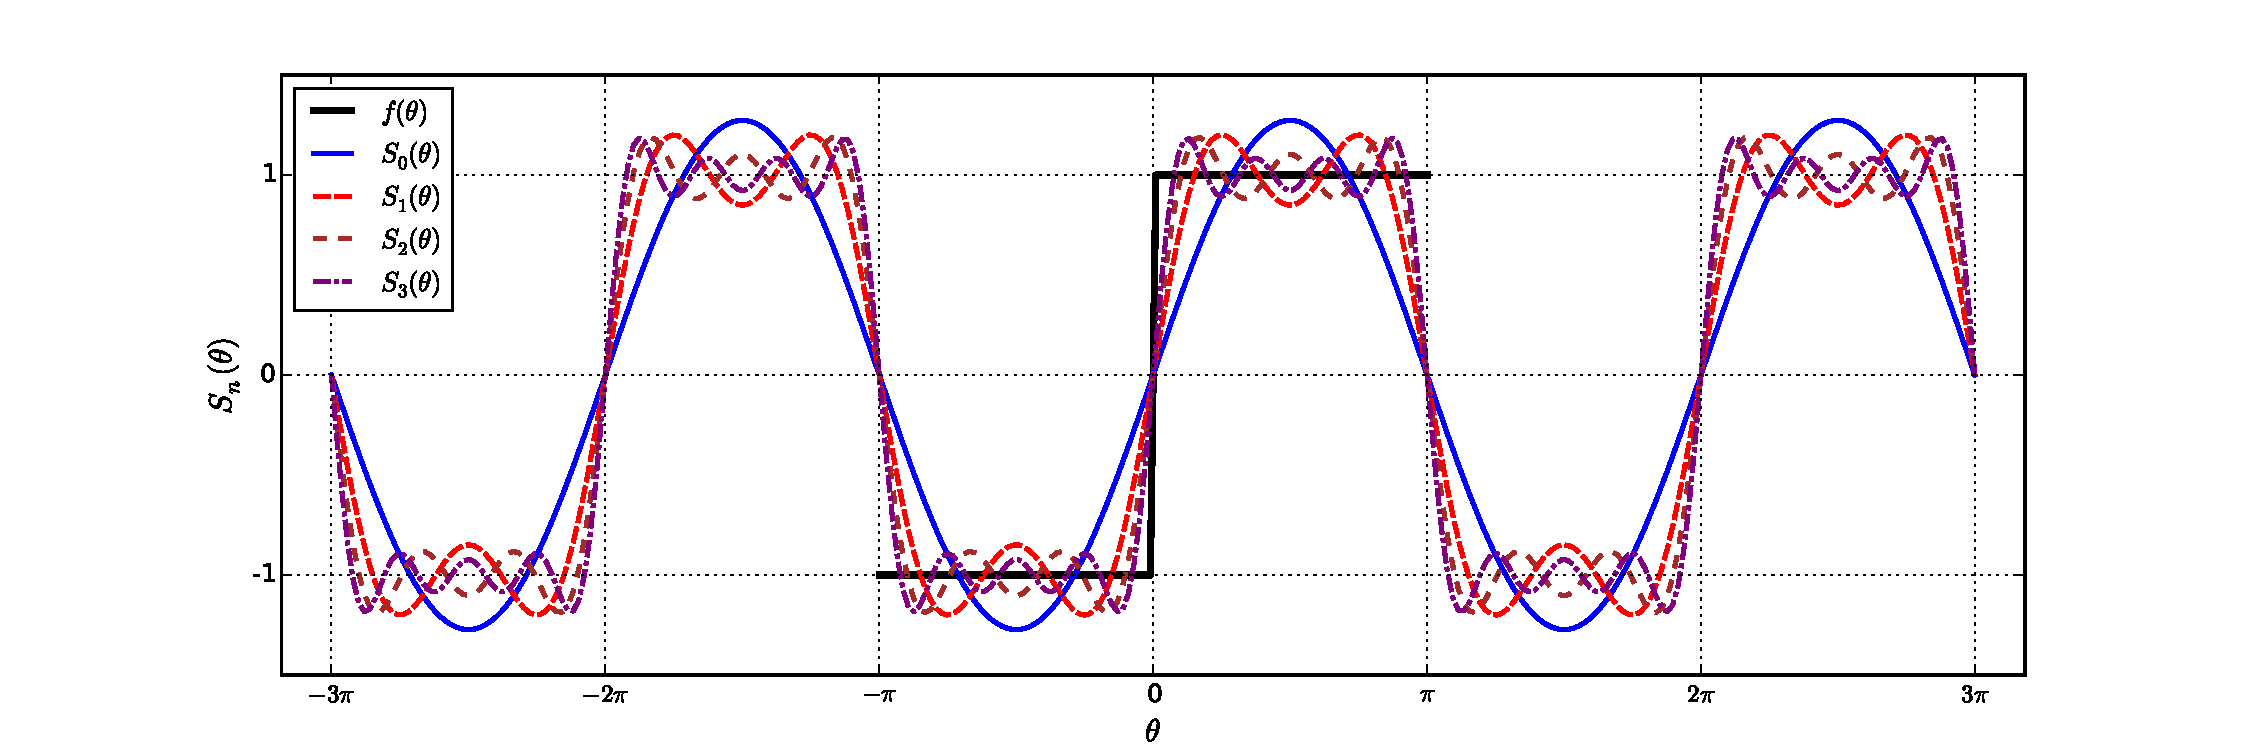
\includegraphics[scale=0.4]{figs/fig-Fourier-serie-signo.pdf}
\caption{Serie de Fourier de la funci'on Signo, truncada hasta $n=3$. Código Python disponible \href{https://github.com/gfrubi/FM2/blob/master/figuras-editables/fig-Fourier-serie-signo.py}{aquí}. Notebook interactivo \href{https://github.com/gfrubi/FM2/blob/master/Notebooks/Ejemplo-Serie-Fourier-Funcion-Signo.ipynb}{aquí}.}
\label{im:signo}
\end{figure}

\subsection{Convoluci'on}

La relaci'on o ``Teorema'' de Convoluci'on establece una relaci'on entre los coeficientes $c_{n}^{(1\cdot 2)}$ de la expansi'on de Fourier de la funci'on producto $f_1(\theta)f_2(\theta)$ y los respectivos coeficientes $c_{n}^{(1)}$ y $c_{n}^{(2)}$ de las funciones $f_1(\theta)$ y $f_2(\theta)$. El teorema establece que
\begin{equation}\label{conv}
\boxed{c_n^{(1\cdot 2)} = \sum_{m=-\infty}^{+\infty} c_m^{(2)}c_{n-m}^{(1)}.}
\end{equation}

Esto puede ser demostrado por medio del siguiente cálculo:
\begin{align}
c_n^{(1\cdot 2)} &= \frac{1}{2\pi}\int_{-\pi}^\pi f_1(\theta)f_2(\theta)e^{-in\theta}\,d\theta \\
 &= \frac{1}{2\pi}\sum_m \int_{-\pi}^\pi f_1(\theta)c_m^{(2)}e^{im\theta}e^{-in\theta}\,d\theta \\
 &= \frac{1}{2\pi}\sum_m c_m^{(2)}\int_{-\pi}^\pi f_1(\theta)e^{-i(n-m)\theta}\,d\theta \\
 &= \sum_m c_m^{(2)}c_{n-m}^{(1)}.
\end{align}


\subsection{Relaci'on de Parseval}
Si elegimos $f_1(\theta)=f^\ast (\theta)$, $f_2(\theta)=f(\theta)$ y $n=0$ en (\ref{conv}), encontramos
\begin{equation}
\boxed{\int_{-\pi}^\pi |f(\theta)|^2\,d\theta 
% &= \frac{\pi}{2} a_0^2 +\pi\sum_{n = 1}^\infty (a_n^2 + b_n^2) \\
=  2\pi\sum_{m=-\infty}^\infty\left|C_m\right|^2.}
 \end{equation}

\subsection{Convergencia}
Existen distintas nociones de convergencia de una función. Por ejemplo, es útil definir la \textbf{convergencia en media} y la \textbf{convergencia uniformemente}, de la forma siguiente:
\begin{itemize}
\item Una sucesi'on $S_n(\theta)$ de funciones definidas en el intervalo $\theta\in[-\pi,\pi]$ \textit{converge en media} a una funci'on $f(\theta)$ si
\begin{equation}
\lim_{n\to\infty}\int_{-\pi}^{\pi}\left[f(\theta)-S_n(\theta)\right]^2d\theta=0.
\end{equation}
Si esto ocurre se dice que ``La sucesi'on $S_n$ converge en media a $f(\theta)$'' lo cual significa que los valores de ambas funciones coinciden en el límite $n\to\infty$ excepto (a lo sumo) en un conjunto de medida cero.

\item Una sucesi'on $S_n(\theta)$ de funciones \textit{converge uniformemente} a una funci'on $f(\theta)$ si para todo $\epsilon>0$ existe un $N>0$ tal que
\begin{equation}
\left|f(\theta)-S_n(\theta)\right|<\epsilon, \qquad \forall n>N,
\end{equation}
para cada $\theta$ ($N$ independiente de $\theta$).
\end{itemize}

\textbf{Teorema 1} \cite{Butkov}: Si $f(\theta)$ es una funci'on ``muy suave por tramos'' (es decir, si la funci'on, su primera y segunda derivadas son continuas por tramos) en el intervalo $(-\pi,\pi)$ entonces su serie de Fourier converge a
\begin{equation}
\frac{1}{2}\left[f(\theta-0)+f(\theta+0)\right], \qquad \theta\in (-\pi,\pi),
\end{equation}
\begin{equation}
\frac{1}{2}\left[f(-\pi+0)+f(\pi-0)\right], \qquad \theta=\pm\pi .
\end{equation}
La convergencia es \textit{uniforme} en cada subintervalo cerrado donde $f(\theta)$ es \textit{continua}.

\textbf{Teorema 2} \cite{Butkov}: Si una funci'on definida en un intervalo cerrado $[a,b]$ satisface las condiciones de Dirichlet (es decir, si $f(\theta)$ es continua por tramos, y si el intervalo $(a,b)$ puede ser dividido en un n'umero finito de subinteralos donde $f(\theta)$ es monotona) entonces tambi'en se satisfacen las propiedades de convergencia del Teorema 1.

\textbf{Teorema 3} \cite{Butkov}: Si la funci'on $f(\theta)$ es \textit{cuadrado-integrable} en $(-\pi,\pi)$ ($f\in {\cal L}^2(-\pi,\pi)$, es decir, si $\int_{-\pi}^\pi|f(\theta)|^2d\theta$ es finito) entonces su serie de Fourier \textit{converge en media} a $f(\theta)$.

\textbf{Ojo!:} Esto no cubre todas las posibilidades de convergencia! Ej. $f(\theta)=\ln(\cos(\theta/2))$ (Ver \cite{Butkov}, pag.  168).

\subsection{Fen'omeno de Gibbs}

Si la funci'on $f(\theta)$, continua por tramos, posee una \textit{discontinuidad} en un punto $\theta_0$, si bien la serie truncada converge uniformemente en puntos en la vecindad de $\theta_0$, 'esta siempre sobreestima/subestima el valor de la funci'on en puntos cercanos a $\theta_0$. La regi'on donde ocurre esta sobreestimaci'on/subestimaci'on es cada vez m'as peque\~na a medidad que se agregan t'erminos a la serie truncada, \textit{pero el monto de la sobreestimaci'on/subestimaci'on es siempre finito}. De hecho, se puede mostrar\footnote{Ver por ejemplo \cite{Arfken}, cap'itulo 14.} que la serie de Fourier sobreestima el ``salto'' de la funci'on en la discontinuidad por aproximadamente $17.9\%$.

\section{Cambio de Intervalo}
Es simple extender los resultados anteriores al caso de funciones peri'odicas de periodo arbitrario. Si $f(t)$ es una funci'on de periodo $T=b-a$ entonces
\begin{equation}\label{defgt}
g(\theta):=f(a+\frac{T}{2\pi}\theta)
\end{equation}
es una funci'on de periodo $2\pi$ en la variable $\theta$. Por lo tanto, podemos expandir $g(\theta)$ en serie de Fourier,
\begin{equation}\label{sfgt}
g(\theta)=\sum_{n=-\infty}^\infty c_n e^{i n\theta}, \qquad c_n =\frac{1}{2\pi}\int_{-\pi}^\pi g(\theta) e^{-in\theta}\,d\theta .
\end{equation}
Usando (\ref{defgt}), y realizando el cambio de variable de integraci'on a $t:=a+T\theta/2\pi$,  podemos expresar los coeficientes $c_n$ como
\begin{align}
c_n =& \frac{1}{2\pi}\int_{-\pi}^\pi g(\theta) e^{-in\theta}\,d\theta  \\
=& \frac{1}{2\pi}\int_{-\pi}^\pi f(a+\frac{T}{2\pi}\theta) e^{-in\theta}\,d\theta \\
=& \frac{1}{2\pi}\int_{a-T/2}^{b-T/2} f(t) e^{-in\frac{2\pi}{T}(t-a)}\frac{2\pi}{T}dt \\
=& \frac{1}{T}e^{\frac{2\pi ina}{T}}\int_a^b f(t) e^{-\frac{2\pi i n}{T}t}\,dt.
\end{align}
Definimos la \textbf{frecuencia fundamenal} $\omega_1:=2\pi/T$ y las \textbf{frecuencias arm'onicas} $\omega_n:=n\omega_1$, $n=0,\pm 1, \pm 2, \cdots$. Entonces, la funci'on original $f(t)=g(2\pi(t-a)/T)$ puede escribirse como
\begin{equation}\label{ftpT}
\boxed{f(t)=\sum_n f_n\, e^{i\omega_n t},}
\end{equation}
donde
\begin{equation}\label{fnpT}
\boxed{f_n:=\frac{1}{T}\int_a^b f(t) e^{-i\omega_n t}\,dt.}
\end{equation}

\subsection{Delta de Dirac}
Podemos encontrar una representaci'on de la (extensi'on peri'odica de la) delta de Dirac $\delta(t)$ (ver ap'endice \ref{app:Dirac} para m'as detalles) en t'erminos de una serie de Fourier. En este caso, los coeficientes $f_n$ se reducen a:
\begin{align}
f_n &= \frac{1}{T}\int_a^b \delta(t) e^{-i\omega_n t}\,dt \\
&= \frac{1}{T}.
\end{align}

Por lo tanto,
\begin{equation}
\delta(t)=\frac{1}{T}\sum_n \, e^{i\omega_n t}=\frac{1}{T}\left[1+2\sum_{n=1}^\infty\cos\left(\frac{2\pi n t}{T}\right)\right].
\end{equation}

Definimos el $k$-'esimo t'ermino de la serie como 
\begin{align}
T_{k}(t):=\left\{
\begin{array}{cl}
\frac{1}{T}, &\text{si } k=0\\
\frac{2}{T}\sum_{k=1}^{\infty}\cos\left(\frac{2\pi k t}{T}\right), &\text{si } k=1,2,\ldots
\end{array} \right. ,
\end{align}
y la serie de Fourier truncada hasta el t'ermino $n$-'esimo en la forma:
\begin{align}
S_n(t):=\sum_{k=0}^n T_{k}(t).
\end{align}

Es importante notar, como puede comprobarse al graficar la serie, que lo que se obtiene es en realidad la \textit{extensi'on peri'odica} (de periodo $T$) de la delta de Dirac.
\begin{figure}[H]
\centering
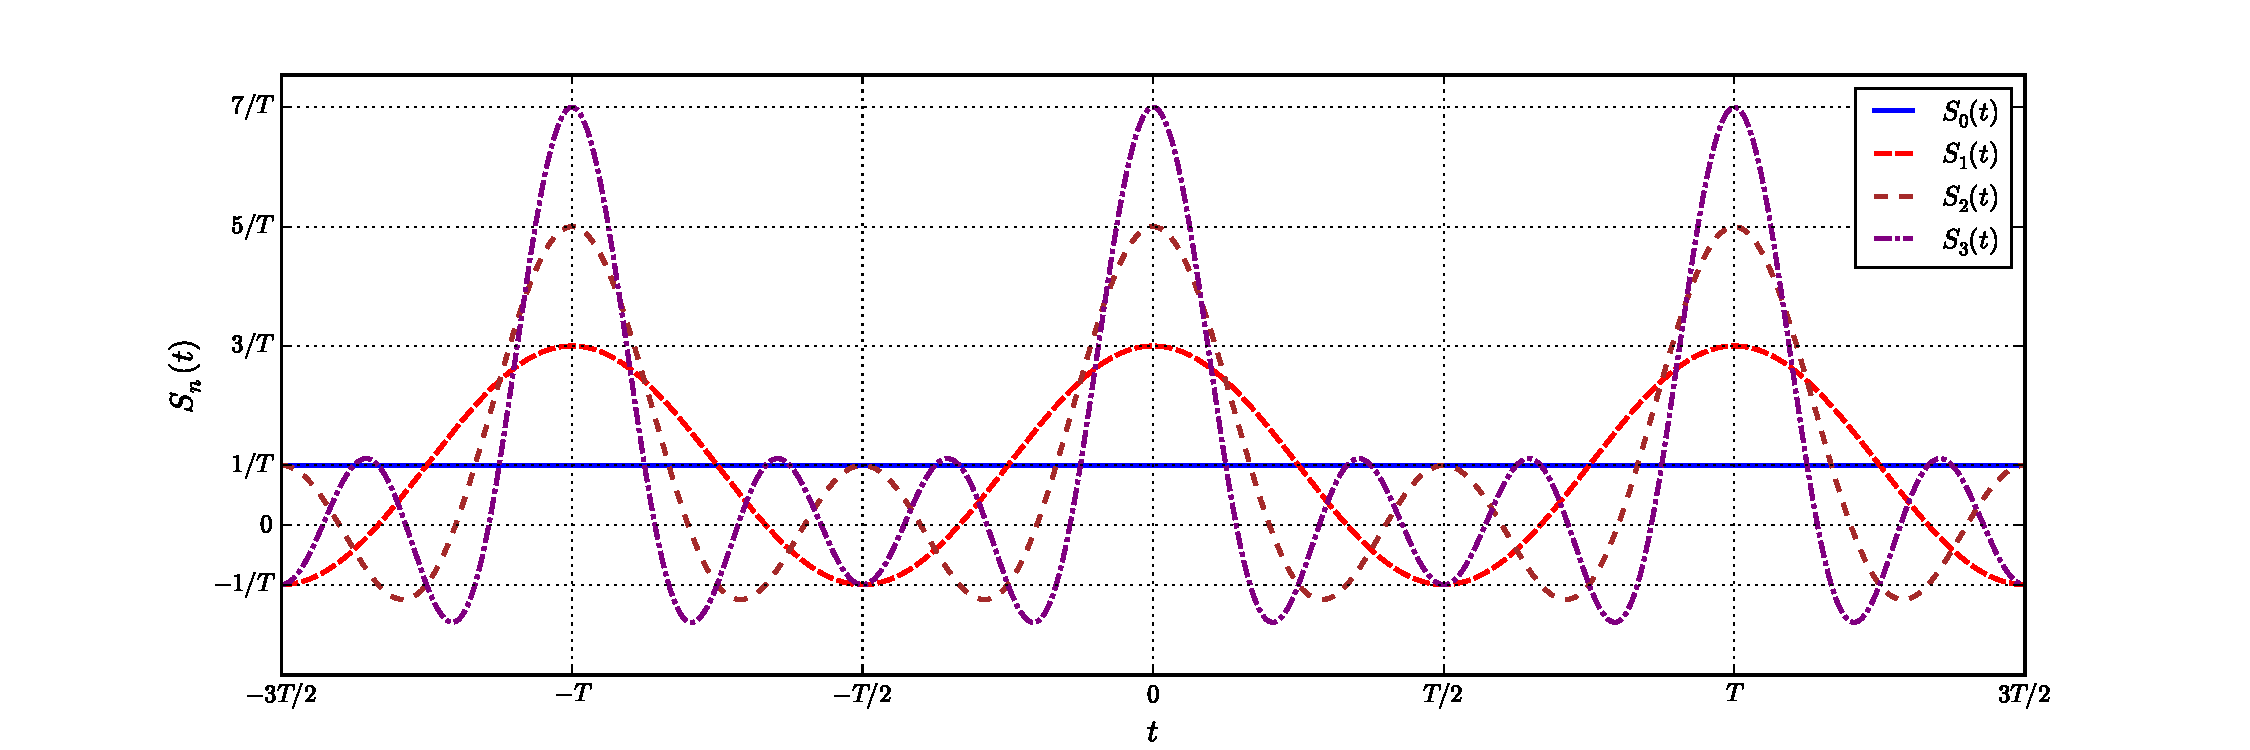
\includegraphics[scale=0.4]{figs/fig-Fourier-serie-Dirac}
\caption{Serie de Fourier de la delta de Dirac con per'iodo $T=2\pi$, truncada hasta $n=4$. Código Python disponible \href{https://github.com/gfrubi/FM2/blob/master/figuras-editables/fig-Fourier-serie-Dirac.py}{aquí}.}
\label{im:delta}
\end{figure}


\chapter{La transformada de Fourier}

Las series de Fourier permiten representar una funci'on \textit{peri'odica} como superposici'on de funciones seno y coseno (o exponenciales de argumento imaginario). Es posible extender el m'etodo de expansi'on de Fourier al caso de funciones no-peri'odicas, resultando las llamadas \textbf{integrales de Fourier}. Podemos entender estas integrales de Fourier como el \textit{l'imite cont'inuo} de las series de Fourier.

Consideremos una funci'on $f(t)$ de periodo $T$, y como intervalo fundamental a $(-T/2,T/2)$. Entonces, usando (\ref{ftpT}) y (\ref{fnpT}) podemos escribir
\begin{equation}\label{fcont1}
f(t) =\sum_{n = -\infty}^\infty\left[\frac{1}{T}\int_{-T/2}^{T/2} f(\xi) e^{-i\omega_n\xi}\, d\xi\right] e^{i\omega_nt}.
\end{equation}
Equivalentemente, podemos expresar la suma en (\ref{fcont1}) en t'erminos de la frecuencias $\omega_n$ y la diferencia (en este caso, constante) entre ellas $\Delta\omega:=\omega_{n+1}-\omega_n=2\pi/T$:
\begin{equation}
f(t) =\sum_{\omega_n = -\infty}^\infty\left[\frac{1}{2\pi}
\int_{-T/2}^{T/2} f(\xi) e^{-i\omega_n\xi}\,d\xi\right] e^{i\omega_n t}\Delta\omega.
\end{equation}
En el l'imite $T\to\infty$, (y por lo tanto $\Delta\omega\to 0$), la funci'on $f(t)$ puede considerarse como una funci'on no-peri'odica arbitraria definida en todo el intervalo $(-\infty,\infty)$. Por otro lado, la suma se transforma en una integral\footnote{Recuerde la definici'on de integral de Riemann: $\int_a^bf(x)\,dx:=\lim_{\Delta x_i\to 0}\sum_{x_i}f(x_i)\Delta x_i$.}. Por lo tanto, en este l'imite obtenemos la identidad
\begin{equation}\label{idfnp}
f(t) =\int_{-\infty}^\infty\left[\frac{1}{2\pi}\int_{-\infty}^\infty
 f(\xi) e^{-i\omega\xi}\,d\xi\right] e^{i\omega t}\,d\omega,
\end{equation}
a partir de la cual podemos definir la \textbf{transformada de Fourier} de la funci'on $f(t)$ como
\begin{equation}\label{TFf}
\boxed{\tilde{f}(\omega) :=\int_{-\infty}^\infty f(t) e^{-i\omega t}\,dt,}
\end{equation}
de modo que la ``transformada inversa'' resulta ser
\begin{equation}\label{TFIf}
\boxed{f(t)=\frac{1}{2\pi}\int_{-\infty}^\infty\tilde{f}(\omega) e^{i\omega t} \,d\omega.}
\end{equation}



Observaciones:

\begin{itemize}
\item Cuidado! La derivaci'on anterior es ``heur'istica'' (e.d. no rigurosa). 
\item Otras notaciones: $\tilde{f}(\omega)=g(\omega)={\cal F}(f)(\omega)$.
\item El factor $1/2\pi$ en la definici'on (\ref{TFIf}) es hasta cierto punto convencional (usado, por ejemplo, por el módulo \texttt{Sympy} de Python). Lo importante es la identidad (\ref{idfnp}). Por ejemplo, en lugar de estos factores, podr'ia introducirse $\alpha$ en (\ref{TFf}) y $1/2\pi\alpha$ en (\ref{TFIf}), con una constante $\alpha$ arbitraria. Otras elecciones populares son $\alpha=1$ y $\alpha=1/\sqrt{2\pi}$ (Arfken \cite{Arfken}; Hassani \cite{Hassani}; Riley, Hobson \& Bence \cite{Riley}).
\item Note que en (\ref{TFIf}) la integral se extiende sobre ``frecuencias positivas y negativas''.
\item Compare (\ref{TFf}) con la definici'on de la \textbf{transformada de Laplace}: $F(s):=\int_0^\infty f(t)e^{-st}dt$.
\item En F'isica es costumbre denotar, en el caso en que se considere una funci'on de la posici'on, $f(t)\to f(x)$ y usar el \textit{n'umero de onda} $k$ en lugar de la frecuecia $\omega$, de modo que la expansi'on adopta la forma $f(x)=(1/{2\pi})\int_{-\infty}^\infty\tilde{f}(k) e^{ikx} \,dk.$
\end{itemize}

\subsection{Ejemplo: Pulso cuadrado}
Como primer ejemplo, consideramos la función $f(x)$ definida por
\begin{equation}
f(x)=\begin{cases}
1, & |x|<a \\
0, & |x|>a
\end{cases}.
\end{equation}
En este caso, la transformada resulta ser
\begin{equation}
\tilde{f}(k)=\frac{2\sin(ka)}{k}.
\end{equation}
\begin{figure}[h]
\centering
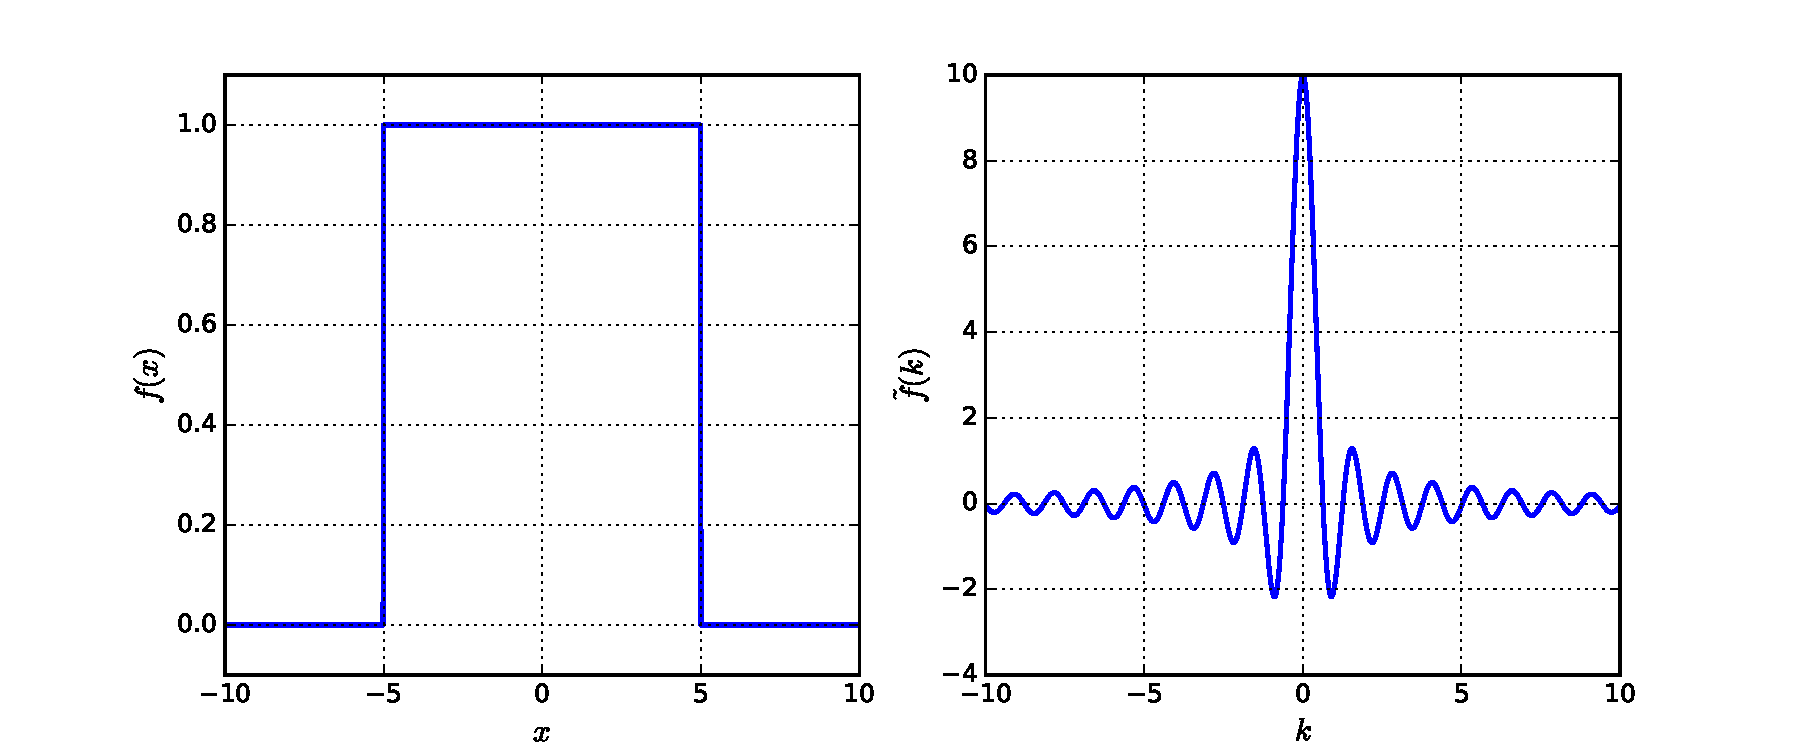
\includegraphics[scale=0.4]{figs/fig-transformada-Fourier-pulso-cuadrado.pdf}
\caption{Pulso cuadrado y su transformada de Fourier, con $a=5$.}
\label{im:pulsocua}
\end{figure}

\subsection{Ejemplo: Distribuci'on Gaussiana}
Considere la \textbf{distribuci'on gaussiana} definida por
\begin{equation}\label{fgauss}
f(t):= e^{-\alpha t^2}, \qquad \alpha>0,
\end{equation}
entonces su transformada de Fourier es dada por
\begin{align}
\tilde{f}(\omega) &= \int_{-\infty}^{\infty}e^{-\alpha t^2} e^{-i \omega t}dt\notag \\
&= \int_{-\infty}^{\infty}e^{-\alpha t^2-i\omega t} dt.
\end{align}
Notando que
\begin{align}
-\alpha t^2-i\omega t=&-\alpha \left(t^2+\frac{i\omega}{\alpha}t\right) \notag \\
=&-\alpha\left(t^2+\frac{i\omega}{\alpha}t+\left(\frac{i\omega}{2\alpha}\right)^2-\left(\frac{i\omega}{2\alpha}\right)^2\right) \notag \\
=&-\alpha \left( t+\frac{i\omega}{2\alpha} \right)^2+\alpha\left(\frac{i\omega}{2\alpha}\right)^2\notag \\
=&-\alpha \left( t+\frac{i\omega}{2\alpha} \right)^2-\left(\frac{\omega^2}{4\alpha}\right),
\end{align}
se halla entonces que
\begin{align}
\tilde{f}(\omega)=&\int_{-\infty}^{\infty}e^{-\alpha \left( t+\frac{i\omega}{2\alpha} \right)^2-\left(\frac{\omega^2}{4\alpha}\right)}dt\notag\\
=& e^{-\frac{\omega^2}{4\alpha}}\int_{-\infty}^{\infty}e^{-\alpha \left( t+\frac{i\omega}{2\alpha} \right)^2}dt,
\end{align}
pero haciendo el cambio de variables $x:=\sqrt{\alpha}(t+i\omega/4\alpha)$, entonces $dx=\sqrt{\alpha}\,dt$, luego
\begin{align}
\tilde{f}(\omega)=e^{-\frac{\omega^2}{4\alpha}}\int_{-\infty}^{\infty}e^{-x^2} \frac{dx}{\sqrt{\alpha}}.
\end{align}
Adem'as, recordando que
\begin{align}
\int_{-\infty}^{\infty}e^{-x^2}dx=\sqrt{\pi},
\end{align}
encontramos finalmente que
\begin{equation}\label{Tfgauss}
{\cal F}[e^{-\alpha t^2}]=\sqrt{\frac{\pi}{\alpha}}e^{-\frac{\omega^2}{4\alpha}}.
\end{equation}
\begin{figure}[h]
\centering
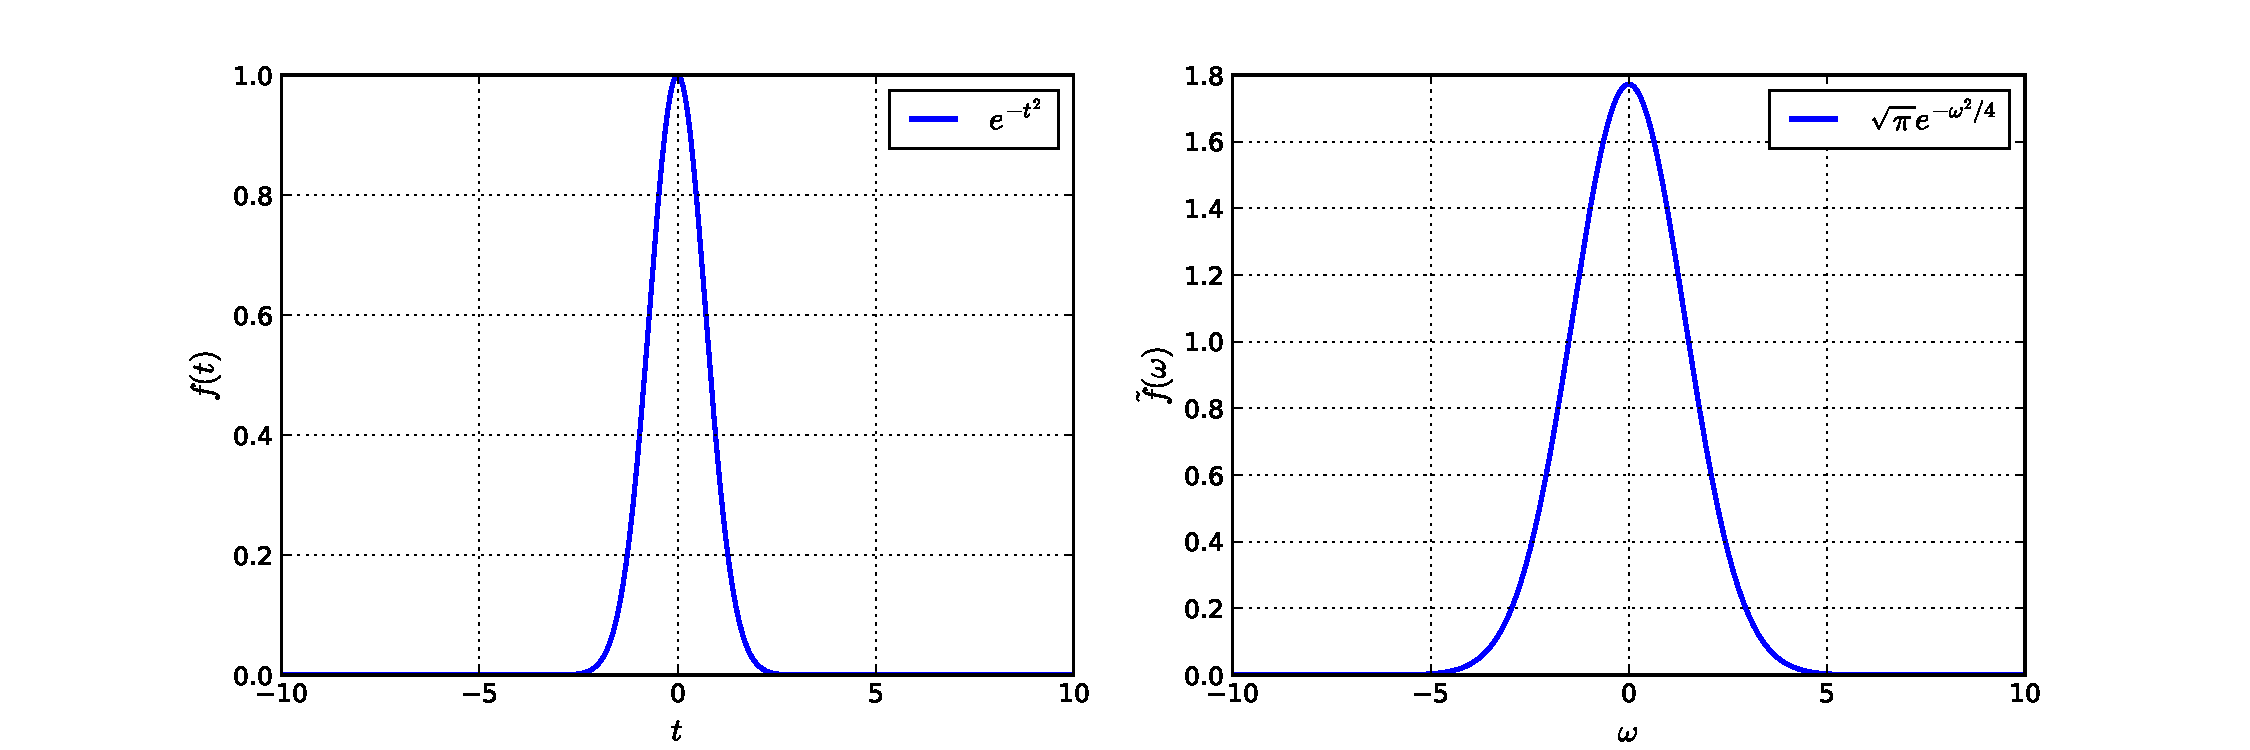
\includegraphics[scale=0.4]{figs/fig-Fourier-Gaussiana.pdf}
\caption{Distribuci'on gaussiana y su transformada de Fourier con $\alpha=1$.}
\label{im:gaussiana}
\end{figure}

\textbf{Tarea:} Verifique que, efectivamente, la transformada inversa reproduce la funci'on original, es decir,
\begin{equation}\label{Tfinvgauss}
{\cal F}^{-1}[e^{-\frac{\omega^2}{4\alpha}}]=\sqrt{\frac{\alpha}{\pi}}e^{-\alpha t^2}.
\end{equation}

\section{Propiedades de la Transformada de Fourier} 
\subsection{Linealidad}
\begin{equation}
{\cal F}[\alpha f_1(t)+\beta f_2(t)](\omega) = \alpha{\cal F}[f_1(t)](\omega)+\beta {\cal F}[f_2(t)](\omega).
\end{equation}
\subsection{Complejo conjugado}
\begin{equation}
{\cal F}[f^\ast(t)](\omega) = \left({\cal F}[f(t)](-\omega)\right)^\ast.
\end{equation}

\subsection{Delta de Dirac}
\begin{align}
{\cal F}[\delta(t-\xi)] 
 &=\int_{-\infty}^\infty\delta(t-\xi) e^{-i\omega t}\,dt 
\\
 &=e^{-i\omega\xi} \label{Fd}
\end{align}
\begin{equation}
\boxed{ 
\delta(t-\xi) =\frac{1}{2\pi}\int_{-\infty}^\infty e^{i\omega (t-\xi)}\,d\omega. 
 }
\end{equation}
%
\subsection{Transformada de Fourier de la derivada de una funci'on}
\begin{align}
{\cal F}[f'(t)]
 &=\int_{-\infty}^\infty f'(t) e^{-i\omega t}\,dt \\
 &=\left[ f(t) e^{-i\omega x}\right]_{-\infty}^\infty
 -\int_{-\infty}^\infty (-i\omega) f(t) e^{-i\omega t}\,dt \\
 &=\left[ f(t) e^{-i\omega x}\right]_{-\infty}^\infty+ i\omega\int_{-\infty}^\infty f(t) e^{-i\omega t}\,dt \\
 &= i\omega{\cal F}[f(t)]+\left. f(t) e^{-i\omega t}\right|_{-\infty}^\infty.\label{eq:trans-fourier-derivada-gen}
\end{align}
Entonces, \textit{si la funci'on $f(t)$ se anula en el infinito}, es decir si $\lim_{t\to\pm\infty}f(t)=0$, tendremos que
\begin{equation}
\boxed{ 
{\cal F}\left[f'(t)\right] = (i\omega){\cal F}[f(t)]. \label{eq:trans-fourier-derivada-esp}
 } 
\end{equation} 
Aplicaci'on sucesiva de esta relaci'on, bajo las mismas condiciones, conduce a
\begin{equation}
\boxed{ 
{\cal F}\left[f^{(n)}(t)\right] = (i\omega)^n{\cal F}[f(t)]. 
 } 
\end{equation} 



\subsubsection{Ejemplo: Funci'on escal'on.}
Sea la funci'on escal'on $H(t)$ tal que
\begin{equation}
H_c(t) := 
\begin{cases}
0, &\text{si }t < c,\\
1, &\text{si }t > c
\end{cases},
\end{equation}

\begin{figure}[h]
\centering
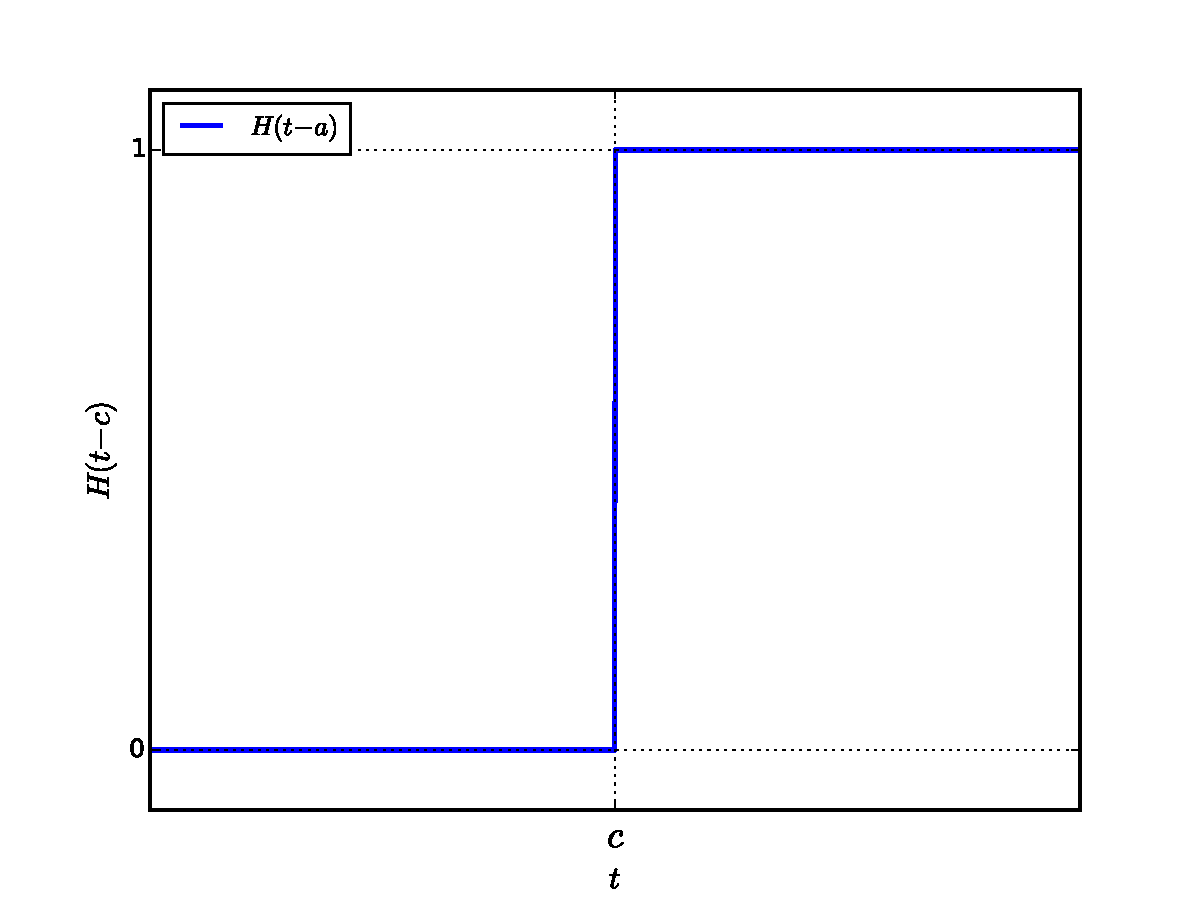
\includegraphics[scale=0.4]{figs/fig-funcion-escalon.pdf}
\caption{Funci'on escal'on.}
\label{im:escalon}
\end{figure}
con la interesante propiedad que
\begin{equation}
\frac{dH}{dt}(t) = \delta(t-c).
\end{equation}
Es de relevancia mencionar que ingenuamente podr'iamos pasar por alto el hecho que la funci'on escal'on no satisface la hip'otesis que $\lim_{t\to\pm\infty}H(t-c)=0$ y recordando \eqref{Fd} podr'iamos pretender calcular la transformada de Fourier simplemente usando la expresi'on \eqref{eq:trans-fourier-derivada-esp}, lo que nos conducir'ia err'oneamente a que
\begin{equation}
\boxed{ {\cal F}[H(t-c)] =\frac{1}{i\omega} e^{-i c\omega}.}
\end{equation}
Sin embargo, al emplear directamente la definici'on de la transformada de Fourier vemos que
\begin{align}
{\cal F}[H](\omega)=&\int_{-\infty}^{\infty}H(t)e^{-i\omega t}dt\notag \\
=&\int_{c}^{\infty}1\cdot e^{-i\omega t}dt\notag \\
=&\left.\frac{e^{-i\omega t}}{-i\omega}\right|_{c}^{\infty}, \label{TFH}
\end{align}
y debido a que
\begin{align}
\left.\frac{e^{-i\omega t}}{-i\omega}\right|_{\infty}=\lim_{t \rightarrow \infty}\frac{e^{-i\omega t}}{-i\omega}
\end{align}
no existe (el l'imite no tiende a un valor 'unico), entonces se concluye que la transformada de Fourier de la funci'on escal'on tampoco. Sin embargo, la relaci'on  completa \eqref{eq:trans-fourier-derivada-gen} sigue siendo v'alida y suministra una expresi'on equivalente a \eqref{TFH}.
%
\subsection{Teorema de Convoluci'on}
El teorema de convoluci'on suministra una 'util relaci'on entre la transformada de Fourier de un producto de funciones y las transformadas de Fourier de cada una de las funcioes.
\begin{align}
{\cal F}[f_1(t)f_2(t)]
 &=\int_{-\infty}^\infty f_1(t)f_2(t) e^{-i\omega t}\,dt \\
 &=\frac{1}{2\pi}\int_{-\infty}^\infty f_1(t) \left(\int_{-\infty}^\infty\tilde{f}_2(\omega')
 e^{i\omega' t}\,d\omega'\right)e^{-i\omega t}\,dt \\
 &=\frac{1}{2\pi}\int_{-\infty}^\infty\left(\int_{-\infty}^\infty f_1(t) 
 e^{-i(\omega-\omega')t}\,dt\right)\tilde{f}_2(\omega')\,d\omega' \\
 &=\frac{1}{2\pi} \int_{-\infty}^\infty\tilde{f}_1(\omega-\omega')\tilde{f}_2(\omega')\,d\omega'.
\end{align}
Por lo tanto, 
\begin{equation}\label{TeocovTF}
\boxed{{\cal F}[f_1(t)f_2(t)] = \tilde{f}_{1\cdot 2}(\omega)=\frac{1}{2\pi} \int_{-\infty}^\infty\tilde{f}_1(\omega-\omega')\tilde{f}_2(\omega')\,d\omega' .
 } 
\end{equation}   
An'alogamente, la relaci'on entre las transformadas inversas es
\begin{equation}
{\cal F}^{-1}[\tilde{f}_1(\omega)\tilde{f}_2(\omega)]
=\int_{-\infty}^\infty f_1(\xi)f_2(t-\xi)\,d\xi .	
\end{equation}



\subsubsection{Ejemplo} Usando el teorema de convoluci'on podemos encontrar la transformada de Fourier de 
\begin{equation}\label{ejTFconv}
 f(t) =\frac{1}{t^4 + 5 t^2 + 4} = \frac{1}{(t^2+1)(t^2+4)}.
\end{equation}
ya que
\begin{equation}
{\cal F}\left[\frac{c}{t^2+c^2}\right] = \pi e^{-c |\omega|},\qquad\text{ para }c > 0. 
\end{equation}
\begin{align}
{\cal F}[f(t)]
 &={\cal F}\left[\frac{1}{t^2+1}\frac{1}{t^2+4}\right] 
\\
 &=\frac{1}{2\pi}\frac{\pi}{1}\frac{\pi}{2}\left(\int_{-\infty}^\infty e^{-|\eta|} e^{-2|\omega -\eta|}\,d\eta\right) 
\\
 &=\frac{\pi}{4}\left(\int_{-\infty}^0 e^\eta e^{-2|\omega -\eta|}\,d\eta
 +\int_0^\infty e^{-\eta} e^{-2|\omega -\eta|}\,d\eta\right)
\end{align}
Si $\omega > 0$,
\begin{align}
{\cal F}[f(t)]
 &=\frac{\pi}{4}\left(\int_{-\infty}^0 e^{-2\omega + 3\eta}\,d\eta
 +\int_0^\omega e^{-2\omega +\eta}\,d\eta
 +\int_\omega^\infty e^{2\omega - 3\eta}\,d\eta\right) 
\\
 &=\frac{\pi}{4}\left(\frac{1}{3} e^{-2\omega} + e^{-\omega}
 - e^{-2\omega} +\frac{1}{3} e^{-\omega}\right) 
\\
 &=\frac{\pi}{2}\left[ \frac{2}{3}e^{-\omega} -\frac{1}{3} e^{-2\omega}\right].
\end{align}
Si $\omega < 0$,
\begin{align}
{\cal F}[f(t)]
 &=\frac{\pi}{4}\left(\int_{-\infty}^\omega e^{-2\omega+3\eta}\,d\eta
 +\int_\omega^0 e^{2\omega -\eta}\,d\eta
 +\int_0^\infty e^{2\omega-3\eta}\,d\eta\right) 
\\
 &=\frac{\pi}{4}\left(\frac{1}{3} e^\omega - e^{2\omega}
 + e^\omega +\frac{1}{3} e^{2\omega}\right)\\
 &=\frac{\pi}{2}\left[\frac{2}{3}e^\omega -\frac{1}{3} e^{2\omega} \right].
\end{align}
Podemos expresar los resultados para ambos signos de $\omega$ como:
\begin{equation}
\boxed{ 
{\cal F}[f(t)] =\frac{\pi}{2}\left[\frac{2}{3} e^{-|\omega|} -\frac{1}{3} e^{-2|\omega|} \right].
 } 
\end{equation} 
Otra forma de encontrar la transformada de \eqref{ejTFconv} es expandir la funci'on en fracciones parciales:
\begin{equation}
f(t) =\frac{1}{3}\frac{1}{t^2 + 1} -\frac{1}{3}\frac{1}{t^2 + 4},
\end{equation}
\begin{align}
{\cal F}[f(t)]
&=\frac{1}{3}{\cal F}\left[\frac{1}{t^2 + 1}\right]
-\frac{1}{3}{\cal F}\left[\frac{1}{t^2+4}\right]\\
&=\frac{1}{3}\frac{\pi}{1} e^{-|\omega|} -\frac{1}{3}\frac{\pi}{2} e^{-2|\omega|}.
\end{align}        

\subsection{Teorema de Parseval}
\begin{equation}
\boxed{
\int_{-\infty}^\infty |f(t)|^2\,dt=\frac{1}{2\pi}\int_{-\infty}^\infty |\tilde{f}(\omega)|^2\,d\omega.
 }
\end{equation}
En forma análoga al caso de la relación de Parseval para una serie de Fourier, el resultado anterior puede ser encontrado como caso particular del Teorema de Convolución \eqref{TeocovTF}, eligiendo $f_1(t)=f(t)$, $f_2(t)=f^\ast(t)$ y $\omega=0$.
\subsection{Ancho de la funci'on y su transformada}

Definimos el \textbf{valor medio} de $t$ respecto a la funci'on (distribuci'on) $f(t)$ como
\begin{equation}
\langle t \rangle:=\frac{\int f^{*}(t) t f(t)\,dt}{\int |f(t)|^{2}\, dt}=\frac{\int t |f(t)|^2\,dt}{\int |f(t)|^2\,dt}
\end{equation}
y, an'alogamente, el valor medio de $\omega$ respecto a la transformada $\tilde{f}(\omega)$ por
\begin{equation}
\langle \omega \rangle:=\frac{\int \tilde{f}^{*}(\omega) \omega \tilde{f}(\omega) d\omega}{\int |\tilde{f}(\omega)|^{2} d\omega}=\frac{\int \omega |\tilde{f}(\omega)|^2 d\omega}{\int |\tilde{f}(\omega)|^2 d\omega}.
\end{equation}
De forma similar, la \textbf{varianza} de $t$ respecto a $f(t)$ es definida por
\begin{equation}
(\Delta t)^2:=\frac{\int f^{*}(t)(t-\langle t \rangle)^2 f(t)\,dt}{\int |f(t)|^2\, dt}=\frac{\int (t- \langle t \rangle)^2 |f(t)|^2 t}{\int |f(t)|^2 dt}.
\end{equation}
Finalmente, la varianza de $\omega$ respecto a $\tilde{f}(\omega)$ es dada por:
\begin{equation}
(\Delta \omega)^2:=\frac{\int \tilde{f}^{*}(\omega)(\omega-\langle \omega \rangle)^2 \tilde{f}( \omega) d\omega}{\int |\tilde{f}(\omega)|^2 d\omega}=\frac{\int (\omega- \langle \omega \rangle)^2 |\tilde{f}(\omega)|^2 \omega}{\int |\tilde{f}(\omega)|^2 d\omega}.
\end{equation}


Sea $f(t)$ una funci'on tal que $\lim_{t \rightarrow \pm \infty} f(t)=0$ y $f'=df/dt$, entonces $\tilde{f'}=i \omega \tilde{f}$, y podemos escribir $\omega \tilde{f}=-i \tilde{f'}$. Por lo tanto
\begin{align}
(\Delta \omega)^2 \int |\tilde{f}|^2 d\omega =&\int |i\tilde{f'}+\langle \omega \rangle \tilde{f}|^2 d \omega \notag \\
=&\int |{\cal F}[if'+\langle \omega \rangle f]|^2 d\omega.
\end{align}
Pero empleando el teorema de Parseval se encuentra que
\begin{align}
(\Delta \omega)^2 \int |\tilde{f}|^2 d\omega &= 2\pi\int |if'+\langle \omega \rangle f]|^2 dt.
\end{align}
Recordando la desigualdad (triangular) de Schwarz, que establece que $\forall f_{1},f_{2}$ se cumple que
\begin{align}
\left( \int |f_{1}|^2 dt \right)\left( \int |f_{2}|^2 dt\right) \geq \left|\int f_{1}^{*}f_{2}dt\right|,
\end{align}
y considerando $f_{1}(t):=(t-\langle t \rangle)f(t)$ y $f_{2}(t):=if'(t)+\langle \omega \rangle f(t)$, se tiene que
\begin{align}
\left(\int |f|^2 dt \right) (\Delta t)^2 \cdot (\Delta \omega)^2 \left(\int |f|^2 dt \right)\geq
\left|\int f^{*}(t)(t-\langle t \rangle)\left(if'(t)+ \langle\omega\rangle f(t)\right) dt\right|^2.
\end{align}
Si definimos $I$ como la integral del segundo miembro de la ecuaci'on precedente, podemos hallar que
\begin{align}
I=&\int \left[ i f^{*}t f'+\langle \omega \rangle f^{*} t f-\langle t \rangle i f^{*}f'-\langle t \rangle \langle \omega \rangle |f|^2\right]dt  \notag \\
=&i\int \left(f^{*} t \frac{df}{dt}-\langle t \rangle f^{*} \frac{df}{dt} \right) dt+\langle \omega \rangle \langle t \rangle \int |f|^2 dt-\langle t \rangle \langle \omega \rangle \int |f|^2 dt\notag \\
=&i \int f^{*}(t-\langle t\rangle)\frac{df}{dt} dt.
\end{align}
Notando que
\begin{align}
{\rm Im}(I) &= \frac{1}{2}\int \left[ f^{*}(t-\langle t \rangle)\frac{df}{dt}+\left(\frac{df}{dt}\right)^{*}(t-\langle t \rangle)f\right]dt\notag \\
&= \frac{1}{2}\int \left( \frac{d}{dt}[f^{*}(t-\langle t \rangle)f]-f^{*}f\right)dt\notag \\
&= \left. \frac{1}{2} (t-\langle t \rangle)|f|^2 \right|_{-\infty}^{\infty}-\frac{1}{2}\int |f|^2 dt.
\end{align}
Para que $\int |f|^2 dt$ y $\langle t \rangle$ sean finitos, suponemos que $|f|^2\rightarrow 0$ y $t|f^2| \rightarrow 0$ cuando $t \rightarrow \pm \infty$. En tal caso
\begin{align}
{\rm Im}(I)=-\frac{1}{2}\int |f|^2 dt.
\end{align}
Adem'as, como $|I|^2=[{\rm Re}(I)]^2+[{\rm Im}(I)]^2\geq [{\rm Im}(I)]^2$, podemos escribir que
\begin{align}
(\Delta t)^2 (\Delta \omega)^2 \left(\int |f|^2 dt \right)^2 \geq [{\rm Im}(I)]^2= \frac{1}{4} \left( \int |f|^2 dt\right)^2,
\end{align}
de donde se deduce que
\begin{align}
(\Delta t)^2 \cdot (\Delta\omega)^2 \geq \frac{1}{4}
\end{align}
o, finalmente,
\begin{align}\label{DtDo}
\boxed{
\Delta t\cdot \Delta\omega\ge\frac{1}{2}.
}
\end{align}

\subsubsection{Ejemplo}
Un ejemplo instructivo es el caso de la funci'on gaussiana \eqref{fgauss}. En este caso un c'alculo simple muestra que
\begin{equation}
\langle t\rangle=0,  \qquad \Delta t =\frac{1}{2\sqrt{\alpha}}.
\end{equation}
Similarmente, para la transformada \eqref{Tfgauss}, que tiene la misma forma funcional, tendremos que
\begin{equation}
\langle\omega\rangle=0,  \qquad \Delta\omega =\sqrt{\alpha}.
\end{equation}
Verificamos que en ambos casos los valores medios son una medida del ``valor central'' y que la varianza cuantifica el ``ancho'' de cada distribuci'on. La distribuci'on gaussiana es especial en el sentido que \textit{satura la desigualdad} \eqref{DtDo}, ya que en este caso
\begin{equation}
\Delta t\cdot \Delta\omega =\frac{1}{2}.
\end{equation}
\section{Generalizaci'on a mayores dimensiones}
En $D$ dimensiones:
\begin{equation}
{\cal F}[f(\vec{x})]=\tilde{f}(\vec{k})
:= \int f(\vec{x})e^{i(\vec{k}\cdot\vec{x})}d^Dx,
\end{equation}
\begin{equation}
f(\vec{x}) = {\cal F}^{-1}(\tilde{f})
:= \frac{1}{(2\pi)^{D}}\int \tilde{f}(\vec{k})e^{-i(\vec{k}\cdot\vec{x})}d^Dk.
\end{equation}

*** cambio convenci'on! listo hasta aqu'i ***


\section{Transformada de Fourier seno y coseno}











\chapter{Ecuaciones Diferenciales parciales de la F'isica}

En F'isica es com'un encontrar sistemas descritos por \textit{campos}\footnote{Es decir, funciones que dependen de la posici'on y/o del tiempo.} ($\Psi$), que satisfacen ecuaciones diferenciales parciales (EDP's). Entre las m'as
frecuentes destacan las siguientes:
\begin{itemize}
\item Ecuaci'on de Laplace: 
\begin{equation}
\nabla^2\Psi=0, \qquad \Psi(\vec{x}).
\end{equation}
 Esta ecuaci'on aparece, por ejemplo, en el estudio de:
	\begin{itemize}
	\item Electrost'atica. El \textbf{potencial el'ectrico} $\phi$ en una \textit{regi'on sin cargas} satisface la ec. de Laplace.
	\item Hidrodin'amica. Un \textit{fluido irrotacional incompresible} en un \textit{movimiento estacionario} con campo de velocidad $\vec{v}=-\vec\nabla\Psi$ satisface
	\begin{equation}
	\frac{\partial\rho}{\partial t}+\vec\nabla (\rho\vec{v})=0 \quad\Rightarrow\quad
	\vec\nabla\cdot\vec{v}=-\nabla^2\Psi=0.
	\end{equation}
	\item Distribuci'on de Temperatura estacionaria: Aqu'i $\Psi=T(\vec{x},t)$ es el campo de temperaturas de un material, la ecuaci'on del Calor, ver \eqref{eccalor},  se reduce a la ec. de Laplace para $T(\vec{x})$.
	\item Gravitaci'on. An'alogo al caso electrost'atico, con $\Psi=\phi=\text{potencial gravitacional}$.
	\end{itemize}
\item Ecuaci'on de Poisson
\begin{equation}
\nabla^2\Psi=g(\vec{x}),
\end{equation}
donde $g(\vec{x})$ es una funci'on ``fuente'' conocida. Esta EDP es \textit{inhomog'enea}, y por lo tanto sus soluciones generales pueden escribirse como $\Psi=\Psi_{\rm h}+\Psi_{\rm p}$, donde $\Psi_{\rm h}$ es soluci'on de la ecuaci'on homogenea correspondiente (en este caso, la ec. de Laplace), y $\Psi_{\rm p}$ una \textbf{soluci'on particular} de la ec. de Poisson.

Por ejemplo, el potencial electrost'atico $\phi(\vec{x})$ satisface
\begin{equation}
\nabla^2\phi=-\frac{1}{\varepsilon_0}\rho(\vec{x}),
\end{equation}
donde $\varepsilon_0$ es la \textbf{permeabilidad del vac'io} y $\rho(\vec{x})$ la \textbf{densidad (volum'etrica) de carga el'ectrica}.
\item Ecuaci'on de Helmholtz: 
\begin{equation}
\nabla^2\Psi\pm k^2\Psi=0.
\end{equation}
Esta ecuaci'on, conocida tambi'en como la ecuaci'on de difusi'on independiente de tiempo, aparece en el estudio de
	\begin{itemize}
	\item Ondas el'asticas en s'olidos.
	\item Ac'ustica.
	\item Ondas electromagn'eticas.
	\item Reactores nucleares.
	\end{itemize}
\item Ecuaci'on de difusi'on dependiente del tiempo ($\alpha= $ difusividad t'ermica)
\begin{equation}\label{eccalor}
\nabla^2\Psi-\frac{1}{\alpha}\frac{\partial \Psi}{\partial t}=0 .
\end{equation}
\item Ecuaci'on de la onda dependiente del tiempo
\begin{equation}
\nabla^2\Psi-\frac{1}{v^2}\frac{\partial^2\Psi}{\partial t^2} =0,
\end{equation}
o bien 
\begin{equation}
\square\Psi=0, \qquad \square:=\frac{1}{v^2}\frac{\partial^2\ }{\partial t^2}-\nabla^2.
\end{equation}
Esta EDP aparece en modelos de:
\begin{itemize}
\item Ondas el'asticas en s'olidos, membranas, cuerdas, etc.
\item Ondas electromagn'eticas en regiones sin fuentes.
\item Ondas sonoras.
\end{itemize}

\item Ecuaci'on de Klein-Gordon:
\begin{equation}
\square\Psi-\frac{m^2c^2}{\hbar^2}\Psi=0.
\end{equation}

\item Ecuaci'on de Schr\"odinger:
\begin{equation}
-\frac{\hbar^2}{2m}\nabla^2\Psi+V(\vec{x})\Psi=i\hbar\frac{\partial\Psi}{\partial t}.
\end{equation}
\end{itemize}

Observaciones:

\begin{itemize}
\item Todas estas ecuaciones son \textit{lineales} en la funci'on desconocida.
\item Las ecuaciones fundamentales de la f'isica atmosf'erica son no-lineales, as'i como tambi'en las ecuaciones involucradas en los problemas de turbulencia.
\item Estas ecuaciones son casi todas de segundo orden excepto las ecuaciones de Maxwell y de Dirac que son de primer orden.
\end{itemize}

Las t'ecnicas generales para (intentar) resolver \textit{EDP lineales} que consideraremos en este curso son:
\begin{enumerate}
\item \textbf{M'etodo de separaci'on de variables}: La ecuaci'on diferencial parcial es desdoblada en ecuaciones diferenciales ordinarias lineales. La soluci'on de la EDP es construida como superposici'on de soluciones que son el producto de funciones dependientes de cada variable. Usando este m'etodo es posible reducir la ec. de la onda, la ec. del calor, y la ec. de Klein-Gordon a la ec. de Helmholtz.
\item \textbf{M'etodo de las transformadas integrales} (Fourier, Laplace, etc.), para resolver EDP inhomog'eneas.
\item \textbf{M'etodo de las funciones de Green}, para resolver EDP inhomog'eneas.

\end{enumerate}

\section{Clasificaci'on de E.D.P. lineales de segundo orden y Condiciones de Borde}

Una E.D.P. \textit{lineal de segundo orden} de la forma \cite{Hassani}
\begin{equation}\label{EDP2O}
\sum_{j=1}^m a_j(\vec{x})\frac{\partial^2\Psi}{\partial x_j^2}+F\left(\vec{x},\Psi,\vec\nabla\Psi\right)=0,
\end{equation}
o que pueda reducirse a (\ref{EDP2O}) por medio de alg'un cambio de variables, puede clasificarse en los siguientes tres tipos:
\begin{itemize}
\item \textbf{El'ipticas en $\vec{x}_0$:} si en el punto $\vec{x}_0$ todos los coeficientes $a_j(\vec{x}_0)$ son no-nulos y tienen \textit{el mismo signo}. Ejemplo cl'asico: Ec. de Laplace.
\item \textbf{Ultrahiperb'olicas en $\vec{x}_0$:} si en el punto $\vec{x}_0$ todos los coeficientes $a_j(\vec{x}_0)$ son no-nulos, pero \textit{no tienen el mismo signo}. Si s'olo uno de los coeficientes tiene signo diferente del resto, la E.D.P. es \textbf{hiperb'olica}. Ejemplo cl'asico: Ec. de onda.
\item \textbf{Parab'olica en $\vec{x}_0$:} si en el punto $\vec{x}_0$ al menos uno de los coeficientes $a_j(\vec{x}_0)$ se anula. Ejemplo cl'asico: Ec. de difusi'on del calor.
\end{itemize}
Si una E.D.P. de segundo orden es de un tipo dado en todos los puntos de su dominio, se dice simplemente que es de ese tipo (es decir, el tipo no cambia de punto a punto). Esto ocurre, en particular con las E.D.P.'s de segundo orden con coeficientes constantes.

\subsection{Condiciones de Borde y condiciones suficientes para determinar soluciones}
La soluci'on de une EDP requiere especificar informaci'on adicional a la ecuaci'on. Esta informaci'on recibe el nombre de \textbf{Condiciones de Borde} (C. de B.), o \textbf{condiciones de Frontera}, o bien \textbf{condiciones iniciales} y generalizan las conficiones iniciales necesarias para resulver una EDO.

En el caso de EDP's de segundo orden, existen tres tipos principales de C. de B.:

\begin{itemize}
\item C. de B. \textbf{tipo Dirichlet}: donde el valor de la funci'on ($\Psi$) es especificada en la frontera de la regi'on considerada.
\item C. de B. \textbf{tipo Neumann}: donde el valor de la \textbf{derivada normal de funci'on en la frontera} ($\partial\Psi/\partial t:=\hat{n}\cdot\vec\nabla\Psi$) es especificada.
\item C. de B. \textbf{tipo Cauchy}: donde se especifican \textit{simultaneamente} C. de B. tipo Dirichlet y Neumann en la frontera.
\end{itemize}
Por ejemplo, en electroest'atica (donde el potencial electrost'atico $\phi$ satisface la ecuaci'on de Poisson), una C. de B. tipo Dirichlet significa especificar un valor del potencial en la frontera, mientras que una C. de B. tipo Neumann equivale a especificar el valor de la componente del campo el'ectrico normal a la frontera. 

Existen teoremas de existencia y unicidad de soluciones de EDP's de segundo orden, dependiendo de si la ecuaci'on es parab'olica, hiperb'olica o el'iptica:

\textbf{Teorema:} Existe soluci'on 'unica en cada uno de los siguientes casos:

\begin{itemize}
\item E.D.P. el'ipticas +  C.de B. tipo \textit{Dirichlet o Neumann} sobre una (hiper)superficie \textit{cerrada}.
\item E.D.P. hiperb'olica + C.de B. tipo \textit{Cauchy} sobre una (hiper)superficie \textit{abierta}.
\item E.D.P. parab'olica + C.de B. tipo \textit{Dirichlet o Neumann} sobre una (hiper)superficie \textit{abierta}.
\end{itemize}

\subsection{Ejemplo: Difusi'on del calor $1-$dimensional}

Resolver la ecuaci'on de difusi´on del calor $1-$dimensional, empleando la transformada de Fourier espacial y temporal e imponiendo la siguiente condiciones de contorno
\begin{align}
\lim_{x \rightarrow \pm \infty}\psi(x,t)=0,\label{eq:bc1}\\
\psi(x,0)=\phi(x).\label{eq:bc2}
\end{align}

Como el problema es $1-$dimensional, la ecuaci'on a resolver es
\begin{align}
\alpha \frac{\partial^2 \psi}{\partial^2 x}-\frac{\partial \psi}{\partial t}=0,
\end{align}
as'i, aplicando la tranformada de Fourier espacial a la ecuaci'on precendente, se tiene que
\begin{align}
\alpha {\cal F}_{x}[\frac{\partial^2 \psi}{\partial^2 x}]-{\cal F}_{x}[\frac{\partial \psi}{\partial t}]=0,
\end{align}
adem'as por la condici'on de contorno \eqref{eq:bc1} se tiene que
\begin{align}
\frac{\partial^2 \psi}{\partial^2 x}=(i k)^2 \tilde{\psi}(k,t),
\end{align}
y como
\begin{align}
{\cal F}_{x}[\frac{\partial \psi}{\partial t}]=\frac{\partial}{\partial t}{\cal F}_{x}[\psi],
\end{align}
entonces
\begin{align}
-\alpha k^2 \tilde{\psi}(k,t)-\frac{\partial}{\partial t}\tilde{\psi}(k,t)=0,
\end{align}
por lo tanto
\begin{align}
\frac{\partial}{\partial t}\tilde{\psi}(k,t)=-\alpha \tilde{\psi}(k,t),
\end{align}
e integrando parcialmente en la variable $t$ se halla que
\begin{align}
\tilde{\psi}(k,t)=\tilde{\psi}(k,0)e^{-\alpha k^2 t}.
\end{align}
Por otro lado, empleando la condición \eqref{eq:bc2} vemos que
\begin{align}
{\cal F}_{x}[\psi(x,0)]={\cal F}_{x}[\psi(x)]\notag \\
\tilde{\psi}(k,0)=\tilde{\phi}(k),
\end{align}
en consecuencia
\begin{align}
\tilde{\psi}(k,t)=\tilde{\phi}(k)e^{-\alpha k^2 t}.
\end{align}
En efecto, la soluci'on del problema es
\begin{align}
\psi(x,t)=&\frac{1}{\sqrt{2\pi}}\int_{-\infty}^{\infty}\tilde{\psi}(k,t)e^{ikx} dk\notag \\
=&\frac{1}{\sqrt{2\pi}}\int_{-\infty}^{\infty}\tilde{\phi}(k)e^{-\alpha k^2 t}e^{ikx} dk,
\end{align}
con
\begin{align}
\tilde{\phi}(k)=\frac{1}{\sqrt{2\pi}}\int_{-\infty}^{\infty}\phi(x)e^{ikx}dx.
\end{align}
En particular, si suponemos
\begin{align}
\phi(x)=T_{0}\delta(x),
\end{align}
entonces
\begin{align}
\tilde{\phi}(k)=T_{0}{\cal F}_{x}[\delta(x)]=\frac{T_{0}}{\sqrt{2\pi}}.
\end{align}
Por consiguiente
\begin{align}
\psi(x,t)=\frac{T_{0}}{2\pi}\int_{-\infty}^{\infty}e^{-\alpha k^2 t} e^{ikx}dk
=\frac{T_{0}}{2\pi}\int_{-\infty}^{\infty}e^{-\alpha k^2 t+ikx}dk,
\end{align}
pero completando cuadrados vemos que
\begin{align}
-\alpha k^2 t+ikx=&-\alpha t \left( k^2-\frac{ikx}{\alpha t}\right)\notag \\
=&-\alpha t \left( k^2-\frac{ikx}{\alpha t}+\left(\frac{ix}{2\alpha t}\right)^2-\left(\frac{ix}{2\alpha t}\right)^2\right)\notag \\
=&-\alpha t\left( \left(k-\frac{ix}{2\alpha t} \right)^2 +\frac{x^2}{4 \alpha^2 t^2}\right)\notag \\
=& -\alpha t \left(k-\frac{ix}{2\alpha t} \right)^2-\frac{x^2}{4 \alpha t},
\end{align}
luego
\begin{align}
\psi(x,t)=&\frac{T_{0}}{2\pi}\int _{-\infty}^{\infty}e^{-\frac{x^2}{4 \alpha t}} e^{-\alpha t \left(k-\frac{ix}{2\alpha t} \right)^2} dk\notag \\
=&\frac{T_{0} e^{-\frac{x^2}{4 \alpha t}}}{2\pi}\int _{-\infty}^{\infty}e^{-\alpha t \left(k-\frac{ix}{2\alpha t} \right)^2} dk,
\end{align}
y haciendo el cambio de variables $y:=\sqrt{\alpha t}(k-ix/2\alpha t)$ se tiene que $dy=\sqrt{\alpha t} dk$, entonces
\begin{align}
\psi(x,t)=&\frac{T_{0} e^{-\frac{x^2}{4 \alpha t}}}{2\pi}\int _{-\infty}^{\infty}e^{-y^2} \frac{dy}{\sqrt{\alpha t}},
\end{align}
Por lo tanto, se ha hallado que\footnote{En \url{http://nbviewer.ipython.org/urls/dl.dropbox.com/s/0dgalwtzh6cr33m/difusion-calor.ipynb?dl=0} puede visualizar un notebook con la animaci'on de la soluci'on.}
\begin{align}
\psi(x,t)=&\frac{T_{0}}{2\sqrt{\pi \alpha t}}e^{-\frac{x^2}{4 \alpha t}}\qquad \forall t>0.
\end{align}

\chapter{El M'etodo de Separaci'on de Variables}

El m'etodo de separaci'on de variables (MSV, originalmente introducido por Daniel Bernoulli, 1700-1782) para encontrar soluciones de EDP's \textit{lineales} consiste en reducir la EDP a un conjunto de EDO's para un conjunto de funciones auxiliares. Cada una de estas funciones auxiliares depende s'olo de una de las variables independientes del problema. La soluci'on es entonces construida como una \textit{superposici'on} (e.d. combinaci'on lineal) de \textbf{soluciones separables}, consistentes en productos de las funciones auxiliares.

M'as expl'citamente, el MSV consiste en:
\begin{itemize}
\item Buscar soluciones separables de la EDP. Esto conduce a un conjunto de EDO's.
\item Construir una superposici'on general de soluciones separables, e imponer las condiciones de contorno y/o iniciales del problema.
\end{itemize}

Si bien en general el MSV sigue los pasos anteriores, en la pr'actica es 'util considerar un paso intermedio:
\begin{itemize}
\item Imponer las condiciones de contorno/iniciales homog'eneas a cada funci'on separable. Esto simplifica mucho el c'alculo puesto que t'ipicamente elimina muchas posibles contribuciones a la (futura) combinaci'on lineal. Esto s'olo puede ser realizado con las condiciones de borde/iniciales homog'eneas para EDP's lineales y homog'eneas, puesto que si la soluci'on separable satisface estas condiciones entonces cualquier superposici'on lineal lo har'a. Adem'as, no se pierde generalidad con este m'etodo, puesto que (puede demostrarse que) las funciones separables obtenidas son linealmente independientes.
\end{itemize}

En resumen, es conveniente aplicar el MSV de la siguiente forma:
\begin{itemize}
\item Buscar soluciones separables de la EDP (conjunto de EDO's).
\item Imponer las condiciones de borde/iniciales \textit{homog'eneas} a las soluciones separables.
\item Construir una combinaci'on lineal general con las soluciones separables anteriores.
\item Determinar los coeficientes de la combinaci'on lineal que aseguran que la soluci'on final satisface las \textit{condiciones de borde/iniciales inhomog'eneas}.
\end{itemize}



\section{Coordenadas Cartesianas}
\section{Ejemplo: Ecuaci'on de Laplace en dominio rectangular}
Buscaremos la soluci'on $\Psi(x,y)$ que satisface la ecuaci'on de Laplace bidimensional
\begin{equation}\label{ejLap2D}
\frac{\partial^2\Psi }{\partial x^2}+\frac{\partial^2\Psi }{\partial y^2}=0,
\end{equation}
en el rect'angulo $0<x<1$, $0<y<2$, con la condici'on de borde
\begin{equation}
\Psi(x,2) = x(1-x), 
\end{equation}
y con $\Psi=0$ en los otros tres lados. 

Primero buscamos soluciones separables de la EDP, de la forma
\begin{equation}
\Psi_{\rm sep}(x,y)=X(x)Y(y).
\end{equation}
Al reemplazar en \eqref{ejLap2D} y dividir por $\Psi_{\rm sep}$ encontramos
\begin{equation}
\frac{1}{X(x)}\frac{d^2X}{dx^2}+\frac{1}{Y(y)}\frac{d^2Y}{dy^2} = 0,
\end{equation}
lo que implica que t'ermino debe ser igual a una constante, es decir
\begin{equation}
\frac{1}{X(x)}\frac{d^2X}{dx^2} = \lambda, \qquad \frac{d^2X}{dx^2}-\lambda X(x)=0,
\end{equation}
\begin{equation}
\frac{1}{Y(y)}\frac{d^2Y}{dy^2} = -\lambda, \qquad \frac{d^2Y}{dy^2}+\lambda Y(y)=0.
\end{equation}
La forma expl'icita de estas ecuaciones depende del valor, y en particular del signo, de la constante de separaci'on $\lambda$, que por ahora tiene valor desconocido: Por ejemplo,
\begin{equation}
X_\lambda(x)= 	\begin{cases}
		c_1e^{\sqrt{\lambda}x} + c_2e^{-\sqrt{\lambda}x}, & \text{si }\lambda>0 \\
		c_1 + c_2x,  & \text{si } \lambda=0 \\
		c_1\cos(\sqrt{-\lambda}x) + c_2\sin(\sqrt{-\lambda}x), & \text{si } \lambda<0
		\end{cases}.
\end{equation}
Similarmente,
\begin{equation}
Y_\lambda(y)= 	\begin{cases}
		\bar{c}_1\cos(\sqrt{\lambda}y) + \bar{c}_2\sin(\sqrt{\lambda}y), & \text{si }\lambda>0 \\
		\bar{c}_1 + \bar{c}_2y,  & \text{si } \lambda=0 \\
		\bar{c}_1e^{\sqrt{-\lambda}y} + \bar{c}_2e^{-\sqrt{-\lambda}y}, & \text{si } \lambda<0
		\end{cases}.
\end{equation}
As'i, hemos encontrado infinitas soluciones separables, cada una de la forma
\begin{equation}\label{EjLapPsiXY}
\Psi_\lambda^{\rm sep}(x,y)=X_\lambda(x)Y_\lambda(y),
\end{equation}
para cada valor posible de la constante de separaci'on $\lambda$. Como esta constante puede tomar distintos valores, y como la EDP es \textit{lineal}, entonces cualquier combinaci'on lineal de la forma
\begin{equation}\label{EjLapPsisumaSep}
\Psi(x,y) = \sum_{\lambda}\Psi_\lambda^{\rm sep}(x,y) = \sum_{\lambda}X_\lambda(x)Y_\lambda(y),
\end{equation}
es tambi'en soluci'on.

Procedemos ahora a imponer las condiciones de borde a la soluci'on. Los c'alculos se simplifican si imponemos primero las \textit{condiciones de borde homog'eneas}. Por ejemplo, la condici'on $\Psi(0,y)=0$, $\forall y\in[0,2]$ (borde izquierdo del dominio) requiere que
\begin{equation}
\Psi(0,y) = \sum_{\lambda}\Psi_\lambda^{\rm sep}(0,y) = \sum_{\lambda}X_\lambda(0)Y_\lambda(y) = 0.
\end{equation}
La 'ultima expresi'on es una combinaci'on lineal de los coeficientes (constantes) $X_\lambda(0)$ y las funciones $Y_\lambda(y)$. Ya que las funciones $Y_\lambda(y)$ son l.i. en esta combinaci'on ser'a nula s'olo si $X_\lambda(0)=0$. An'alogamente, la condici'on 
$\Psi(1,y)=0$, $\forall y\in[0,2]$ requiere $X_\lambda(1)=0$. Estas dos condiciones sobre las funciones $X_\lambda(x)$ restringen fuertemente los valores posibles de $\lambda$. En nuestro caso particular, s'olo valores negativos de esta constante de separaci'on son permitidos. Esto ocurre si $\lambda = -n^2\pi^2$, $n=1,2,\dots$, y entonces
\begin{equation}
X_n(x)=c_n\sen\left(n\pi x\right), \qquad \lambda = -n^2\pi^2, \qquad n=1,2,\dots.
\end{equation}

Para estos valores de $\lambda$, las soluciones para $Y(y)$ son de la forma
\begin{equation}
Y_n(y) = \bar{c}_1e^{\pi ny} + \bar{c}_2e^{-\pi ny}.
\end{equation}

Imponemos ahora la condici'on de borde en la frontera inferior del dominio, es decir, $\Psi(x,0) = 0$, lo que se traduce en $Y_n(0)=0$. Esto s'olo puede ser satisfecho si $\bar{c}_1+\bar{c}_2=0$, por lo que la soluci'on se reduce a
\begin{equation}
Y_n(y) = \bar{c}_1\left(e^{\pi ny} -e^{-\pi ny}\right) = 2\bar{c}_1 \senh(\pi ny).
\end{equation}

Con esto, la soluci'on adopta la forma
\begin{equation}\label{ejLap2D2}
\Psi(x,y) = \sum_{n=0}^\infty d_n \sen\left(n\pi x\right)\senh(\pi ny),
\end{equation}
donde los coeficientes son arbitrarios. Es instructivo verificar que esta expresi'on es soluci'on de la EDP \eqref{ejLap2D}, y de las condiciones de borde homog'eneas del problema. El valor de los coeficientes $d_n$ queda determinado por la condici'on de borde no-homog'enea restante (borde superior).

Imponemos por tanto que
\begin{equation}
\Psi(x,2) = \sum_{n=0}^\infty d_n \sen\left(n\pi x\right)\senh(2\pi n) \stackrel{!}{=} f(x),
\end{equation}
con $f(x)=x(1-x)$. Esto significa que los coeficientes $d_n\senh(2\pi n)$ son los coeficientes de la expansi'on de Fourier (seno) de la funci'on $f(x)$ en el intervalo $[0,1]$. Usando las relaciones de ortogonalidad de las funciones $\senh(\pi nx)$, 
\begin{equation}
\int_0^1 \senh(\pi nx)\senh(\pi mx)\,dx = \frac{1}{2}\delta_{nm},
\end{equation}
encontramos
\begin{equation}
d_n\senh(2\pi n) = 2 \int_0^1 f(x)\senh(\pi nx)\,dx,
\end{equation}
y por lo tanto
\begin{equation}
d_n = \frac{2}{\senh(2\pi n)} \int_0^1 f(x)\senh(\pi nx)\,dx.
\end{equation}

En el ejemplo particular en que $f(x)=x(1-x)$, luego de calcular la integral correspondiente, encontramos que
\begin{equation}
d_n = \begin{cases}
	\frac{8}{\pi^3n^3}\senh(2\pi n) , & \text{para } n \text{ impar} \\
	0 , & \text{para } n \text{ par} \end{cases}
\end{equation}

Con todo esto, y denotanto $n=2k-1$, con $k=1,2,3,\cdots$, encontramos que nuestra soluci'on es dada por la siguiente serie:
\begin{equation}
\psi(x,y)=\frac{8}{\pi^3}\sum_{k=1}^{\infty}\frac{\sin[(2k-1) \pi x]}{(2k-1)^3}\frac{\sinh[(2k-1)\pi y]}{\sinh[2\pi (2k-1)]}.
\end{equation}

\begin{figure}[H]
\centering
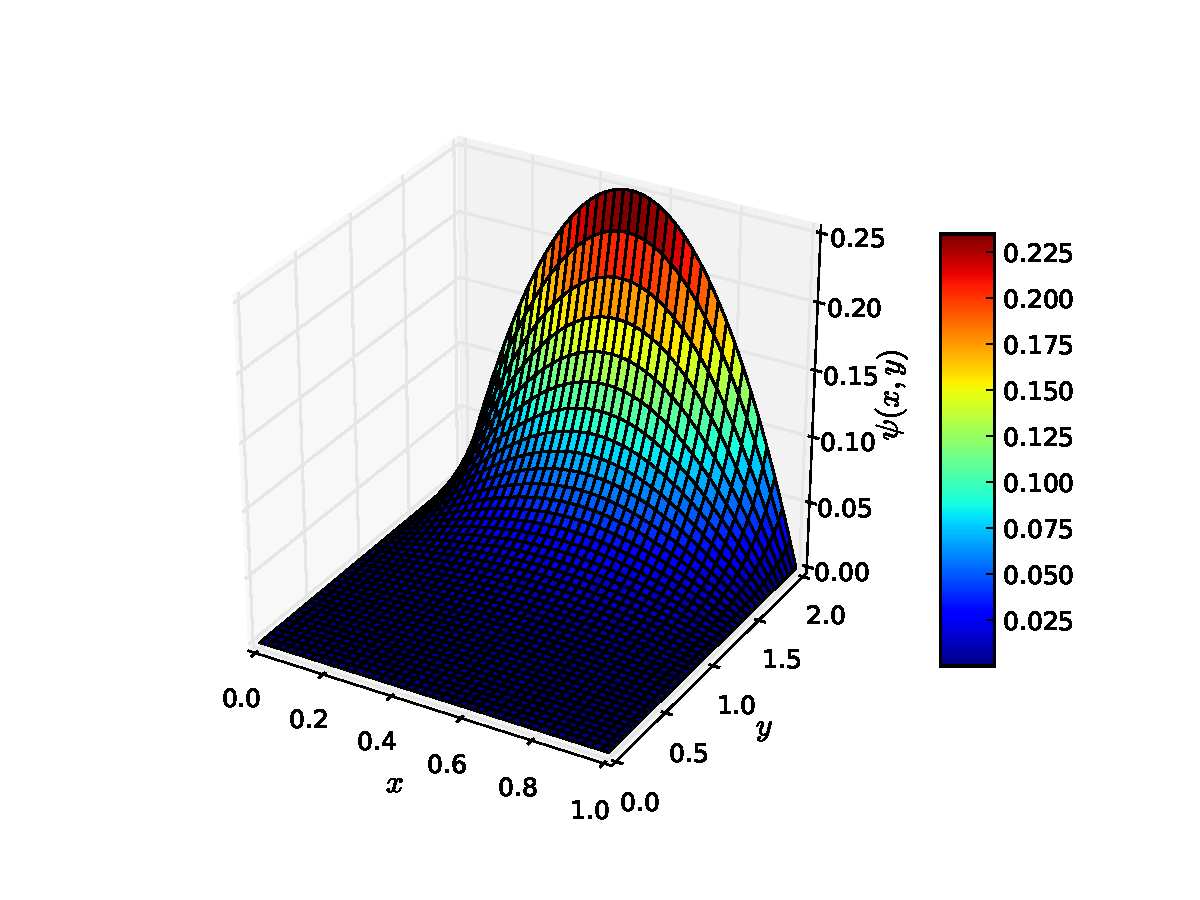
\includegraphics[angle=0,width=0.7\textwidth]{figs/fig-MSV-rectangulo-3D.pdf}
\caption{La soluci'on a nuestro problema, en 3D.}
\label{fig-SolLap}
\end{figure}

\subsection{Ejemplo: Ecuaci'on de onda en $1-$dimensi'on.}
Resolver la ecuaci'on de onda $1-$dimensional empleando el m'etodo de separaci'on de variables e imponiendo las siguientes condiciones de contorno 
\begin{align}
\psi(0,t)=0,\qquad \psi(L,t)=0,\label{eq:cond-borde}
\end{align}
y las siguientes condiciones iniciales 
\begin{align}
\psi(x,0)=\psi_{0}(x),\qquad \frac{\partial \psi}{dt}(x,0)=v_{0}(x),\label{eq:cond-inicial}
\end{align}
suponiendo que $\psi_{0}(x)$ y $v_{0}(x)$ son dadas pero arbitrarias de la variable $x$.

Como el problema a resolver es $1-$dimensional, la ecuaci'on a resolver es
\begin{align}
\frac{\partial^2 \psi}{\partial x^2}-\frac{1}{v^2}\frac{\partial^2 \psi}{\partial t^2}=0.\label{eq:ec-onda}
\end{align}

As'i, al emplear el MSV y suponer una soluci'on del tipo $\psi(x,t)=X(x)T(t)$, entonces
\begin{align}
\frac{\partial^2 \psi}{\partial x^2}=T(t) \frac{d^2X}{dx^2}(x),\qquad \frac{\partial^2 \psi}{\partial t^2}=X(x) \frac{d^2 T}{dt^2}(x),
\end{align}
de esta forma, al introducir las ecuaciones precedentes en \eqref{eq:ec-onda} se halla que
\begin{align}
T(t) \frac{d^2X}{dx^2}(x)-\frac{1}{v^2}X(x) \frac{d^2 T}{dt^2}(t)=0,
\end{align}
pero al dividir la ecuaci'on anterior por $\psi$, suponiendo que $\psi \neq 0$, entonces
\begin{align}
\frac{1}{X}\frac{d^2 X}{dx^2}=\frac{1}{v^2}\frac{1}{T}\frac{d^2 T}{dt^2}.\label{eq:ec-separable}
\end{align} 

Como el primer miembro de la ecuaci'on \eqref{eq:ec-separable} depende de $x$ y el segundo miembro de $t$, es evidente que ambos deben ser constantes con respecto a ambas variables, vale decir
\begin{align}
\frac{1}{X}\frac{d^2 X}{dx^2}=\lambda \text{  y  }\frac{1}{v^2}\frac{1}{T}\frac{d^2 T}{dt^2}=\lambda,
\end{align}
donde $\lambda$ es llamada la ``constante de separaci'on''. Luego podemos escribir la siguiente EDO para $X=X(x)$
\begin{align}
\frac{d^2 X}{dx^2}=\lambda X,
\end{align}
cuya soluci'on est'a condicionada por los posibles valores que tome la constante de separaci'on. Es directo verificar que
\begin{align}
X(x)=
\begin{cases}
A \cos(x\sqrt{-\lambda})+B \sin(x\sqrt{-\lambda}), & \text{si }\lambda<0\\
A' x+B', & \text{si }\lambda=0\\
A'' e^{x\sqrt{\lambda}}+B'' e^{-x\sqrt{\lambda}}, & \text{si }\lambda >0
\end{cases}.
\end{align}

Ahora bien, al imponer las condiciones de borde homog'eneas y suponer que $T(t) \neq 0$ para $t \geq 0$, entonces $X(x)$ debe satisfacer que $X(0)=0$ y $X(L)=0$. Por lo tanto
\begin{align}
A \cos(0\sqrt{-\lambda})+B \sin(0\sqrt{-\lambda})=&A \cos(L\sqrt{-\lambda})+B \sin(L\sqrt{-\lambda})=0 & \text{ si }\lambda<0,\\
A' 0+B'=&A' L+B'=0 & \text{ si }\lambda=0,\\
A'' e^{0\sqrt{\lambda}}+B'' e^{-0\sqrt{\lambda}}=&A'' e^{L\sqrt{\lambda}}+B'' e^{-L\sqrt{\lambda}}=0 & \text{ si }\lambda >0.
\end{align}

No es dif'icil verificar que el sistema de ecuaciones precedentes puede ser resuelto s'olo si $A=0$, con $\lambda < 0$ y satisfaciendo que
\begin{align}
\sqrt{-\lambda}=\frac{n\pi}{L},\qquad n=1,2,\hdots.
\end{align} 

Por lo tanto, los valores permitidos para la constante de separaci'on, tambi'en llamados ``autovalores'' o ``valores caracter'isticos'' son
\begin{align}
\lambda_{n}=-\frac{n^2 \pi^2}{L^2},\qquad n=1,2,\hdots.
\end{align}

Mientr'as que las ``autofunciones'' correspondientes est'an dadas por
\begin{align}
X_{n}(x)=B\sin\left(\frac{n \pi x}{L}\right),\qquad n=1,2,\hdots.
\end{align}

Por otro lado, la EDO para la $T_{n}(t)$ resulta ser
\begin{align}
\frac{1}{v^2}\frac{1}{T_{n}}\frac{d^2 T_{n}}{dt^2}=-\frac{n^2 \pi^2}{L^2},
\end{align}
cuya soluci'on est'a dada por
\begin{align}
T_{n}(t)=C_{n}\cos\left(\frac{n \pi vt}{L}\right)+D_{n}\sin\left(\frac{n\pi vt}{L}\right),
\end{align}
con $C_{n}$ y $D_{n}$ constantes arbitrarias. En efecto una soluci'on separable del problema es tal que
\begin{align}
\psi_{n}(x,t)=\left[C_{n}\cos\left(\frac{n \pi vt}{L}\right)+D_{n}\sin\left(\frac{n\pi vt}{L}\right) \right]B_{n}\sin\left(\frac{n \pi x}{L}\right),
\end{align}
y redefiniendo el valor de las constantes como $a_{n}:=C_{n}B_{n}$ y $b_{n}:=D_{n}B_{n}$ se encuentra que
\begin{align}
\psi_{n}(x,t)=\left[a_{n}\cos\left(\frac{n \pi v}{L}t\right)+b_{n}\sin\left(\frac{n \pi v}{L}t\right)\right] \sin\left(\frac{n\pi x}{L}\right).
\end{align}

Es directo verificar que cada una de estas soluciones satisface las condiciones de contorno homog'eneas impuestas \eqref{eq:cond-borde}. Sin embargo, ninguna de ellas, por separado satisface las condiciones iniciales \eqref{eq:cond-inicial}. Pese a ello, podemos encontrar una soluci'on al problema usando el hecho que la \eqref{eq:ec-onda} es lineal y homog'enea. Debido a esto, una superposici'on de soluciones $\psi_{n}(x,t)$, con distintos $n$, ser'a tambi'en soluci'on de la EDP. Adem'as, esta superposici'on satisface las condiciones de borde (para cualquier valor de los coeficientes que determinan la combinaci'on lineal), ya que son condiciones de borde homog'eneas.

Consideremos por tanto, una superposici'on general de todas las soluciones separables $\psi_{n}(x,t)$ disponibles
\begin{align}
\psi(x,t)=&\sum_{n=1}^{\infty}\psi_{n}(x,t)\\
=&\sum_{n=1}^{\infty}\left[a_{n}\cos\left(\frac{n \pi v}{L}t\right)+b_{n}\sin\left(\frac{n \pi v}{L}t\right)\right] \sin\left(\frac{n\pi x}{L}\right),
\end{align}
donde los coeficientes pueden ser calculados al imponer las condiciones iniciales tales que
\begin{align}
\psi_{0}(x)=&\psi(x,0)=\sum_{n=1}^{\infty}a_{n}\sin\left(\frac{n \pi x}{L}\right),\label{eq:psi0}\\
v_{0}(x)=&\frac{\partial \psi}{\partial t}(x,0)=\sum_{n=1}^{\infty}\left( \frac{n \pi v}{L}\right) b_{n}\sin\left( \frac{n \pi x}{L}\right).\label{eq:v0}
\end{align}

De esta forma, multiplicando las ecuaciones precedentes por $\sin(n\pi x/L)$ y empleando la relaci'on de ortogonalidad en \eqref{eq:ortogo-sin-cos}, se encuentra que $a_{n}$ y $b_{n}$ son tales que:
\begin{align}
a_{n}:=\frac{2}{L}\int_{0}^{L} \psi_{0}(x)\sin\left(\frac{k\pi x}{L}\right)dx \text{  y  }
b_{n}:=\frac{2}{n \pi v}\int_{0}^{L} v_{0}(x)\sin\left(\frac{k\pi x}{L}\right)dx.
\end{align}

As'i, si
\begin{align}
\psi_{0}(x)=
\begin{cases}
\frac{2A}{L}x, &\text{si }x \in (0,\frac{L}{2}),\\
2A-\frac{2A}{L}x, &\text{si}x \in (\frac{L}{2},L)
\end{cases} .
\end{align}
y $v_{0}(x)=0$, entonces
\begin{align}
a_{n}=\frac{8A}{\pi^2 n^2}
\begin{cases}
0, &\text{si }n \text{ par}\\
(-1)^{(n-1)/2}, &\text{si }n \text{ impar}
\end{cases},
\end{align}
mientr'as que $b_{n}=0$. Luego, haciendo $n:=2k+1$ con $k=0,1,\hdots$ se halla que:\footnote{En \url{http://nbviewer.ipython.org/urls/dl.dropbox.com/s/3ud8im827ntf3bw/MSV-01.ipynb?dl=0} pueden visualizar un notebook con una animaci'on de la soluci'on.}
\begin{align}
\psi(x,t)=\frac{8A}{\pi^2}\sum_{k=0}^{\infty}\frac{(-1)^k}{(2k+1)^2}\sin\left[(2k+1)\frac{\pi}{L}x\right]\cos\left[(2k+1)\frac{\pi v}{L}t\right].
\end{align}
\section{Coordenadas Cil\'indricas}
\section{Coordenadas Esf'ericas}
La ecuaci'on de Helmholtz (modificada),
\begin{equation}
\nabla^2\Psi+\alpha\Psi=0,
\end{equation}
adopta, en coordenadas esf'ericas, la forma:
\begin{equation}
\frac{1}{r^2}\frac{\partial\ }{\partial r}\left(r^2\frac{\partial\Psi}{\partial r}\right)   
+\frac{1}{r^2\sen\theta}\frac{\partial}{\partial\theta}\left(\sen\theta\frac{
\partial\Psi}{\partial\theta}\right) + \frac{1}{r^2\sen^2  \theta}
\frac{\partial^2\Psi}{\partial \varphi^2}  +\alpha\Psi= 0.\label{est20}
 \end{equation}
Buscaremos soluciones separables de la forma 
 \begin{equation}\label{produkt1}
  \Psi_{\rm sep}(r,\theta,\varphi) = R(r)\Theta(\theta)\Phi(\varphi).
 \end{equation}
 Introduciendo \eqref{produkt1} en \eqref{est20}, multiplicando por $r^2\sen^2\theta$ y dividiendo por $\Psi_{\rm sep}$, se obtiene
\begin{equation}\label{Hsep}
\sen^2\theta\left[\frac{1}{R}\frac{d\ }{dr}\left(r^2\frac{dR}{dr}\right) +
\frac{1}{\Theta\sen\theta}\frac{d\ }{d\theta}\left(\sen\theta\frac{
d\Theta}{d\theta}\right) +\alpha r^2\right]+ \frac{1}{\Phi}\frac{d^2 \Phi}{d\varphi^2} = 0.
 \end{equation}
De esta forma, podemos realizar la primera separaci'on, ya que necesariamente
\begin{eqnarray}
\frac{1}{\Phi} \frac{d^2\Phi}{d\varphi^2} = \text{const.} = -m^2. \end{eqnarray}\label{loes1}
Las soluciones univaluadas, e.d. que satisfacen la condici'on de borde per'iodica $\Phi(\varphi+2\pi)=\Phi(\varphi)$, son
\begin{equation}\label{Phim}
\Phi (\varphi) = e^{\pm im\varphi}, \qquad m=0,\pm 1,\pm 2, \cdots .
\end{equation}
Con esto, \eqref{Hsep} se reduce a
\begin{equation}
\sen^2\theta\left[\frac{1}{R}\frac{d\ }{dr}\left(r^2\frac{dR}{dr}\right) +
\frac{1}{\Theta\sen\theta}\frac{d\ }{d\theta}\left(\sen\theta\frac{
d\Theta}{d\theta}\right) +\alpha r^2\right]-m^2 = 0
 \end{equation}
que, al dividir por $\sen^2\theta$ implica que
\begin{equation}
\frac{1}{R}\frac{d\ }{dr}\left(r^2\frac{dR}{dr}\right)+\alpha r^2
+\frac{1}{\Theta\sen\theta}\frac{d\ }{d\theta}\left(\sen\theta\frac{
d\Theta}{d\theta}\right) -\frac{m^2}{\sen^2\theta} = 0.
 \end{equation}
Esta ecuaci'on est'a nuevamente separada, ya que los primeros dos t'erminos dependen s'olo de $r$ mientras que los 'ultimos dos s'olo de $\theta$. Por lo tanto, podemos introducir una segunda constante de separaci'on, $Q$, tal que las EDOS separadas se escriben como:
\begin{gather}
\frac{d\ }{dr}\left(r^2\frac{dR}{dr}\right)+\left(\alpha r^2-Q\right)R=0, \label{ecrHelmce}\\
\frac{1}{\sen\theta}\frac{d}{d\theta}\left(\sen\theta\frac{d\Theta}{d\theta}\right)
+\left(Q-\frac{m^2}{\sen^2\theta}\right) \Theta = 0. \label{ecThHelm}
\end{gather}

\subsubsection{Caso $\alpha=0$, ecuaci'on de Laplace}
 La ecuaci'on \eqref{ecrHelmce} es una ecuaci'on tipo Euler y puede ser resuelta con la
substituci'on $r:=e^t$ , $y=U(r)=U(e^t)$, o bien con el Ansatz
 \begin{equation}
  U(r) = r^l,\quad l=\text{const.}
\end{equation}
  Reemplazando esta soluci'on en la ecuaci'on encontramos la condici'on
 $l(l-1)=Q$. La soluci'on general de la ecuaci'on para $U(r)$ es entonces
\begin{equation}
 R(r) = A\cdot r^{l_1} + B\cdot r^{l_2},\label{loes2}
\end{equation}
donde $A$ y $B$ son constantes arbitrarias y $l_1$ y $l_2$ son las soluciones de la ecuaci'on cuadr'atica $l^2-l-Q=0$. Como veremos en detalle en la secci'on \ref{sec:FrobLeg}, la ecuaci'on angular \eqref{ecThHelm} s'olo tiene soluciones finitas para $\theta=0$ y $\theta=\pi$, es decir, sobre el eje $z$ si $Q=n(n+1)$, con $n=0,1,2,\cdots$. En este caso tendremos que $l_1=n$ y $l_2=-(n+1)$, y por lo tanto
\begin{equation}
R_n(r) = A_l\cdot r^n + \frac{B_n}{r^{n+1}},\label{Rn}
\end{equation}

\chapter{Funciones de Legendre, Asociadas de Legendre y Arm\'onicos Esf\'ericos}

\section{E.D.O. Asociada de Legendre}
Substituyendo $x:=\cos\theta$ tendremos que la ecuaci'on diferencial \eqref{ecThHelm} para $\Theta(\theta)$ se transforma en 
\begin{eqnarray}
\frac{d}{dx}\left((1-x^2)\frac{dy}{dx}\right) +
\left[Q-\frac{m^2}{1-x^2}\right]\cdot y(x) = 0, \qquad x\in [-1,1],\label{est22}
\end{eqnarray}
de modo que, dada una soluci'on $y(x)$, la soluci'on de \eqref{ecThHelm} es dada por $\Theta(\theta)=y(\cos\theta)$. 

\subsection{E.D.O de Legendre}
En el caso $m=0$, la ecuaci'on (\ref{est22}) es llamada \textbf{ecuaci'on
diferencial de Legendre}:
\begin{equation}\label{ecLeg}
\frac{d}{dx}\left[\left(1-x^2 \right)\frac{dy}{dx}\right]+Qy=0, \qquad x\in [-1,1].
\end{equation}

 En la secci'on \ref{sec:FrobLeg} estudiaremos la soluci'on general de esta ecuaci'on, para valores arbitrarios de la constante $Q$. Ah'i verificaremos que 
\begin{quotation}
\textbf{Teorema:} La ecuaci'on \eqref{ecLeg} s'olo posee soluciones \textit{finitas en los puntos extremos} ($x=\pm 1$) si y s'olo si
\begin{equation}
Q=n(n+1),\qquad n=0, 1,2, \cdots,
\end{equation} 
es decir, s'olo si $Q=0,2,6,12,20,30,\dots$. En este caso las soluciones finitas son los \textbf{Polinomios de Legendre} de orden $n$. 
\end{quotation}

\subsection{Polinomios de Legendre y funci\'on generadora}
Antes de abordar el problema m'as general, introduciremos los polinomios de Legendre por medio de su \textbf{funci'on generadora}. Para esto, consideramos el siguiente argumento:

La funci'on (en coordenadas esf'ericas $(r,\theta,\varphi)$)
\begin{equation}\label{PsisolLap}
\Psi(r,\theta)=\frac{1}{\sqrt{r^2+a^2-2ar\cos\theta}}
\end{equation}
es una soluci'on axialmente sim'etrica (e.d. independiente de $\varphi$) de la ecuaci'on de Laplace. Esto puede verificarse f'acilmente a partir del potencial electrost'atico que genera una carga puntual de magnitud $q$ ubicada sobre el eje $z$, a una distancia $a$ del origen, que es determinado por la ley de Coulomb. Este potencial es precisamente $\phi=(q/4\pi\varepsilon_0)\Psi(r,\theta)$.

Expandiendo \eqref{PsisolLap} en potencias de $t:=a/r$, para $r>a$, obtenemos
\begin{align}
\Psi(r,\theta) &= \frac{1}{\sqrt{r^2+a^2-2ar\cos\theta}} \\
&= \frac{1}{r}\frac{1}{\sqrt{1+t^2-2xt}} \\
&= \frac{1}{r}\sum_{n=0}^\infty P_n(x)t^n \\
&= \frac{1}{a}\sum_{n=0}^\infty P_n(x)t^{n+1}, \label{solPntn+1}
\end{align}
donde hemos introducido nuevamente $x:=\cos\theta$. De esta forma, tenemos una soluci'on finita para todo $t<1$ que consiste en una superposici'on de soluciones separables $P_n(x)$ y $t^{n+1}$. Comparando esta soluci'on con \eqref{loes2} vemos que \eqref{solPntn+1} corresponde al caso particular en que $Q=n(n+1)$. Por lo tanto, esperamos que las funciones $P_n(x)$ satisfagan la ecuaci'on \eqref{ecLeg} en este caso.  

Con esta motivaci'on, podemos definir las funciones de Legendre de orden $n$, $P_n(x)$, como los \textit{coeficientes de la expansi'on en serie de Taylor de la ``funci'on generadora''}  $g(t,x):=(1-2xt+t^2)^{-1/2}$, tal que
\begin{equation}
g(t,x):=\frac{1}{\sqrt{1-2xt+t^2}}=\sum_{n=0}^{\infty}P_{n}(x)t^{n}.
\end{equation}
Equivalentemente, tenemos entonces que
\begin{equation}
P_n(x)=\frac{1}{n!}\left.\left[\frac{\partial^ng(t,x)}{\partial t^n}\right]\right|_{t=0}.
\end{equation}

\subsubsection{Expresiones expl'icitas}
Los primeros cuatro polinomios son
 \begin{align*}
  P_0(x) &= 1, &P_1(x) &= x,\\
  P_2(x) &= \frac 12(3x^2-1), &P_3(x) &= \frac 12(5x^3-3x),\\
  P_4(x) &= \frac{35 x^{4}}{8} - \frac{15 x^{2}}{4} + \frac{3}{8}, \qquad 
  &P_5(x) &= \frac{63 x^{5}}{8} - \frac{35 x^{3}}{4} + \frac{15 x}{8}.
 \end{align*}
 
\subsubsection{Serie de potencias}
Podemos encontrar una primera expresi'on para las funciones $P_n(x)$ en t'erminos de una serie de potencias. Para esto, podemos expandir la funci'on generadora en una serie, usando
\begin{equation}
(1-x)^{-1/2}=\sum_{n=0}^\infty\frac{(2n)!}{2^{2n}(n!)^2}x^n,
\end{equation}
con la identificaci'on $x\rightarrow 2xt-t^2$, de modo que
\begin{align}
g(t,x) &= \sum_{n=0}^\infty\frac{(2n)!}{2^{2n}(n!)^2}(2xt-t^2)^n \\
&= \sum_{n=0}^\infty\frac{(2n)!}{2^{2n}(n!)^2}t^n(2x-t)^n \\.
\end{align}
Empleamos ahora la expansi'on binomial,
\begin{equation}
(a+b)^n=\sum_{k=0}^n\frac{n!}{k!(n-k)!}a^{n-k}b^k,
\end{equation}
con $a=2x$ y $b=-t$. Entonces, podemos escribir
\begin{align}
g(t,x) 
&= \sum_{n=0}^\infty\frac{(2n)!}{2^{2n}(n!)^2}t^n \sum_{k=0}^n\frac{n!}{k!(n-k)!}(2x)^{n-k}(-t)^k\\
&= \sum_{n=0}^\infty\sum_{k=0}^n\frac{(-1)^k(2n)!}{2^{n+k}n!k!(n-k)!}x^{n-k}t^{n+k}.
\end{align}
Podemos expresar esta suma doble cambiando de variable de suma desde $(n,k)$ hasta $(\bar{n},k)$, con $\bar{n}:=n+k$. Esto implica reemplazar $n$ en la expresi'on anterior por $\bar{n}-k$ y el rango de variaci'on de estas variables. Si $\bar{n}=0,1,2,\dots$, entonces $k=0,1,\cdots,[\bar{n}/2]$, ya que en la suma original $n-k=\bar{n}-2k>0$. Por lo tanto
\begin{equation}
g(t,x)= \sum_{\bar{n}=0}^\infty\sum_{k=0}^{[\bar{n}/2]}\frac{(-1)^k(2\bar{n}-2k)!}{2^{\bar{n}}k!(\bar{n}-k)!(\bar{n}-2k)!} x^{\bar{n}-2k}t^{\bar{n}},
\end{equation}
y por lo tanto
\begin{equation}\label{seriePn}
P_n(x)= \sum_{k=0}^{[n/2]}\frac{(-1)^{k}(2n-2k)!}{2^nk!(n-k)!(n-2k)!}x^{n-2k}.
\end{equation}

\subsubsection{Propiedades}
Los polinomios de Legendre satisfacen las siguientes propiedades:
\begin{itemize}
\item Normalizaci'on
\begin{equation}
     P_n(1) = 1.
\end{equation}
En otras palabras, los $P_n$ son normalizados de modo que para $x=1$ ellos
asumen siempre el valor $1$.
 \item Simetr'ia
\begin{equation}
P_n(-x) = (-1)^n P_n(x).
\end{equation}
Los polinomios $P_n$ son funciones sim'etricas si $n$ es par y antisim'etricas
si $n$ es impar

\item Valor en el origen:
\begin{equation}\label{Pn0}
P_n(0)=\left\{\begin{array}{cl}
0 & \text{si } n \text{ par} \\
\frac{(-1)^m(2m)!}{2^{2m}(m!)^2} & \text{si } n=2m \text{ (par)}
\end{array}\right. .
\end{equation}

\item Completitud: Los polinomios de Legendre $P_n$ forman un conjunto
completo de funciones definidas en $[-1,1]$.
 \end{itemize}

\begin{figure}[H]
\centering
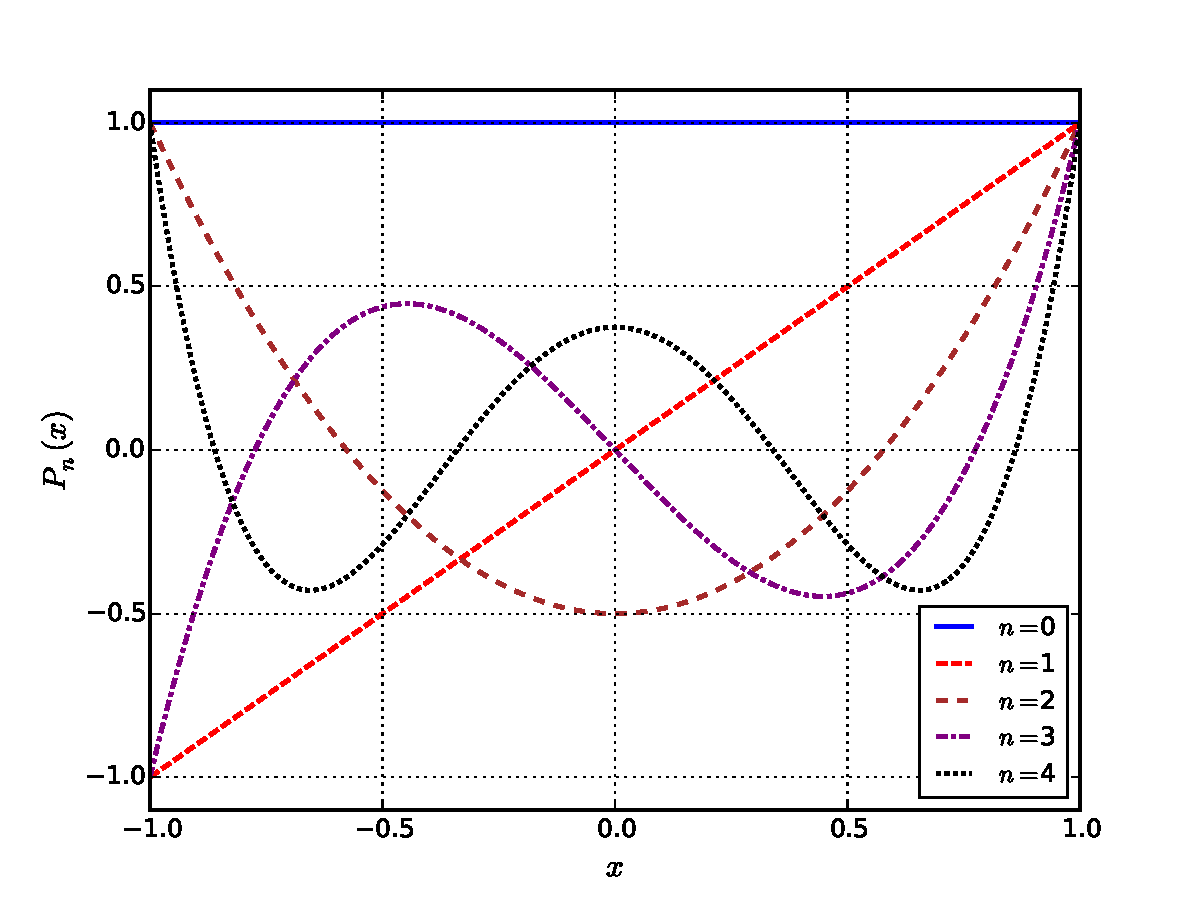
\includegraphics[angle=0,width=0.8\textwidth]{figs/fig-Legendre-P.pdf}
\caption{Primeros cinco polinomios de Legendre. C'odigo Python disponible \href{https://github.com/gfrubi/FM2/blob/master/figuras-editables/fig-Legendre.py}{aqu\'i}.}
\label{fig-Pn}
\end{figure}

\begin{figure}[H]
\centering
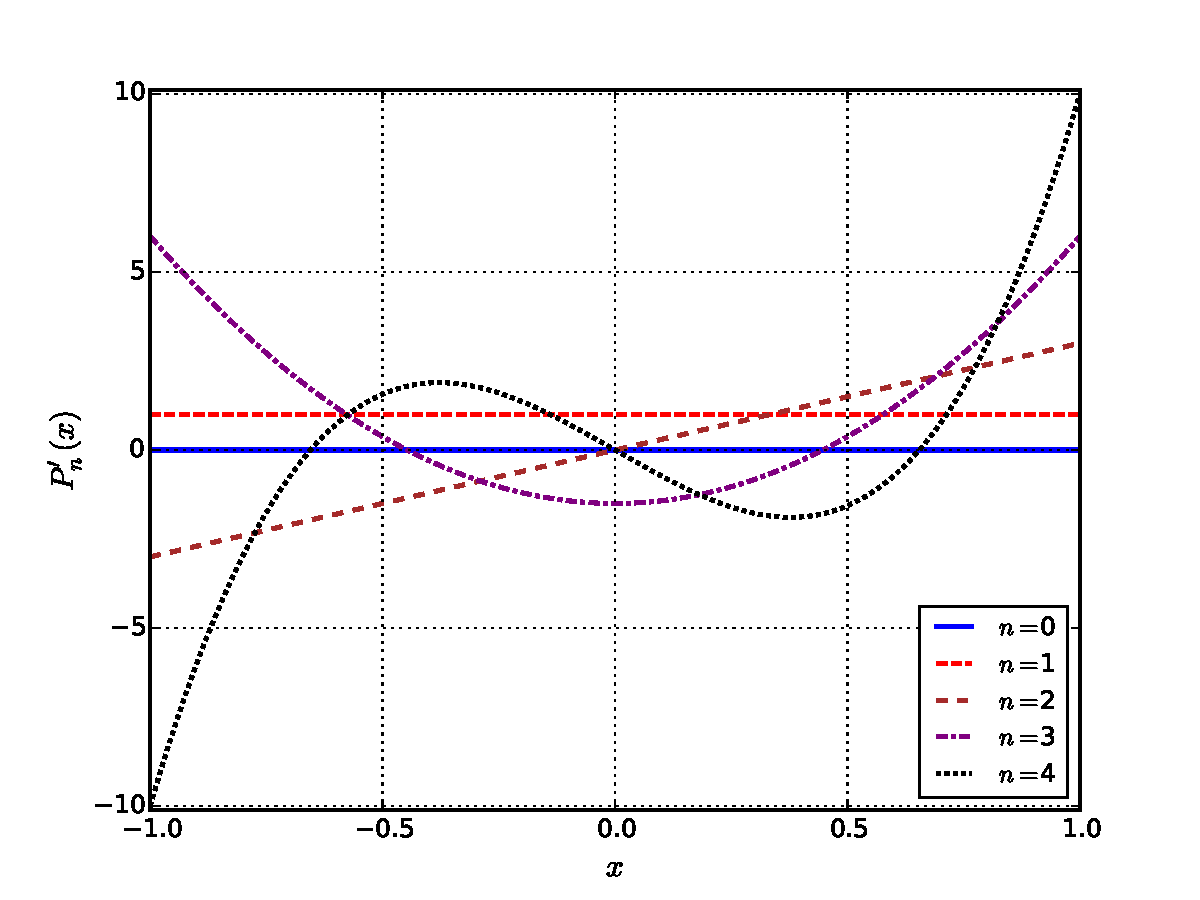
\includegraphics[angle=0,width=0.8\textwidth]{figs/fig-Legendre-der-P.pdf}
\caption{Derivada de los primeros cinco polinomios de Legendre. C'odigo Python disponible \href{https://github.com/gfrubi/FM2/blob/master/figuras-editables/fig-Legendre.py}{aqu\'i}.}
\label{fig-Pnp}
\end{figure}



\subsubsection{F'ormula de Rodrigues}

\begin{equation}
P_{n}(x)=\frac{1}{2^{n}n!}\frac{d^{n}}{dx^{n}}(x^2-1)^{n}
\end{equation}


\subsubsection{Relaciones de recurrencia}
\begin{gather}
nP_{n-1}(x)+(n+1)P_{n+1}(x)=(2n+1)\,x\,P_n(x), \\
(2n+1)P_n(x)=P'_{n+1}(x)-P'_{n-1}(x).
\end{gather}

\subsection{Relaci'on de ortogonalidad}
\begin{equation}
\frac{d\ }{dx}\left[(1 - x^2) P_n' \right]+ n (n + 1) P_n=0, \quad
\frac{d\ }{dx}\left[(1 - x^2) P_m' \right]+ m (m + 1) P_m=0 .
\end{equation}

\begin{gather}
[n (n + 1) - m (m + 1)]\int_{-1}^1 P_n(x) P_m(x)\,d x = 0 
\\
\int_{-1}^1 P_n(x) P_m(x)\,d x = 0, \qquad n\neq m.
\end{gather}
\begin{equation}\label{ortoPn}
\boxed{\int_{-1}^{1}P_n(x)P_m(x)\,dx=\frac{2}{2n+1}\delta_{mn}.}
\end{equation}
Como los polinomios de Legendre son ortogonales, se sigue que son \textit{linealmente independientes} (l.i.), ya que
\begin{equation}
\sum_{n=0}^\infty a_nP_n(x)=0,
\end{equation}
s'i y s'olo si $a_n=0$.
\subsection{Series de Legendre}
Es posible expandir una funci'on $f(x)$, definida en el intervalo $x\in[-1,1]$ y continua por tramos, en una \textbf{serie de Legendre}, es decir, en una suma de polinomios de Legendre, de la forma
\begin{equation}
f(x)=\sum_{n=0}^\infty a_nP_n(x),
\end{equation}
en el sentido que la serie coverge en media a la funci'on $f(x)$ para todo $x$ en $[-1,1]$.

Podemos encontrar una expresi'on para los coeficientes usando la relaci'on de ortogonalidad \eqref{ortoPn}:
\begin{equation}
a_n=\frac{2n+1}{2}\int_{-1}^1 f(x)P_n(x)\,dx.
\end{equation}
\subsubsection{Expansi'on de Legendre de la Delta de Dirac}
En el caso en que $f(x)=\delta(x-a)$ tendremos que
\begin{align}
a_n &= \frac{2n+1}{2}\int_{-1}^1 \delta(x-a)P_n(x)\,dx \\
&= \frac{2n+1}{2}P_n(a),
\end{align}
y entonces
\begin{equation}
\delta(x-a)=\sum_{n=0}^\infty \frac{2n+1}{2}P_n(a)P_n(x).
\end{equation}
En particular, usando \eqref{Pn0} encontramos
\begin{equation}
\delta(x)=\sum_{m=0}^\infty \frac{(-1)^m(4m+1)(2m)!}{2^{2m+1}(m!)^2}P_{2m}(x).
\end{equation}

\begin{figure}[H]
\centering
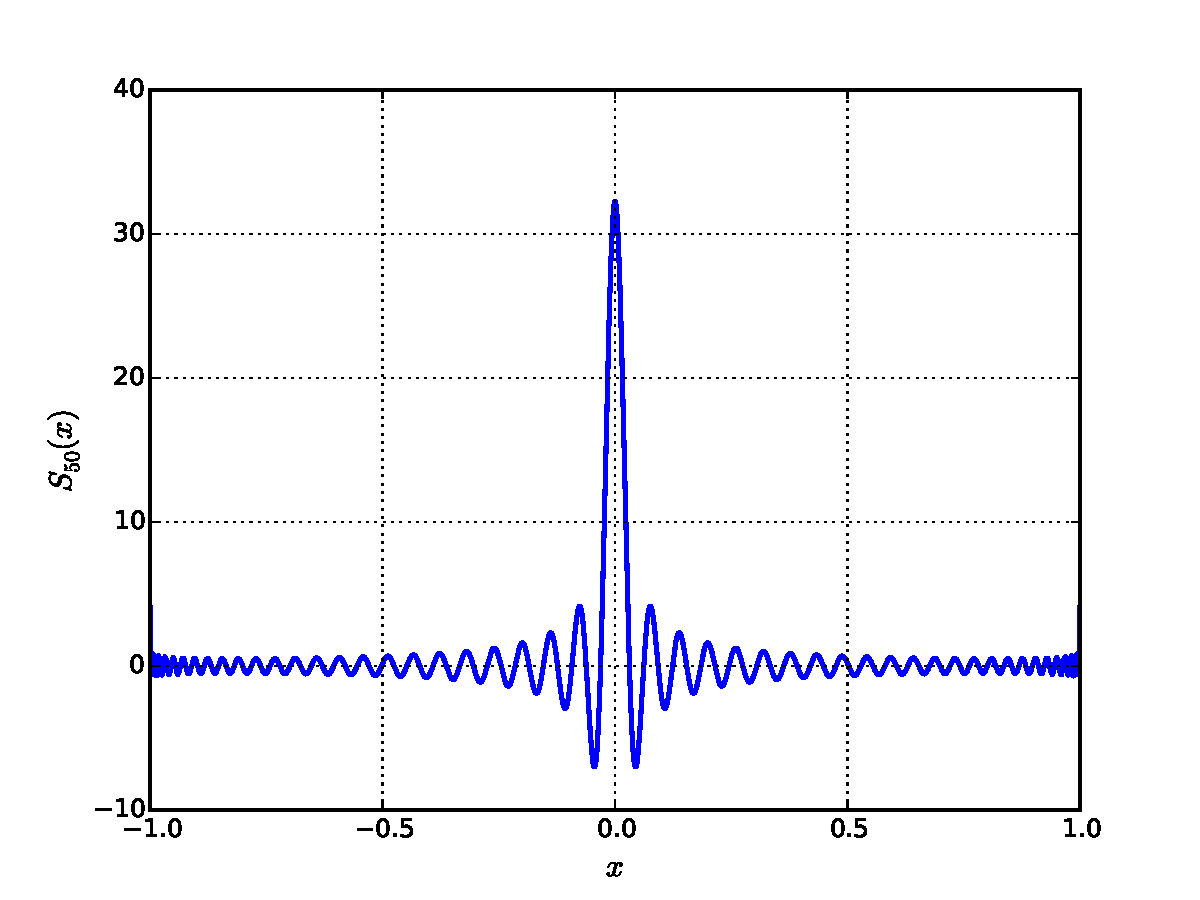
\includegraphics[angle=0,width=0.8\textwidth]{figs/fig-Legendre-serie-Delta.pdf}
\caption{Serie (truncada a orden $50$) de la serie de Legendre de $\delta(x)$.}
\label{fig-DSL}
\end{figure}

\subsection{Soluci'on en serie de Potencias (M'etodo de Frobenius)}\label{sec:FrobLeg}

Primero escribimos la E.D.O. de Legendre \eqref{ecLeg} en su forma estandar:
\begin{equation}
\label{eqn_legendre_eqn}
\left( 1 - x^2 \right) y'' - 2 x y' + Q y = 0,
\end{equation}
o bien
\begin{equation}
\label{eqn_legendre_eqn_norm}
y'' - \frac{2 x}{1 - x^2} y' + \frac{ Q }{1 - x^2} y = 0.
\end{equation}
Como los coeficientes de $y'$ y $y$ son funciones anal'iticas en la vencindad de 
$x = 0$, podemos encontrar una soluci'on en serie de Taylor en torno a ese punto:
\begin{align*}
y &= \sum_{k=0}^\infty a_k x^k ,
\\
y' &= \sum_{k=0}^\infty k a_k x^{k-1} ,
\\
y'' &= \sum_{k=2}^\infty (k-1) k a_k x^{k-2} 
\\
&= \sum_{k=0}^\infty (k+1) (k+2) a_{k+2} x^k.
\end{align*}
Sustituyendo estas series en \eqref{eqn_legendre_eqn} obtenemos
\begin{equation}
\sum_{k=0}^\infty (k+1) (k+2) a_{k+2} x^k
- \sum_{k=0}^\infty (k-1) k a_k x^k
- 2 \sum_{k=0}^\infty k a_k x^k
+ Q \sum_{k=0}^\infty a_k x^k= 0 ,
\end{equation}
\begin{equation}
\sum_{k=0}^\infty \left[ (k+1)(k+2) a_{k+2} - \left( (k-1) k + 2 k - Q \right) a_k \right] x^k = 0.
\end{equation}
Igualando los coeficientes de cada t'ermino $x^k$ obtenemos las relaciones de recurrencia
\begin{equation}\label{recLeg}
a_{k+2} = \frac{ k (k+1) - Q}{ (k+1)(k+2) } a_k, \qquad k=0,1,2,\cdots.
\end{equation}
A partir de ellas, podemos encontrar todos los coeficientes $a_k$, con $k\ge 2$ a partir de $a_0$ y $a_1$:
\begin{equation}
a_k =
\begin{cases}
\displaystyle{
\frac{a_0}{k!} \prod_{\substack{l=0 \\ l \text{ par}}}^{k-2} 
\left( l (l+1) - Q \right),
}
&k \text{ par}, 
\\
\displaystyle{
\frac{a_1}{k!} \prod_{\substack{l=1 \\ l \text{ impar}}}^{k-2} \left( l (l+1) - Q \right),
}
&k \text{ impar} .
\end{cases}
\end{equation}

Por lo tanto, la soluci'on general ser'a una combinaci'on lineal de la forma
\begin{equation}
y(x)=a_0y_1(x)+a_1y_2(x),
\end{equation}
donde $y_1(x)$ es una funci'on par en $x$ e $y_2(x)$ es una funci'on impar en $x$, dadas por
\begin{equation}
y_1(x) = \sum_{m= 0}^\infty \left(\frac{1}{(2m)!}
\prod_{\substack{l=0 \\ l \text{ par}}}^{2m-2}
\left( l (l+1) -Q \right) \right) x^{2m}=:\sum_{m= 0}^\infty b_m x^{2m}, \label{y1}
\end{equation}
\begin{equation}
y_2(x) = \sum_{m=0}^\infty\left( \frac{1}{(2m+1)!}
\prod_{\substack{l=1 \\ l \text{ impar}}}^{2m-1}
\left( l (l+1) - Q \right) \right) x^{2m+1}
=:\sum_{m= 0}^\infty c_m x^{2m+1}. \label{y2}
\end{equation}

En general, tanto $y_1(x)$ como $y_2(x)$ ser'an series infinitas, ya que los correspondientes coeficientes de cada $x^k$, dados por un producto de factores, ser'an no nulos \textit{excepto si existe un valor de $l$ tal que} $l(l+1)-Q=0$. Esto s'olo ocurrir'a si la constante $Q$ es de la forma $Q=n(n+1)$, con alg'un valor de $n=0,1,2,\cdots$. Si este es el caso, entonces una de las series se \textit{truncar'a}, reduci'endose a un polinomio.

\subsubsection{Convergencia}
Analicemos primero el caso gen'erico en que $Q\neq n(n+1)$. Como dijimos, las dos soluciones l.i. $y_1(x)$ e $y_2(x)$ ser'an series infinitas, debiendo por tanto analizar su convergencia.

Consideramos primero el \textbf{test de D'\,Alambert}\footnote{Tambi'en llamado ``Cauchy ratio test'': Si $\lim_{n\to\infty}\left|u_{n+1}/u_n\right|<1$ entonces $\sum_{n=0}^\infty u_n$ es una serie convergente. Si $\lim_{n\to\infty}\left|u_{n+1}/u_n\right|>1$ la serie es divergente. Si $\lim_{n\to\infty}\left|u_{n+1}/u_n\right|=1$ el test de Cauchy no suministra informaci'on. Ver, por ejemplo, \cite{Arfken}, secci'on 5.2.}. Para el caso de $y_1(x)$ tenemos que $y_1(x)=\sum_{m=0}^\infty u_m$, con 
\begin{equation}
u_m=\frac{x^{2m}}{(2m)!}
\prod_{\substack{l=0 \\ l \text{ par}}}^{2m-2}
\left( l (l+1) -Q \right)=a_{2m}x^{2m},
\end{equation}
y entonces
\begin{align}
\lim_{m\to\infty}\left|\frac{u_{m+1}}{u_m}\right| 
&=\lim_{m\to\infty}\left|\frac{b_{m+1}x^{2m+2}}{b_mx^{2m}}\right|
= \lim_{m\to\infty}\left|\frac{a_{2m+2}}{a_{2m}}\right| x^2 \\
&= \lim_{m\to\infty}\left|\frac{(2m(2m+1)-Q)}{(2m+1)(2m+2)}\right| x^2
= x^2.
\end{align}

Por lo tanto, podemos afirmar que $y_1(x)$ es convergente para $|x|<1$. Para analizar la convergencia cuando $x=\pm 1$ podemos usar el test de Gauss\footnote{Si $u_n>0$ $\forall n$ y $u_n/u_{n+1}=1+h/n+B(n)/n^2$ donde $h$ es una constante y $B(n)$ una funci'on acotada de $n$ para $n\to\infty$ entonces la serie $\sum_n u_n$ converge si $h>1$ y diverge si $h\le 1$. Ver, por ejemplo, \cite{Arfken}, secci'on 5.2.}. En nuestro caso ($u_m>0$ para $m$ suficientemente grande) y 
\begin{equation}
\frac{u_m}{u_{m+1}}=\frac{(2m+1)(2m+2)}{(2m(2m+1)-Q)}=\left[1+\frac{1}{m}+\frac{Q}{8m^2}\left(2+\frac{1}{m}+O(\frac{1}{m^2})\right)\right].
\end{equation}
Por lo tanto, $h=1$ y entonces $y_1(x)$ es una serie divergente en $x=\pm 1$.

An'alogamente, puede verificarse que las mismas conclusiones son v'alidas para $y_2(x)$. En resumen, 

\begin{quote}
si $Q\neq n(n+1)$ las soluciones de la ec. de Legendre son divergentes en los extremos del intervalo considerado, e.d. en $x=\pm 1$.
\end{quote}

\subsubsection{Caso $Q=n(n+1)$}
Analicemos ahora con m'as detalle el caso en que $Q=n(n+1)$, puesto que aqu'i obtendremos series truncadas (es decir, polinomios) que naturalmente son funciones finitas en todo el intervalo considerado, incluyendo los extremos. De (\ref{recLeg}) vemos que $a_{n+2}=0$, y por consiguiente todos los coeficientes de orden superior de la forma $a_{n+2p}$ ser'an nulos, con $p=1,2,\cdots$. Por lo tanto, si $n$ es par entonces ser'a la serie $y_1(x)$ la que se truncar'a, mientras que $y_2(x)$ continuar'a siendo una serie infinita. Por otro lado, si $n$ es impar $y_1(x)$ tendr'a infinitos t'erminos, mientras que $y_2(x)$ se reduce a un polinomio. El orden del correspondiente polinomio truncado es $n$ en ambos casos ($a_n$ es el 'ultimo t'ermino no nulo). Esperamos por lo tanto que estos polinomios sean proporcionales a los polinomios de Legendre de orden $n$. A partir de (\ref{y1}) e (\ref{y2}), y usando $l(l+1)-n(n+1)=(l-n)(l+n+1)$ encontramos que
\begin{equation}\label{y1n1}
y_{1,n}(x) = \sum_{m= 0}^{n/2}b_mx^{2m}, \qquad b_m=\frac{1}{(2m)!}
\prod_{\substack{l=0 \\ l \text{ par}}}^{2m-2}
(l-n)(l+n+1), \qquad n\text{ par},
\end{equation}
\begin{equation}\label{y2n1}
y_{2,n}(x)=\sum_{m= 0}^{(n-1)/2}c_mx^{2m+1}, \qquad c_m =\frac{1}{(2m+1)!}
\prod_{\substack{l=1 \\ l \text{ impar}}}^{2m-1}
 (l-n)(l+n+1), \qquad n\text{ impar}.
\end{equation}

Luego de algo de 'algebra, podemos verificar que
\begin{equation}
b_m=\frac{(-1)^m}{(2m)!}\frac{(n+2m)![(n/2)!]^2}{n!(n/2-m)!(n/2+m)!},
\end{equation}
y con ello, podemos escribir la soluci'on $y_{1,n}$ como
\begin{align}
y_{1,n}(x) &= \frac{[(n/2)!]^2}{n!}\sum_{m=0}^{n/2}\frac{(-1)^m}{(2m)!}\frac{(n+2m)!}{(n/2-m)!(n/2+m)!}x^{2m}.
\end{align}
Finalmente, cambiando 'indice de suma desde $m$ hasta $k:=n/2-m$, de modo que $2m=n-2k$, podemos escribir
\begin{align}
y_{1,n}(x) &= \frac{[(n/2)!]^2}{n!}\sum_{k=0}^{n/2}\frac{(-1)^{n/2-k}}{(n-2k)!}\frac{(2n-2k)!}{k!(n-k)!}x^{n-2k} \\
&= (-1)^{n/2}\frac{[(n/2)!]^2}{n!}\sum_{k=0}^{n/2}\frac{(-1)^{k}}{(n-2k)!}\frac{(2n-2k)!}{k!(n-k)!}x^{n-2k} \\
&= (-1)^{n/2}\frac{[(n/2)!]^2}{n!} 2^n P_n(x), \qquad n=0,2,4,\cdots. \label{y1Pn}
\end{align}
En el 'ultimo paso hemos identificado la serie de potencias \eqref{seriePn} de los polonomios de Legendre.

An'alogamente, para $n$ impar podemos expresar los coeficientes $c_m$ como
\begin{equation}
c_m=\frac{(-1)^m}{(2m+1)!}\frac{(n+2m)![\left(\frac{n-1}{2}\right)!]^2}{n!\left(\frac{n-2m-1}{2}\right)!\left(\frac{n+2m-1}{2}\right)!},
\end{equation}
de modo que
\begin{align}
y_{2,n}(x) &= \sum_{m=0}^{(n-1)/2}\frac{(-1)^m}{(2m+1)!}\frac{(n+2m)![\left(\frac{n-1}{2}\right)!]^2}{n!\left(\frac{n-2m-1}{2}\right)!\left(\frac{n+2m-1}{2}\right)!}x^{2m+1} \\
&= \frac{[\left(\frac{n-1}{2}\right)!]^2}{n!}\sum_{m=0}^{(n-1)/2}\frac{(-1)^m}{(2m+1)!}\frac{(n+2m)!}{\left(\frac{n-2m-1}{2}\right)!\left(\frac{n+2m-1}{2}\right)!}x^{2m+1}
\end{align}
Cambiamos ahora 'indice de suma, definiendo $k$ tal que $2m+1=n-2k$, y encontramos
\begin{align}
y_{2,n}(x) &= \frac{[n/2]!^2}{n!}\sum_{k=0}^{(n-1)/2}\frac{(-1)^{\frac{n-2k-1}{2}}}{(n-2k)!}\frac{(2n-2k-1)!}{k!(n-k-1)!}\,x^{n-2k} \\
&= \frac{[n/2]!^2}{n!}(-1)^{(n-1)/2}\sum_{k=0}^{[n/2]}\frac{(-1)^k}{(n-2k)!}\frac{(2n-2k)!}{(2n-2k)}\frac{1}{k!}\frac{(n-k)}{(n-k)!}\,x^{n-2k} \\
&= \frac{[n/2]!^2}{n!}\frac{(-1)^{[n/2]}}{2}\sum_{k=0}^{[n/2]}\frac{(-1)^k}{(n-2k)!}\frac{(2n-2k)!}{k!(n-k)!}\,x^{n-2k} \\
&= \frac{[n/2]!^2}{n!}(-1)^{[n/2]}2^{n-1} P_n(x), \qquad n=1,3,5,\cdots. \label{y2Pn}
\end{align}
En resumen, usando una notaci'on algo m'as compacta, podemos escribir:
\begin{equation}
P_n(x):=(-1)^{[n/2]}2^{-2[n/2]}\frac{n!}{[n/2]!^2} \times
	\begin{cases}
	y_{1,n}(x) , & n \text{ par}\\
	y_{2,n}(x), & n \text{ impar}.
	\end{cases}
\end{equation}

\subsection{Funciones de Legendre de segunda especie}
Como hemos visto, en el caso en que $Q=n(n+1)$ una de las series ($y_1$ si $n$ es par, $y_2$ si $n$ es impar) se trunca, reduci'endose (salvo factores constantes) a los polinomios de Legendre. Por lo tanto, para cada $n$, existe una segunda soluci'on de la ec. de Legendre, que quedaa expresada como serie infinita, que convergen para $x\in(-1,1)$ pero diverge en $x=\pm 1$. Estas funciones son llamadas las \textbf{funciones de Legendre de segunda especie}, $Q_n(x)$, que por conveniencia definiremos usando factores an'alogos a aquellos encontrados en \eqref{y1Pn} y \eqref{y1Pn}:
\begin{equation}
Q_n(x):=
	\begin{cases}
	(-1)^{n/2}\frac{[(n/2)!]^2}{n!} 2^n\, y_{2,n}(x), & n \text{ par}\\
	(-1)^{(n+1)/2}\frac{\left[\left(\frac{n-1}{2}\right)!\right]^2}{n!}2^{n-1}\, y_{1,n}(x), & n \text{ impar}.
	\end{cases} \label{Q_n}
\end{equation}

\subsubsection{Relaciones de Recurrencia}
A partir de las definiciones \eqref{Q_n} es posible verificar la siguiente importante propiedad: 
\begin{quote}
\textit{Las funciones de Legendre de segunda especie satisfacen las mismas relaciones de recurrencia que los polinomios de Legendre}.
\end{quote} 

Como consecuencia, \textit{todas} las relaciones de recurrencia que derivamos para los polinomios de Legendre son v'alidas para las correspondientes funciones de segunda especie. Podemos verificar nuevamente a partir de estas identidades que cada $Q_n(x)$ satisface la E.D.O. de Legendre.

En particular, se demostrar'an las siguientes relaciones (a partir de las cuales pueden derivarse todas las otras):
\begin{gather}
nQ_{n-1}(x)+(n+1)Q_{n+1}(x)=(2n+1)\,x\,Q_n(x) , \label{nQn-1}\\
(2n+1)Q_n(x)=Q'_{n+1}(x)-Q'_{n-1}(x).
\end{gather}

En este caso, las soluciones adoptan la forma (ver \eqref{y1} y \eqref{y1}, comparar con \eqref{y1n1} y \eqref{y2n1}):
\begin{equation}\label{y1n}
y_{1,n}(x) = \sum_{m= 0}^{+\infty}b_mx^{2m}, \qquad b_m=\frac{1}{(2m)!}
\prod_{\substack{l=0 \\ l \text{ par}}}^{2m-2}
(l-n)(l+n+1), \qquad b_0=1,  
\end{equation}
\begin{equation}\label{y2n}
y_{2,n}(x)=\sum_{m= 0}^{+\infty}c_mx^{2m+1}, \qquad c_m=\frac{1}{(2m+1)!}
\prod_{\substack{l=1 \\ l \text{ impar}}}^{2m-1}
 (l-n)(l+n+1), \qquad c_0=1.
\end{equation}
A partir de las definiciones en (\ref{Q_n}), podemos escribir:
%\begin{equation}
%xQ_n(x):=
%	\begin{cases}
%	(-1)^{\frac{n}{2}}\frac{[(n/2)!]^2}{n!} 2^n\,xy_{2,n}(x), & n \text{ par}\\
%	(-1)^{\frac{n+1}{2}}\frac{\left[\left(\frac{n-1}{2}\right)!\right]^2}{n!}2^{n-1}\, xy_{1,n}(x), & n \text{ impar},
%	\end{cases} 
%\end{equation}
\begin{equation}
Q_{n-1}(x):=
	\begin{cases}
	(-1)^{\frac{n}{2}}\frac{[(\frac{n-2}{2})!]^2}{(n-1)!} 2^{n-2} \, y_{1,n-1}(x), & n \text{ par}\\
	(-1)^{\frac{n-1}{2}}\frac{\left[\left(\frac{n-1}{2}\right)!\right]^2}{(n-1)!}2^{n-1}\, y_{2,n-1}(x), & n \text{ impar},
	\end{cases} \label{Q_n-1}
\end{equation}
\begin{equation}
Q_{n+1}(x):=
	\begin{cases}
	(-1)^{\frac{n+2}{2}}\frac{[(\frac{n}{2})!]^2}{(n+1)!} 2^{n} \, y_{1,n+1}(x), & n \text{ par}\\
	(-1)^{\frac{n+1}{2}}\frac{\left[\left(\frac{n+1}{2}\right)!\right]^2}{(n+1)!}2^{n+1}\, y_{2,n+1}(x), & n \text{ impar}.
	\end{cases} \label{Q_n+1}
\end{equation}
Por lo tanto,
\begin{align}
nQ_{n-1}(x) &+ (n+1)Q_{n+1}(x) \nonumber \\
&=\begin{cases}
	(-1)^{\frac{n}{2}}\frac{[(\frac{n}{2})!]^2}{(n)!} 2^{n} \, \left[ y_{1,n-1}(x)-y_{1,n+1} \right], & n \text{ par}\\
	(-1)^{\frac{n+1}{2}}\frac{\left[\left(\frac{n-1}{2}\right)!\right]^2}{(n)!}2^{n-1}\,\left[ -n^2y_{2,n-1}(x)+(n+1)^2y_{2,n+1} \right] , & n \text{ impar}.
	\end{cases} \label{rel.QQ}
\end{align}

Para evaluar el lado derecho de \eqref{rel.QQ} usamos las expresiones en serie \eqref{y1n} y \eqref{y2n}. Para $y_{1,n}(x)$ tenemos que
\begin{eqnarray}
y_{1,n-1}(x)&=&\sum_{m= 0}^{+\infty}\frac{1}{(2m)!}
\prod_{\substack{l=0 \\ l \text{ par}}}^{2m-2}
(l-n+1)(l+n)\,x^{2m} ,\\
y_{1,n+1}(x)&=&\sum_{m= 0}^{+\infty}\frac{1}{(2m)!}
\prod_{\substack{l=0 \\ l \text{ par}}}^{2m-2}
(l-n-1)(l+n+2)\,x^{2m}.
\end{eqnarray}
Reescribimos ahora ambas expresiones como
\begin{equation}\label{pit1}
y_{1,n-1}(x)=\sum_{m= 0}^{+\infty}\frac{1}{(2m)!}
\prod_{\substack{l=1 \\ l \text{ impar}}}^{2m-1} 
(l-n)(l+n-1)\,x^{2m},
\end{equation}
\begin{equation}
y_{1,n+1}(x)=\sum_{m= 0}^{+\infty}\frac{1}{(2m)!}
\prod_{\substack{l=1 \\ l \text{ impar}}}^{2m-1}
(l-n-2)(l+n+1)\,x^{2m}. \label{pit2}
\end{equation}
Luego, ya que
\begin{eqnarray}
\prod_{\substack{l=1 \\ l \text{ impar}}}^{2m-1}(l+n-1)&=&n\prod_{\substack{l=3 \\ l \text{ impar}}}^{2m-1}(l+n-1)=n\prod_{\substack{l=1 \\ l \text{ impar}}}^{2m-3}(l+n+1),\\
\prod_{\substack{l=1 \\ l \text{ impar}}}^{2m-1}(l-n-2)&=&-(n+1)\prod_{\substack{l=3 \\ l \text{ impar}}}^{2m-1}(k-n-2)=-(n+1)\prod_{\substack{l=1 \\ l \text{ impar}}}^{2m-3}(l-n),
\end{eqnarray}
tenemos que \eqref{pit1} y \eqref{pit2} son equivalentes a:
\begin{equation}
y_{1,n-1}(x)=n\sum_{m= 0}^{+\infty}\frac{1}{(2m)!}
\prod_{\substack{l=1 \\ l \text{ impar}}}^{2m-3} 
(l+n+1)(l-n)(2m-1-n)\,x^{2m},
\end{equation}
\begin{equation}
y_{1,n+1}(x)=-(n+1)\sum_{m= 0}^{+\infty}\frac{1}{(2m)!}
\prod_{\substack{l=1 \\ l \text{ impar}}}^{2m-1}
(l-n)(l+n+1)(2l+n)\,x^{2m}.
\end{equation}
Entonces, 
\begin{eqnarray}
y_{1,n-1}(x)-y_{1,n+1}(x)&=&(2n+1)\sum_{m= 1}^{+\infty}\frac{1}{(2m-1)!}
\prod_{\substack{l=1 \\ l \text{ impar}}}^{2m-3}
(l-n)(l+n+1)\,x^{2m}\\
&=& (2n+1)\sum_{m= 0}^{+\infty}\frac{1}{(2m+1)!}
\prod_{\substack{l=1 \\ l \text{ impar}}}^{2m-1}
(l-n)(l+n+1)\,x^{2m+2}\\
&=& (2n+1)\,x\,y_{2,n}(x) .\label{uno}
\end{eqnarray}

%\begin{equation}
%y_{2,n}=\sum_{m= 0}^{+\infty}\frac{1}{(2m+1)!}
%\prod_{\substack{l=1 \\ l \text{ impar}}}^{2m-1}
% (l-n)(l+n+1)x^{2m+1}
%\end{equation}

Por otro lado, de la expresi\'on en serie \eqref{y2n} para $y_{2,n}(x)$, y  siguiendo el mismo reci'en empleado, tenemos que
\begin{eqnarray}
y_{2,n+1}(x)&=&\sum_{m= 0}^{+\infty}\frac{1}{(2m+1)!}
\prod_{\substack{l=1 \\ l \text{ impar}}}^{2m-1}
(l-n-1)(l+n+2)x^{2m+1}\\
&=&\sum_{m= 0}^{+\infty}\frac{1}{(2m+1)!}
\prod_{\substack{l=1 \\ l \text{ par}}}^{2m-2}
(l-n)(l+n+3)x^{2m+1}\\
&=&\frac{1}{n+1}\sum_{m= 0}^{+\infty}\frac{(2m+n+1)}{(2m+1)!}
\prod_{\substack{l=0 \\ l \text{ par}}}^{2m-2}
(l-n)(l+n+1)x^{2m+1}. \label{qn+1}
\end{eqnarray}
Similarmente, 
\begin{eqnarray}
y_{2,n-1}(x)&=&\sum_{m= 0}^{+\infty}\frac{1}{(2m+1)!}
\prod_{\substack{l=1 \\ l \text{ impar}}}^{2m-1}
 (l-n+1)(l+n)x^{2m+1}\\
&=&\sum_{m= 0}^{+\infty}\frac{1}{(2m+1)!}
\prod_{\substack{l=0 \\ l \text{ par}}}^{2m-2}
 (l-n+2)(l+n+1)x^{2m+1}\\
 &=&-\frac{1}{n}\sum_{m= 0}^{+\infty}\frac{(2m-n)}{(2m+1)!}
\prod_{\substack{l=0 \\ l \text{ par}}}^{2m-2}
 (l-n)(l+n+1)x^{2m+1}. \label{qn-1}
\end{eqnarray}

De este modo, usando \eqref{qn+1} y \eqref{qn-1}, encontramos que
\begin{eqnarray}
(n+1)^2y_{2,n+1}(x)-n^2y_{2,n+1}(x)&=&(2n+1)\sum_{m= 0}^{+\infty}\frac{1}{(2m)!}
\prod_{\substack{l=0 \\ l \text{ par}}}^{2m-2}
 (l-n)(l+n+1)x^{2m+1} \\
 &=&(2n+1)\,x\,y_{1,n}(x). \label{dos}
\end{eqnarray}

Finalmente, reemplazamos \eqref{uno} y \eqref{dos} en \eqref{rel.QQ}, y obtenemos
\begin{eqnarray}
nQ_{n-1}(x)+(n-1)Q_{n+1}(x) &=&
   \begin{cases}
	(-1)^{\frac{n}{2}}\frac{[(\frac{n}{2})!]^2}{(n)!} 2^{n} \,(2n+1)xy_{2,n}(x), & n \text{ par}\\
	(-1)^{\frac{n+1}{2}}\frac{\left[\left(\frac{n-1}{2}\right)!\right]^2}{(n)!}2^{n-1}\, (2n+1)\,x\,y_{1,n}(x), & n \text{ impar}
	\end{cases}\\ 
	&=&(2n+1)\,x
   \begin{cases}
	(-1)^{\frac{n}{2}}\frac{[(\frac{n}{2})!]^2}{(n)!} 2^{n} \,y_{2,n}(x), & n \text{ par}\\
	(-1)^{\frac{n+1}{2}}\frac{\left[\left(\frac{n-1}{2}\right)!\right]^2}{(n)!}2^{n-1}\,y_{1,n}(x), & n \text{ impar}
	\end{cases} \\
	&=&  (2n+1)\,x\,Q_n(x),
\end{eqnarray}
demostrando as'i la identidad \eqref{nQn-1}.


Para demostrar la segunda relaci\'on de recurrencia, \eqref{nQn-1}, calculamos:
\begin{align}
Q'_{n+1}(x) &- Q'_{n-1}(x) \\
&=\begin{cases}
	(-1)^{\frac{n}{2}}\frac{[(\frac{n}{2})!]^2}{(n)!} 2^{n} \, \left[ -\frac{1}{n+1}y'_{1,n+1}(x)-\frac{1}{n}y'_{1,n-1} \right], & n \text{ par}\\
	(-1)^{\frac{n+1}{2}}\frac{\left[\left(\frac{n-1}{2}\right)!\right]^2}{(n)!}2^{n-1}\,\left[ (n+1)y'_{2,n+1}(x)+ny'_{2,n-1} \right] , & n \text{ impar}.
	\end{cases} \label{q'}
\end{align}
Usamos nuevamente las expresiones en serie de las funciones $y_{1,n}(x)$, y entonces
\begin{eqnarray}
y'_{1,n+1}(x)&=&\sum_{m= 1}^{+\infty}\frac{1}{(2m-1)!}
\prod_{\substack{l=0 \\ l \text{ par}}}^{2m-2}
(l-n-1)(l+n+2)\,x^{2m-1} \\
&=&\sum_{m= 0}^{+\infty}\frac{1}{(2m+1)!}
\prod_{\substack{l=0 \\ l \text{ par}}}^{2m}
(l-n-1)(l+n+2)\,x^{2m+1} \\
&=&-(n+1)\sum_{m= 0}^{+\infty}\frac{2m+n+2}{(2m+1)!}
\prod_{\substack{l=1 \\ l \text{ impar}}}^{2m-1}
(l-n)(l+n+1)\,x^{2m+1}. \label{y'n+1}
\end{eqnarray}
An'alogamente,
\begin{eqnarray}
y'_{1,n-1}(x)&=&\sum_{m= 1}^{+\infty}\frac{1}{(2m-1)!}
\prod_{\substack{l=0 \\ l \text{ par}}}^{2m-2}
(l-n+1)(l+n)\,x^{2m-1} \\
&=&\sum_{m= 0}^{+\infty}\frac{1}{(2m+1)!}
\prod_{\substack{l=0 \\ l \text{ par}}}^{2m}
(l-n+1)(l+n)\,x^{2m+1} \\
&=&n\sum_{m= 0}^{+\infty}\frac{(2m-n+1)}{(2m-1)!}
\prod_{\substack{l=1 \\ l \text{ impar}}}^{2m+1}
(l-n)(l+n+1)\,x^{2m+1}. \label{y'n-1}
\end{eqnarray}
A partir de \eqref{y'n+1} y \eqref{y'n-1} podemos escribir
\begin{eqnarray}
-\frac{1}{(n+1)}y'_{1,n+1}(x)-\frac{1}{n}y'_{1,n-1}&=&\sum_{m= 0}^{+\infty}\frac{(2n+1)}{(2m+1)!}
\prod_{\substack{l=1 \\ l \text{ impar}}}^{2m-1}
(l-n)(l+n+1)\,x^{2m+1}\\
&=&(2n+1)\,y_{2,n}(x). \label{2n-1y2}
\end{eqnarray}

Por otro lado,
\begin{eqnarray}
y'_{2,n+1}(x)&=&\sum_{m= 0}^{+\infty}\frac{1}{(2m)!}
\prod_{\substack{l=1 \\ l \text{ impar}}}^{2m-1}
(l-n-1)(l+n+2)\,x^{2m} \\
&=&\frac{1}{n+1}\sum_{m= 0}^{+\infty}\frac{(2p+n+1)}{(2m)!}
\prod_{\substack{l=0 \\ l \text{ par}}}^{2m-2}
(l-n)(l+n+1)\,x^{2m}, \label{y2'n+1}
\end{eqnarray}
y similarmente, 
\begin{eqnarray}
y'_{2,n-1}(x)&=&\sum_{m= 0}^{+\infty}\frac{1}{(2m)!}
\prod_{\substack{l=1 \\ l \text{ impar}}}^{2m-1}
(l-n+1)(l+n)\,x^{2m} \\
&=&-\frac{1}{n}\sum_{m= 0}^{+\infty}\frac{(2p-n)}{(2m)!}
\prod_{\substack{l=0 \\ l \text{ par}}}^{2m-2}
(l-n)(l+n+1)\,x^{2m}. \label{y2'n-1}
\end{eqnarray}

Adem'as, \eqref{y2'n+1} y \eqref{y2'n-1} implican que
\begin{eqnarray}
(n+1)y'_{2,n+1}(x)+ny'_{2,n-1}(x)&=&\sum_{m= 0}^{+\infty}\frac{(2n+1)}{(2m)!}
\prod_{\substack{l=0 \\ l \text{ par}}}^{2m-2}
(l-n)(l+n+1)\,x^{2m}\\
&=&(2n+1)\,y_{1,n}(x) \label{2n-1y3}
\end{eqnarray}

Finalmente, reemplazando \eqref{2n-1y2} y \eqref{2n-1y3} en \eqref{q'} llegamos a
\begin{eqnarray}
Q'_{n+1}(x) - Q'_{n-1}(x)&=& 
\begin{cases}
	(-1)^{\frac{n}{2}}\frac{[(\frac{n}{2})!]^2}{(n)!} 2^{n} \,(2n+1)\,y_{2,n}(x) , & n \text{ par}\\
	(-1)^{\frac{n+1}{2}}\frac{\left[\left(\frac{n-1}{2}\right)!\right]^2}{(n)!}2^{n-1}\,(2n+1)\,y_{1,n}(x) , & n \text{ impar}
	\end{cases} \\  
	&=&(2n+1)Q_{n}(x),
\end{eqnarray}
que es precisamente la segunda relaci\'on de recurrencia \eqref{nQn-1}.

\subsubsection{Expresiones expl'icitas para $Q_n(x)$}

Afortunadamente, es posible encontrar expresiones para las funciones $Q_n(x)$ en t'erminos de funciones conocidas. Para esto, primero calculamos $Q_0(x)$:
\begin{equation}
Q_0(x)=y_{2,0}(x)=\sum_{m=0}^\infty\frac{1}{(2m+1)!}
\prod_{\substack{l=1 \\ l \text{ impar}}}^{2m-1}l(l+1)\,x^{2m+1},
\end{equation}

Pero,
\begin{equation}
\prod_{\substack{l=1 \\ l \text{ impar}}}^{2m-1}l(l+1)=1\cdot 2\cdot 3\cdot 4\cdots (2m-1)(2m)=(2m)!.
\end{equation}

Por lo tanto, 
\begin{equation}
Q_0(x)=\sum_{m=0}^\infty\frac{(2m)!}{(2m+1)!}x^{2m+1} =\sum_{m=0}^\infty\frac{x^{2m+1}}{(2m+1)}.
\end{equation}
Esta serie es conocida, ya que vimos que
\begin{equation}
\ln\left(\frac{1+x}{1-x}\right)=2\sum_{m=0}^\infty\frac{x^{2m+1}}{(2m+1)},
\end{equation}
y con esto encontramos finalmente que

\begin{equation}
\boxed{Q_0(x)=\frac{1}{2}\ln\left(\frac{1+x}{1-x}\right).}
\end{equation}

An'alogamente, para $n=1$ tenemos que
\begin{equation}
Q_1(x)=-y_{1,1}(x)=\sum_{m=0}^\infty\frac{1}{(2m)!}
\prod_{\substack{l=0 \\ l \text{ par}}}^{2m-2}(l-1)(l+2)\,x^{2m},
\end{equation}
En este caso, el producto puede escribirse como
\begin{equation}
\prod_{\substack{l=0 \\ l \text{ par}}}^{2m-2}(l-1)(l+2)=-1\cdot 2\cdot 1\cdot 4\cdot 3\cdots (2m-5)(2m-2)(2m-3)(2m)=-\frac{(2m)!}{2m-1}.
\end{equation}
Entonces,
\begin{align}
Q_1(x) &= \sum_{m=0}^\infty\frac{x^{2m}}{(2m-1)} =-1+\sum_{m=1}^\infty\frac{x^{2m}}{(2m-1)} \\
&= -1+\sum_{n=0}^\infty\frac{x^{2n+2}}{(2n+1)}
=-1+x\sum_{n=0}^\infty\frac{x^{2n+1}}{(2n+1)}.
\end{align}
Por lo tanto,
\begin{equation}
\boxed{Q_1(x)=\frac{x}{2}\ln\left(\frac{1+x}{1-x}\right)-1.}
\end{equation}

Conociendo $Q_0(x)$ y $Q_1(x)$ podemos encontrar expresiones para las funciones de $Q_n(x)$ de orden superior usando las relaciones de recurrencia \eqref{nQn-1}, ya que
\begin{equation}
Q_{n+1}(x)=\frac{1}{(n+1)}\left[(2n+1)xQ_n(x)-nQ_{n-1}(x)\right].
\end{equation} 

Por ejemplo,
\begin{align}
Q_2(x) &= \frac{1}{2}\left[3xQ_1(x)-Q_0(x)\right] \\
&= \frac{1}{2}\left[-3x+\frac{3}{2}x^2\ln\left(\frac{1+x}{1-x}\right)-\frac{1}{2}\ln\left(\frac{1+x}{1-x}\right)\right] \\
&= -\frac{1}{4}(1-3x^2)\ln\left(\frac{1+x}{1-x}\right) -\frac{3}{2}x.
\end{align}
An'alogamente, encontramos que
\begin{equation}
Q_3(x)=\frac{1}{4}(5x^3-3x)\ln\left(\frac{1+x}{1-x}\right)-\frac{5}{2}x^2+\frac{2}{3}.
\end{equation}
\begin{figure}[H]
\centering
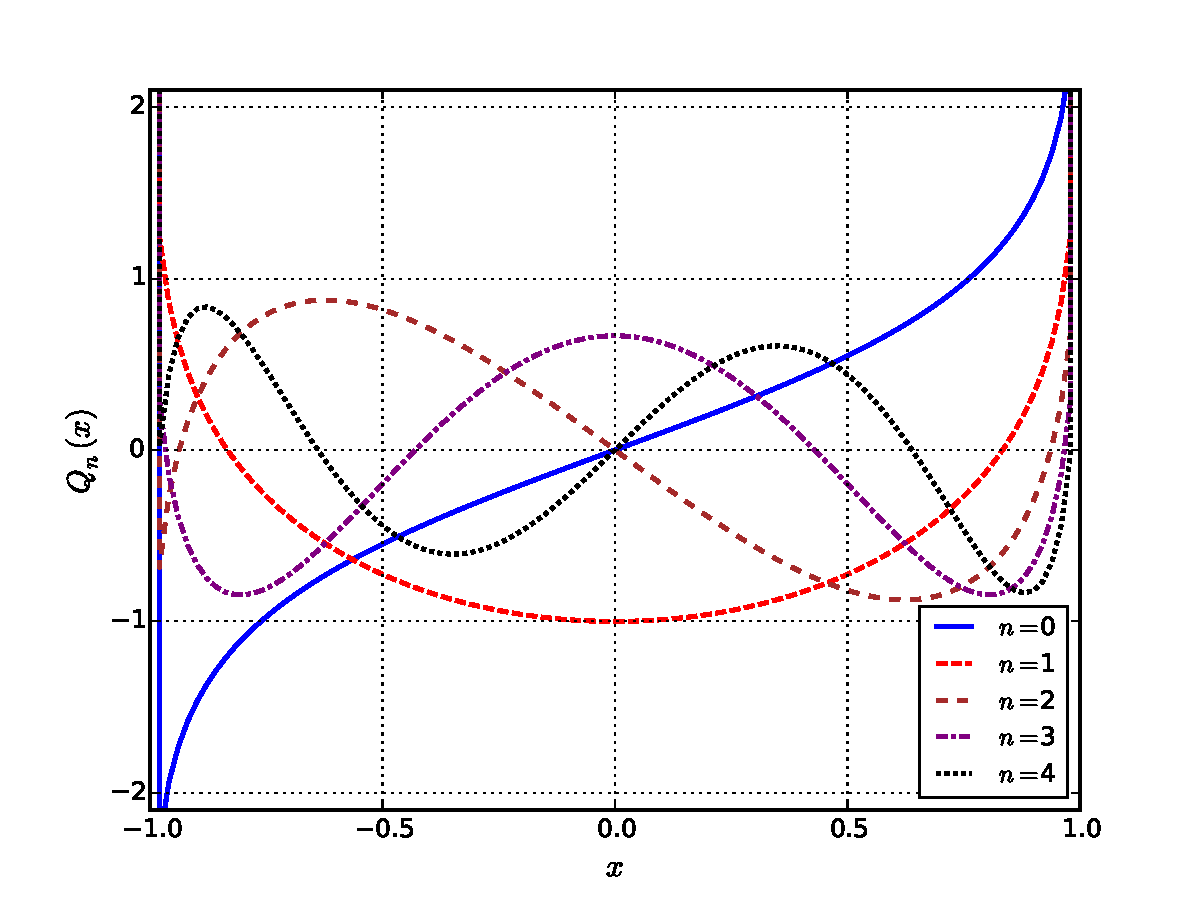
\includegraphics[angle=0,width=0.8\textwidth]{figs/fig-Legendre-Q.pdf}
\caption{Primeras cinco funciones de Legendre de segunda especie.}
\label{fig-Qn}
\end{figure}

\subsubsection{Propiedades de las funciones $Q_n(x)$}
\begin{itemize}
\item Paridad:
\begin{equation}
Q_n(-x)=(-1)^{n+1}Q_n(x)
\end{equation}

\item Valor en el origen:
\begin{equation}
Q_n(0)=
\begin{cases}
0, &  n\text{ par} \\
(-1)^{(n+1)/2}\frac{\left[\left(\frac{n-1}{2}\right)!\right]^2}{n!}2^{n-1}, & n\text{ impar}.
\end{cases}
\end{equation}

\item Valor en extremo del intervalo:
\begin{equation}
\lim_{x\to 1}Q_n(x)=+\infty .
\end{equation}
\end{itemize}



\section{Funciones asociadas de Legendre}

Podemos construir soluciones para la ecuaci'on \eqref{est22} a partir del siguiente teorema:
\begin{quote}
Si $P_Q^m(x)$ es una soluci'on de \eqref{est22} para un valor de $Q$ y $m$ datos, entonces 
\begin{equation}
u(x):=(1-x^2)^{(m+1)/2}\frac{d\ }{dx}\left[(1-x^2)^{-m/2}P_Q^m(x)\right]
\end{equation}
es tambi'en soluci'on de \eqref{est22}, pero con $m+1$ en lugar de $m$.
\end{quote}
Este resultado permite entonces generar nuevas soluciones, con distintos valores de $m$, a partir de una soluci'on conocida, y en particular a partir de $P_n^0$ que definimos como los polinomios de Legendre, $P_n^0(x):=P_n(x)$. A partir de esto, podemos definir las funciones asociadas de Legendre $P_n^m$ tales que
\begin{equation}\label{Pnm+1}
P_n^{m+1}(x)=(1-x^2)^{(m+1)/2}\frac{d\ }{dx}\left[(1-x^2)^{-m/2}P_n^m(x)\right]
\end{equation}
Iterando la relaci'on \eqref{Pnm+1} obtenemos, para $m=0,1,2,\cdots$, 
\begin{eqnarray}\label{Pnm}
P_n^m(x) =(1-x^2)^{m/2}\frac{d^m}{dx^m} P_n(x).
\end{eqnarray}
Por otro lado, las funciones con $m$ negativo pueden calcularse usando
\begin{eqnarray}
P_n^{-m}(x) = (-1)^m\frac{(n-m)!}{(n+m)!} P_n^m(x), \qquad m=0,1,2,\cdots.
\label{est29}
\end{eqnarray}

Ya que las funciones $P_n(x)$ son polinomios de orden $n$, vemos que existen soluciones $P_n^m(x)$ no nulas s'olo si
\begin{equation}
  m=0,\pm 1,\pm 2,\cdots,\pm n \qquad\Leftrightarrow\qquad
  |m|\leq n.
\end{equation}
Es decir, existen $2n+1$ valores permitidos de $m$ para cada $n=0,1,2,\cdots$.

\subsection{Expresiones expl'icitas}
\begin{align}
P_1^1(x) &= (1-x^2)^{1/2}, \\
P_2^1(x) &= 3x(1-x^2)^{1/2}, \\
P_2^2(x) &= 3(1-x^2), \\
P_3^1(x) &= \frac{3}{2}(1-x^2)^{1/2}(5x^2-1), \\
P_3^2(x) &= 15(1-x^2)x, \\
P_3^3(x) &= 15(1-x^2)^{3/2}. \\
\end{align}

\begin{figure}[H]
\centering
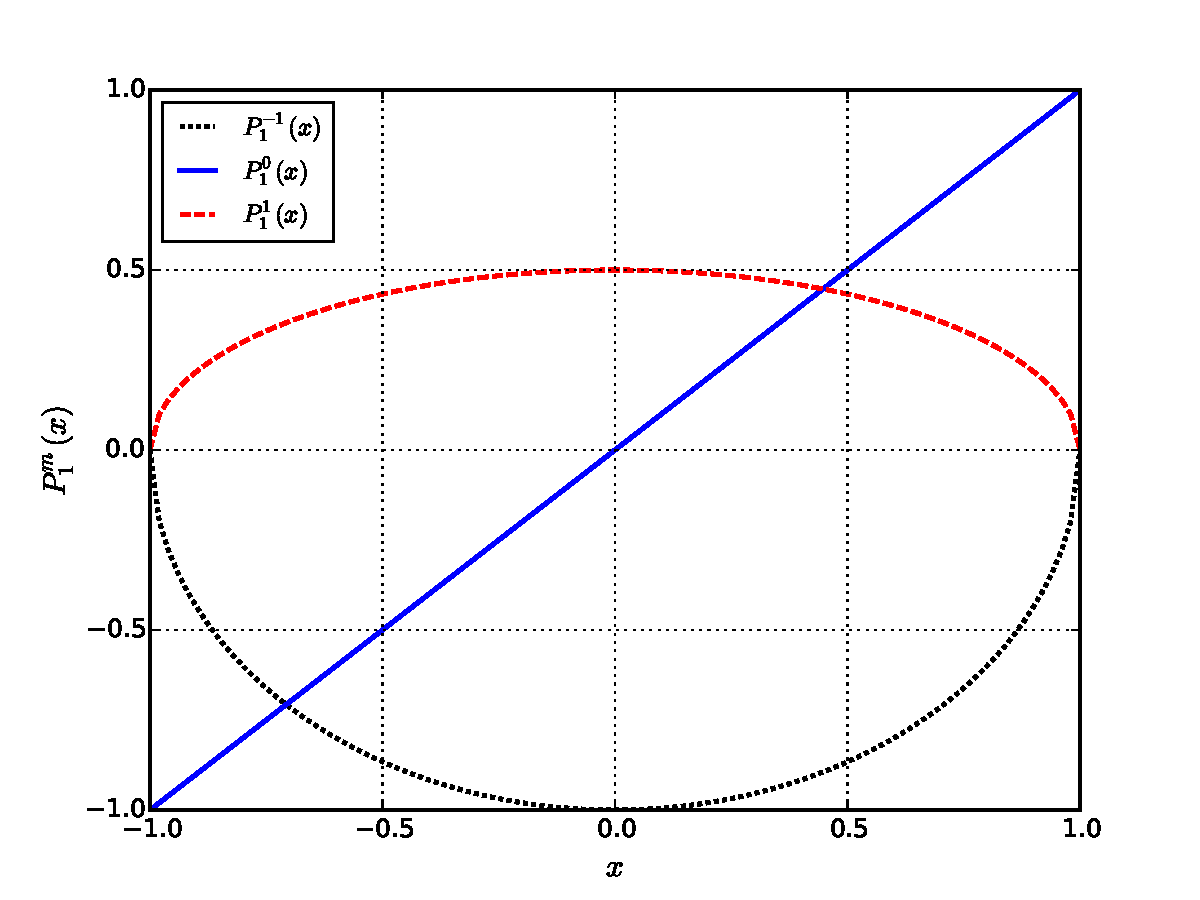
\includegraphics[angle=0,width=0.8\textwidth]{figs/fig-Legendre-Asoc-l-1.pdf}
\caption{Funciones Asociadas de Legendre: $n=1$.}
\label{fig-P1m}
\end{figure}
\begin{figure}[H]
\centering
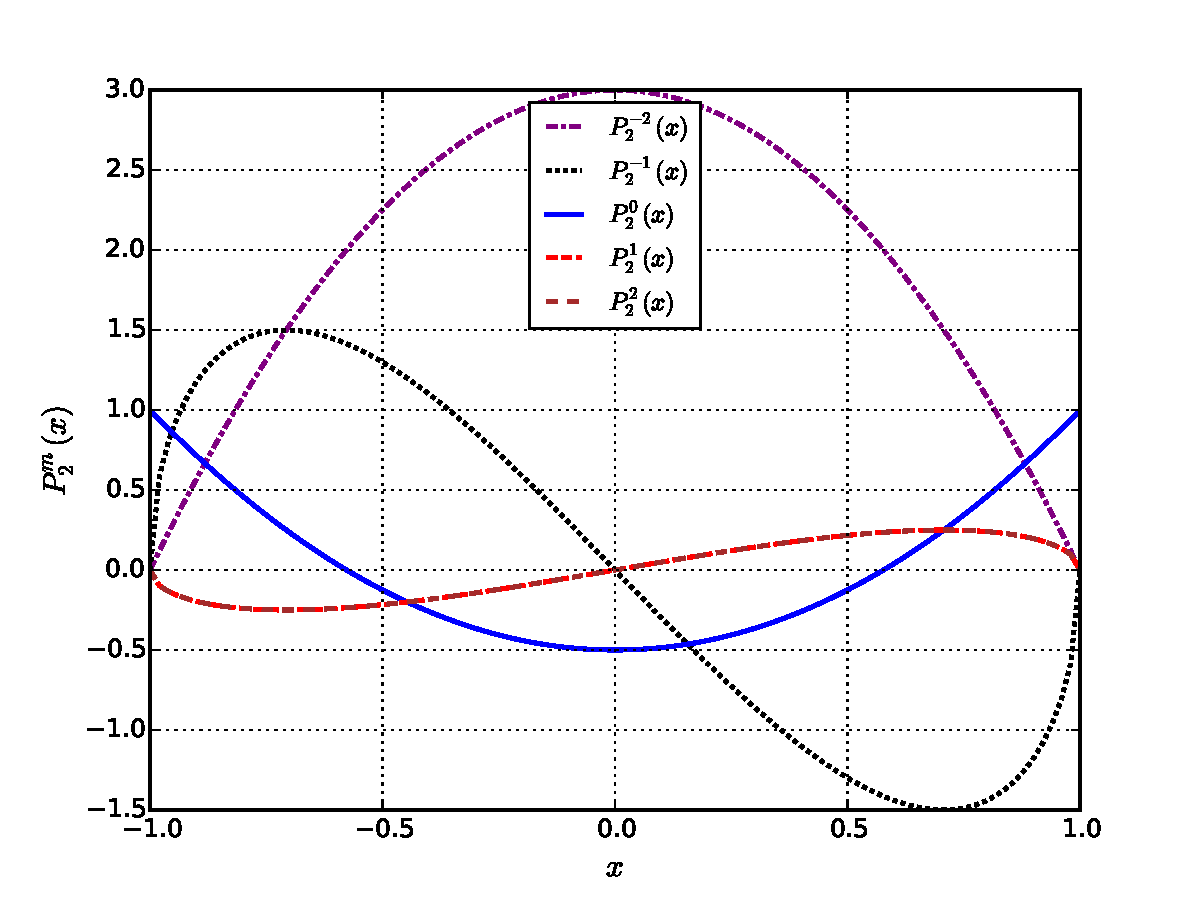
\includegraphics[angle=0,width=0.8\textwidth]{figs/fig-Legendre-Asoc-l-2.pdf}
\caption{Funciones Asociadas de Legendre: $n=2$.}
\label{fig-P2m}
\end{figure}
\begin{figure}[H]
\centering
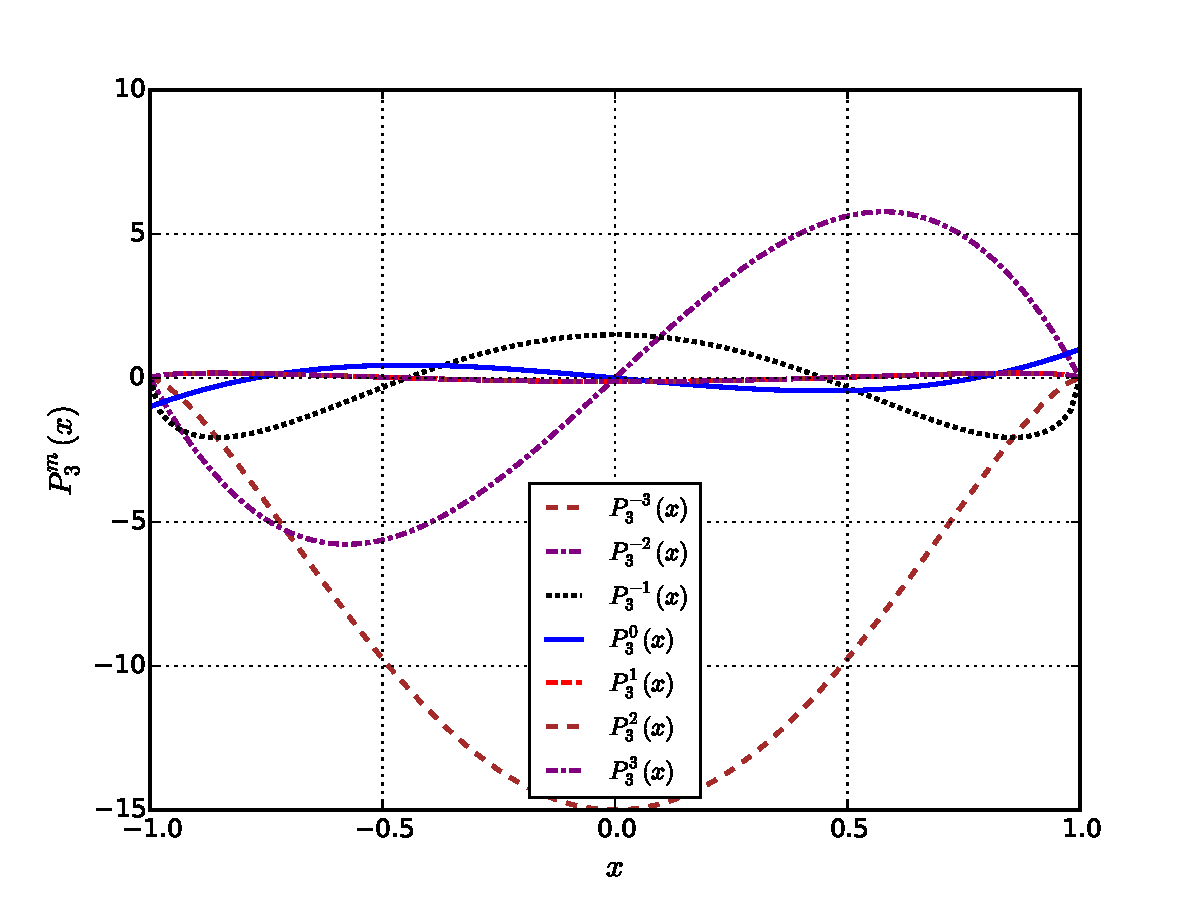
\includegraphics[angle=0,width=0.8\textwidth]{figs/fig-Legendre-Asoc-l-3.pdf}
\caption{Funciones Asociadas de Legendre: $n=3$.}
\label{fig-P3m}
\end{figure}
\subsection{F'ormula de Rodrigues}

\begin{equation}
P_{n}^{m}(x)=\frac{1}{2^{n}n!}(1-x^2)^{m/2}\frac{d^{m+n}}{dx^{m+n}}(x^2-1)^{n}.
\end{equation}

\subsection{Funci'on generadora}

\begin{equation}
\frac{(2m)! \, (1-x^2)^{m/2}}{2^{m}\, m! \, (1-2tx+t^2)^{m+1/2}} = \sum_{n=0}^{\infty} P_{n+m}^{m}(x) \, t^n
\end{equation}


\subsection{Relaciones de recurrencia}

\begin{equation}
(2n+1)xP_n^m=(n+m)P_{n-1}^m+(n+m+1)P_{n+1}^m
\end{equation}
\begin{align}
(2n+1)(1-x^2)^{1/2}P_n^m &= P_{n+1}^{m+1}-P_{n-1}^{m+1} \\
&= (n+m)(n+m-1)P_{n-1}^{m-1}-(n-m+1)(n-m+2)P_{n+1}^{m-1}
\end{align}

\subsection{Paridad}
A partir de \eqref{Pnm} y la paridad de los polinomios $P_n(x)$ encontramos que
\begin{equation}
P_n^m(-x)=(-1)^{m+m}P_n^m(x).
\end{equation}
Adem'as
\begin{equation}
P_n^m(\pm 1)=\left\{\begin{array}{cl}
(\pm 1)^n, & m=0\\
0, & m\neq 0
\end{array}\right..
\end{equation}
\subsection{Ortogonalidad}

\begin{equation}
\int_{-1}^{1}P_{n}^m(x)P_{n'}^m(x)\,dx=\frac{2}{2n+1}\frac{(n+m)!}{(n-m)!}\,\delta_{n,n'}.
\end{equation}



\section{Funciones Arm'onicas Esf'ericas}

 Volvemos ahora al problema original de encontrar las soluciones de la ecuaci'on
de Laplace. Usando (\ref{produkt1}), (\ref{Phim}) y el hecho que las funciones asociadas de Legendre son soluciones de \eqref{est22}, podemos expresar la soluci'on de \eqref{est20} como
 \begin{equation}
\Psi(r,\theta,\varphi)\propto R(r)P_l^m(\cos\theta)e^{im\varphi}.\label{est30}
 \end{equation}
Es por esto muy 'util y com'un definir las \textit{funciones arm'onicas
esf'ericas} $Y_l^m (\theta,\varphi)$ que, incorporando una normalizaci'on conveniente, son definidas por:
 \begin{eqnarray}
  Y_l^m (\theta,\varphi) := (-1)^m\sqrt\frac{2l+1}{4\pi}\cdot\sqrt\frac
   {(l-m)!}{(l+m)!}\cdot P_l^m(\cos\theta)\cdot e^{im\varphi}.\label{kugel1}
 \end{eqnarray}
  En la tabla \ref{tabelle1} se presentan los casos m'as usados.
\begin{table}[htbp]
\begin{tabular}{cc|c||cc|c}
  $l$ & $m$ & $Y_l^m $ & $l$ & $m$ & $Y_l^m $\\\hline
  0&0&$Y_0^0=\frac 1{\sqrt{4\pi}}$&2&2&$Y_2^2=\frac 14\sqrt\frac{15}{2\pi}
   \sen^2\theta e^{2i\varphi}$\\
  1&0&$Y_1^0=\sqrt\frac 3{4\pi}\cos\theta$&3&0&$Y_3^0=\sqrt\frac 7{4\pi}
  (\frac 52\cos^3\theta-\frac 32\cos\theta)$\\
  1&1&$Y_1^1=-\sqrt \frac 3{8\pi}\sen\theta e^{i\varphi}$&3&1&$Y_3^1=
  -\frac 14\sqrt\frac{21}{4\pi}\sen\theta(5\cos^2\theta-1)e^{i\varphi}$\\
  2&0&$Y_2^0=\sqrt\frac 5{4\pi}(\frac 32\cos^2\theta-\frac 12)$&3&2&$Y_3^2=
  \frac 12\sqrt\frac{105}{2\pi}\sen^2\theta\cos\theta e^{2i\varphi}$\\
  2&1&$Y_2^1=-\sqrt\frac{15}{8\pi}\sen\theta\cos\theta e^{i\varphi}$&3&3&$
  Y_3^3=-\frac 14\sqrt\frac{35}{4\pi}\sen^3\theta e^{3i\varphi}$
 \end{tabular}
\caption{Algunas funciones arm'onicas esf'ericas com'unmente usadas
($l,m=0,\ldots,3$).}
\label{tabelle1}
\end{table}

Como consecuencia de su definici'on, las funciones arm'onicas esf'ericas satisfacen las siguientes 'utiles
propiedades:
 \begin{itemize}
  \item \textit{Simetr'ia}:
   \begin{eqnarray}
    Y_l^{-m} = (-1)^m (Y_l^m)^*.\label{kugel2}
   \end{eqnarray}
  \item \textit{Ortonormalidad}:
  \begin{equation}
  \oint Y_l^m (\theta,\varphi)\cdot (Y_{l'}^{m'})^*(\theta,\varphi)\, d\Omega
=\int_0^{2\pi}\int_0^\pi Y_l^m (\theta,\varphi)  \cdot
(Y_{l'}^{m'})^*(\theta,\varphi)\, \sen\theta d\theta d\varphi   =
\delta_{ll'}\delta_{mm'},
\label{est33}
\end{equation}
 donde $d\Omega = \sen\theta d\theta d\varphi$ es el elemento de 'angulo
s'olido.

\item Como consecuencia de la ortogonalidad de las funciones $Y_l^m$, 'estas son linealmente independientes.

 \item Las funciones $Y_l^m $ forman un sistema completo de funciones. Toda
funci'on $f(\theta,\varphi)$ que satisface
\begin{equation}
    \int |f(\theta,\varphi)|^2 d\Omega <\infty,
\end{equation}
pueden ser desarrollada en t'erminos de funciones arm'onicas esf'ericas:
\begin{eqnarray}
f(\theta,\varphi) = \sum_{l=0}^\infty\sum_{m=-l}^l a_{lm}Y_l^m (\theta,\varphi),
\end{eqnarray}
con coeficientes $a_{lm}$ dados por
\begin{equation}
a_{lm}=\oint f(\theta,\varphi)(Y_{l}^{m})^*(\theta,\varphi)\,d\Omega.
\end{equation}

\item La completitud de $Y_l^m $ se expresa por:
\begin{equation}
    \sum_{l=0}^\infty\sum_{m=-l}^l (Y_l^m)^*(\theta,\varphi)
    Y_l^m (\theta',\varphi') = \delta(\varphi-\varphi')\delta(\cos\theta-
    \cos\theta').
\end{equation}
\item Las  funciones arm'onicas esf'ericas satisfacen
 \begin{eqnarray}
  \hat{L}^2(\theta,\varphi) Y_l^m  = l(l+1)Y_l^m ,
 \end{eqnarray}
donde $\hat{L}^2$ es el operador definido por
 \begin{eqnarray}
  -\hat{L}^2 :=
\frac{1}{\sen\theta}\frac{\partial}{\partial\theta}\left(\sen\theta\frac{
\partial}{\partial
  \theta}\right)+\frac 1{\sen^2\theta}\frac{\partial^2}{\partial \varphi^2}.
 \end{eqnarray}
 En otras palabras, las funciones $Y_l^m $ son funciones propias del operador
$\hat{L}^2$, con valor propio $l(l+1)$. En t'erminos de $\hat{L}^2$, podemos
escribir el operador de Laplace como:
 \begin{equation}
  \nabla^2 = \frac 1r\frac{\partial^2}{\partial r^2}\left( r \cdot\right) -
\frac{1}{r^2}\hat{L}^2.
\end{equation}
 \end{itemize}

\begin{figure}[H]
\centering
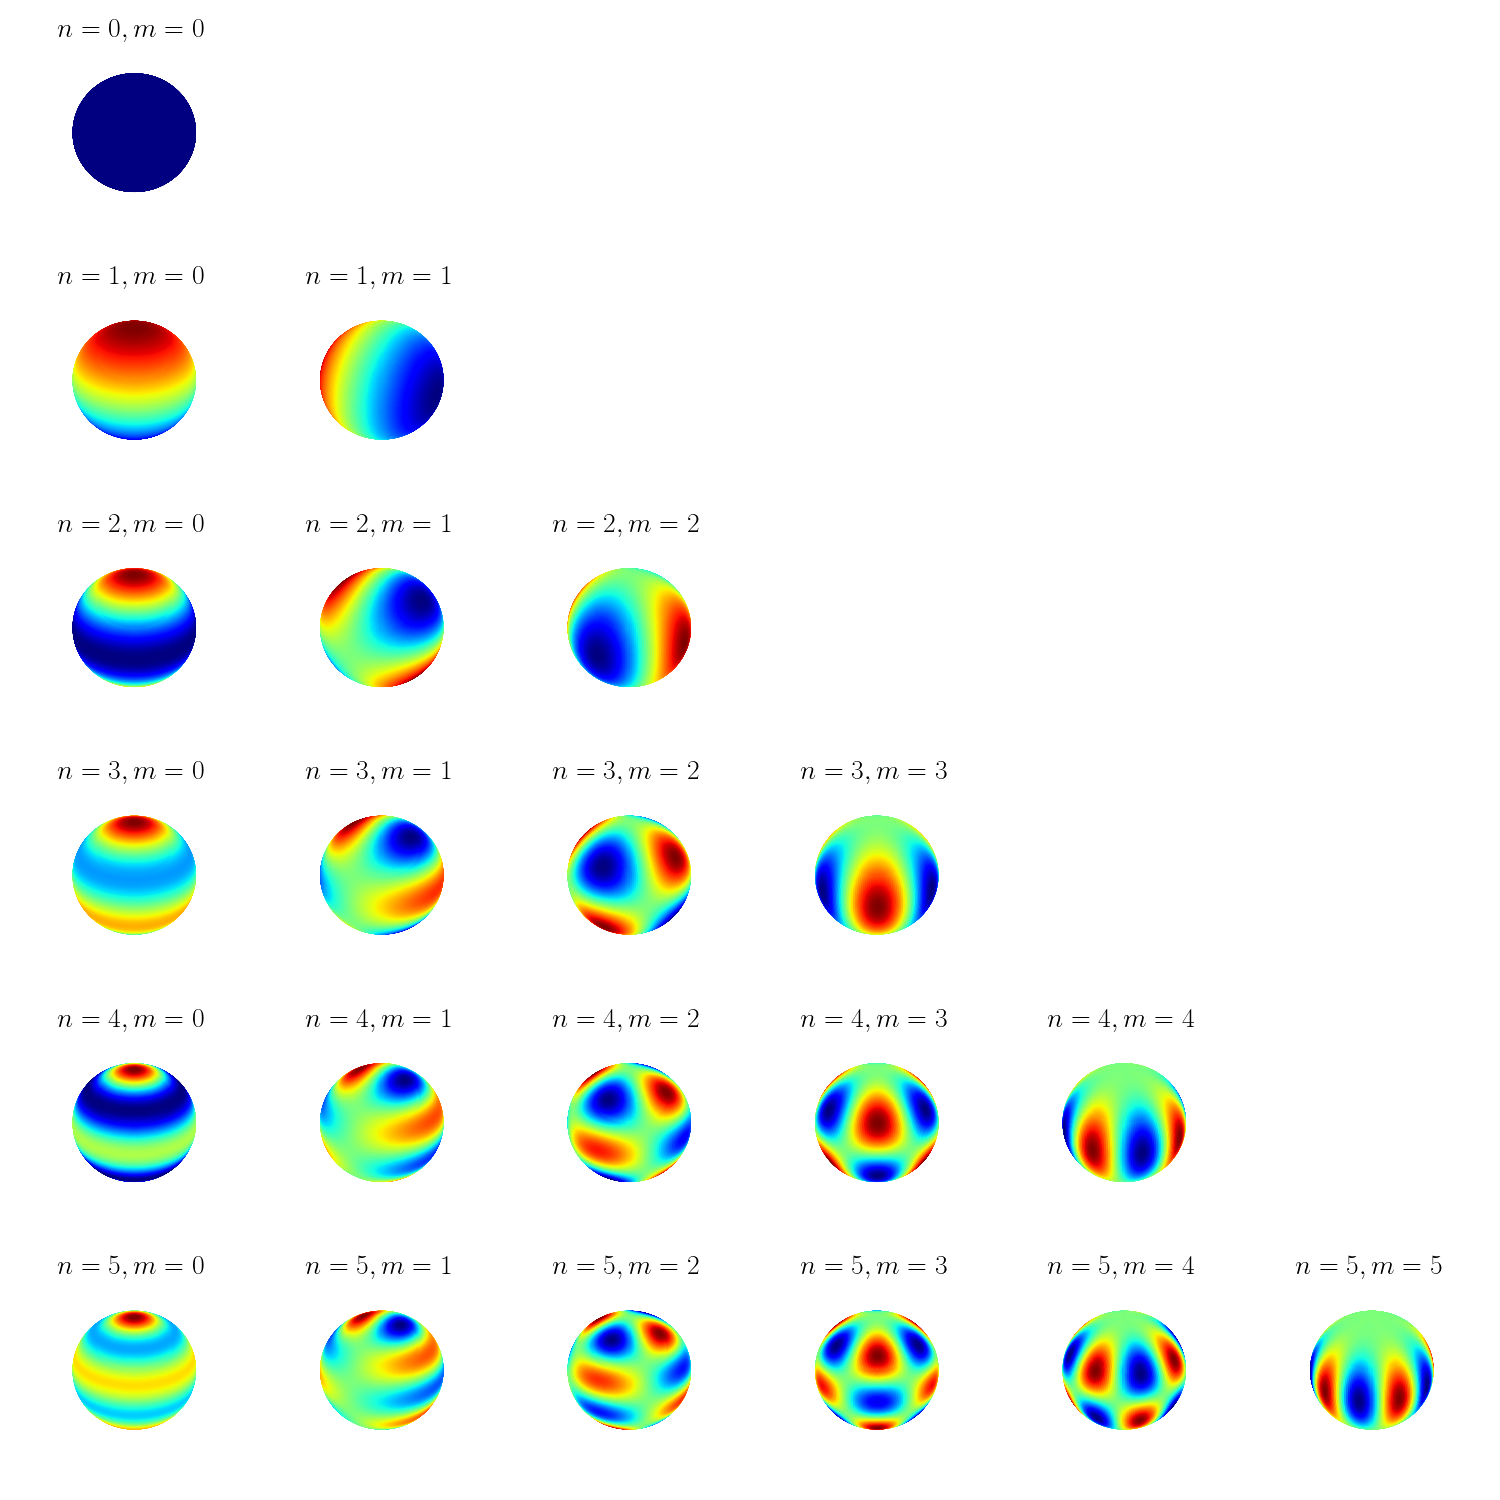
\includegraphics[angle=0,width=0.95\textwidth]{figs/fig-Aes3Dcolores.png}
\caption{Representaci'on gr'afica de (la parte real de) algunas funciones arm'onicas esf'ericas. C'odigo Python \href{https://github.com/gfrubi/FM2/blob/master/figuras-editables/Graficos-AE-esfera-colores.py}{aqu\'i}.}
\label{fig-Aes}
\end{figure}

\subsubsection{Teorema de adici'on de arm'onicos esf'ericos}
\begin{equation}
P_n(\cos\gamma) = \frac{4\pi}{2n+1} \sum_{m=-n}^n Y_n^m(\theta_1,\varphi_1)(Y_n^{m})^\ast(\theta_2,\varphi_2),
\end{equation}
donde $\gamma$ es el el 'angulo entre las direcciones definidas por los pares $(\theta_1,\varphi_1)$ y $(\theta_2,\varphi_2)$, por lo que est'an relacionados por
\begin{equation}
\cos\gamma = \cos\theta_1\cos\theta_2 + \sin\theta_1\sin\theta_2\cos(\varphi_1-\varphi_1).
\end{equation}

Un caso particular interesante de esta identidad se encuentra cuando ambas direcciones son iguales, de modo que  $\theta_1=\theta_2=\theta$ y $\varphi_1=\varphi_2=\varphi$, de modo que $\gamma=0$ y entonces
\begin{equation}
P_n(0) = \frac{4\pi}{2n+1} \sum_{m=-n}^n \left|Y_n^m(\theta,\varphi)\right|^2.
\end{equation}
De aqu'i obtenos directamente que
\begin{equation}
\sum_{m=-n}^n \left|Y_n^m(\theta,\varphi)\right|^2 = \frac{2n+1}{4\pi},
\end{equation}
lo que adem'as permite encontrar la siguiente cota superior para el m'odulo de las funciones arm'onicas esf'ericas:
\begin{equation}
\left|Y_n^m(\theta,\varphi)\right| \le \sqrt{\frac{2n+1}{4\pi}}.
\end{equation}

El teorema de adici'on es muy 'util en F'isica puesto que permite realizar expansiones de funciones como $\left|\vec{x}_1-\vec{x}_2\right|^{-1}$ que aparece com'unmente en distintas expresiones

Si $r_2<r_1$, con $r_1=\left|\vec{x}_1\right|$ y $r_2=\left|\vec{x}_2\right|$ entonces
\begin{equation}
\frac{1}{\left|\vec{x}_1-\vec{x}_2\right|} = \frac{1}{\sqrt{r_1^2+r_2^2-2r_1r_2\cos\gamma}} = \frac{1}{r_1}\frac{1}{\sqrt{1+t^2-2t\cos\gamma}},
\end{equation}
donde hemos definido $t:=r_2/r_1 <1$. Entonces
\begin{align}
\frac{1}{\left|\vec{x}_1-\vec{x}_2\right|} &= \frac{1}{r_1}\sum_{n=0}^\infty P_n(\cos\gamma)ṭ^n \\
&= \frac{1}{r_1}\sum_{n=0}^\infty t^n\frac{4\pi}{2n+1} \sum_{m=-n}^n Y_n^m(\theta_1,\varphi_1)(Y_n^{m})^\ast(\theta_2,\varphi_2)  \\
&= 4\pi \sum_{n,m}\frac{1}{2n+1}\frac{r_2^n}{r_1^{n+1}} Y_n^m(\theta_1,\varphi_1)(Y_n^{m})^\ast(\theta_2,\varphi_2).
\end{align}
En com'un encontrar esta identidad escrita de la siguiente forma:
\begin{align}
\frac{1}{\left|\vec{x}-\vec{x}'\right|} 
&= 4\pi \sum_{n,m}\frac{1}{2n+1}\frac{r_<^n}{r_>^{n+1}}Y_n^m(\theta,\varphi)(Y_n^{m})^\ast(\theta',\varphi'),
\end{align}
donde $r_> = max(r,r')$ y $r_< = min(r,r')$.

\subsubsection{Ecuaci'on de Laplace y arm'onicos esf'ericos}
En el caso de la ecuaci'on de Laplace, podemos entonces usar el resultado en \eqref{loes2}, con $Q=n(n+1)$, para escribir una expresi'on general para la soluci'on (finita para $\theta=0$ y $\theta=\pi$), en coordenadas esf'ericas:
\begin{equation}
\Psi(r,\theta,\varphi)=\sum_{n=0}^\infty\sum_{m=-n}^n\left(A_{nm}r^n+\frac{B_{nm}}{r^{n+1}}\right)Y_n^m(\theta,\varphi).
\end{equation}
\chapter{Funciones de Bessel}
\section{Ecuaci'on de Bessel}
Consideraremos aqu'i la ecuaci'on diferencial de Bessel con argumento complejo, $z\in\mathbb{C}$, ya que sus soluciones suminitrar'an funciones que satisfacen la E.D.O. de Bessel con variables reales y la E.D.O. modificada de Bessel. Finalmente, buscaremos soluciones de la ecuaci'on con un coeficiente $\nu^ 2$ real y positivo, pero no necesariamente entero.

En resumen, buscamos soluciones de la ecuaci'on
\begin{equation}\label{Besselec1}
z\frac{d\ }{dz}\left(z\frac{dy}{dz}\right)+(z^2-\nu^2)y(z)=0,
\end{equation}
que puede ser escrita como
\begin{equation}\label{EDOBessel}
y'' + \frac{1}{z} y' + \left( 1 - \frac{\nu^2}{z^2} \right)y = 0.
\end{equation}


\section{Soluci'on en serie en torno a $z = 0$}\label{secsolBess}
Buscaremos soluciones en serie de potencias de \eqref{Besselec1}. Es conveniente encontrar una serie en torno a $z=0$ (el ``punto m'as sim'etrico de la ecuaci'on''). Sin embargo, este punto es un punto singular de la ecuaci'on, por lo que en general no es posible expresar la soluci'on como una serie de la forma $y(z) = \sum_{n=0}^\infty a_n z^n$. Para entender esto m'as claramente, recuerde que los coeficientes $a_n$ ser'ian entonces proporcionales a la $n-$'esima derivada de la soluci'on $y(z)$, evaluada en $z=0$. Por lo tanto, encontrar la soluci'on de esta forma es equivalente a requerir que cada una de las derivadas de la soluci'on sean finitas en $z=0$. Como la E.D.O. es de segundo orden, se requieren dos condiciones iniciales, que pueden elegirse como $y(0)$ e $y'(0)$. Las derivadas superiores quedan determinadas por la E.D.O. Sin embargo, vemos de 
\eqref{EDOBessel} que $y''(0)$ (y las derivadas superiores) ser'a en general divergente, a'un en el caso en que se elija $y'(0)$, debido al t'ermino $({\nu^2}/{z^2})y(z)$. 

Afortunadamente, s'i es posible encontrar soluciones de la forma\footnote{Una forma alternativa de verificar que este es el caso es realizar el cambio de variable $y(z):=z^\alpha f(z)$ y ajustar la constante $\alpha$ de modo que la E.D.O. resultante para la funci'on $f(z)$ s'i pueda expresarse como una serie de potencias de la forma $f(z) = \sum_{n=0}^\infty a_n z^n$.}
\begin{equation}\label{yzasum}
y(z) = z^\alpha \sum_{n=0}^\infty a_n z^n = \sum_{n=0}^\infty a_n z^{n+\alpha},
\end{equation}
donde $\alpha$ es una constante (no necesariamente un entero) que ser'a elegida convenientemente. Suponiendo \eqref{yzasum}, las derivadas de $y(z)$ adoptan la forma siguiente:
\begin{equation}
y' = \sum_{n=0}^\infty (n+\alpha) a_n z^{n+\alpha-1}, \quad
y'' = \sum_{n=0}^\infty (n+\alpha)(n+\alpha-1) a_n z^{n+\alpha-2}.
\end{equation}

Substituyendo estas expansiones en \eqref{EDOBessel} encontramos
\begin{align}
0 &=  z^2 y'' + z y' + \left( z^2 - \nu^2 \right) y  \\
  &= \sum_{n=0}^\infty (n+\alpha)(n +\alpha - 1)\, a_n z^{n+\alpha}
  + \sum_{n=0}^\infty (n+\alpha)\, a_n z^{n+\alpha} + \sum_{n=0}^\infty a_n z^{n+\alpha+2}
  - \nu^2\sum_{n=0}^\infty a_n z^{n+\alpha}  \\
 &=  \sum_{n=0}^\infty \left[ (n+\alpha)^2 -\nu^2 \right] a_n z^{n+\alpha}
  + \sum_{n=2}^\infty a_{n-2} z^{n+\alpha} \\
 &= (\alpha^2-\nu^2)a_0\,z^\alpha+\left[ (\alpha+1)^2 -\nu^2 \right] a_1\,z^{\alpha+1}
 + \sum_{n=2}^\infty \left[ \left( (n+\alpha)^2 -\nu^2 \right) a_n+a_{n-2}\right]  z^{n+\alpha}.
\end{align}
Por lo tanto, los coeficientes deben satisfacer las siguientes condiciones:
\begin{equation}\label{rrBess}
(\alpha^2-\nu^2)a_0=0,  \qquad \left[ (\alpha+1)^2 -\nu^2 \right] a_1=0, \qquad 
\left( (n+\alpha)^2 -\nu^2 \right) a_n+a_{n-2}=0.
\end{equation}
Encontramos as'i una relaci'on de recurrencia entre $a_n$ y $a_{n-2}$, que permite entonces expresar todos los coeficientes $a_n$ con $n$ par en t'erminos de $a_0$ y todos los con $n$ impar en t'erminos de $a_1$. 

Como buscamos soluciones no nulas, suponemos primero que $a_0\neq 0$. Entonces la primera condici'on en \eqref{rrBess} implica que $\alpha=\pm\nu$. En este caso la segunda condici'on en \eqref{rrBess} se reduce a $(1+2\alpha)a_1=0$. Analizaremos primero el caso gen'erico en que $\alpha\neq -1/2$. Entonces necesariamente $a_1=0$ y s'olo los coeficientes pares, de la forma $a_{2k}$, $k=0,1,2,\cdots$, ser'an no nulos. De la relaci'on de recurrencia en \eqref{rrBess} obtenemos
\begin{equation}\label{anan-2}
a_n=-\frac{a_{n-2}}{n(n+2\alpha)}.
\end{equation}
Aplicaci'on sucesiva de \eqref{anan-2} conduce a
\begin{align}
a_{2 k} &= \frac{a_0(-1)^k}{2^{2k}k!}\frac{1}{(1+\alpha)(2+\alpha)(3+\alpha)\cdots (k+\alpha)}\\
&= \frac{a_0 (-1)^k}{2^{2k} k!}\frac{\Gamma(1+\alpha)}{\Gamma(k +\alpha+ 1) }, \qquad k=0,1,2,\cdots. 
\end{align}
Aqu'i hemos introducido la funci'on Gamma, ver ap'endice \ref{app-Gamma}. Por lo tanto, para $\alpha=\nu$ hemos encontrado una soluci'on de la forma
\begin{equation}
y_\nu(z) = a_0 \sum_{k=0}^\infty \frac{(-1)^k}{2^{2k}k!}\frac{\Gamma(1+\nu)}{\Gamma(k+\nu+ 1) }
z^{2k+\nu},
\end{equation}
donde $a_0$ es una constante arbitraria. Es conveniente definir las \textit{funciones de Bessel de primera especie y orden} $\nu$, $J_\nu(z)$, como las soluciones correspondientes al caso en que $a_0:=1/2^{\nu}\Gamma(\nu+1)$, de modo que
\begin{equation}\label{Besselnu}
\boxed{J_\nu(z) = \sum_{k = 0}^\infty \frac{ (-1)^k }{ k! \Gamma(k + \nu + 1) }
\left( \frac{z}{2} \right)^{2k+\nu}.}
\end{equation}

Expandiendo los primeros t'erminos, encontramos:
\begin{align}\label{J-nu}
J_\nu(z) &= \frac{1}{\Gamma(\nu+1)}\left(\frac{z}{2}\right)^{\nu}
-\frac{1}{\Gamma(\nu+2)}\left(\frac{z}{2}\right)^{\nu+2}+ \cdots \\
&= \frac{1}{\Gamma(\nu+1)}\left(\frac{z}{2}\right)^{\nu}\left[1-\frac{1}{(\nu+1)}\left(\frac{z}{2}\right)^2+\cdots \right].
\end{align}

Como la E.D.O. de Bessel \eqref{Besselec1} depende del cuadrado de $\nu$, tendremos que 
\begin{equation}
J_{-\nu}(z) = \sum_{k = 0}^\infty \frac{ (-1)^k }{ k! \Gamma(k-\nu+1) }
\left( \frac{z}{2} \right)^{2k-\nu},
\end{equation}
es tambi'en una soluci'on (que equivale al caso $\alpha=-\nu$). 

\textit{Si $\nu$ es positivo, pero no es entero}, entonces tanto $\Gamma(k+\nu+1)$ como $\Gamma(k-\nu+1)$ asumen valores finitos y por lo tanto $J_\nu$ y $J_{-\nu}$ est'an bien definidas para todo $z$. Para valores de $z$ cercanos a cero tendremos entonces que $J_\nu\approx (z/2)^\nu/\Gamma(1+\nu)$ y $J_{-\nu}\approx (z/2)^{-\nu}/\Gamma(1-\nu)$. Por lo tanto, $J_\nu(0)=0$ mientras que  $J_{-\nu}(0)$ es divergente. Por otro lado, $J_0(0)=1$. En particular, esto muestra que $J_\nu$ y $J_{-\nu}$ \textit{son linealmente independientes si $\nu$ no es entero}.
En este caso la soluci'on general de \eqref{Besselec1} es de la forma
\begin{equation}
y(z)=c_1J_\nu(z)+c_2J_{-\nu}(z).
\end{equation}
Por razones hist'oricas y de conveniencia futura se definen adicionalmente las \textbf{funciones de Bessel de segunda especie} de orden $\nu$, $Y_\nu(z)$ (tambi'en llamadas \textbf{funciones de Neumann} y denotadas por $N_\nu(z)$), por
\begin{equation}
Y_\nu(z)=N_\nu(z):=\frac{\cos(\pi\nu)J_\nu(z)-J_{-\nu}(z)}{\sen(\pi\nu)}.
\end{equation}
Entonces la soluci'on general de \eqref{Besselec1} puede expresarse como una combinaci'on lineal de la funci'on de Bessel y de Neumann correspondiente:
\begin{equation}
y(z)=c_3J_\nu(z)+c_4Y_\nu(z).
\end{equation}


\subsubsection{Caso en que $\alpha=-1/2$}

En este caso en general tendremos que $a_0\neq 0$ y $a_1\neq 0$, y la relaci'on de recurrencia \eqref{anan-2} se reduce a 
\begin{equation}
a_n=-\frac{a_{n-2}}{n(n-1)}.
\end{equation} 
Como consecuencia encontramos que, si $n$ es par, entonces
\begin{equation}
a_{2k}=\frac{(-1)^k a_0}{(2k)!},
\end{equation}
mientras que si $n$ es impar,
\begin{equation}
a_{2k+1}=\frac{(-1)^k a_1}{(2k+1)!}.
\end{equation}

As\'i, la soluci\'on es de la forma
\begin{eqnarray}
y(z)&=&z^{-1/2}\left(\sum_{k=0}^{+\infty}a_{2k}z^{2k}+\sum_{k=0}^{+\infty}a_{2k+1}z^{2k+1} \right)\\
&=&z^{-1/2}\left(a_0\sum_{k=0}^{+\infty}\frac{(-1)^k}{(2k)!}z^{2k}+a_1\sum_{k=0}^{+\infty}\frac{(-1)^k}{(2k+1)!}z^{2k+1} \right).
\end{eqnarray}

Por lo tanto, la soluci\'on general de la E.D.O. de Bessel con $\nu^2=1/4$ es de la forma
\begin{equation}
\boxed{y(z)= z^{-1/2}\left(a_0\cos(z)+a_1\sen(z) \right).}
\end{equation}


\subsubsection{Caso en que $\alpha^2\neq\nu^2$}
Suponemos ahora que $\alpha^2\neq\nu^2$, entonces $a_0=0$ con lo cual $a_{2k}= 0$ y adem'as  $a_1\neq 0$. Luego, $(\alpha+1)^2-\nu^2=0$. Reemplazando esto \'utlimo en \eqref{rrBess}, se obtiene que
\begin{equation} \label{rrBEssimpar}
a_n=-\frac{a_{n-2}}{(n-1)(n+1+2\alpha)}.
\end{equation}
Aplicando sucesivamente \eqref{rrBEssimpar}, encontramos
\begin{eqnarray}
a_{2k+1}&=&\frac{(-1)^ka_1}{2^{2k}k!}\frac{1}{(\alpha+2)(\alpha+3)(\alpha+4)\cdots (\alpha +k+1)}\\
&=&\frac{(-1)^ka_1}{2^{2k }k!}\frac{\Gamma(\alpha+2)}{\Gamma(\alpha+k+2)}.
\end{eqnarray}

As\'i, para $\alpha=\nu-1$ se tiene que la soluci\'on toma la forma
\begin{equation}
y_\nu(z) = a_1 \sum_{k=0}^\infty \frac{(-1)^k}{2^{2k}k!}\frac{\Gamma(1+\nu)}{\Gamma(k+\nu+ 1) }
z^{2k+\nu}.
\end{equation}

Eligiendo $a_1=1/(2^{\nu}\Gamma(1+\nu))$, se obtiene nuevamente la funci\'on de Bessel de primera especie, dada por \eqref{Besselnu}.




\section{Relaciones de Recurrencia}
Las funciones de Bessel $J_\nu(z)$ satisfacen las siguientes relaciones de recurrencia:
\begin{equation}\label{rrJnu1}
J_{\nu-1}(z)+J_{\nu+1}(z)=\frac{2\nu}{z}J_\nu(z),
\end{equation}
\begin{equation}\label{rrJnu2}
J_{\nu-1}(z)-J_{\nu+1}(z)=2J'_\nu(z).
\end{equation}
Podemos verificar estas relaciones usando directamente la expresi'on en serie de potencias \eqref{Besselnu}. En efecto,
\begin{align}
J_{\nu-1}(z)+J_{\nu+1}(z) &= 
\sum_{k=0}^\infty\frac{(-1)^k}{k!\Gamma(k+\nu)}\left(\frac{z}{2}\right)^{2k+\nu-1} 
+\sum_{k=0}^\infty\frac{(-1)^k}{k!\Gamma(k+\nu+2)}\left(\frac{z}{2}\right)^{2k+\nu+1} \label{idJ1}\\
&= \frac{2}{z}\left[\sum_{k=0}^\infty\frac{(-1)^k}{k!\Gamma(k+\nu)}\left(\frac{z}{2}\right)^{2k+\nu} 
+\sum_{k=0}^\infty\frac{(-1)^k}{k!\Gamma(k+\nu+2)}\left(\frac{z}{2}\right)^{2k+\nu+2}\right] \\
&= \frac{2}{z}\left[\sum_{k=0}^\infty\frac{(-1)^k(k+\nu)}{k!\Gamma(k+\nu+1)}\left(\frac{z}{2}\right)^{2k+\nu} \right. \nonumber\\
&\ \left.\qquad\qquad +\sum_{k=1}^\infty\frac{(-1)^{k-1}}{(k-1)!\Gamma(k+\nu+1)}\left(\frac{z}{2}\right)^{2k+\nu}\right] \\
&= \frac{2}{z}\left[\sum_{k=0}^\infty\frac{(-1)^k(k+\nu)}{k!\Gamma(k+\nu+1)}\left(\frac{z}{2}\right)^{2k+\nu}  +\sum_{k=1}^\infty\frac{(-1)^{k-1}}{\Gamma(k+\nu+1)}\frac{k}{k!}\left(\frac{z}{2}\right)^{2k+\nu}\right] \\
&= \frac{2}{z}\sum_{k=0}^\infty\frac{(-1)^k}{k!\Gamma(k+\nu+1)}\left[(k+\nu)-k\right]\left(\frac{z}{2}\right)^{2k+\nu} \label{idJ2}\\
&= \frac{2\nu}{x}\sum_{k=0}^\infty\frac{(-1)^k}{k!\Gamma(k+\nu+1)}\left(\frac{z}{2}\right)^{2k+\nu} \\
&= \frac{2\nu}{z}J_\nu(z).
\end{align}
De manera an'aloga, realizando ahora la resta de $J_{\nu-1}(z)$ y $J_{\nu+1}(z)$ obtenemos (ver \eqref{idJ1} y \eqref{idJ2}):
\begin{align}
J_{\nu-1}(z)-J_{\nu+1}(z) &= 
\sum_{k=0}^\infty\frac{(-1)^k}{k!\Gamma(k+\nu)}\left(\frac{z}{2}\right)^{2k+\nu-1} 
-\sum_{k=0}^\infty\frac{(-1)^k}{k!\Gamma(k+\nu+2)}\left(\frac{z}{2}\right)^{2k+\nu+1} \\
&= \frac{2}{z}\sum_{k=0}^\infty\frac{(-1)^k}{k!\Gamma(k+\nu+1)}\left[(k+\nu)+k\right]\left(\frac{z}{2}\right)^{2k+\nu}\\
&= \sum_{k=0}^\infty\frac{(-1)^k}{k\Gamma(k+\nu+1)}(2k+\nu)\left(\frac{z}{2}\right)^{2k+\nu-1}\\
&= \frac{d\ }{dz}\sum_{k=0}^\infty\frac{(-1)^k}{k!\Gamma(k+\nu+1)}\left(\frac{z}{2}\right)^{2k+\nu} \\
&= J'_\nu(z).
\end{align}
A partir de las relaciones \eqref{rrJnu1} y \eqref{rrJnu2} podemos derivar otras relaciones. Por ejemplo, sumando \eqref{rrJnu1} y \eqref{rrJnu2} llegamos a
\begin{align}
J_{\nu-1}(z) &= J'_{\nu}(z)+\frac{\nu}{z}J_\nu(z) \label{Jnu-1JpJ}\\
&= z^{-\nu}\frac{d\ }{dz}\left[z^\nu J_\nu(z)\right]. \label{Jnu-1JpJ2}
\end{align}
Similarmente, la suma de \eqref{rrJnu1} y \eqref{rrJnu2} conduce a 
\begin{align}
J_{\nu+1}(z) &= -J'_{\nu}(z)+\frac{\nu}{z}J_\nu(z) \label{rrJni+1} \\
&= -z^{\nu}\frac{d\ }{dz}\left[z^{-\nu} J_\nu(z)\right]. \label{rrJni+2}
\end{align}
Finalmente, podemos verificar que estas relaciones implican que las funciones $J_\nu(z)$ satisfacen la ecuaci'on de Bessel. A partir de \eqref{Jnu-1JpJ} tenemos que $zJ'_\nu=zJ_{\nu-1}-\nu J_\nu$. Derivando y multiplicando por $z$ esta relaci'on, tenemos que
\begin{align}
z\frac{d\ }{dz}(zJ'_\nu) &= z\left(J_{\nu-1}+zJ'_{\nu-1}-\nu J'_\nu\right)\\
&= zJ_{\nu-1}+z^2J'_{\nu-1}-\nu zJ'_\nu. \label{zdzJ'}
\end{align}
Usando \eqref{rrJni+1} (reemplazando $\nu$ por $\nu-1$) para reescribir el segundo t'ermino de \eqref{zdzJ'} y nuevamente \eqref{Jnu-1JpJ} en el 'ultimo t'ermino, llegamos a
\begin{align}
z\frac{d\ }{dz}(zJ'_\nu) &= zJ_{\nu-1}+z\left[(\nu-1)J_{\nu-1}-zJ_\nu\right]-\nu (zJ_{\nu-1}-\nu J_\nu) \\
&= -(z^2-\nu^2) J_\nu,
\end{align}
que es equivalente a la ecuaci'on \eqref{Besselec1}.

\subsection{Representaci'on integral ***}
Las funciones de Bessel de orden $\nu$ y argumento real pueden expresarse como la siguiente integral en el plano complejo
\begin{equation}\label{RIJnu}
\boxed{J_\nu(x)=2\pi i\int_{\cal C}e^{(x/2)(t-t^{-1})}t^{-\nu-1}dt,}
\end{equation}
donde $t\in\mathbb{C}$ est'a integrado sobre el contorno $\cal C$ indicado en la figura XXX.

Podemos probar esta relaci'on a partir de la siguiente representaci'on de la funci'on Gamma (ver, por ejemplo, la expresi'on (11.21) \cite{Hassani}):
\begin{equation}\label{1sGint}
\frac{1}{\Gamma(z)}=\frac{1}{2\pi i}\int_{\cal C}e^t t^{-z}dt.
\end{equation}

Primero, reescribimos el integrando de \eqref{RIJnu} como
\begin{align}
e^{(x/2)(t-t^{-1})}t^{-\nu-1} &= e^{xt/2}e^{-x/2t}t^{-\nu-1} \\
&= e^{xt/2}\left[\sum_{k=0}^\infty\frac{1}{k!}\left(\frac{-x}{2t}\right)^k\right]t^{-\nu-1} \\
&= \sum_{k=0}^\infty\frac{(-1)^k}{k!}\left(\frac{x}{2}\right)^ke^{xt/2}t^{-k-\nu-1}. \label{exttsum}
\end{align}
Entonces, integrando esta relaci'on sobre $\cal C$, encontramos
\begin{align}
\int_{\cal C}e^{(x/2)(t-t^{-1})}t^{-\nu-1}dt &= \sum_{k=0}^\infty\frac{(-1)^k}{k!}\left(\frac{x}{2}\right)^k\int_{\cal C}e^{xt/2}t^{-k-\nu-1}dt .
\end{align}
Finalmente, realizando el cambio de variable $x':=xt/2$ y usando \eqref{1sGint} reescribimos al 'ultima integral como
\begin{align}
\int_{\cal C}e^{xt/2}t^{-k-\nu-1}dt &= \frac{2}{x}\int_{\cal C}e^{t'}\left(\frac{2t'}{x}\right)^{-k-\nu-1}dt' \\
&= \left(\frac{2}{x}\right)^{-k-\nu}\int_{\cal C}e^{t'}t'^{-k-\nu-1}dt' \\
&= \left(\frac{2}{x}\right)^{-k-\nu}\frac{2\pi i}{\Gamma(k+\nu+1)}. \label{intCG2}
\end{align}
Sustituyendo \eqref{intCG2} en \eqref{exttsum} llegamos directamente al resultado deseado, luego de indentificar la expansi'on en serie de potencias \eqref{Besselnu} de la funci'on $J_\nu(x)$.

A partir de \eqref{RIJnu} podemos encotrar la expresi'on alternativa:
\begin{equation}
\boxed{J_\nu(x)=\frac{1}{\pi}\int_0^\pi\cos(\nu\theta-x\sen\theta)d\theta-\frac{\sen(\nu\pi)}{\pi}\int_0^\infty e^{-\nu t-x\senh t}dt.}
\end{equation}

\subsection{Forma asint'otica}
A partir de la representaci'on integral \eqref{RIJnu} es posible encontrar una expresi'on asint'otica para las funciones de Bessel, v'alida para valores ``grandes'' de $x$:
\begin{equation}\label{asinJnu}
J_\nu(x)\approx \sqrt{\frac{2}{\pi x}}\cos\left(x-\frac{\nu\pi}{2}-\frac{\pi}{4}\right), 
\qquad x\gg\left|\nu^2-\frac{1}{4}\right|.
\end{equation}

\subsection{Ceros de las funciones de Bessel}
Frecuentemente, es necesario evaluar las raices, o ceros, de las funciones de Bessel. La funci'on de Bessel $J_\nu(x)$ tiene infinitas raices (ver, por ejemplo, figura \ref{fig-Jn}). Denotaremos $\alpha_{\nu,n}$ a la $n$-'esima raiz de la funci'on $J_\nu(x)$, es decir, tal que $J_\nu(\alpha_{\nu,n})=0$ y $\alpha_{\nu,n+1}<\alpha_{\nu,n}$, $n=1,2,\cdots$. Los valores de estas raices son calculadas num'ericamente a partir, por ejemplo, de la expresi'on en serie \eqref{Besselnu} para las funciones de Bessel. En la tabla \ref{tabla:alphanun} se muestran algunos de estos ceros.:
\begin{table}
\begin{center}
\begin{tabular}{ccccccc}
\hline $\alpha_{m,n}$ & $n=1$ & $n=2$ & $n=3$ & $n=4$ & $n=5$ \\ \hline 
$m=0$ & 2.4048255 &  5.5200781 &  8.6537279 & 11.7915344 & 14.9309177\\
$m=1$ & 3.8317059 &  7.0155866 & 10.1734681 & 13.3236919 & 16.4706300\\
$m=2$ & 5.1356223 &  8.4172441 & 11.6198411 & 14.7959517 & 17.9598194 \\
$m=3$ & 6.3801619 &  9.7610231 & 13.0152007 & 16.2234661 & 19.4094152 \\
$m=4$ & 7.5883424 & 11.0647094 & 14.3725366 & 17.6159660 & 20.8269329 \\
\hline 
\end{tabular} 
\caption{Las primeras ra'ices $\alpha_{m,n}$ de $J_m(x)$, $m=0,1,2,3,4$. C'odigo Python disponible en \href{https://github.com/gfrubi/FM2/blob/master/Notebooks/Bessel-Ceros.ipynb}{este} notebook.}
\label{tabla:alphanun}
\end{center}
\end{table}
\begin{figure}[H]
\centering
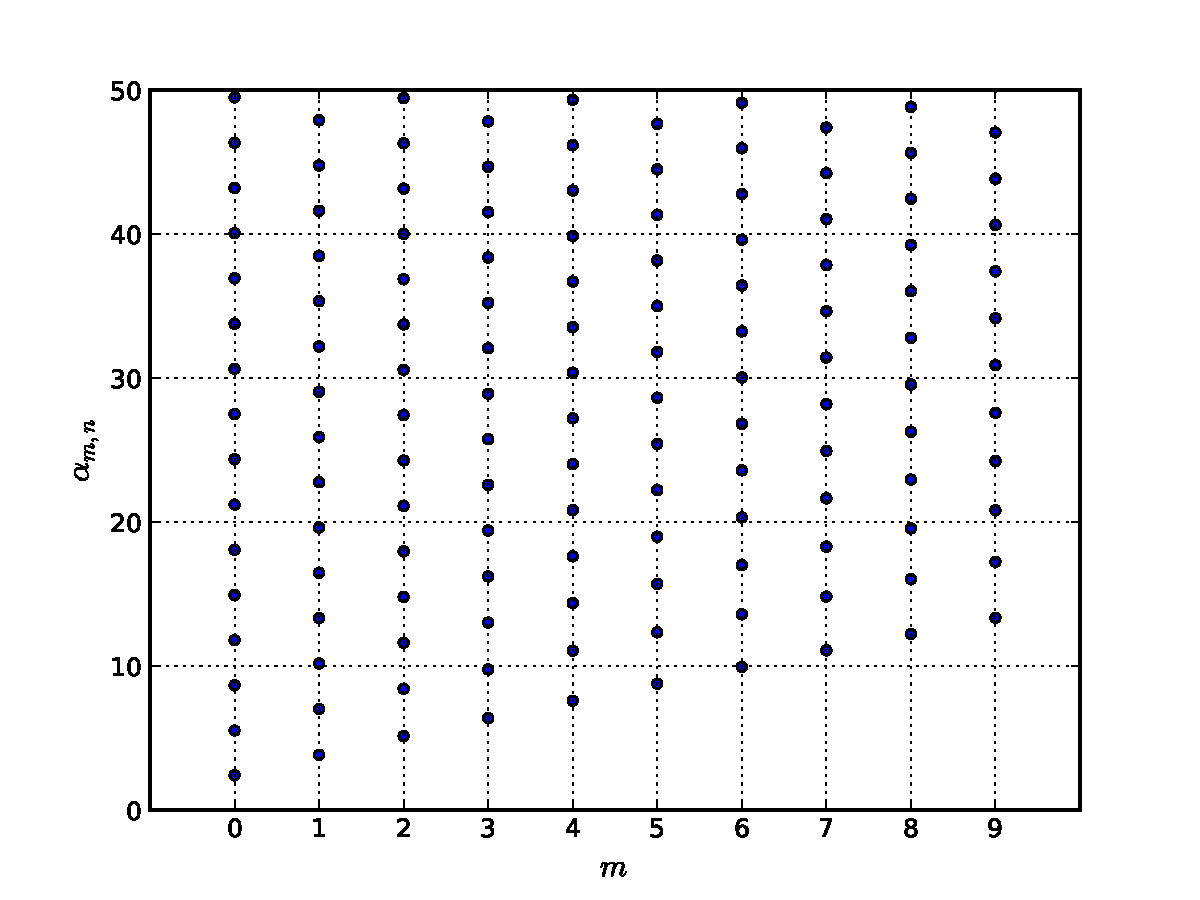
\includegraphics[angle=0,width=0.7\textwidth]{figs/fig-Bessel-ceros-01.pdf}
\caption{Algunos ceros de las funciones $J_m(x)$. C'odigo Python disponible en \href{https://github.com/gfrubi/FM2/blob/master/Notebooks/Bessel-Ceros.ipynb}{este} notebook.}
\label{fig-0Jn}
\end{figure}
\begin{figure}[H]
\centering
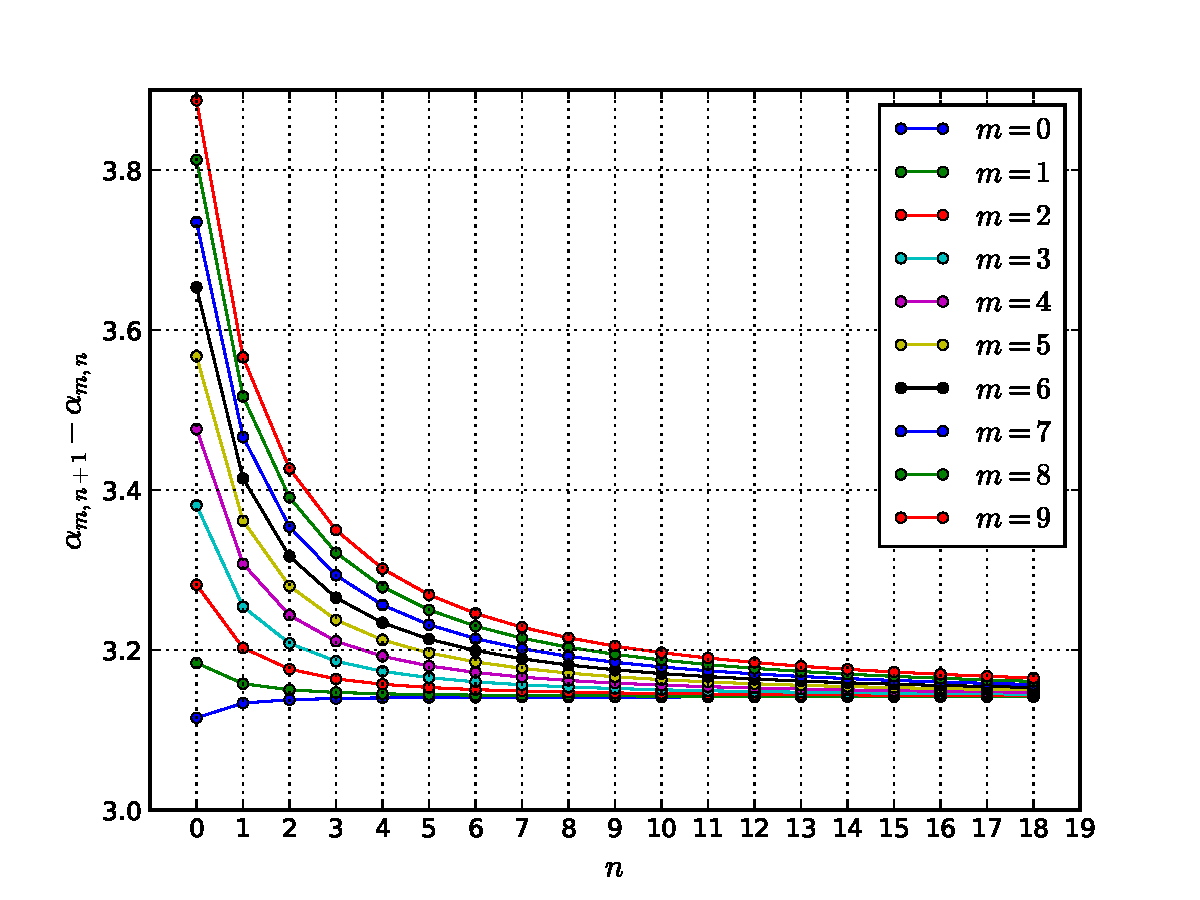
\includegraphics[angle=0,width=0.7\textwidth]{figs/fig-Bessel-ceros-02.pdf}
\caption{Diferencias entre ceros sucesivos de las funciones $J_m(x)$. C'odigo Python disponible en \href{https://github.com/gfrubi/FM2/blob/master/Notebooks/Bessel-Ceros.ipynb}{este} notebook.}
\label{fig-0Jn2}
\end{figure}
Es tambi'en frecuente requerir calcular las \textit{raices de las derivadas de las funciones de Bessel}. 'Estas ser'an denotadas por $\beta_{\nu,n}$ y entonces satisfacen $J'_\nu(\beta_{\nu,n})=0$ y $\beta_{\nu,n+1}<\alpha_{\beta,n}$, $n=1,2,\cdots$. La tabla  \ref{tabla:betanun} resume algunos de estos valores:
\begin{table}
\begin{center}
\begin{tabular}{ccccccc}
\hline $\beta_{m,n}$ & $n=1$ & $n=2$ & $n=3$ & $n=4$ & $n=5$ \\ \hline 
$m=0$ & 3.8317059 &  7.0155866 & 10.1734681 & 13.3236919 & 16.4706300\\
$m=1$ & 1.8411837 &  5.3314427 &  8.5363163 & 11.7060049 & 14.8635886 \\
$m=2$ & 3.0542369 &  6.7061331 &  9.9694678 & 13.1703708 & 16.3475223 \\
$m=3$ & 4.2011889 &  8.0152366 & 11.3459243 & 14.5858482 & 17.7887478 \\
$m=4$ & 5.3175531 &  9.2823962 & 12.6819084 & 15.9641070 & 19.1960288 \\
\hline 
\end{tabular} 
\caption{Las primeras ra'ices $\beta_{m,n}$ de $J'_m(x)$, $m=0,1,2,3,4$. C'odigo disponible en \href{https://github.com/gfrubi/FM2/blob/master/Notebooks/Bessel-Ceros.ipynb}{este} notebook.}
\label{tabla:betanun}
\end{center}
\end{table}

\subsection{Relaciones de Ortogonalidad}
Para $\nu\ge 0$, $\quad n,m=1,2,\cdots$ y $a>0$, tenemos que
\begin{equation}\label{roJnualpha}
\int_0^a J_\nu\left(\frac{\alpha_{\nu,n}}{a}\rho\right)J_\nu\left(\frac{\alpha_{\nu,m}}{a}\rho\right)\rho \, d\rho=\delta_{n,m}\frac{a^2}{2}\left[J_{\nu+1}(\alpha_{\nu,n})\right]^2.
\end{equation}
Similarmente,
\begin{equation}\label{roJnubeta}
\int_0^a J_\nu\left(\frac{\beta_{\nu,n}}{a}\rho\right)J_\nu\left(\frac{\beta_{\nu,m}}{a}\rho\right)\rho \, d\rho=\delta_{n,m}\frac{a^2}{2}\left(1-\frac{\nu^2}{\beta_{\nu,n}^2}\right)\left[J_\nu(\beta_{\nu,n})\right]^2.
\end{equation}

\section{Funciones de Bessel de orden entero}
\begin{figure}[H]
\centering
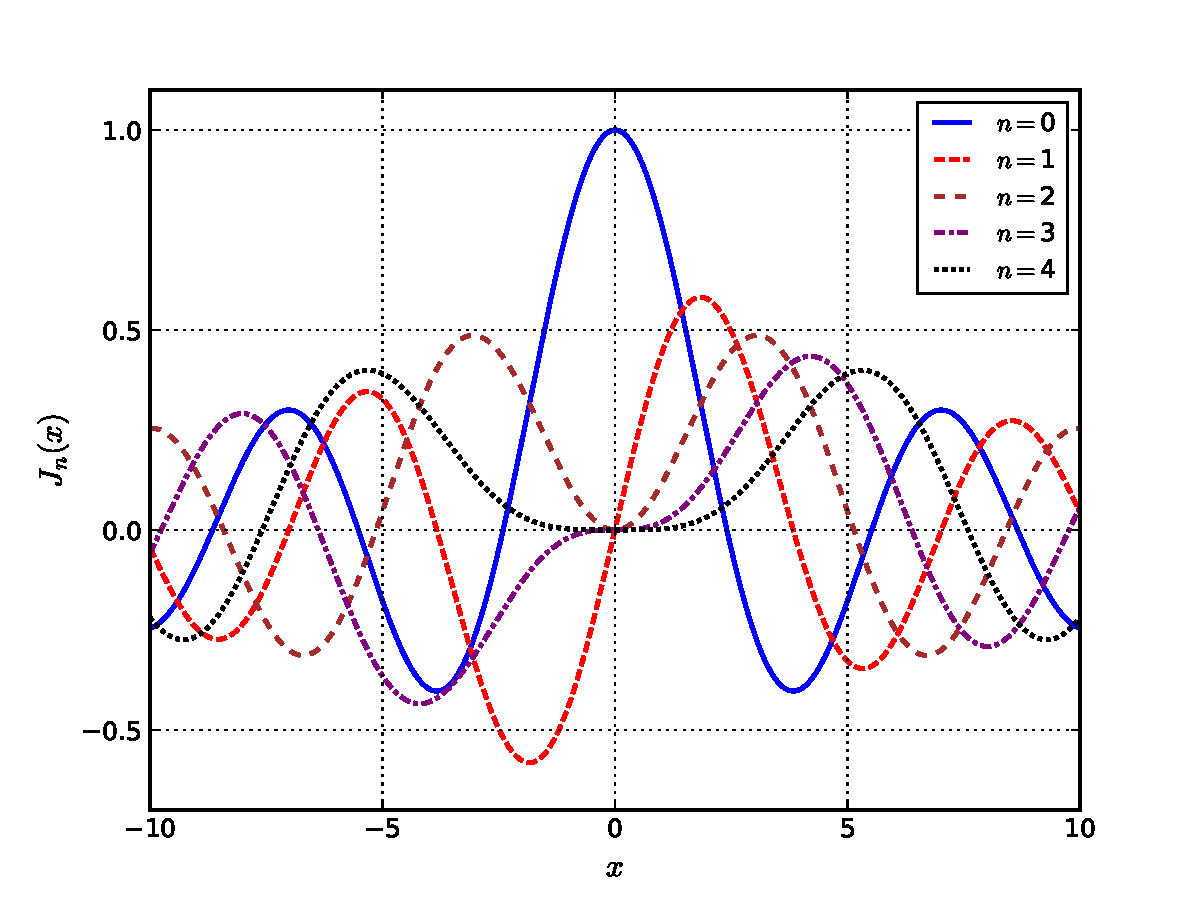
\includegraphics[angle=0,width=0.7\textwidth]{figs/fig-Bessel-J.pdf}
\caption{Primeras cinco funciones de Bessel de primera especie a orden entero.}
\label{fig-Jn}
\end{figure}
Consideremos las soluciones enteras de orden $n=0,1,2,\cdots$, entonces \eqref{Besselnu} se reduce a
\begin{align}
J_n(z) &= \sum_{k=0}^\infty \frac{(-1)^k}{k!\Gamma(k+n+ 1)}
\left(\frac{z}{2}\right)^{2k+n},
\end{align}
y como $\Gamma(k+n+ 1)$ tiene argumento entero, coincide con el factorial $(k+n)!$. Por lo tanto,
\begin{equation}
\boxed{J_n(z) =\sum_{k=0}^\infty \frac{(-1)^k}{k!(k+n)!}
\left(\frac{z}{2}\right)^{2k+n}.}
\end{equation}
Por otro lado, reemplazando $\nu=-n$, con $n=0,1,2,\cdots$, en \eqref{Besselnu} (o, equivalentemente $\nu=n$ en \eqref{J-nu}), obtenemos
\begin{align}\label{J-n}
J_{-n}(z) &= \sum_{k=0}^\infty \frac{(-1)^k}{k!\Gamma(k-n+ 1) }
\left(\frac{z}{2}\right)^{2k-n}.
\end{align}

Aqu'i hay que mirar cuidadosamente el caso en que $(k-n+ 1)$ asume valores enteros negativos, puesto que en esos casos la funci'on $\Gamma(k-n+ 1)$ diverge. Los casos en que $k-n+ 1=0,1,2,\cdots$ se presentan cuando $k=n-1,n-2,\cdots, 0$ respectivamente. Como $1/\Gamma(k-n+ 1)\to 0$ en estos casos\footnote{En otras palabras, estamos considerando (o definiendo) $J_{-n}$ como el l'imite de $J_{-\nu}$ cuando $\nu$ se acerca al entero $n$:  $J_{-n}(z):=\lim_{\nu\to n}J_{-\nu}(z)$.}, entonces los coeficientes de la suma en \eqref{J-n} tender'an a cero para todo $k=0,1,\cdots,n-1$. Por lo tanto, s'olo contribuir'an los t'erminos con $k\ge n$. Entonces \eqref{J-n} se reduce a
\begin{align}\label{J-n2}
J_{-n}(z) &= \sum_{k=n}^\infty \frac{(-1)^k}{k!\Gamma(k-n+ 1) }
\left(\frac{z}{2}\right)^{2k-n} \\
&= \sum_{k=0}^\infty \frac{(-1)^{k+n}}{(k+n)!\Gamma(k+1)}
\left(\frac{z}{2}\right)^{2k+n} \\
&= (-1)^n\sum_{k=0}^\infty \frac{(-1)^k}{(k+n)!k!}
\left(\frac{z}{2}\right)^{2k+n} \\
&= (-1)^n J_n(z).
\end{align}

Note adem'as que, como puede verse de su expresi'on en serie, las funciones $J_n(z)$ tienen paridad $n$, es decir,
\begin{equation}
J_n(-z)=(-1)^nJ_n(z).
\end{equation}

\subsection{Funci'on generadora de Funciones de Bessel de orden entero}
Consideramos la funci'on $g(t,z)$ definida por
\begin{equation}\label{defgtz}
g(t,z):=\sum_{n = -\infty}^\infty J_n(z) t^n, \qquad t,z\in \mathbb{C}.
\end{equation}
De esta forma, podemos entender a $g(t,z)$ como la \textit{funci'on generadora de las funciones de Bessel de orden entero}, por medio de la expansi'on (de Laurent) en potencias de $t$.

Para determinar la forma expl'icita de $g(t,z)$ podemos proceder como sigue. Derivamos \eqref{defgtz} con respecto a $z$ y usamos la relaci'on de recurrencia \eqref{rrJnu2} para expresar $J'_n(z)$ en t'erminos de  $J_{n-1}(z)$ y $J_{n+1}(z)$. Con esto, podemos escribir:
\begin{align}
\frac{\partial g}{\partial z} &= \sum_{n=-\infty}^\infty J'_n(z) t^n \\
&= \frac{1}{2}\sum_{n=-\infty}^\infty \left(J_{n-1}(z)-J_{n+1}(z)\right) t^n \\
&= \frac{1}{2}\left[t\sum_{n=-\infty}^\infty J_{n-1}(z)t^{n-1}-t^{-1}\sum_{n=-\infty}^\infty J_{n+1}(z)t^{n+1} \right]\\
&= \frac{1}{2}\left(t-t^{-1}\right)\sum_{n = -\infty}^\infty J_n(z) t^n\\
&= \frac{1}{2}\left(t-t^{-1}\right)g(t,z).
\end{align}
Podemos encontrar una expresi'on para la funci'on generadora a partir de esta relaci'on, consider'andola como una ecuaci'on diferencial para $g(t,z)$. La soluci'on es necesariamente de la forma
\begin{equation}\label{gtz2}
g(t,z)=f(t)\,e^{\frac{z}{2}\left(t-t^{-1}\right)}.
\end{equation}
Finalmente, la funci'on $f(t)$ puede determinarse evaluando \eqref{defgtz} para $z=0$ y luego comparando con \eqref{gtz2}:
\begin{equation}\label{gtz3}
g(t,0)=f(t)=\sum_{n = -\infty}^\infty J_n(0) t^n=J_0(0)=1.
\end{equation}
Aqu'i usamos el hecho que todas las funciones de Bessel de orden entero se anulan en $z=0$, excepto para $n=0$, ya que $J_0(0)=1$.
\begin{equation}\label{gtzJ}
\boxed{g(t,z)=e^{\frac{z}{2}\left(t-t^{-1}\right)}=\sum_{n = -\infty}^\infty J_n(z) t^n.}
\end{equation}

\subsection{Representaci'on integral}
Substituyendo $t=e^{i\theta}$ en \eqref{gtzJ} encontramos,
\begin{equation}\label{gteth}
\boxed{g(t,e^{i\theta})=e^{iz\sen\theta}=\sum_{n = -\infty}^\infty J_n(z) e^{in\theta}.}
\end{equation}
Esto significa que las \textit{funciones de Bessel son los coeficientes de la expansi'on en serie de Fourier de la funci'on} $e^{iz\sen\theta}$. Por lo tanto,
\begin{equation}
\boxed{J_n(z)=\frac{1}{2\pi}\int_0^{2\pi}e^{iz\sen\theta}e^{-in\theta}\,d\theta.}
\end{equation}
Equivalentemente, ya que el integrando es peri'odico de periodo $2\pi$, podemos desplazar el intervalo de integraci'on a $[-\pi,\pi]$, y escribir
\begin{equation}
J_n(z)=\frac{1}{2\pi}\int_{-\pi}^{\pi}e^{i(z\sen\theta-n\theta)}\,d\theta.
\end{equation}
Como $e^{i(z\sen\theta-n\theta)}=\cos(z\sen\theta-n\theta)+i\sen(z\sen\theta-n\theta)$, vemos que el integrando se divide en una contribuci'on par y otra impar en $\theta$. Por lo tanto,
\begin{equation}
\boxed{J_n(z)=\frac{1}{\pi}\int_0^{\pi}\cos(z\sen\theta-n\theta)\,d\theta.}
\end{equation}
En particular,
\begin{equation}
\boxed{J_0(z)=\frac{1}{2\pi}\int_{-\pi}^{\pi}e^{iz\sen\theta}\,d\theta=\frac{1}{\pi}\int_0^{\pi}\cos(z\sen\theta)\,d\theta.}
\end{equation}

\subsection{Sumatorias de funciones de Bessel}

Adicionalmente, de la relaci'on \eqref{gteth} podemos escribir,
\begin{align}
e^{iz\sen\theta} &= J_0(z)+\sum_{n=1}^\infty\left(J_n(z) e^{in\theta}+J_{-n}(z) e^{-in\theta}\right) \\
&=  J_0(z)+\sum_{n=1}^\infty\left(J_n(z) e^{in\theta}+(-1)^nJ_{n}(z) e^{-in\theta}\right) \\
&=  J_0(z)+\sum_{\substack{n=1 \\ n \text{ impar}}}^\infty J_n(z)\left(e^{in\theta}-e^{-in\theta}\right)+\sum_{\substack{n=2 \\ n \text{ par}}}^\infty J_n(z)\left(e^{in\theta}+e^{-in\theta}\right) \\
&=  J_0(z)+2i\sum_{\substack{n=1 \\ n \text{ impar}}}^\infty J_n(z)\sen(n\theta) +2\sum_{\substack{n=2 \\ n \text{ par}}}^\infty J_n(z)\cos(n\theta) \\
&=  J_0(z)+2i\sum_{n=1}^\infty J_{2n-1}(z)\sen[(2n-1)\theta] +2\sum_{n=1}^\infty J_{2n}(z)\cos(2n\theta).
\end{align}
Si el argumento de las funciones es real ($z=x$) entonces, igualando la parte real e imaginaria de ambos lados de la igualdad, obtenemos
\begin{equation}
\boxed{\cos(x\sen\theta)=J_0(x)+2\sum_{n=1}^\infty J_{2n}(x)\cos(2n\theta),}
\end{equation}
\begin{equation}
\boxed{\sen(x\sen\theta)=2\sum_{n=1}^\infty J_{2n-1}(x)\sen[(2n-1)\theta].}
\end{equation}

En particular, si $\theta=0$, obtenemos la relaci'on
\begin{equation}
J_0(x)+2\sum_{n=1}^\infty J_{2n}(x)=1.
\end{equation}

\section{Funciones de Bessel de orden semi-entero}
\begin{align}
J_{1/2}(z) &= \sum_{k=0}^\infty\frac{(-1)^k}{k!\Gamma(k+1/2+1)}
\left(\frac{z}{2}\right)^{2k+1/2} \\
&= \sum_{k=0}^\infty\frac{(-1)^k}{k!\Gamma(k+3/2)}
\left(\frac{z}{2}\right)^{2k+1/2} \\
&= \left(\frac{2}{\pi z}\right)^{1/2} \sum_{k=0}^\infty \frac{(-1)^k}
{(2k+1)!} z^{2k+1} \\
&= \left(\frac{2}{\pi z}\right)^{1/2} \sen z. \label{J1/2}
\end{align}
Aqu'i hemos usado
\begin{align}
\Gamma(k+\frac{3}{2}) &= (k+\frac{1}{2})\Gamma(k+\frac{1}{2}) \\
&= (k+\frac{1}{2})(k-\frac{1}{2})\Gamma(k-\frac{1}{2}) \\
&=  (k+\frac{1}{2})(k-\frac{1}{2})(k-\frac{3}{2})\Gamma(k-\frac{3}{2}) \\
&= \quad \cdots \\
&=  (k+\frac{1}{2})(k-\frac{1}{2})(k-\frac{3}{2})\frac{1}{2}\Gamma(\frac{1}{2}) \\
&= \frac{\sqrt{\pi}}{2^{k+1}} \underbrace{1\cdot 3\cdot 5\cdots (2k-1)(2k+1)}_{k+1\text{ t'erminos}} \\
&= \frac{\sqrt{\pi}}{2^{2k+1}}\frac{(2k+1)!}{k!}.
\end{align}

An'alogamente,
\begin{align}
J_{-1/2}(z) &= \sum_{k=0}^\infty\frac{(-1)^k}{k!\Gamma(k-1/2+1)}
\left(\frac{z}{2}\right)^{2k+1/2} \\
&= \sum_{k=0}^\infty\frac{(-1)^k}{k!\Gamma(k+1/2)}
\left(\frac{z}{2}\right)^{2k+1/2} \\
&= \left(\frac{2}{\pi z}\right)^{1/2} \sum_{k=0}^\infty \frac{(-1)^k}
{(2k)!} z^{2k} \\
&= \left(\frac{2}{\pi z}\right)^{1/2} \cos z, \label{J-1/2}
\end{align}
ya que
\begin{align}
\Gamma(k+\frac{1}{2}) &= \frac{\Gamma(k+\frac{3}{2})}{(k+\frac{1}{2}}) \\
&= \frac{\sqrt{\pi}}{2^{2k+1}}\frac{(2k+1)!}{(k+\frac{1}{2})k!}\\
&= \frac{\sqrt{\pi}}{2^{2k}}\frac{(2k)!}{k!}.
\end{align}

Podemos encontrar las otras funciones de Bessel de orden semi-entero usando las relaciones de recurrencia \eqref{rrJnu1} y \eqref{rrJnu2}. Por ejemplo
\begin{align}
    J_{3/2}(z)
    &= \frac{(1/2)}{z} J_{1/2}(z) - J_{1/2}'(z) 
    \\
    &= \frac{1}{2z} \left( \frac{2}{\pi} \right)^{1/2} z^{-1/2} \sen z
    - \left(-\frac{1}{2}\right) \left(\frac{2}{\pi}\right)^{1/2}
    z^{-3/2} \sen z - \left(\frac{2}{\pi}\right)^{1/2} z^{-1/2}
    \cos z 
    \\
    &= 2^{-1/2} \pi^{-1/2} z^{-3/2} \sen z
    + 2^{-1/2} \pi^{-1/2} z^{-3/2} \sen z
    - 2^{-1/2} \pi^{-1/2} \cos z 
    \\
    &= \left(\frac{2}{\pi}\right)^{1/2} z^{-3/2} \sen z
    - \left(\frac{2}{\pi}\right)^{1/2} z^{-1/2} \cos z 
    \\
    &= \left(\frac{2}{\pi}\right)^{1/2} \left( z^{-3/2} \sen z
      - z^{-1/2} \cos z \right).
  \end{align}



\section{Funciones de Bessel de segunda especie}\label{sec:FB2E}
Como hemos ya discutido en la secci'on \ref{secsolBess}, cuando $\nu$ no es un entero, las funciones de Bessel de segunda especie, tambi'en llamadas funciones de Neumann $N_\nu(z)$ ('o $Y_\nu(z)$), definidas por
\begin{equation}\label{defNnu}
N_\nu (z):=  \frac{J_\nu(z) \cos(\nu \pi) - J_{-\nu}(z)}{\sen(\nu \pi)} , \qquad \nu\neq n=0, \pm 1, \pm, 2, \cdots,
\end{equation}
son soluciones linealmente independientes de $J_\nu(z)$ de ecuaci'on de Bessel. Esta combinaci'on lineal particular es 'util puesto que, entre otras cosas, suministra una expresi'on complementaria a las funciones $J_\nu(z)$ en lo que respecta a su forma asint'otica. En efecto, a partir de \eqref{asinJnu} encontramos que
\begin{equation}\label{asinNnu}
\boxed{N_\nu(x)\approx \sqrt{\frac{2}{\pi x}}\sen\left(x-\frac{\nu\pi}{2}-\frac{\pi}{4}\right), 
\qquad x\gg\left|\nu^2-\frac{1}{4}\right|.}
\end{equation}
Adem'as, puede usarse la misma expresi'on \eqref{defNnu} en el caso en que $\nu$ es entero ($\nu=n$). Sabemos que en este caso, $J_{-n}(z)$ no es linealmente independiente de $J_{-n}(z)$ ya que se cumple que $J_{-n}(z)=(-1)^nJ_n(z)$. No obstante, podemos usar \eqref{defNnu} para encontrar la segunda soluci'on linealmente independiente $N_n(z)$, \textit{como el l'imite de \eqref{defNnu} cuando el par'ametro $\nu$ se acerca al entero $n$}, es decir,
\begin{equation}\label{Nnlim}
N_n(z):=  \lim_{\nu\to n}\frac{J_\nu(z) \cos(\nu \pi) - J_{-\nu}(z)}{\sen(\nu \pi)} , \qquad n=0, \pm 1, \pm, 2, \cdots .
\end{equation}
Note que los coeficientes de la combinaci'on lineal \eqref{defNnu} son tales que el l'imite es no trivial, ya que tanto el numerador como el denominador tienden a cero cuando $\nu$ tiende a $n$. Por esto, usando la regla de L'H\^opital, encontramos que
\begin{equation}\label{Nnder}
N_n(z)=\frac{1}{\pi}\left[\frac{\partial J_\nu(z)}{\partial\nu}-(-1)^n\frac{\partial J_{-\nu}(z)}{\partial\nu}\right]_{\nu=n}.
\end{equation}
Puede (h'agalo!) verificarse que la funci'on definida por \eqref{Nnder}, efectivamente satisface la ecuaci'on de Bessel \eqref{Besselec1}. Adem'as, de \eqref{Nnder} se sigue, usando $(\partial J_\nu/\partial\nu)_{\nu=-n}=-(\partial J_{-\nu}/\partial\nu)_{\nu=n}$, que
\begin{equation}
\boxed{N_{-n}(z)=(-1)^nN_n(z).}
\end{equation}
Por otro lado, de la expansi'on \eqref{J-nu} obtenemos que cerca de $z=0$, y para $\nu>0$,
\begin{equation}
N_\nu(z)\approx -\frac{1}{\sen(\nu\pi)}\frac{1}{\Gamma(1-\nu)}\left(\frac{2}{z}\right)^\nu=-\frac{1}{\pi}\Gamma{(\nu)}\left(\frac{2}{z}\right)^\nu.
\end{equation}
Aqu'i hemos usamos la identidad \eqref{GzG1-z}. Por lo tanto, para $\nu\to n$, obtenemos
\begin{equation}
N_n(z)\approx -\frac{1}{\pi}(n-1)!\left(\frac{2}{z}\right)^n, \qquad z\approx 0, \qquad n>0,
\end{equation}
de donde vemos que estas funciones divergen en el origen origen. Note que incluso $N_0(z)$ diverge en $z=0$, ya que\footnote{A partir de \eqref{Nnder}, se encuentra, usando la \textit{funci'on  digamma} $\Psi_0(z):=\Gamma'(z)/\Gamma(z)$, que: \begin{equation}
N_0(z)=\frac{2}{\pi}\left(\frac{\partial J_\nu}{\partial\nu}\right)_{\nu=0}=\frac{2}{\pi}\left[-\frac{\Psi_0(\nu+1)}{\Gamma(\nu+1)}\left(\frac{z}{2}\right)^\nu+\frac{1}{\Gamma(\nu+1)}\left(\frac{z}{2}\right)^\nu\ln\left(\frac{z}{2}\right)+\cdots\right]_{\nu=0}=\frac{2}{\pi}\left[-\Psi_0(1)+\ln\left(\frac{z}{2}\right)+\cdots\right].
\end{equation}}  
\begin{equation}
N_0(z)\approx \frac{2}{\pi}\left[\ln\left(\frac{z}{2}\right) + \gamma \right], \qquad z\approx 0,	
\end{equation}
donde $\gamma=-\Psi_0(1)$ es la constante de Euler-Mascheroni, $\gamma=0.5772\cdots$.


\subsection{Representaci'on integral}
\begin{equation}
N_n(x) =\frac{1}{\pi} \int_0^\pi \sen(x \sen\theta - n\theta) \, d\theta
- \frac{1}{\pi} \int_0^\infty\left[ e^{n t} + (-1)^n e^{-n t} \right]
 e^{-x \senh t} \, dt.
\end{equation}


\subsection{Relaciones de Recurrencia}
A partir de la definici'on \eqref{Nnlim} y las relaciones de recurrencia para las funciones de Bessel \eqref{rrJnu1} y \eqref{rrJnu2}, puede verificarse que las funciones de Bessel de segunda especie satisfacen \textit{las mismas relaciones de recurrencia que las de primera especie}:
\begin{equation}\label{rrNnu1}
N_{\nu-1}(z)+N_{\nu+1}(z)=\frac{2\nu}{z}N_\nu(z),
\end{equation}
\begin{equation}\label{rrNnu2}
N_{\nu-1}(z)-N_{\nu+1}(z)=2N'_\nu(z).
\end{equation}



\begin{figure}[H]
\centering
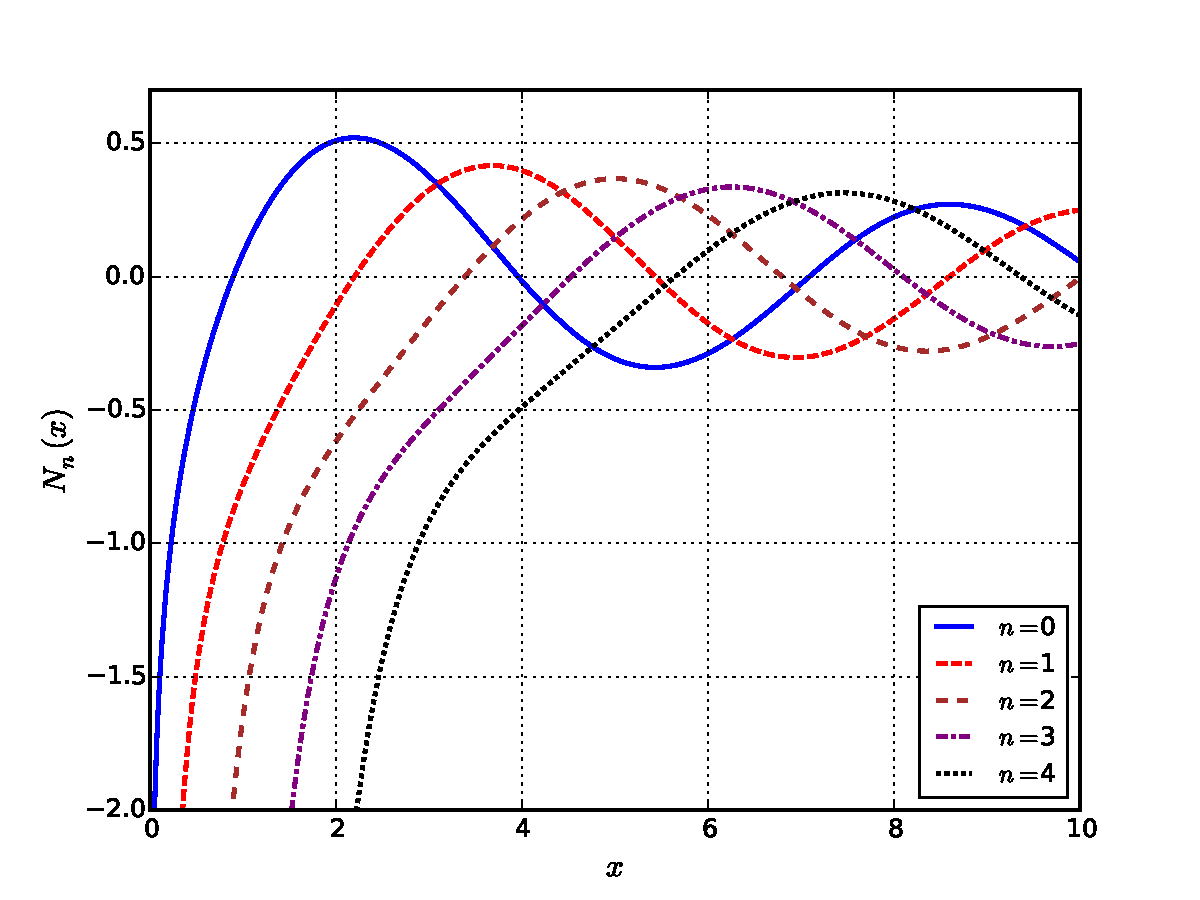
\includegraphics[angle=0,width=0.7\textwidth]{figs/fig-Bessel-N.pdf}
\caption{Primeras cinco funciones de Bessel de segunda especie (funciones de Neumann) de orden entero.}
\label{fig-Nn}
\end{figure}

\section{Funciones de Hankel}
En muchas aplicaciones f'isicas (especialmente cuando se estudian soluciones de la ecuaci'on de onda) es conveniente introducir otro par de funciones linealmente independientes, llamadas funciones de Hankel y denotadas por $H_\nu^{(1)}$ y $H_\nu^{(2)}$, definidas por
\begin{align}
  H_\nu^{(1)}(z) &:= J_\nu(z) + i N_\nu(z),  \\
  H_\nu^{(2)}(z) &:= J_\nu(z) - i N_\nu(z) .
\end{align}
%Wronskiano:
%\begin{equation} 
%W[H_\nu^{(1)}, H_\nu^{(2)}] = - \frac{i 4}{\pi z}. 
%\end{equation}
Las funciones de Hankel son linealmente independientes para todo $\nu$, y satisfacen las mismas relaciones de recurrencia que las funciones de Bessel.
La utilidad de su definici'on resulta clara al considerar su forma asint'otica. Usando \eqref{asinJnu} y \eqref{asinNnu} se encuentra que
\begin{equation}
H_\nu^{(1)}(x)\approx \sqrt{\frac{2}{\pi x}}\,e^{i(x-\nu\pi/2-\pi/4)}, \quad 
H_\nu^{(2)}(x)\approx \sqrt{\frac{2}{\pi x}}\,e^{-i(x-\nu\pi/2-\pi/4)}, 
\quad x\gg\left|\nu^2-\frac{\pi}{4}\right|.
\end{equation}

%\begin{align}
%H_\nu^{(1)}(x) &= \frac{e^{-\frac{1}{2} \nu\pi i}}{\pi i}\int_{-\infty}^{+\infty} e^{ix\cosh t - \nu t} \, dt, \\
%H_\nu^{(2)}(x) &= -\frac{e^{-\frac{1}{2} \nu\pi i}}{\pi i}\int_{-\infty}^{+\infty} e^{-ix\cosh t - \nu t} \, dt.
%\end{align}

\section{Funciones modificadas de Bessel}
La \textit{ecuaci'on modificada de Bessel} es 
\begin{equation} 
y'' + \frac{1}{x}y' -\left(1+\frac{\nu^2}{x^2}\right)y(x) = 0. 
\end{equation}
Las soluciones finitas en $x=0$ de esta ecuaci'on son de la forma $y(x)=J_\nu(ix)$. Como estamos especialmente interesados en el caso en que tanto $x$ como $y$ son reales, es conveniente  definir las \textit{funciones modificadas de Bessel de primera especia y orden} $\nu$:
\begin{equation}\label{defInu}
I_\nu(x) = i^{-\nu} J_\nu(ix). 
\end{equation}
La funci'on $I_\nu(x)$ as'i definida es real. En efecto, de la expansi'on en serie \eqref{Besselnu}
\begin{align}
  I_\nu(x) &= i^{-\nu} J_\nu(ix)   \\
  &= i^{-\nu}\sum_{k=0}^\infty\frac{(-1)^k}{k!\Gamma(k+\nu+1)}
  \left(\frac{ix}{2}\right)^{2k+\nu} \\
  &= i^{-\nu} \sum_{k=0}^\infty \frac{(-1)^k i^\nu i^{2k}}{k!\Gamma(k+\nu+1)} 
  \left(\frac{x}{2}\right)^{2+\nu}.
\end{align}
Por lo tanto,
\begin{equation}
\boxed{I_\nu(x) = \sum_{k=0}^\infty\frac{1}{k!\Gamma(k+\nu+ 1)}
  \left(\frac{x}{2}\right)^{2k+\nu}.}
\end{equation}
Nuevamente, $I_\nu$ y $I_{-\nu}$ son linealmente independientes, excepto si $\nu$ es entero, ya que en este 'ultimo caso se satisface que
\begin{equation}
I_{-n}(x)=I_n(z)
\end{equation}
\begin{figure}[H]
\centering
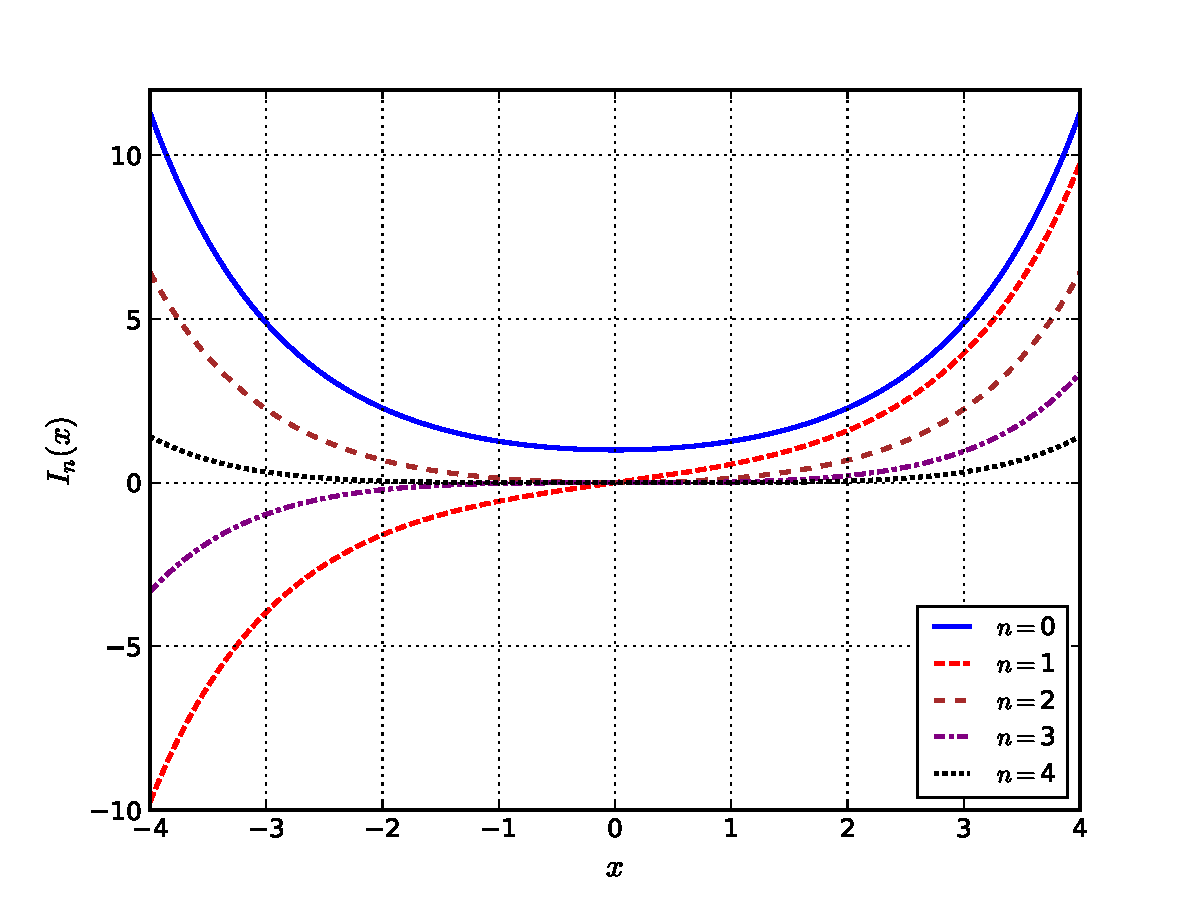
\includegraphics[angle=0,width=0.7\textwidth]{figs/fig-Bessel-I.pdf}
\caption{Primeras cinco funciones modificadas de Bessel (de primera especie) de orden entero.}
\label{fig-In}
\end{figure}
La correspondiente forma asint'otica de las funciones modificadas de Bessel $I_\nu(x)$ es
\begin{equation}
I_\nu(x) \approx \frac{1}{\sqrt{2\pi x}}\,e^x, \qquad x\gg\left|\nu^2-\frac{1}{4}\right|.
\end{equation}

Las funciones $I_\nu(x)$ satisfacen las siguientes relaciones de recurrencia, que se siguen a partir de \eqref{rrJnu1}, \eqref{rrJnu2} y \eqref{defInu}:
\begin{equation}\label{rrInu1}
I_{\nu-1}(x)+I_{\nu+1}(x)=2I'_\nu(x),
\end{equation}
\begin{equation}\label{rrInu2}
I_{\nu-1}(x)-I_{\nu+1}(x)=\frac{2\nu}{x}I_\nu(x).
\end{equation}

\subsection{Funciones Modificadas de Bessel de segunda especie}
En analog'ia con lo visto en la secci'on \ref{sec:FB2E}, es conveniente introducir las funciones de segunda especie, ahora denotadas por $K_\nu(x)$, y definidas de la forma siguiente:
\begin{equation}\label{defKnu}
K_\nu(x) := \frac{\pi}{2}\left[\frac{I_{-\nu}(x)-I_\nu(x)}{\sen(\nu\pi)}\right], \qquad \nu\neq n=0,\pm 1,\pm 2, \cdots.
\end{equation}
Note que como consecuencia de esta definici'on $K_{-\nu}(x)=K_\nu(x)$, por lo que es suficiente considerar $\nu\ge 0$.
Con estas definiciones, $I_\nu$ y $K_\nu$ son l.i. para todo $\nu$, y su forma asint'otica es nuevamente ``complementaria'' ya que
\begin{equation}
K_\nu(x) \approx \sqrt{\frac{\pi}{2x}} e^{-x}.
\end{equation}

En el caso de $\nu$ entero, la definici'on se realiza como el l'imite $\nu\to n$, es decir,
\begin{equation}
K_n(x) := \lim_{\nu\to n}\frac{\pi}{2}\left[\frac{I_{-\nu}(x)-I_\nu(x)}{\sen(\nu\pi)}\right], \qquad  n=0,1,2, \cdots.
\end{equation}
Usando nuevamente la regla de L'H\^opital, podemos escribir
\begin{equation}\label{Knder}
K_n(x)=\frac{(-1)^n}{2}\left[\frac{\partial I_{-\nu}(x)}{\partial\nu}-\frac{\partial I_\nu(x)}{\partial\nu}\right]_{\nu=n}.
\end{equation}

\begin{figure}[H]
\centering
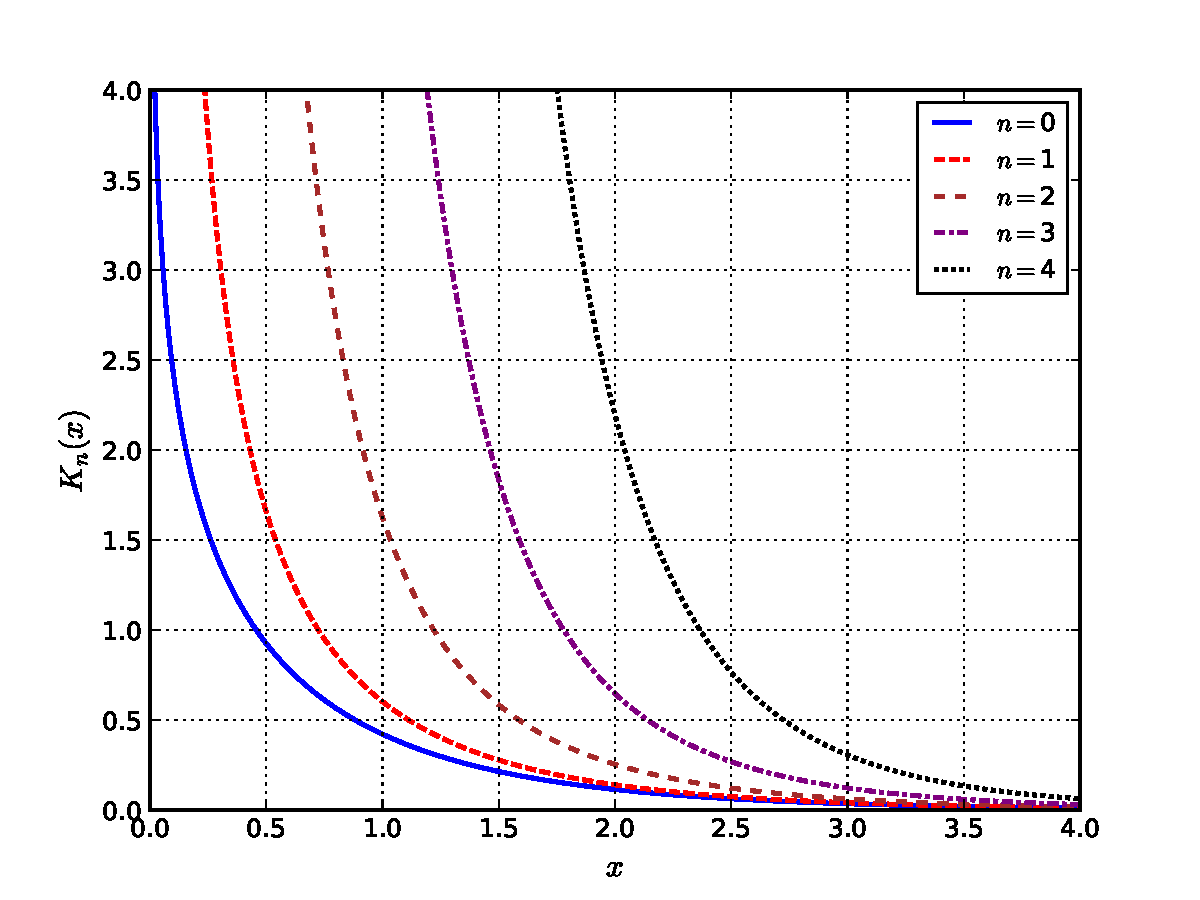
\includegraphics[angle=0,width=0.7\textwidth]{figs/fig-Bessel-K.pdf}
\caption{Primeras cinco funciones modificadas de Bessel de segunda primera especie y orden entero.}
\label{fig-Kn}
\end{figure}
Las funciones $K_\nu(x)$ satisfacen las siguientes relaciones de recurrencia
\begin{equation}\label{rrKnu1}
K_{\nu-1}(x)+K_{\nu+1}(x)=-2K'_\nu(x),
\end{equation}
\begin{equation}\label{rrKnu2}
K_{\nu-1}(x)-K_{\nu+1}(x)=-\frac{2\nu}{x}K_\nu(x),
\end{equation}
como puede verificarse a partir de \eqref{rrInu1}, \eqref{rrInu2}, \eqref{defKnu} y \eqref{Knder}. Note la diferencia de signo de estas relaciones con respecto a las correspondientes a las funciones de primera especie, \eqref{rrInu1} y \eqref{rrInu2}.

\section{Funciones Esf'ericas de Bessel}
Como vimos, en coordenadas esf'ericas la ecuaci'on radial proveniente de la separaci'on de variables de la ecuaci'on de Helmholtz es \eqref{ecrHelmce}. Adem'as, las soluciones finitas en $\theta=0$ y $\theta=\pi$ (es decir, sobre el eje $z$) de \eqref{ecThHelm} requieren que $Q=n(n+1)$. La ecuaci'on resultante tiene entonces soluciones de la forma
%\begin{equation}
%x^2 \frac{d^2 y}{dx^2} + 2x \frac{dy}{dx} + [x^2 - n(n+1)]y = 0.
%\end{equation}
\begin{equation}
R_n(r) = \frac{u_n(kr)}{\sqrt{r}} ,
\end{equation}
donde $k=\sqrt{|\alpha|}$ y $u_n(x)$ es soluci'on de la ecuaci'on (modificada, si $\alpha<0$) de Bessel de orden semientero, $\nu=n+1/2$.

En el caso en que $\alpha>0$, las soluciones $u(x)$ ser'an entonces combinaciones de funciones de Bessel de primera y segunda especie. Por esto, es conveniente definir las funciones esf'ericas de Bessel (de primera y segunda especie) por:
\begin{equation}
j_{n}(x) := \sqrt{\frac{\pi}{2x}} J_{n+1/2}(x),
\end{equation}
\begin{equation}
n_{n}(x) := \sqrt{\frac{\pi}{2x}} N_{n+1/2}(x) = (-1)^{n+1} \sqrt{\frac{\pi}{2x}} J_{-n-1/2}(x).
\end{equation}
El factor $\sqrt{\pi/2}$ es incluido por conveniencia, ya que entonces (ver \eqref{J1/2} y \eqref{J-1/2}) las primeras funciones resultan ser simples:
\begin{equation}\label{j0n0}
j_0(x) = \frac{\sen x}{x}, \qquad n_0(x)=-\,\frac{\cos x} {x}.
\end{equation}
Podemos encontrar una expresi'on en serie simple a partir\footnote{y usando la ``f'ormula de duplicaci'on de Legendre'', ver por ejemnplo ec. (10.66b) de \cite{Arfken}: $\Gamma(z+1)\Gamma(z+1/2)\equiv 2^{-2z}\pi^{1/2}\Gamma(2z+1)$, con $z=k+n+1/2$.} de \eqref{Besselnu},
\begin{align}
J_{n+1/2} (x)&= \sum_{k = 0}^\infty \frac{ (-1)^k }{ k! \Gamma(k + n + 3/2) }
\left( \frac{x}{2} \right)^{2k+n+1/2} \\
&=\sqrt{\frac{x}{2}} \sum_{k=0}^\infty \frac{ (-1)^k }{ k! \Gamma(k + n + 3/2) }
\left( \frac{x}{2} \right)^{2k+n} \\
&=\sqrt{\frac{x}{2}} \sum_{k=0}^\infty \frac{ (-1)^k }{ k!}\frac{2^{2k+2n+1}\Gamma(k+n+1)}{\pi^{1/2}\Gamma(2k+2n+2)}
\left( \frac{x}{2} \right)^{2k+n} \\
&=\sqrt{\frac{2x}{\pi}} 2^{2n}\sum_{k=0}^\infty \frac{(-1)^k }{k!}\frac{2^{2k}(k+n)!}{(2k+2n+1)!}\left(\frac{x}{2}\right)^{2k+n} \\
&=\sqrt{\frac{2x}{\pi}} 2^n x^n\sum_{k=0}^\infty \frac{(-1)^k}{k!}\frac{(k+n)!}{(2k+2n+1)!}x^{2k} .
\end{align}
Por lo tanto,
\begin{equation}
\boxed{j_n(x)=2^n x^n\sum_{k=0}^\infty \frac{(-1)^k}{k!}\frac{(k+n)!}{(2k+2n+1)!}x^{2k} .}
\end{equation}

An'alogamente, para la funci'on esf'erica de segunda especie, encontramos
\begin{equation}
\boxed{n_n(x)=\frac{(-1)^{n+1}}{2^nx^{n+1}}\sum_{k=0}^\infty \frac{(-1)^k(k-n)!}{k!(2k-2n)!}x^{2k} .}
\end{equation}

\subsection{Relaciones de Recurrencia}
A partir de las relaciones de recurrencia para $J_\nu$ y $N_\nu$, ver \eqref{rrJnu1}, \eqref{rrJnu2}, \eqref{rrNnu1} y \eqref{rrNnu2}, podemos derivar directamente las correspondientes relaciones para las funciones esf'ericas, obteniendo:
\begin{equation}
j_{n-1}(x)+j_{n+1}(x)=\frac{2n+1}{x}j_n(x), \qquad nj_{n-1}(x)-(n+1)j_{n+1}(x)=(2n+1)j'_n(x).
\end{equation}
Similarmente \eqref{Jnu-1JpJ2} y \eqref{rrJni+2} implican que
\begin{equation}
j_{n-1}(x)=x^{-n-1}\frac{d\ }{dx}\left[x^{n+1}j_n(x)\right],
\end{equation}
\begin{equation}\label{jn+1jn}
j_{n+1}(x)=-x^{n}\frac{d\ }{dx}\left[x^{-n}j_n(x)\right].
\end{equation}
Aplicando sucesivamente \eqref{jn+1jn} obtenemos una expresi'on en t'erminos de la funci'on $j_0(x)$:
\begin{equation}
j_n(x) = (-x)^n \left(\frac{1}{x}\frac{d}{dx}\right)^n\,j_0(x) .
\end{equation}
Similarmente,
\begin{equation}
n_n(x) = (-x)^n \left(\frac{1}{x}\frac{d}{dx}\right)^n\,n_0(x).
\end{equation}

\subsection{Expresiones expl'icitas}

De este modo, usando \eqref{j0n0} encontramos las siguientes 'utiles expresiones:
\begin{equation}
\boxed{j_n(x) = (-x)^n \left(\frac{1}{x}\frac{d}{dx}\right)^n\,\frac{\sen x}{x},}
\end{equation}
\begin{equation}
\boxed{n_n(x) = -(-x)^n \left(\frac{1}{x}\frac{d}{dx}\right)^n\,\frac{\cos x}{x}.}
\end{equation}
De este modo, podemos calcular expl'icitamente las funciones que necesitemos. Por ejemplo:
\begin{align}
j_0(x) &= \frac{\sen x}{x}, \\
j_1(x) &= \frac{\sen x} {x^2}- \frac{\cos x} {x}, \\
j_2(x) &= \left(\frac{3} {x^2} - 1 \right)\frac{\sen x}{x} - \frac{3\cos x} {x^2}, \\
j_3(x) &= \left(\frac{15}{x^3} - \frac{6}{x} \right)\frac{\sen x}{x} -\left(\frac{15}{x^2} - 1\right) \frac{\cos x} {x},
\end{align}
\begin{align}
n_0(x) &= -j_{-1}(x)=-\,\frac{\cos x} {x} ,\\
n_1(x) &= j_{-2}(x)=-\,\frac{\cos x} {x^2}- \frac{\sen x} {x}, \\
n_2(x) &=-j_{-3}(x)=\left(-\,\frac{3}{x^2}+1 \right)\frac{\cos x}{x}- \frac{3 \sen x} {x^2}, \\
n_{3}(x) &= j_{-4}(x) =\left( -\frac{15}{x^{3}}+\frac{6}{x}\right) \frac{\cos
x}{x}-\left( \frac{15}{x^{2}}-1\right) \frac{\sen x}{x}.
\end{align}
\begin{figure}[H]
\centering
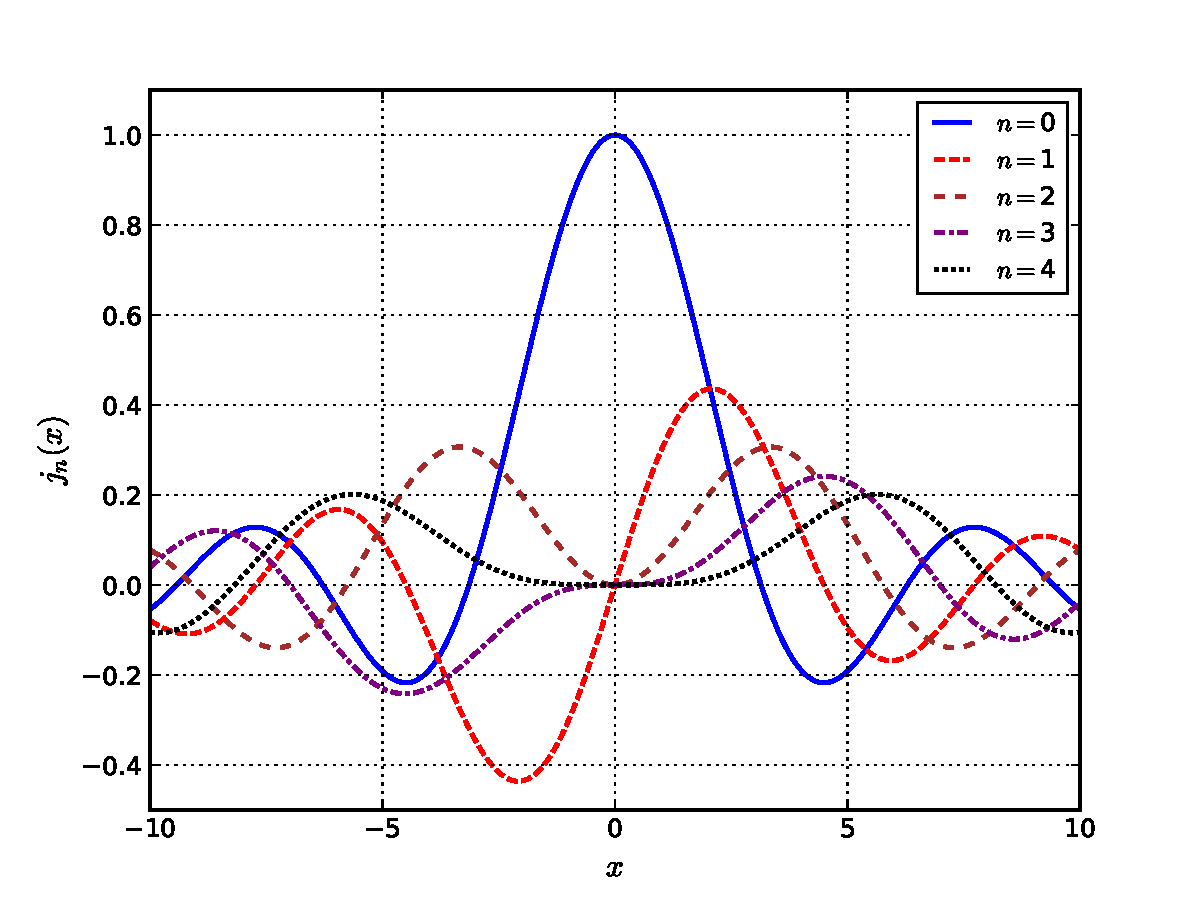
\includegraphics[angle=0,width=0.7\textwidth]{figs/fig-Bessel-Esferica-j.pdf}
\caption{Primeras cinco funciones esf'ericas de Bessel de primera especie de orden entero.}
\label{fig-jn}
\end{figure}
%
\begin{figure}[H]
\centering
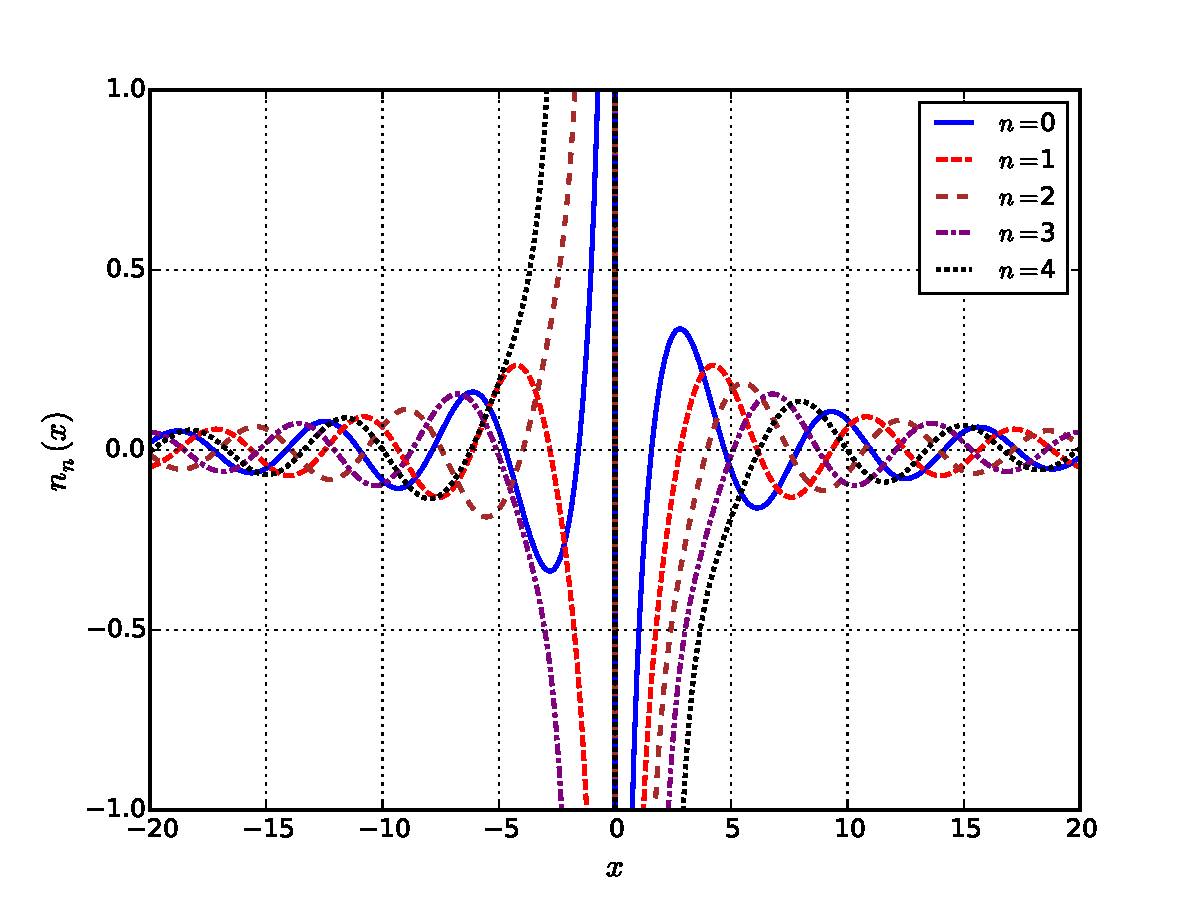
\includegraphics[angle=0,width=0.7\textwidth]{figs/fig-Bessel-Esferica-n.pdf}
\caption{Primeras cinco funciones esf'ericas de Bessel de segunda especie (funciones de Newmann) de orden entero.}
\label{fig-nn}
\end{figure}


\subsection{Relaciones de Ortogonalidad}
Nuevamente, podemos encontrar relaciones v'alidas para las funciones esf'ericas a partir de aquellas derivadas para las funciones de Bessel $J_\nu$. A partir de \eqref{roJnualpha} se sigue directamente que
\begin{equation}\label{rojnualpha}
\boxed{\int_0^a j_n\left(\frac{\bar{\alpha}_{n,m}}{a}r\right)j_n\left(\frac{\bar{\alpha}_{n,m'}}{a}r\right)r^2\,dr
=\delta_{m,m'}\frac{a^3}{2}\left[j_{n+1}(\bar{\alpha}_{n,m})\right]^2,}
\end{equation}
donde $\bar{\alpha}_{n,m}$ denota la $m$-'esima raiz de la la funci'on esf'erica $j_n(x)$. Ya que $j_n$ es proporcional a $J_{n+1/2}$, entonces $\bar{\alpha}_{n,m}=\alpha_{n+1/2,m}$.


\subsection{Funciones esf'ericas de Hankel} 
\begin{align}
h_n^{(1)}(x) &= j_n(x) + i n_n(x) , \\
h_n^{(2)}(x) &= j_n(x) - i n_n(x).
\end{align}
\begin{equation}
h_n^{(1)}(x) = (-i)^{n+1} \frac{e^{ix}}{x} \sum_{m=0}^n \frac{i^m}{m!(2x)^m} \frac{(n+m)!}{(n-m)!}
\end{equation}

\subsection{Forma asint'otica}
Para $x\ll 1$,
\begin{align}
j_n(x) &\approx \frac{2^nn!}{(2n+1)!}x^n, \\
n_n(x) &\approx -\frac{(2n)!}{2^nn!}\frac{1}{x^{n+1}}.
\end{align}
Para $x\gg n(n+1)$,
\begin{align}
j_n(x) &\approx \frac{1}{x}\sen\left(x-\frac{n\pi}{2}\right), \\
n_n(x) &\approx -\frac{1}{x}\cos\left(x-\frac{n\pi}{2}\right), \\
h^{(1)}_n(x) &\approx -\frac{i}{x}e^{i(x-{n\pi}/{2})}=(-i)^{n+1}\frac{e^{ix}}{x}, \\
h^{(2)}_n(x) &\approx \frac{i}{x}e^{-i(x-{n\pi}/{2})}=(i)^{n+1}\frac{e^{-ix}}{x}.
\end{align}

\subsection{Funciones modificadas esf'ericas de Bessel}
\begin{equation}
i_n(x):=i^{-n}j_n(ix)=\sqrt{\frac{\pi}{2x}}I_{n+1/2}(x), \qquad 
k_n(x):=-i^{n}h^{(1)}(ix)=\sqrt{\frac{\pi}{2x}}K_{n+1/2}(x).
\end{equation}

\subsubsection{Relaciones de Recurrencia}
\begin{align}
i_{n-1}(x)-i_{n+1}(x) &= \frac{2n+1}{x}i_n(x),  \\
ni_{n-1}(x)+(n+1)i_{n+1}(x) &= (2n+1)i'_n(x),
\end{align}
\begin{align}
k_{n-1}(x)-k_{n+1}(x) &= -\frac{2n+1}{x}k_n(x),\\
nk_{n-1}(x)+(n+1)k_{n+1}(x) &= -(2n+1)k'_n(x),
\end{align}
\begin{equation}
i_{n+1}(x)=x^n\frac{d\ }{dx}(x^{-n}i_n), \qquad k_{n+1}(x)=-x^n\frac{d\ }{dx}(x^{-n}k_n).
\end{equation}


\subsubsection{Formas asint'oticas}
\begin{equation}
i_n(x)\approx\frac{2^nn!}{(2n+1)!}x^n, \qquad k_n(x)\approx\frac{(2n)!}{2^nn!}x^{-n-1}, \qquad x\ll 1,
\end{equation}
\begin{equation}
i_n(x)\approx \frac{e^x}{2x}, \qquad k_n(x)\approx \frac{-e^x}{x}, \qquad x\gg \frac{n(n+1)}{2}.
\end{equation}


\subsubsection{Expresiones expl'icitas}
\begin{equation}
i_n(x)=x^n\left(\frac{1}{x}\frac{d\ }{dx}\right)^n\frac{\senh x}{x}, \qquad 
k_n(x)=(-1)^nx^n\left(\frac{1}{x}\frac{d\ }{dx}\right)^n\frac{e^{-x}}{x},
\end{equation}
\begin{align}
i_0(x) &= \frac{\senh (x)}{x}, \\
i_1(x) &= \frac{\senh (x)}{x}-\cosh (x), \\
i_2(x) &=\frac{\cosh (x)}{x}-\frac{\senh (x) }{{x}^{2}}, \\
i_3(x) &= \frac{\senh (x)}{x}+\frac{3\,\senh (x) }{{x}^{3}}-\frac{3\,\cosh (x) }{{x}^{2}}, \\
i_4(x) &= -\frac{6\,\senh (x) }{{x}^{2}}-\frac{15\,\senh (x) }{{x}^{4}}+\frac{\cosh (x) }{x}+\frac{15\,\cosh (x) }{{x}^{3}},
\end{align}
\begin{align}
k_0(x) &= \frac{{e}^{-x}}{x} , \\
k_1(x) &= \frac{{e}^{-x}}{x}+\frac{{e}^{-x}}{{x}^{2}}, \\
k_2(x) &= \frac{{e}^{-x}}{x}+\frac{3\,{e}^{-x}}{{x}^{2}}+\frac{3\,{e}^{-x}}{{x}^{3}}, \\
k_3(x) &= \frac{{e}^{-x}}{x}+\frac{6\,{e}^{-x}}{{x}^{2}}+\frac{15\,{e}^{-x}}{{x}^{3}}+\frac{15\,{e}^{-x}}{{x}^{4}}, \\
k_4(x) &= \frac{{e}^{-x}}{x}+\frac{10\,{e}^{-x}}{{x}^{2}}+\frac{45\,{e}^{-x}}{{x}^{3}}+\frac{105\,{e}^{-x}}{{x}^{4}}+\frac{105\,{e}^{-x}}{{x}^{5}}.
\end{align}
\begin{figure}[H]
\centering
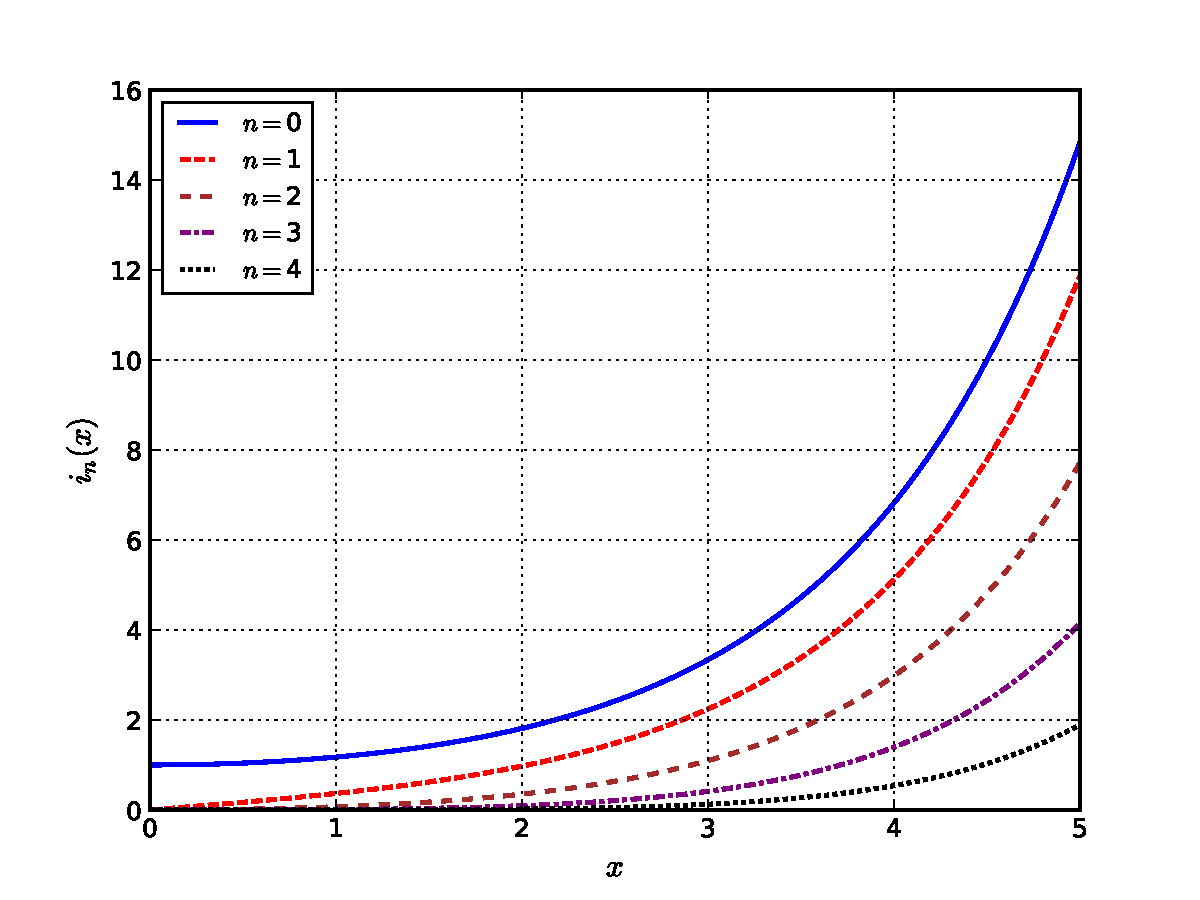
\includegraphics[angle=0,width=0.7\textwidth]{figs/fig-Bessel-Esferica-i.pdf}
\caption{Primeras cinco funciones esf'ericas modificadas de Bessel de primera especie de orden entero.}
\label{fig-in}
\end{figure}
%
\begin{figure}[H]
\centering
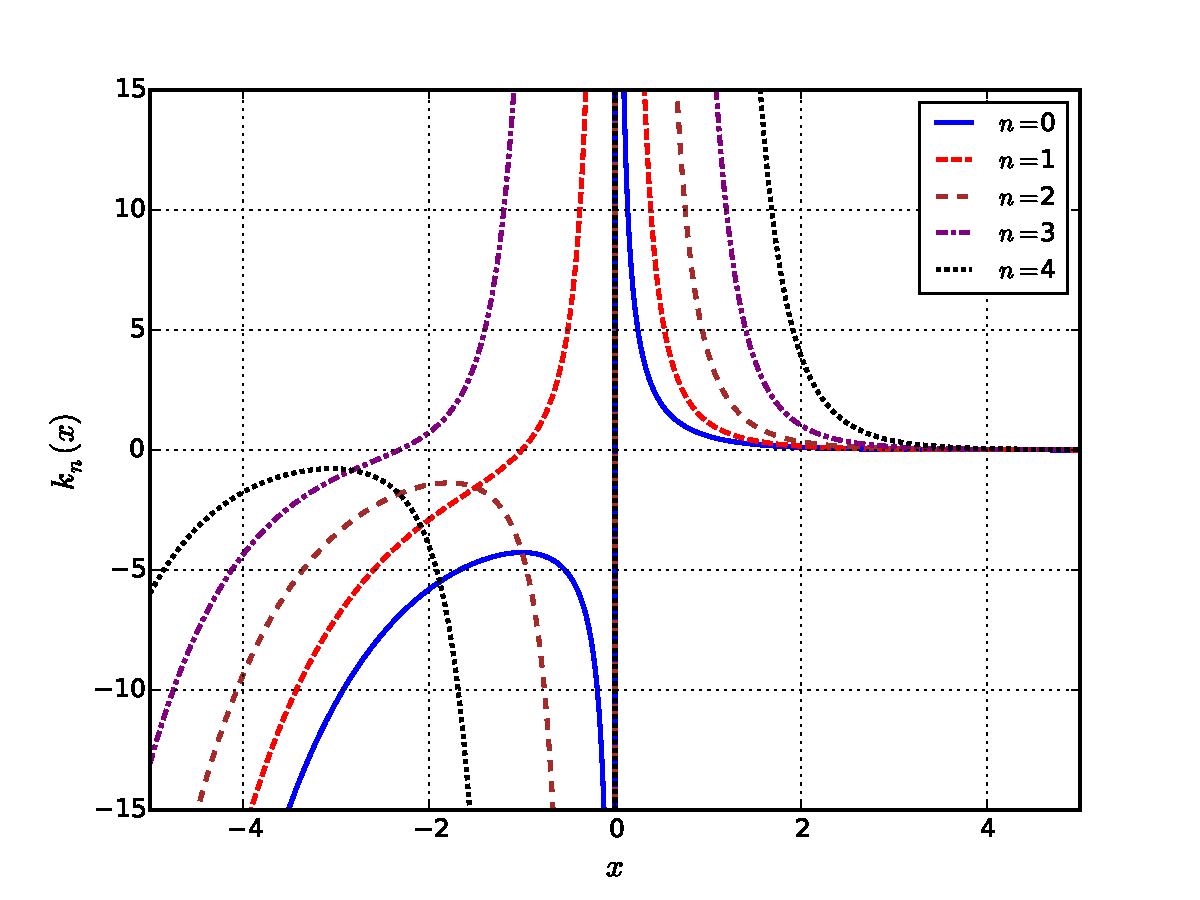
\includegraphics[angle=0,width=0.7\textwidth]{figs/fig-Bessel-Esferica-k.pdf}
\caption{Primeras cinco funciones esf'ericas modificadas de Bessel de segunda especie (funciones de Newmann) de orden entero.}
\label{fig-kn}
\end{figure}
\chapter{Funciones de Green}

\section{Motivaci'on}

El m'etodo de las funciones de Green\footnote{George Green (1793-1841): matem'atico brit'anico. Ver \url{http://es.wikipedia.org/wiki/George_Green}.} permite reducir el problema de encontrar una soluci'on de una \textit{E.D.P. lineal inhomog'enea} a una forma est'andar.

Por ejemplo, en electrost'atica, el potencial satisface la ecuaci'on de Poisson (3D):
\begin{equation}\label{Poisson}
\nabla^2\phi=-\frac{\rho(x)}{\varepsilon_0}.
\end{equation}
Adem'as, sabemos que para una carga puntual ubicada en el punto con coordenadas $\vec{x}'$
\begin{equation}
\phi(\vec{x})=\frac{1}{4\pi\varepsilon_0}\frac{q}{\left|\vec{x}-\vec{x}'\right|},
\end{equation}
y que el potencial producido por una distribuci'on continua de carga con densidad $\rho(\vec{x})$ es
\begin{equation}\label{phirho}
\phi(\vec{x})=\frac{1}{4\pi\varepsilon_0}\int_V\frac{\rho(\vec{x}')}{\left|\vec{x}-\vec{x}'\right|}dV'.
\end{equation}
En ambos casos se eligi'o el potencial nulo en el infinito. Vemos entonces que en la soluci'on general \eqref{phirho} aparece la funci'on
\begin{equation}\label{G1}
G(\vec{x},\vec{x}')=-\frac{1}{4\pi}\frac{1}{\left|\vec{x}-\vec{x}'\right|}.
\end{equation}
de modo que 
\begin{equation}\label{phirho2}
\phi(\vec{x})=\int_V G(\vec{x},\vec{x}')\left(-\frac{\rho(\vec{x}')}{\varepsilon_0}\right)dV'.
\end{equation}
La funci'on \eqref{G1} satisface
\begin{equation}\label{propG1}
\nabla^2G(\vec{x}',\vec{x})=\delta^{(3)}(\vec{x}-\vec{x}').
\end{equation}
Como veremos a continuaci'on, la propiedad \eqref{propG1} es la que permite encontrar soluciones de la ecuaci'on inhomog'enea \eqref{Poisson}.
\begin{align}
\nabla^2\phi(\vec{x}) &= \nabla^2\int_V G(\vec{x},\vec{x}')\left(-\frac{\rho(\vec{x}')} {\varepsilon_0}\right)dV'\\
&= \int_V \left[\nabla^2G(\vec{x},\vec{x}')\right]\left(-\frac{\rho(\vec{x}')}{\varepsilon_0}\right)dV' \\
&= \int_V \delta(\vec{x}-\vec{x}')\left(-\frac{\rho(\vec{x}')}{\varepsilon_0}\right)dV'\\
&= -\frac{\rho(\vec{x})}{\varepsilon_0}.
\end{align}


\section{Generalizaci'on}
Consideremos la E.D.P. lineal inhomog'enea de la forma (en $d$-dimensiones)
\begin{equation}\label{EDP1}
\hat{L}\Psi=f(\vec{x}),
\end{equation}
donde $f(\vec{x})$ es una funci'on ``fuente'' conocida, y $\hat{L}$ es el operador lineal definido por
\begin{equation}
\hat{L}\Psi=\vec\nabla\cdot\left[p(\vec{x})\vec\nabla\Psi\right]+q(\vec{x})\Psi,
\end{equation}
y $p(\vec{x})$ y $q(\vec{x})$ son funciones conocidas.

Para solucionar la E.D.P. \eqref{EDP1} buscamos primero la funci'on de Green $G(\vec{x},\vec{x}')$ asociada al operador $\hat L$, definida como la funci'on que satisface
\begin{equation}\label{EDPG}
\hat{L}G(\vec{x}',\vec{x})=\delta(\vec{x}-\vec{x}').
\end{equation}
La utilidad de introducir la funci'on de Green es que, conociendo una soluci'on de \eqref{EDP1}, es posible escribir la soluci'on del problema inhomog'eneo general \eqref{EDP1} como
\begin{equation}\label{solLG}
\boxed{\Psi(\vec{x})=\int_VG(\vec{x},\vec{x}')f(\vec{x}')dV'+\oint_{\partial V}p(\vec{x}')\left[\Psi(\vec{x}')\vec\nabla' G(\vec{x},\vec{x}')
-G(\vec{x},\vec{x}')\vec\nabla'\Psi(\vec{x}')\right]\cdot d\vec{S}'.}
\end{equation}
Aqu'i $V$ denota el dominio en el que la soluci'on $\Psi$ es v'alida (es decir, $\vec{x}\in V$) y  $\partial V$ su frontera.

Para probar \eqref{solLG} partimos desde la integral sobre $\partial V$ en el en lado derecho de \eqref{solLG}, que luego podemos escribir como una integral de volumen, por medio del teorema de Gauss:
\begin{align}
I &= \oint_{\partial V}p(\vec{x}')\left[\Psi(\vec{x}')\vec\nabla'G(\vec{x},\vec{x}')
-G(\vec{x},\vec{x}')\vec\nabla'\Psi(\vec{x}')\right]\cdot d\vec{S}' \label{I1}\\
&= \int_V\vec\nabla'\cdot\left[p(\vec{x}')\Psi(\vec{x}')\vec\nabla'G(\vec{x},\vec{x}')
-p(\vec{x}')G(\vec{x},\vec{x}')\vec\nabla'\Psi(\vec{x}')\right]dV' \\
&= \int_V\left[\Psi(\vec{x}')\vec\nabla'\cdot\left(p(\vec{x}')\vec\nabla' G(\vec{x},\vec{x}')\right) 
-G(\vec{x},\vec{x}')\vec\nabla'\cdot\left(p(\vec{x}')\vec\nabla'\Psi(\vec{x}')\right)\right]dV' \\
&= \int_V\left[\Psi(\vec{x}')\left(\hat{L}'G(\vec{x},\vec{x}')\right) 
-G(\vec{x},\vec{x}')\left(\hat{L}'\Psi(\vec{x}')\right)\right]dV' \\
&= \int_V\left[\Psi(\vec{x}')\delta(\vec{x}-\vec{x}')
-G(\vec{x},\vec{x}')f(\vec{x}')\right]dV' \\
&= \Psi(\vec{x})- \int_VG(\vec{x},\vec{x}')f(\vec{x}')dV'. \label{I2}
\end{align}
En el 'ultimo paso, hemos asumido que el punto $\vec{x}\in V$  para evaluar la integral que involucra la delta de Dirac. El resultado \eqref{solLG} se sigue de igualar \eqref{I1} y \eqref{I2}.

La soluci'on de la ecuaci'on \eqref{EDPG} queda determinada, adem'as de la funci'on fuente $f(\vec{x})$, por las condiciones de borde del problema. T'ipicamente, estas condiciones de borde se expresan como condiciones que la soluci'on debe satisfacer en la frontera $\partial V$. Esta informaci'on modifica la soluci'on a trav'es de los t'erminos de borde en \eqref{solLG}. Sin embargo, la integral sobre $\partial V$ en \eqref{solLG} depende tanto del valor de la inc'ognita como de su derivada normal, y usualmente no se conoce simult'aneamente estos dos valores. M'as a'un, en general puede ser inconsistente imponer simult'aneamente el valor de $\Psi$ y de su derivada normal en $\partial V$.

\begin{itemize}
\item Si las condiciones de Borde son tipo Dirichlet, es decir, la funci'on $\Psi$ es conocida en $\partial V$, entonces el primer t'ermino en la integral sobre $\partial V$ en \eqref{solLG} es queda determinado luego de encontrar la funci'on de Green, no as'i el segundo t'ermino. Por esta raz'on, en estos casos es \textit{conveniente} elegir una funci'on de Green que satisfaga condiciones de borde tipo Dirichlet homog'eneas en $\partial V$, es decir
\begin{equation}
G(\vec{x},\vec{x}')=0, \qquad \forall\ \vec{x}'\in\partial V.
\end{equation}
Entonces la soluci'on se reduce a
\begin{align}
\Psi(\vec{x}) &= \int_VG(\vec{x},\vec{x}')f(\vec{x}')dV'+\oint_{\partial V}p(\vec{x}')\Psi(\vec{x}')\vec\nabla' G(\vec{x},\vec{x}')\cdot d\vec{S}' \\
&= \int_VG(\vec{x},\vec{x}')f(\vec{x}')dV'+\oint_{\partial V}p(\vec{x}')\Psi(\vec{x}')\frac{\partial G(\vec{x},\vec{x}')}{\partial n'}dS'.
\end{align}

\item Si las condiciones de borde son tipo Neumann, es decir se conoce $\partial\Psi/\partial n=\hat{n}\cdot\vec\nabla\Psi$ sobre $\partial V$, entonces es conveniente escoger una funci'on de Green que satisfaga condiciones de Neumann homog'eneas en la frontera:
\begin{equation}
\frac{\partial G(\vec{x},\vec{x}')}{\partial n'}=0, \qquad \forall\ \vec{x}'\in\partial V.
\end{equation}
Entonces, la soluci'on es dada por
\begin{align}
\Psi(\vec{x}) &= \int_VG(\vec{x},\vec{x}')f(\vec{x}')dV'-\oint_{\partial V}p(\vec{x}')G(\vec{x},\vec{x}')\vec\nabla'\Psi(\vec{x}')\cdot d\vec{S}' \\
&= \int_VG(\vec{x},\vec{x}')f(\vec{x}')dV'-\oint_{\partial V}p(\vec{x}')G(\vec{x},\vec{x}')\frac{\partial \Psi(\vec{x}')}{\partial n'}dS'.
\end{align}
\end{itemize}

Note que, sin embargo, dependiendo del operador $\hat{L}$ puede no ser posible elegir la funci'on de Green tal que $\hat{n}\cdot\vec\nabla'G(\vec{x},\vec{x}')=0$ sobre toda la frontera $\partial V$. Esto ocurre, en el importante caso del operador Laplaciano, $\hat{L}=\nabla^2$.

\section{Simetr'ia de la funci'on de Green}
En el caso particular en el que el operador $\hat{L}$ es el operador Laplaciano, vemos que la  funci'on de Green \eqref{G1} es sim'etrica bajo intercambio de argumentos, es decir, $G(\vec{x},\vec{x}')=G(\vec{x}',\vec{x})$. Puede verificarse que esta propiedad puede implementarse en casos m'as generales, siempre que se satisfagan ciertas condiciones de contorno. Para ver esto, usamos el resultado general \eqref{solLG} en el caso particular en que elegimos $\Psi(\vec{x})=G(\vec{x}'',\vec{x})$, con $\vec{x}'\in V$, y entonces $f(\vec{x})=\delta(\vec{x}''-\vec{x})$. En este caso, encontramos que
\begin{align}\label{simG}
G(\vec{x}'',\vec{x}) &= \int_VG(\vec{x},\vec{x}')\delta(\vec{x}''-\vec{x}')dV' \nonumber\\
& \qquad +\oint_{\partial V}p(\vec{x}')\left[G(\vec{x}'',\vec{x}')\vec\nabla' G(\vec{x},\vec{x}') -G(\vec{x},\vec{x}')\vec\nabla'G(\vec{x}'',\vec{x}')\right]\cdot d\vec{S}' \\
&= G(\vec{x},\vec{x}'')+\oint_{\partial V}p(\vec{x}')\left[G(\vec{x}'',\vec{x}')\vec\nabla' G(\vec{x},\vec{x}')-G(\vec{x},\vec{x}')\vec\nabla'G(\vec{x}'',\vec{x}')\right]\cdot d\vec{S}'. \label{simG2}
\end{align}
Por lo tanto, la funci'on de Green es sim'etrica si la integral del segundo t'ermino en \eqref{simG2} se anula. Esto puede ocurrir, t'ipicamente, si la funci'on de Green se anula en la frontera:
\begin{equation}
G(\vec{x},\vec{x}')=0, \qquad \forall\ \vec{x}'\in\partial V
\end{equation}

\section{Expresiones expl'icitas de algunas funciones de Green}
La funci'on de Green definida por la ecuaci'on \eqref{EDPG} no es 'unica. Si $G_1(\vec{x},\vec{x}')$ es soluci'on, entonces $G_2(\vec{x},\vec{x}'):=G_1(\vec{x},\vec{x}')+H(\vec{x},\vec{x}')$ tambi'en es soluci'on, si $H(\vec{x},\vec{x}')$ es soluci'on del problema homog'eneo asociado, 
\begin{equation}
\hat{L}H(\vec{x},\vec{x}')=0.
\end{equation}
Este hecho permite considerar soluciones soluciones particulares simples como base para otras funciones de Green, que pueden obtenerse agregando una soluci'on de la ecuaci'on homog'enea de modo que la funci'on resultante satisfaga las condiciones de borde que simplifiquen el problema.

\subsection{Operador Laplaciano}
En este caso $p(\vec{x})=1$ y $q(\vec{x})=0$. En F'isica, usualmente se busca la funci'on de Green que ``respete la homogeneidad e isotrop'ia del espacio''. La primera condici'on (homogeneidad) significa que $G$ funci'on que depende de $\vec{x}$ y $\vec{x}'$ s'olo a trav'es de su diferencia $\vec{x}-\vec{x}'$. La segunda condici'on (isotrop'ia=invariancia bajo rotaciones) implica que $G$ s'olo depende del m'odulo de $\vec{x}-\vec{x}'$. Esto reduce la funci'on de Green b'asicamente a una funci'on de una variable, ya que entonces
\begin{equation}
G(\vec{x},\vec{x}')=G(|\vec{x}-\vec{x}'|).
\end{equation}

\subsubsection{$D=3$}
En coordenadas esf'ericas centradas en $\vec{x}'$
\begin{equation}\label{n2Gd}
\nabla^2G=\frac{1}{r^2}\frac{d\ }{dr}\left(r^2\frac{dG}{dr}\right)=\delta^{(3)}(r)
\end{equation}
por lo tanto 
\begin{equation}
\frac{1}{r^2}\frac{d\ }{dr}\left(r^2\frac{dG}{dr}\right)=0, \qquad r\neq 0.
\end{equation}
La soluci'on para $r\neq 0$ se encuentra entonces r'apidamente integrando esta ecuaci'on, obteniendo
\begin{equation}
G(r)=\alpha+\frac{\beta}{r}.
\end{equation}
Por otro lado, la condici'on \eqref{n2Gd} implica, usando el teorema de Gauss, que
\begin{equation}
\int_{\partial V}\vec\nabla G\cdot d\vec{S}=\int_{\partial V}\frac{dG}{dr}r^2d\Omega=1,
\end{equation}
que requiere entonces que $-4\pi\beta=1$. Finalmente, en la mayor'ia de los problemas es conveniente elegir una funci'on de Green que se anule para distancias muy grandes, es decir, tal que $\lim_{r\to\infty}G(r)=0$. Esta condici'on impone que $\alpha=0$ (note que, equivalentemente, esta condici'on implica agregar la soluci'on homog'enea $H=-\alpha$ a la funci'on de Green original), y por lo tanto
\begin{equation}
\boxed{G(\vec{x}-\vec{x}')=-\frac{1}{4\pi}\frac{1}{|\vec{x}-\vec{x}'|}.}
\end{equation}

\subsubsection{$D=2$}
En coordenadas polares $(\rho,\varphi)$ centradas en $\vec{x}'$, con $G=G(\rho)$
\begin{equation}
\nabla^2G=\frac{1}{\rho}\frac{d\ }{d\rho}\left(\rho\frac{dG}{d\rho}\right)=\delta^{(2)}(\rho).
\end{equation}
Integrando la ecuaci'on para $\rho\neq 0$, es decir,
\begin{equation}
\frac{1}{\rho}\frac{d\ }{d\rho}\left(\rho\frac{dG}{d\rho}\right)=0,
\end{equation}
encontramos que
\begin{equation}
G(\rho)=\alpha+\beta\ln\rho.
\end{equation}
Nuevamente, el teorema de Gauss (versi'on 2D), 
\begin{equation}
\int_{\partial S}\vec\nabla G\cdot d\vec{S}=\oint\frac{dG}{d\rho}\rho\,d\varphi=2\pi\beta=1.
\end{equation}
De esto modo, eliminando el t'ermino constante (que es una soluci'on de la ecuaci'on homog'enea), encontramos
\begin{equation}
\boxed{G(\vec{x}-\vec{x}')=\frac{1}{2\pi}\ln{|\vec{x}-\vec{x}'|}.}
\end{equation}

%\subsubsection{$D=1$}
%En este caso, usando una coordenada cartesiana centrada en $x'$, tenemos
%\begin{equation}\label{n2Gd1}
%\nabla^2G(|x|)=\frac{d^2G(|x|)}{dx^2}=\delta(x),
%\end{equation}
%y por lo tanto
%\begin{equation}
%\frac{d^2G}{dx^2}=0, \qquad x\neq 0.
%\end{equation}
%Integrando esta condici'on para $x>0$ encontramos que
%\begin{equation}
%G(x)=\alpha+\beta x, \qquad x>0,
%\end{equation}
%y entonces
%\begin{equation}
%G(|x|)=\alpha+\beta |x|, \qquad x\neq 0.
%\end{equation}
%Integrando \eqref{n2Gd1} en el intervalo $[-a,a]$, $a>0$ y usando el teorema fundamental del c'alculo (``Teorema de Gauss 1D''), encontramos
%\begin{equation}
%\int_{-a}^a\frac{d^2G}{dx^2}=\left.\frac{dG}{dx}\right|^a_{-a}=\beta-(-\beta)=2\beta=1.
%\end{equation}
%Vemos que en este caso
%\begin{equation}
%G(x,x')=\alpha+\frac{1}{2}|x-x'|,
%\end{equation}
%de donde vemos que no existe una fuci'on de Green que satisfaga $G\to 0$ para $|x-x'|\to\infty$.

\subsection{Operador de Helmoltz}
En el caso del operador de Helmholtz $\hat{L}=\nabla^2+k^2$, que corresponde al caso $p(\vec{x})=1$ y $q(\vec{x})=k^2$.

En cada caso, buscaremos las funciones de Green de la forma $G(\vec{x},\vec{x}')=G(|\vec{x}-\vec{x}'|)$

\subsubsection{$D=3$}
En coordenadas esf'ericas centradas en $\vec{x}'$
\begin{equation}\label{HGd}
(\nabla^2+k^2)G=\frac{1}{r^2}\frac{d\ }{dr}\left(r^2\frac{dG}{dr}\right)+k^2G=\delta^{(3)}(r),
\end{equation}
por lo tanto 
\begin{equation}\label{HG0}
\frac{1}{r^2}\frac{d\ }{dr}\left(r^2\frac{dG}{dr}\right)+k^2G=0, \qquad r\neq 0.
\end{equation}
Para solucionar \eqref{HG0} realizamos el cambio de variable $G(r)=u(r)/r$, que conduce a $r^2dG/dr=ru'-u$. Con esto, \eqref{HG0} se reduce a $u''+k^2u=0$. Por lo tanto, las soluciones son de la forma
\begin{equation}\label{GH3d}
G(r)=\alpha\frac{e^{ikr}}{r}+\beta\frac{e^{-ikr}}{r}.
\end{equation}
Con esta soluci'on, v'alida para $r\neq 0$, retornamos a la ecuaci'on \eqref{HGd} que, luego de integrar sobre una esfera de radi $R$ centrada en $r=0$ y usando el teorema de Gauss, implica que
\begin{align}
1 &= \oint_{\partial V}\vec\nabla G\cdot d\vec{S}+k^2\int_VG\,dV \\
&= \oint_{\partial V}\frac{dG}{dr}r^2d\Omega+k^2\int_VGr^2\,drd\Omega \\
&= 4\pi G'R^2+4\pi k^2\int_0^R Gr^2\,dr \\
&= 4\pi\left[\alpha\left(ikR-1\right)e^{ikR}-\beta\left(ikR+1\right)e^{-ikR}\right]+4\pi k^2\int_0^R \left[\alpha e^{ikr}+\beta e^{-ikr}\right]r\,dr \\
&= -4\pi(\alpha+\beta).
\end{align}
De esta forma encontramos las condici'on
\begin{equation}
\alpha+\beta=-\frac{1}{4\pi},
\end{equation}
que permite escribir la soluci'on \eqref{GH3d} como
\begin{equation}\label{GH3d2}
G(r)=-\frac{1}{4\pi}\frac{e^{ikr}}{r}-i\beta\frac{\sen(kr)}{r}.
\end{equation}
Note que el segundo t'ermino es una soluci'on de la ecuaci'on de Helmholtz \textit{homog'nenea} (es proporcional a la funci'on esf'erica de Bessel $j_0(kr)$). Por lo tanto, es posible elegir
\begin{equation}\label{GH3d3}
\boxed{G^{+}(\vec{x},\vec{x}')=-\frac{1}{4\pi}\frac{e^{ik|\vec{x}-\vec{x}'|}}{|\vec{x}-\vec{x}'|},}
\end{equation}
que corresponde a la elecci'on $\beta=0$. An'alogamente, podeomos considerar la funci'on de Green 
\begin{equation}\label{GH3d4}
G^{-}(\vec{x},\vec{x}')=-\frac{1}{4\pi}\frac{e^{-ik|\vec{x}-\vec{x}'|}}{|\vec{x}-\vec{x}'|},
\end{equation}
que se encuentra en el caso en que $\beta=-1/4\pi$.

\subsubsection{$D=2$}
En coordenadas polares $(\rho,\varphi)$ centradas en $\vec{x}'$, con $G=G(\rho)$
\begin{equation}\label{HGd2d}
(\nabla^2+k^2)G=\frac{1}{\rho}\frac{d\ }{d\rho}\left(\rho\frac{dG}{d\rho}\right)+k^2G=\delta^{(2)}(\rho).
\end{equation}
Para $\rho\neq 0$, 
\begin{equation}
\frac{1}{\rho}\frac{d\ }{d\rho}\left(\rho\frac{dG}{d\rho}\right)+k^2G=0.
\end{equation}
Definiendo $x:=k\rho$ esta ecuaci'on se reduce a
\begin{equation}
x\frac{d\ }{dx}\left(x\frac{dG}{dx}\right)+x^2G(x)=0, \qquad x\neq 0,
\end{equation}
que es la ecuaci'on de Bessel de orden $\nu=0$, ver \eqref{Besselec1}. Por lo tanto, su soluci'on general es de la forma
\begin{equation}
G(\rho)=\alpha J_0(k\rho)+\beta N_0(k\rho)=\tilde\alpha H^{(1)}_0(k\rho)+\tilde\beta H^{(2)}_0(k\rho).
\end{equation}
Nuevamente, retornando a la ecuaci'on original \eqref{HGd2d} e integrando sobre un c'irculo $S$ de radio $R$ centrado en $\rho=0$, obtenemos
\begin{align}
1 &= \oint_{\partial S}\vec\nabla G\cdot d\vec{S}+k^2\int_S G\,dS \\
&= 2\pi\left[R\frac{dG}{d\rho}(kR)+k^2\int_0^RG\rho\,d\rho\right] \\
&= 2\pi\left[kR\left(\tilde\alpha H'^{(1)}_0(kR)+\tilde\beta H'^{(2)}_0(kR)\right)+\int_0^{kR}\left(\tilde\alpha H^{(1)}_0(x)+\tilde\beta H^{(2)}_0(x)\right)x\,dx\right].
\end{align}
Usando las identidades $H'^{(1)}_0(x)=-H_1^{(1)}(x)$ y $xH_0^{(1)}(x)=d[xH_1^{(1)}(x)]/dx$ y similarmente para $H'^{(2)}_0$ y $H'^{(2)}_1$, evaluamos la expresi'on anterior, obteniendo
\begin{align}
1 &= -2\pi\lim_{x\to 0}\left(\tilde\alpha xH_1^{(1)}(x)-\tilde\beta xH_1^{(2)}(x)\right) \\
&= 2\pi\left[\tilde\alpha\frac{2i}{\pi} -\tilde\beta\frac{2i}{\pi} \right]\\ 
&= 4i(\tilde\alpha -\tilde\beta).
\end{align}
Con esto, la soluci'on adopta la forma
\begin{align}
G(\rho) &= -\frac{i}{4}H_0^{(1)}(k\rho)+\tilde\beta\left(H_0^{(1)}(k\rho)+H_0^{(2)}(k\rho)\right)\\
&= -\frac{i}{4}H_0^{(1)}(k\rho)+2\tilde\beta J_0(k\rho).
\end{align} 
Tal como en el caso anterior, el t'ermino proporcional a $\tilde\beta$ es una soluci'on del problema homog'eneo. Si elegimos $\tilde\beta=0$, encontramos la siguiente funci'on de Green:
\begin{equation}
\boxed{G^{(1)}(\vec{x},\vec{x}') = -\frac{i}{4}H_0^{(1)}(k|\vec{x}-\vec{x}'|).}
\end{equation}
Alternativamente, si se elige $\tilde\alpha=0$, se encuentra
\begin{equation}
G^{(2)}(\vec{x},\vec{x}') = \frac{i}{4}H_0^{(2)}(k|\vec{x}-\vec{x}'|).
\end{equation}
\chapter{Tensores}
\section{Tensores Cartesianos}

En muchas 'areas de la F'isica es 'util, y frecuentemente necesario, definir \textit{objetos con m'ultiples componentes} respecto a un sistema de coordenadas (SC). En general, los valores de las componentes de estos objetos cambian al ser calculados respecto de otro SC. En particular, es posible \textit{clasificar} este tipo de objetos de acuerdo a c'omo cambian sus componentes bajo una transformaci'on de coordenadas (TC). Esta clasificaci'on permite en particular definir \textbf{tensores} como conjunto de cantidades (las ``componentes del tensor") tales que su relaci'on al cambiar de SC es sencilla (en particular, lineal y homog'enea). En este tipo de an'alisis es importante recordar que \textit{la definici'on de vectores y tensores depende del tipo de transformaci'on} (en general, de coordenadas) bajo consideraci'on. Esto se debe a que, \textit{algunas cantidades pueden formar tensores respecto a un tipo de transformaci'on, pero no serlo respecto a otro tipo de transformaciones}. En otras palabras, la definici'on de tensores es relativa a la transformaci'on considerada. En distintos contextos y teor'ias f'isicas es conveniente considerar transformaciones de distinto tipo (que en general est'an relacionadas con la invariancia de las leyes f'isicas respectivas bajo ese tipo de transformaci'on). Por ejemplo, en mec'anica de Newton (y en general, en teor'ias no-relativistas) es conveniente asegurar que las leyes f'isicas consideradas sean v'alidas independientemente de la orientaci'on de los ejes cartesianos elegidos para un determinado c'alculo. En otras palabras, es necesario considerar c'omo cambian las diversas cantidades bajo \textbf{rotaciones}. Para esto, es 'util definir cantidades que sean vectores y tensores respecto a transformaciones ortogonales de coordenadas (TOC, es decir, rotaciones). Por otro lado, en la teor'ia de Relatividad Especial se considera que $(ct,x,y,z)$ son las cuatro coordenadas asociadas a un evento dado, respecto a un Sistema de Referencia Inercial (SRI). Las transformaciones de las coordenadas del mismo evento entre dos SRI's son en ese caso las \textbf{transformaciones de Lorentz}, que pueden expresarse como una transformaci'on lineal de las coordenadas $(ct,x,y,z)$. En este contexto es 'util entonces considerar (definir) cantidades que transformen como ``cuadri"-tensores bajo transformaciones de Lorentz. Note, sin embargo, que un vector respecto a TOC no define necesariamente un vector bajo transformaciones de Lorentz. 

Analizaremos primero la definici'on, las propiedades b'asicas y la utilidad pr'actica de los tensores respecto a TOC.

\section{Bases ortogonales}

Considere un espacio Euclideano $n$-dimensional ($E_n$), donde cada punto de $E_n$ tiene coordenadas $x_i$, $i=1,\cdots, n$, con respecto a un \textbf{sistema ortogonal de coordenadas} (SOC) $K$. 

Consideramos una \textbf{base ortonormal} (BON) $\lbrace\hat{e}_i\rbrace$ ($i=1,\cdots, n$) de vectores, es decir, tal que
\begin{equation}
\boxed{\hat{e}_i\cdot \hat{e}_j=\delta_{ij},}
\end{equation}
donde $\delta_{ij}$ denota la \textbf{Delta de Kronecker}, definida como los $n^2$ valores dados por
\begin{equation} \label{DK}
\delta_{ij}:=\begin{cases} 1, & \text{si } i=j \\ 0, & \text{si } i\neq j\end{cases} .
\end{equation}
Note que esta Delta de Kronecker puede ser representada matricialmente por la matriz identidad $n\times n$. 

En el espacio euclideano $E_n$ es posible definir (consistentemente) el \textbf{vector posici'on} $\vec{x}$, que une el origen del SCO con un punto con coordenadas $x_i$, por
\begin{equation}
\vec{x}=\sum_{i=1}^n x_i\hat{e}_i.
\end{equation}
En este sentido, las coordenadas $x_i$ son componentes del vector $\vec{x}$ en la base $\lbrace\hat{e}_i\rbrace$, y pueden expresarse como
\begin{equation}\label{x2}
x_i=\vec{x}\cdot\hat{e}_i.
\end{equation}

En general, la BON $\lbrace\hat{e}_i\rbrace$ permite descomponer cada vector $\vec{A}$ en sus respectivas componentes:
\begin{equation}\label{V1}
\vec{V}=\sum_{i=1}^nv_i\hat{e}_i,
\end{equation}
donde
\begin{equation}\label{v2}
v_i=\vec{V}\cdot\hat{e}_i.
\end{equation}


\section{Transformaciones ortogonales}
\begin{figure}[H]
\centering
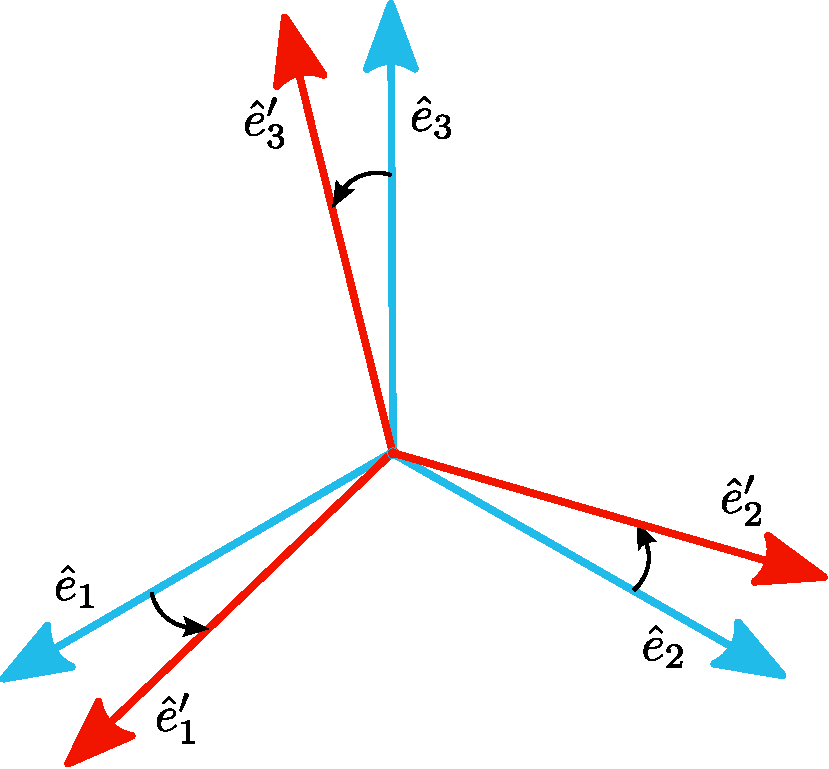
\includegraphics[angle=0,width=0.3\textwidth]{figs/fig-rotacion-bases.pdf}
\caption{Una transformaci'on ortogonal (rotaci'on) de bases ortonormales.}
\label{fig-rotacion}
\end{figure}
Consideremos ahora un nuevo SOC $x'_i$ relacionado con el SOC $x_i$ por medio de una \textbf{transformaci'on ortogonal (TO) de coordenadas}, es decir, una \textbf{rotaci'on}, ver figura \ref{fig-rotacion}.


Esta transformaci'on induce una nueva BON $\lbrace\hat{e}'_i\rbrace$. Respecto a esta nueva base, un vector $\vec{V}$ tiene componentes $\vec{v}_i$ tales que
\begin{equation}\label{V2}
\vec{V}=\sum_{i=1}^nv'_i\hat{e}'_i.
\end{equation}

Es posible relacionar las bases $\lbrace\hat{e}_i\rbrace$  y $\lbrace\hat{e}'_i\rbrace$ ya que cada vector $\hat{e}'_i$ puede escribirse como una combinaci'on lineal de los vectores base $\hat{e}_i$, esto es, existe una relaci'on de la forma
\begin{equation}\label{epe0}
\hat{e}'_i=\sum_{j=1}^n a_{ij}\hat{e}_j.
\end{equation}

La condici'on que la transformaci'on \eqref{epe0} sea efectivamente una TO, es decir, que transforme una BON en una nueva BON impone ($n(n+1)/2$) condiciones sobres los ($n^2$) coeficientes (la ``matriz'') de transformaci'on $a_{ij}$. En efecto,
\begin{align}
\delta_{ij} &= \hat{e}'_i\cdot \hat{e}'_j \\
&= \left(\sum_{k=1}^na_{ik}\hat{e}_k\right)\cdot \left(\sum_{l=1}^na_{jl}\hat{e}_l\right) \\
&=\sum_{k=1}^n\sum_{l=1}^n a_{ik}a_{jl}\left(\hat{e}_k\cdot \hat{e}_l\right) \\
&= \sum_{k=1}^n\sum_{l=1}^na_{ik}a_{jl}\,\delta_{kl} \\
&= \sum_{k=1}^na_{ik}a_{jk}, 
\end{align}
y por lo tanto,
\begin{equation}\label{aad1}
\boxed{\sum_{k=1}^n a_{ik}a_{jk}=\delta_{ij}.}
\end{equation}
En \textbf{notaci'on matricial}, 
\begin{equation} \label{aat1}
\mathbb{A}\cdot(\mathbb{A}^\top)=\mathbb{I}.
\end{equation}
Al calcular el determinante de (\ref{aat1}) encontramos que
\begin{equation}
(\det\mathbb{A})^2=1,
\end{equation}
por lo que necesariamente $\det\mathbb{A}=1$ o bien $\det\mathbb{A}=-1$. Si $\det\mathbb{A}=1$ decimos que la TO es una \textbf{transformaci'on propia}, mientras que si $\det\mathbb{A}=-1$ ella es \textbf{impropia}. En todo caso $\det\mathbb{A}\neq 0$, de modo que la inversa $\mathbb{A}^{-1}$ siempre existe y es 'unica. De  (\ref{aat1}) vemos entonces que la matriz inversa de una transformaci'on ortogonal coincide con su transpuesta,
\begin{equation}\label{corto}
\mathbb{A}^{-1}=\mathbb{A}^\top ,
\end{equation}
y por lo tanto se satisface adem'as que
\begin{equation} \label{ata1}
(\mathbb{A}^\top)\cdot\mathbb{A}=\mathbb{I},
\end{equation}
o, en notaci'on de 'indices,
\begin{equation}\label{aakd2}
\boxed{\sum_{k=1}^n a_{ki}a_{kj}=\delta_{ij}.}
\end{equation}

Puede verificarse a partir de estas propiedades b'asicas que el conjunto de \textit{todas} las transformaciones ortogonales en un espacio Euclideano $n$-dimensional forman un \textbf{grupo}\footnote{Ver, por ejemplo, \url{http://es.wikipedia.org/wiki/Grupo_(matematica)}.}: el grupo ortogonal\footnote{Ver, por ejemplo, \url{http://es.wikipedia.org/wiki/Grupo_ortogonal}.} $n$-dimensional, $O(n)$.

Usando \eqref{x2} y \eqref{epe0} podemos relacionar las coordenadas $x_i$ (asociadas a un mismo vector posici'on $\vec{x}$) en respecto a los dos SOC:
\begin{equation}
\boxed{x'_i=\sum_{j=1}^na_{ij}x_j,} \label{xpax0}
\end{equation}


\section{Convenci'on de suma de Einstein}

Es conveniente introducir la \textbf{convenci'on de suma de Einstein}, que establece que \textit{en toda expresi'on donde se repitan dos 'indices iguales, se subentiende que existe una suma sobre todo el rango de variaci'on del 'indice}.  De esta forma, (\ref{V1}), (\ref{V2}),  (\ref{epe0}), \eqref{aad1}, \eqref{aad1} y \eqref{x2} pueden abreviarse de la forma siguiente,
\begin{equation}\label{V1b}
\vec{V}=v_i\hat{e}_i,
\end{equation}
\begin{equation}\label{V2b}
\vec{V}=v'_i\hat{e}'_i,
\end{equation}
\begin{equation}\label{epe}
\hat{e}'_i= a_{ij}\hat{e}_j,
\end{equation}
\begin{equation}\label{aatdel}
a_{ik}a_{jk}=\delta_{ij},
\end{equation}
\begin{equation}
a_{ki}a_{kj}=\delta_{ij},
\end{equation}
\begin{equation}\label{xpax}
x'_i=a_{ij}x_j.
\end{equation}

\section{Vectores}
Como vimos, un vector $\vec{V}$ puede ser descompuesto tanto en una base ortonormal $K$ como en otra $K'$. A partir de esto, podemos encontrar la forma en que est'an relacionadas las componentes de $\vec{V}$ respecto a dos SOC's. Usando \eqref{v2} y \eqref{epe} encontramos, an'alogamente a \eqref{xpax} que
\begin{equation}
v'_i=a_{ij}v_j.
\end{equation}
Esta propiedad puede ser considerada como la \textit{definici'on} de (las componentes de) un vector: 
\begin{quotation}
\textbf{Definici'on:} Diremos que el conjunto de $n$ n'umeros $\lbrace v_1, v_2,\cdots, v_n\rbrace$, definidos en cada BO (SOC), son las componentes de un vector (cartesiano) si y s'olo si bajo toda TO's (e.d., definidas por una matriz $\mathbb{A}$ que satisface (\ref{corto})), sus valores est'an relacionados por 
\begin{equation}\label{dv}
\boxed{v'_i=a_{ij}v_j.}
\end{equation}
\end{quotation}
Note que en un espacio Euclideano las coordenadas $x_i$ de un punto de $E_n$ transforman de acuerdo a \eqref{xpax} bajo TO's y pueden por lo tanto ser consideradas como las componentes de un vector (del ``vector posici'on'' $\vec{x}$)\footnote{El hecho que las coordenadas transformen como componentes de un vector \textit{no es} un resultado general. Al considerar la definici'on de vectores y tensores respecto a transformaciones generales de coordenadas, o en particular bajo transformaciones no-lineales, no es posible considerar las coordenadas de los puntos del espacio como componentes de un vector, simplemente porque su ley de transformaci'on difiere de la ley v'alida para los objetos definidos como vectores. En estos casos se define un vector por la ley de transformaci'on $v'_i=({\partial x'_i}/{\partial x_j})v_j$, que en el caso de transformaciones lineales coincide con (\ref{dv}), ya que ${\partial x'_i}/{\partial x_j}=a_{ij}$.}. 


Otro ejemplo de vector es la velocidad de una part'icula (movi'endose en $E_n$). Si $x_i(t)$ son las coordenadas de la trayectoria de la part'icula en funci'on del tiempo $t$ entonces la velocidad instant'anea transforma como (``es'') un vector bajo TO's. En efecto, la velocidad instant'anea es definida, \textit{en cada SOC}, por $v_i:=dx_i/dt$. Entonces, en un SOC $K'$ relacionado con $K$ por medio de (\ref{xpax}), tendremos que las ``nuevas'' componentes de la velocidad ser'an
\begin{equation}
v'_i:=\frac{dx'_i}{dt}=\frac{d\ }{dt}(a_{ij}x_j)=a_{ij}\frac{dx_j}{dt}=a_{ij}v_j.
\end{equation}
Aqu'i hemos asumido que los coeficientes $a_{ij}$ son independientes del tiempo (constantes). De forma an'aloga, la aceleraci'on es tambi'en un vector bajo TO's.

Note que \textit{no toda colecci'on de $n$-valores definidos en cada SOC pueden considerarse componentes de un vector}. Por ejemplo, la densidad de masa $\rho$ de un cuerpo, su temperatura $T$, y la componente $z$ de su momentum $p_z$, son cantidades que pueden definirse en cada SOC, sin embargo, el conjunto de 3 cantidades $(\rho,T,p_z)$ no forman las componentes de un vector, simplemente porque sus valores no est'an relacionados bajo TO's de la forma (\ref{dv}).

%En general, si un 'indice est'a repetido en una expresi'on, es decir, si hay una suma impl'icita, es irrelevante la elecci'on particular del 'indice repetido (puede ser $i$, $j$, $k$, etc.), el valor de la expresi'on es el mismo independiente de la letra empleada para denotar el 'indice de suma. Por esta raz'on, los indices de suma (es decir, repetidos) son tambi'en llamados \textit{'indices mudos}, siendo posible entonces cambiar a voluntad la letra particular usada.


\section{Escalares}

Un \textbf{escalar} es una cantidad que no cambia su valor al rotar el SOC, es decir, una cantidad que permanece \textit{invariante bajo TO's}. Ejemplos de cantidades escalares en Mec'anica Cl'asica (no-relativista) son: la masa de un cuerpo, el volumen de un cuerpo, el coeficiente de roce entre dos superficies, la temperatura, la energ'ia cin'etica, etc. En t'erminos matem'aticos, si $\phi$ es una cantidad definida en cada SOC, entonces ella es un escalar si y s'olo si
\begin{equation}
\phi'=\phi.
\end{equation}
Otro ejemplo de una cantidad escalar bajo TO's es el producto escalar entre vectores. Si $A_i$ y $B_i$ son las componentes de dos vectores $\vec{A}$ y $\vec{B}$ respectivamente, entonces su producto escalar permanece invariante:
\begin{align}
A'_iB'_i &= (a_{ij}A_j)(a_{ik}B_k) \\
&= (a_{ij}a_{ik})A_jB_k \\
&= \delta_{jk}A_jB_k \\ 
&= A_jB_j \\
&= A_iB_i.
\end{align}


\section{Tensores}
Tanto en Mec'anica, como en Electrodin'amica, es habitual encontrar cantidades \textit{con m'as de un 'indice} (es decir, con m'as de $n$ componentes), del tipo $T_{ij}$, $A_{ijk}$, etc. 

Por ejemplo, en Mec'anica la relaci'on entre el momentum angular de un cuerpo en rotaci'on y su vector velocidad angular involucra el \textbf{tensor momento de inercia} $I_{ij}$. En efecto, considere un cuerpo caracterizado por su densidad $\rho(x_i)$, contenido en una regi'on $V$, \textit{rotando r'igidamente} respecto a un eje caracterizado por la direcci'on $\hat{\omega}$, con velocidad angular $\omega$. Entonces su momentum angular respecto al origen del SOC, \textit{ubicado sobre el eje de rotaci'on}, es dado por
\begin{align}
\vec{L} &= \int_V\vec{x}\times d\vec{p}\\
&= \int_V\rho(x)\vec{x}\times \vec{v}\,dV\\
&= \int_V\rho(x)\vec{x}\times \left(\vec{\omega}\times\vec{x}\right) dV.
\end{align}
Usando la identidad $\vec{A}\times (\vec{B}\times\vec{C})\equiv \vec{B}(\vec{A}\cdot\vec{C})-\vec{C}(\vec{A}\cdot\vec{B})$, podemos escribir
\begin{align}
\vec{L} &= \int_V\rho(x)\left[\vec{\omega}(\vec{x}\cdot\vec{x})-\vec{x}(\vec{\omega}\cdot\vec{x})\right] dV ,
\end{align}
o, en t'erminos de componentes,
\begin{align}
L_i &= \int_V\rho(x)\left[\omega_i(x_kx_k)-x_i(\omega_j x_j)\right]dV  \\
&= \int_V\rho(x)\left[(\delta_{ij}\omega_j)(x_kx_k)-x_i(\omega_j x_j)\right]dV  \\
&= \left(\int_V\rho(x)\left[\delta_{ij}(x_kx_k)-x_i x_j\right]dV \right) \omega_j ,
\end{align}
es decir,
\begin{equation}\label{LIo}
\boxed{L_i=I_{ij}\,\omega_j,}
\end{equation}
con 
\begin{equation}
\boxed{I_{ij}:=\int_V\rho(x)\left[\delta_{ij}(x_kx_k)-x_i x_j\right]dV .}
\end{equation}
Note que este resultado expresa el hecho que, en general, \textit{el momentum angular de un cuerpo en rotaci'on no es necesariamente paralelo al eje de rotaci'on}. Puede encontrar algunos ejemplos de tensores momento de inercia para distintos cuerpos respecto a SOC particulares \href{http://en.wikipedia.org/wiki/List_of_moment_of_inertia_tensors}{aqu\'i}.

Analizemos ahora c'omo cambian las componentes $I_{ij}$ cuando ellas son calculadas en otro SOC. Si analizamos el movimiento respecto a un SOC rotado respecto al primero, de modo que las coordenadas de cada punto son ahora dadas por (\ref{xpax}), entonces tendremos que las componentes $I'_{ij}$ estar'an dadas por
\begin{align}
I'_{ij} &:= \int_V\rho'(x')\left[\delta_{ij}(x'_kx'_k)-x'_i x'_j\right]dV'  \\
&= \int_V\rho(x)\left[\delta_{ij}(x_kx_k)-(a_{il}x_l)(a_{jm}x_m)\right]dV \label{trI1}\\
&= \int_V\rho(x)\left[(a_{il}a_{jl})(x_kx_k)-(a_{il}x_l)(a_{jm}x_m)\right] \label{trI2}\\
&= \int_V\rho(x)\left[(a_{il}a_{jm}\delta_{lm})(x_kx_k)-(a_{il}x_l)(a_{jm}x_m)\right]dV \\
&= a_{il}a_{jm}\int_V\rho(x)\left[\delta_{lm}(x_kx_k)-x_lx_m\right]dV \\
&= a_{il}a_{jm}\,I_{lm}.
\end{align}
Note que aqu'i hemos usado el hecho que la masa se considera un escalar, de modo que $dm=\rho(x)dV=\rho'(x')dV'$. Adem'as, la condici'on \eqref{aatdel} fue usada en para reescribir el primer t'ermino de \eqref{trI1} en la forma que aparece en la expresi'on \eqref{trI2}.

En resumen,
\begin{equation}\label{IpI}
I'_{ij} =a_{il}a_{jm}\,I_{lm}.
\end{equation}

Es simple verificar usando (\ref{IpI}) y el hecho que $\omega_i$ son componentes de un vector que $L_i$, dado por (\ref{LIo}), efectivamente satisface la ley de transformaci'on de un vector.

Vemos que las $n^2$ cantidades\footnote{De las cuales s'olo $n(n+1)/2$ son linealmente independientes, debido a que $I_{ij}=I_{ji}$.} $I_{ij}$ cambian los valores de sus componentes al ser calculadas en distintos SOC, pero estos valores est'an relacionados de una forma (relativamente) simple. Las cantidades cuyas componentes transforman de la forma (\ref{IpI}) son llamadas \textbf{tensores de rango 2}\footnote{Otros ejemplos de tensores de rango 2 'utiles en F'isica son: el tensor diel'ectrico de un medio polarizable $\kappa_{ij}$, el tensor de tensiones de un fluido $t_{ij}$, el tensor de conductividad de un material conductor $\sigma_{ij}$, el tensor de deformaci'on de un medio el'astico $\varepsilon_{ij}:=(\partial_i u_j+\partial_j u_i)/2$ ($u_i$ es el vector desplazamiento).}.

\begin{quotation}
\textbf{Definici'on:} Diremos que el conjunto de $n^2$ cantidades $T_{ij}$ ($i,j=1,\dots, n$) definidas en cada SOC, son las componentes de un \textbf{tensor cartesiano de rango 2} si y s'olo si, bajo cada TO (de la forma \eqref{xpax}, con la condici'on \eqref{aatdel}) sus valores est'an relacionados por\footnote{En notaci'on matricial, $\mathbb{T}'=\mathbb{A}\mathbb{T}\mathbb{A}^T$.} 
\end{quotation}
\begin{equation}\label{dT2}
\boxed{T'_{ij}=a_{ik}a_{jl}\,T_{kl}.}
\end{equation}
Note que la relaci'on inversa es dada por
\begin{equation}
T_{ij}=a_{ki}a_{lj}T'_{kl}.
\end{equation}

Similarmente al caso del momentum angular, podemos analizar la \textbf{energ'ia cin'etica} del cuerpo rotando r'igidamente,
\begin{align}
K &=\frac{1}{2}\int_V \vec{v}^2\,dm \\
&= \frac{1}{2}\int_V \rho\,\vec{v}^2\,dV \\
&= \frac{1}{2}\int_V \rho\left(\vec{\omega}\times\vec{x}\right)^2\,dV \\
&= \frac{1}{2}\int_V \rho\left[\vec{\omega}^2\vec{x}^2-(\vec{\omega}\cdot\vec{x})^2\right]\,dV \\
&= \frac{1}{2}\int_V\rho \left[(\omega_i\omega_i)(x_kx_k)-(\omega_ix_i)^2\right]\,dV \\
&= \frac{1}{2}\int_V\rho \left[(\omega_i\omega_j\delta_{ij})(x_kx_k)-\omega_ix_i\omega_jx_j\right]\,dV \\
&= \frac{1}{2}\omega_i\omega_j\left[\int_V\rho \left[\delta_{ij}x_kx_k-x_ix_j\right]\,dV\right] ,
\end{align}
es decir,
\begin{equation}
\boxed{K=\frac{1}{2}I_{ij}\,\omega_i\omega_j.}
\end{equation}

Podemos verificar, como es de esperar, que la ley de transformaci'on del tensor de inercia y del vector velocidad angular bajo TO's aseguran que la energ'ia cin'etica es un escalar.

Note que si definimos las $n^2$ cantidades $\Omega_{ij}:=\omega_i\omega_j$ (en cada SOC), entonces $\Omega_{ij}$ forman las componentes de un tensor de rango 2. En t'erminos de este tensor, la energ'ia cin'etica puede escribirse como $K=I_{ij}\Omega_{ij}/2$. Vemos entonces que ``contracciones'' (es decir, sumas de productos de componentes) entre tensores de rango 2 y dos vectores, as'i como entre dos tensores de segundo rango pueden definir cantidades escalares. Adem'as, como ya vimos, la contracci'on $I_{ij}\omega_j$ transforma como un vector. Estas propiedades corresponden a operaciones generales posibles entre tensores: la \textbf{multiplicaci'on de tensores} define nuevos tensores (de rango superior), la \textbf{contracci'on de tensores} con vectores puede definir nuevos vectores o escalares. Por otro lado, dado un tensor de rango 2, $A_{ij}$, y un vector, $B_i$, podemos definir las nuevas $n^3$ cantidades, $C_{ijk}:=A_{ij}B_k$, que transformar'a de la forma siguiente: $C'_{ijk}:=a_{il}a_{jm}a_{kp}C_{lmp}$. Cantidades que transforman de esta manera bajo TO's son llamados \textbf{tensores de rango 3}. Claramente, este tipo de construcci'on puede ser generalizada a objetos con m'as 'indices (componentes). 

 Note, sin embargo, que \textit{no toda operaci'on definida a partir de las componentes de tensores definir'a nuevos tensores vectores o escalares}. Por ejemplo, la contracci'on $I_{ii}\omega_i:=I_{11}\omega_1+I_{22}\omega_2+\cdots I_{nn}\omega_n$ \textit{no es un escalar}.

Generalizando los casos anteriores podemos definir un \textbf{tensor cartesiano de rango $r$}, de la forma siguiente:
\begin{quotation}
\textbf{Definici'on:} Diremos que el conjunto de $n^r$ cantidades $T_{i_1\cdots\i_r}$, definidas en cada SOC, son las componentes de un tensor cartesiano de rango $r$ si, bajo TO's (de la forma \eqref{xpax}, con la condici'on \eqref{aatdel}) sus valores est'an relacionados por 
\begin{equation}\label{dTr}
\boxed{T'_{i_1i_2\cdots i_r}=a_{i_1j_1}a_{i_2j_2}\cdots a_{i_rj_r}\,T_{j_1j_2\cdots j_r}.}
\end{equation}
\end{quotation}
Algunas observaciones:
\begin{itemize}
\item Si $r=2$ recuperamos la definici'on de tensores de rango 2. 
\item Si $r=1$ recuperamos la definici'on de un vector. Por lo tanto, un vector es un tensor de rango 1.
\item Podemos extender la definici'on general al caso $r=0$, de modo que se reduzca a $T'=T$, y as'i poder considerar a los escalares como tensores de rango $0$.
\item La transformaci'on inversa a (\ref{dTr}) es $T_{i_1i_2\cdots i_r}=a_{j_1i_1}a_{j_2i_2}\cdots a_{j_ri_r}\,T'_{j_1j_2\cdots j_r}$.
\item \textit{Si \underline{todas las componentes} de un tensor se anulan en un SOC, entonces ellas se anular'an \textit{en todo SOC}}. Esta propiedad es una de las que hace el uso de tensores de gran utilidad, puesto que la anulaci'on de un tensor es entonces una \textbf{propiedad intr'inseca} de 'este, independiente del SOC usado. En F'isica se busca encontrar y expresar las leyes de la naturaleza de una forma que asegure su validez (al menos) en todo SOC. Si una ley F'isica puede expresarse usando tensores (por ejemplo $T_{i_1\cdots i_r}=Q_{i_1\cdots i_r}$) entonces esta ley ser'a v'alida \textit{con la misma forma}\footnote{?`Por qu'e es esto algo deseable?. Porque se asume que todos los SOC son \textit{equivalentes} en sus propiedades.} en todo SOC ($T'_{i_1\cdots i_r}=Q'_{i_1\cdots i_r}$).
\item La Delta de Kronecker $\delta_{ij}$ puede ser considerada como un tensor de rango 2, ya que satisface $\delta_{ij}=a_{ik}a_{jl}\,\delta_{kl}$ para TO's. Es, sin embargo, un ``tensor especial'' puesto que tiene la propiedad distintiva de que asume los \textit{mismos valores} ($1$ 'o $0$) en cada SOC. Este tipo especial de tensores son llamados \textbf{tensores invariantes}.
\end{itemize}

Algunos tensores de rango 3 'utiles en F'isica son: el \textbf{tensor piezoel'ectrico} $d_{ijk}$ (que relaciona el vector de polarizaci'on $P_i$ con el tensor de tensiones $t_{ij}$ en un material piezoel'ectrico: $P_i=d_{ijk}t_{jk}$), el \textbf{tensor de susceptibilidad el'ectrica} de segundo orden $\chi_{ijk}$ (que relaciona la contribuci'on de segundo orden a la polarizaci'on de un material diel'ectrico no-lineal con el campo el'ectrico $P_i^{(2)}=\varepsilon_0\chi_{ijk}E_jE_k$).

Un ejemplo de tensor de rango 4 es el \textbf{tensor de electroestricci'on} $\mu_{ijkl}$ (que relaciona el tensor de deformaci'on de un material que presenta electroestricci'on con el campo el'ectrico: $\varepsilon_{ij}=\mu_{ijkl}E_jE_l$. Ver \href{http://oldwww.iucr.org/iucr-top/comm/cteach/pamphlets/18/node2.html}{esta} p'agina para otros ejemplos.

\section{Operaciones tensoriales}
\subsection{Multiplicaci'on por escalar}
Si $\lambda$ es un escalar (tensor de rango $0$) y $A_{i_1\cdots i_r}$ son las componentes de un tensor de rango $r$, entonces
\begin{equation}
B_{i_1\cdots i_r}:=\lambda\,A_{i_1\cdots i_r},
\end{equation}
son tambi'en componentes de un tensor de rango $r$.

\subsection{Adici'on de tensores}
Esta operaci'on define un nuevo tensor a partir de dos tensores \textit{del mismo rango}. El tensor suma tiene como componentes, por definici'on, la suma de las componentes correspondientes a cada tensor sumando. Si $A_{i_1\cdots i_r}$ y $B_{i_1\cdots i_r}$ son tensores de rango $r$, y definimos \textit{en cada SOC} las $n^r$ cantidades
\begin{equation}
C_{i_1\cdots i_r}:=A_{i_1\cdots i_r}+B_{i_1\cdots i_r},
\end{equation}
entonces $C_{i_1\cdots i_r}$ son componentes de un tensor de rango $r$.

Observaci'on: Las dos propiedades anteriores implican que \textbf{el conjunto de todos los tensores de un rango $r$ dado forma un espacio vectorial lineal} (de dimensi'on $n^r$).

\subsection{Producto (``tensorial'') de tensores}

Si $A_{i_1\cdots i_r}$ y $B_{i_1\cdots i_s}$ son las componentes de dos tensores de rango $r$ y $s$ respectivamente, entonces las $n^{r+s}$ cantidades definidas (en cada SOC) por
\begin{equation}
C_{i_1\cdots i_{r+s}}:=A_{i_1\cdots i_r}\cdot B_{i_{r+1}\cdots i_{r+s}},
\end{equation}
son las componentes de un tensor de rango $r+s$.

Observaci'on: Note que la \textit{posici'on de los 'indices} en la definici'on del nuevo tensor \textit{es relevante}. Por ejemplo, el tensor $C_{ij}:=A_iB_j$ es en general diferente de $D_{ij}:=A_jB_i$. Vemos tambi'en que estos tensores estar'an relacionados por una (o m'as) \textit{permutaciones de 'indices}, $D_{ij}=C_{ji}$. Ver subsecci'on \ref{sec:permu} para mayores detalles.

\subsection{Contracci'on de 'indices}
Si $A_{i_1\cdots i_r}$ es un tensor de rango $r$, entonces las nuevas $n^{r-2}$ cantidades obtenidas luego de sumar sobre el $s$-'esimo y el $t$-'esimo 'indice,
\begin{equation}
B_{i_1\cdots i_{r-2}}:=A_{i_1\cdots j\cdots j\cdots i_{r-2}}, \qquad 1\le s\le r, \quad 1\le t\le r,
\end{equation}
son las componentes de un tensor de rango $r-2$.

Note que podemos alternativamente escribir
\begin{equation}
B_{i_1i_2\cdots}:=A_{i_1\cdots i_r}\delta_{i_{s}i_{t}}.
\end{equation}
Por ejemplo, si $A_{ijklm}$ son las componentes de un tensor de rango $5$ entonces $B_{ijk}:=A_{iljlk}$ son componentes de un tensor de rango $3$. Adem'as, $K=I_{ij}\omega_i\omega_j/2$ es un escalar, $v^2=v_iv_i$ es un escalar, $L_i=I_{ij}L_j$ es un vector, $\delta_{ii}=3$ es un escalar, etc.

\subsection{Permutaci'on de 'indices}\label{sec:permu}
La operaci'on de \textit{permutar dos 'indices de un tensor}, define un nuevo tensor del mismo rango. Por ejemplo, si $A_{ijk}$ son las componentes de un tensor de rango $3$, entonces
\begin{equation}
B_{ijk}:=A_{kji},
\end{equation}
son componentes de un nuevo tensor de rango 3.

En general, si $A_{i_1\cdots i_{s-1}i_si_{s+1}\cdots  i_{t-1}i_ti_{t+1}\cdots i_r}$ son las componentes de un tensor de rango $r$ entonces el arreglo de $n^r$ cantidades definidas por la permutaci'on de la $i_s$-'esima componente con la $i_{t}$-'esima componente,
\begin{equation}
B_{i_1\cdots i_{s-1}i_si_{s+1}\cdots  i_{t-1}i_ti_{t+1}\cdots i_r}:=A_{i_1\cdots i_{s-1}i_ti_{s+1}\cdots  i_{t-1}i_si_{t+1}\cdots i_r}, \qquad 1\le s\le r, \quad 1\le t\le r,
\end{equation}
son tambi'en componentes de un tensor de rango $r$.

\subsection{Tensores sim'etricos y antisim'etricos}
Un tensor de rango $2$, $T_{ij}$, se dice \textbf{sim'etrico} si y s'olo si
\begin{equation}
T_{ij}=T_{ji}, \qquad \forall\ i,j=1,\dots,n.
\end{equation}
Similarmente, un tensor de rango $2$, $T_{ij}$, se dice \textbf{antisim'etrico} si y s'olo si
\begin{equation}
T_{ij}=-T_{ji}, \qquad \forall\ i,j=1,\dots,n.
\end{equation}
Las propiedades de simetr'ia y antisimetr'ia son independientes del SOC usado, es decir, son \textbf{propiedades intr'insecas} del tensor. En efecto, si $T_{ij}=\pm T_{ji}$ entonces $T'_{ij}=\pm T'_{ji}$ para toda TO,  respectivamente.

Observaci'on: Todo tensor de rango $2$ puede ser descompuesto en una suma de un tensor sim'etrico y uno antisim'etrico (la ``parte'' sim'etrica y antisim'etrica, respectivamente):
\begin{equation}
T_{ij}\equiv S_{ij}+A_{ij},
\end{equation}
con 
\begin{equation}
S_{ij}:=T_{(ij)}:=\frac{1}{2}\left(T_{ij}+T_{ji}\right)=S_{ji}, 
\end{equation}
\begin{equation}
A_{ij}:=T_{[ij]}:=\frac{1}{2}\left(T_{ij}-T_{ji}\right)=-A_{ji}.
\end{equation}
Adem'as, la parte sim'etrica puede descomponerse en una parte ``sin traza'' y en un t'ermino (proporcional a un) escalar:
\begin{equation}
S_{ij}\equiv \not{\!S}_{ij} +\frac{1}{n}\delta_{ij}S,
\end{equation}
con
\begin{equation}
S:=S_{ii}, \qquad \not{\!S}_{ij}:=S_{ij}- \frac{1}{n}\delta_{ij}S
\end{equation}
Esta descomposici'on es ``irreducible'' con respecto a TO's\footnote{es decir, no se puede  ``reducir'' nuevamente la parte (anti-)sim'etrica en nuevas ``sub''-partes (anti-)sim'etricas no triviales. Lo mismo ocurre con la traza}, ya que $S_{(ij)}\equiv S_{ij}$, $A_{[ij]}\equiv A_{ij}$, $S_{[ij]}\equiv A_{(ij)}\equiv 0$, $\not{\!S}_{ii}\equiv 0$.

Similarmente, un tensor de rango $r\ge 2$ se dice (anti-)sim'etrico con respecto a la permutaci'on de dos 'indices dados $i_s$ y $i_t$ si y s'olo si
\begin{equation}
T_{i_1\cdots i_s\cdots i_t\cdots i_r}=(-)T_{i_1\cdots i_t\cdots i_s\cdots i_r}.
\end{equation}
Por ejemplo, $A_{ijkl}$ es (anti-) sim'etrico respecto al primer y tercer 'indice si $A_{ijkl}=(-)A_{kjil}$, $\forall\ i,j,k,l$.

Tambi'en puede definirse la operaci'on de (anti-)simetrizaci'on con respecto a cualquier par de 'indices:
\begin{equation}
T_{i_1\cdots (i_s|\cdots |i_t)\cdots i_r}:=\frac{1}{2}\left(T_{i_1\cdots i_s\cdots i_t\cdots i_r}+T_{i_1\cdots i_t\cdots i_s\cdots i_r}\right),
\end{equation}
\begin{equation}
T_{i_1\cdots [i_s|\cdots |i_t]\cdots i_r}:=\frac{1}{2}\left(T_{i_1\cdots i_s\cdots i_t\cdots i_r}-T_{i_1\cdots i_t\cdots i_s\cdots i_r}\right).
\end{equation}
Por ejemplo, 
\begin{equation}
A_{i(j|k|l)m}:=\frac{1}{2}\left(A_{ijklm}+A_{ilkjm}\right), \qquad A_{i[j|k|l]m}:=\frac{1}{2}\left(A_{ijklm}-A_{ilkjm}\right).
\end{equation}

Es posible extender el proceso de (anti-)simetrizaci'on a m'as 'indices, de modo que el tensor resultante sea \textit{(anti-)sim'etrico respecto a la permutaci'on de cada par de 'indices}. Por ejemplo,
\begin{align}
T_{(ijk)} &:= \frac{1}{6}\left(T_{ijk}+T_{jik}+T_{jki}+T_{kji}+T_{kij}+T_{ikj}\right) \\
&= \frac{1}{3}\left(T_{(ij)k}+T_{(jk)i}+T_{(ki)j}\right),
\end{align}
\begin{align}
T_{[ijk]} &:= \frac{1}{6}\left(T_{ijk}-T_{jik}+T_{jki}-T_{kji}+T_{kij}-T_{ikj}\right) \\
&= \frac{1}{3}\left(T_{[ij]k}+T_{[jk]i}+T_{[ki]j}\right).
\end{align}

Un tensor \textbf{completamente sim'etrico} de rango $r$, $S_{i_1\cdots i_r}=S_{(i_1\cdots i_r)}$, tiene $(n+r-1)!/(n-1)!r!$ componentes linealmente independientes.

Similarmente, un tensor \textbf{completamente antisim'etrico} de rango $r$, $A_{i_1\cdots i_r}=A_{[i_1\cdots i_r]}$, tiene $n!/(n-r)!r!$ componentes linealmente independientes. En particular, un tensor totalmente antisim'etrico de rango $r=n$, es decir de ``rango m'aximo'', tiene \textit{s'olo una componente linealmente indepdendiente}. Por ejemplo, en $E_3$, podemos expresar todas las componentes de cualquier tensor de rango 3 totalmente antisim'etrico $A_{ijk}$ en t'erminos (por ejemplo) s'olo de su componente $A_{123}$:
\begin{equation}
A_{213}=-A_{123}, \qquad A_{231}=A_{123}, \qquad A_{112}=0, 
\end{equation}
etc.

\section{S'imbolo de Levi-Civita y pseudo-tensores}
Es 'util definir, en $E_n$, el s'imbolo de Levi-Civita\footnote{Tullio Levi-Civita:  (1873-1941), matem'atico italiano. Ver \url{http://es.wikipedia.org/wiki/Tullio_Levi-Civita}.}, $\varepsilon_{i_1\cdots i_n}$, como un objeto con $n$ 'indices (es decir, tantos como la dimensi'on del espacio Euclideano en el que est'a definido), \textbf{totalmente antisim'etrico}, es decir,
\begin{equation}
\varepsilon_{ijkl\cdots}=-\varepsilon_{jikl\cdots}=-\varepsilon_{kjil\cdots} =-\varepsilon_{ljki\cdots}= \cdots,
\end{equation}
tal que, en \textit{todo sistema de coordenadas},
\begin{equation}
\varepsilon_{123\cdots n}:=1.
\end{equation}
Esta definici'on es equivalente a
\begin{equation}
\varepsilon_{i_1\cdots i_n}
=\left\lbrace\begin{array}{rl}
1, & \text{si $i_1\cdots i_n$ es una permutaci'on par de $12\cdots n$} \\ 
-1, & \text{si $i_1\cdots i_n$ es una permutaci'on impar de $12\cdots n$} \\ 
0, & \text{en otro caso} 
\end{array} \right. .
\end{equation}
Un importante resultado es que \textit{todo tensor totalmente antisim'etrico de rango m'aximo}, es decir $r=n$ (puesto que tiene s'olo una componente linealmente independiente) es necesariamente proporcional al s'imbolo de Levi-Civita correspondiente. Esto permite escribir, por ejemplo,
\begin{equation}\label{Aep}
A_{i_1i_2\cdots i_n}=A_{12\cdots n}\,\varepsilon_{i_1i_2\cdots i_n}.
\end{equation}

Una pregunta natural es si las componentes del s'imbolo de Levi-Civita pueden ser consideradas como componentes de un tensor, es decir, si satisfacen la relaci'on
\begin{equation}\label{esep0}
\varepsilon'_{i_1\cdots i_n}\stackrel{?}{=}a_{i_1j_1}\cdots a_{i_nj_n}\,\varepsilon_{j_1\cdots j_n}.
\end{equation}
Ya que por definici'on $\varepsilon_{i_1\cdots i_n}$  tiene los mismos valores ($\pm 1$ 'o $0$) en todo sistema coordenado, $\varepsilon'_{i_1\cdots i_n}=\varepsilon_{i_1\cdots i_n}$. Por lo tanto, \eqref{esep0} es equivalente a
\begin{equation}\label{esep}
\varepsilon_{i_1\cdots i_n}\stackrel{?}{=}a_{i_1j_1}\cdots a_{i_nj_n}\,\varepsilon_{j_1\cdots j_n}.
\end{equation}
Es directo verificar que el lado derecho de la expresi'on anterior es totalmente antisim'etrico. Por lo tanto, s'olo necesitamos calcular una componente, por ejemplo, $a_{1j_1}a_{2j_2}\cdots a_{nj_n}\,\varepsilon_{j_1\cdots j_n}$, ya que, de acuerdo con (\ref{Aep}),
\begin{equation}
a_{i_1j_1}\cdots a_{i_nj_n}\,\varepsilon_{j_1\cdots j_n} =\left(a_{1j_1}a_{2j_2}\cdots a_{nj_n}\,\varepsilon_{j_1\cdots j_n}\right) \varepsilon_{i_1\cdots i_n}.
\end{equation}
Realizaremos el c'alculo expl'icito en el caso en que $n=3$:
\begin{align}
a_{1i}a_{2j}a_{3k}\,\varepsilon_{ijk} &= \cdots \\
&=\ a_{11}a_{22}a_{33}-a_{11}a_{23}a_{32}-a_{12}a_{21}a_{33} \\
&\ \ \ +a_{12}a_{23}a_{31}+a_{13}a_{21}a_{32}-a_{13}a_{22}a_{31} \\
&= \left|\begin{array}{ccc}
a_{11} & a_{12} & a_{13} \\ 
a_{21} & a_{22} & a_{23} \\ 
a_{31} & a_{32} & a_{33}
\end{array} \right| \\
&=  \det(\mathbb{A}) \\
&=: a.
\end{align}
Este resultado es general. En un espacio de dimensi'on $n$ cualquiera, se tiene que
\begin{equation}
a_{1j_1}a_{2j_2}\cdots a_{nj_n}\,\varepsilon_{j_1j_2\cdots j_n}\equiv \det(\mathbb{A})=:a .
\end{equation}
Con esto podemos ver que en general \textit{no se satisface} la relaci'on (\ref{esep}), sino que
\begin{equation}\label{esep2}
\boxed{\varepsilon_{i_1\cdots i_n} =a^{-1}a_{i_1j_1}\cdots a_{i_nj_n}\,\varepsilon_{j_1\cdots j_n}.}
\end{equation}
Por lo tanto, el s'imbolo de Levi-Civita no es un tensor con respecto a todas las TO's, ya que su ley de transformaci'on no es en general la de un tensor. Recuerde que en el caso de TO's los valores posibles de $a$ son $a=\pm 1$ para transformaciones propias o impropias, respectivamente. Note adem'as que debido a esto es posible reemplazar en (\ref{esep2}) $a^{-1}=a$. Por otro lado, el s'imbolo de Levi-Civita s'i se comporta como un tensor si nos restringuimos a s'olo considerar TO \textit{propias}\footnote{Esta restricci'on define el \textbf{grupo ortogonal especial}: $SO(N)$, que es un subgrupo de $O(N)$.} ($a=1$). En muchas aplicaciones esta restricci'on es suficiente.

En todo caso, el s'imbolo de Levi-Civita es muy 'util. Por ejemplo, en tres dimensiones, el tradicional producto vectorial entre vectores $\vec{C}:=\vec{A}\times\vec{B}$ puede escribirse usando este s'imbolo. Es simple verificar que las componentes de $\vec{C}$ pueden expresarse como
\begin{equation}\label{ceab}
C_i=\varepsilon_{ijk}A_jB_k.
\end{equation}
Note que, como consecuencia del resultado anterior, si $A_i$ y $B_i$ son las componentes de dos \textit{vectores} bajo TO's, entonces los tres valores $C_i$ dados por (\ref{ceab}) \textit{no forman un vector}. En efecto, usando (\ref{ceab}), (\ref{ceab}) y la ley de transformaci'on para las componentes de los dos vectores involucrados, obtenemos que
\begin{equation}\label{cpaac}
C'_i=a\,a_{ij}C_j.
\end{equation}
Verificamos as'i que las componentes $C_i$ no transforman, \textit{para transformaciones TO generales}, como las componentes de un vector. En particular, si la transformaci'on definida por $a_{ij}$ es impropia, tendremos que
\begin{equation}\label{cpaac2}
C'_i=-\,a_{ij}C_j,
\end{equation}
mientras que para transformaciones propias la ley ser'a la misma que para tensores. Conjuntos $C_i$ de cantidades que bajo una transformaci'on ortogonal cualquiera transformen de acuerdo a (\ref{cpaac}) son llamados \textbf{pseudo-vectores}. De las propiedades aqu'i analizadas es claro que la diferencia entre un vector y un pseudo-vector s'olo se manifiesta al estudiar c'omo cambian sus componentes bajo TO's impropias. En otras palabras, si s'olo se requiere tomar en cuenta transformaciones propias (rotaciones), entonces no es necesario distinguir entre vectores y pseudo-vectores, puesto que ambos tipos de cantidades tienen en ese caso id'enticas propiedades.

La existencia de pseudo-vectores motiva (y en cierto sentido hace inevitable) definir otro tipo de objetos bajo TO's, los \textbf{pseudo-tensores}.

\begin{quotation}
\textbf{Definici'on:} El conjunto de $n^r$ n'umeros ${\cal T}_{i_1\cdots\i_r}$, definidos en cada SOC, son componentes de un \textit{pseudo}-tensor (cartesiano) de rango $r$ si y s'olo si bajo una TO arbitraria, sus valores est'an relacionados por 
\begin{equation}\label{dcalTr}
\boxed{{\cal T}'_{i_1i_2\cdots i_r}=a\,a_{i_1j_1}a_{i_2j_2}\cdots a_{i_nj_n}\,{\cal T}_{j_1j_2\cdots j_r}.}
\end{equation}
\end{quotation}
Observaciones:
\begin{itemize}
\item La suma (diferencia) de pseudo-tensores del mismo rango es un pseudo-tensor del mismo rango.
\item El producto (tensorial) de dos pseudo-tensores es un tensor (respecto a T.O.C.).
\item El producto (tensorial) de un pseudo-tensor y un tensor es un pseudo-tensor.
\item La contracci'on de dos 'indices de un pseudo-tensor, define un nuevo pseudo-tensor.
\item Un pseudo-escalar ($r=0$) es una cantidad que cambia de signo bajo una SOC impropia (con $a=-1$).
\item En muchos casos no es necesario (o no se acostumbra) considerar TO impropias en el an'alisis. En tales situaciones no es necesario distinguir entre tensores y pseudo-tensores.
\end{itemize}

\subsubsection{Algunas identidades}
Es simple verificar que el s'imbolo de Levi-Civita puede escribirse como
\begin{equation}\label{epdet}
\varepsilon_{i_1\cdots i_n}\equiv  \left|\begin{array}{cccc}
\delta_{i_11} & \delta_{i_12} & \cdots & \delta_{i_1n} \\ 
\delta_{i_21} & \delta_{i_22} & \cdots & \delta_{i_2n} \\ 
\vdots & \vdots & \ddots & \vdots \\ 
\delta_{i_n1} & \delta_{i_12} & \cdots & \delta_{i_nn}
\end{array} \right| ,
\end{equation}
ya que se satisfacen las dos propiedades que definen completamente este objeto. En efecto, se verifica directamente que esta expresi'on implica $\varepsilon_{12\cdots n}=1$, ya que en este caso el lado derecho se reduce al determinante de la matriz identidad de dimensi'on $n$. Por otro lado, la expresi'on asegura la antisimetr'ia total bajo intercambio de 'indices, ya que cada permutaci'on de un par de 'indices es equivalente a un intercambio de filas en la matriz del lado derecho y el determinante cambia de signo bajo estas operaciones.

%\begin{equation}
%\varepsilon_{ijk}= \left|\begin{array}{ccc}
%\delta_{i1} & \delta_{i2} & \delta_{i3} \\ 
%\delta_{j1} & \delta_{j2} & \delta_{j3} \\ 
%\delta_{k1} & \delta_{k2} & \delta_{k3}
%\end{array} \right| .
%\end{equation}
Usando la identidad \eqref{epdet} podemos calcular el producto de dos s'imbolos de Levi-Civita:
\begin{align}
\varepsilon_{i_1i_2\cdots i_n}\varepsilon_{j_1j_2\cdots j_n} &=  \left|\begin{array}{cccc}
\delta_{i_11} & \delta_{i_12} & \cdots & \delta_{i_1n} \\ 
\delta_{i_21} & \delta_{i_22} & \cdots & \delta_{i_2n} \\ 
\vdots & \vdots & \ddots & \vdots \\ 
\delta_{i_n1} & \delta_{i_12} & \cdots & \delta_{i_nn}
\end{array} \right|   \left|\begin{array}{cccc}
\delta_{j_11} & \delta_{j_12} & \cdots & \delta_{j_1n} \\ 
\delta_{j_21} & \delta_{j_22} & \cdots & \delta_{j_2n} \\ 
\vdots & \vdots & \ddots & \vdots \\ 
\delta_{j_n1} & \delta_{j_12} & \cdots & \delta_{j_nn}
\end{array} \right| \\
&=   \left|\begin{array}{cccc}
\delta_{i_11} & \delta_{i_12} & \cdots & \delta_{i_1n} \\ 
\delta_{i_21} & \delta_{i_22} & \cdots & \delta_{i_2n} \\ 
\vdots & \vdots & \ddots & \vdots \\ 
\delta_{i_n1} & \delta_{i_12} & \cdots & \delta_{i_nn}
\end{array} \right|   \left|\begin{array}{cccc}
\delta_{j_11} & \delta_{j_21} & \cdots & \delta_{j_n1} \\ 
\delta_{j_12} & \delta_{j_22} & \cdots & \delta_{j_n2} \\ 
\vdots & \vdots & \ddots & \vdots \\ 
\delta_{j_1n} & \delta_{j_2n} & \cdots & \delta_{j_nn}
\end{array} \right| \label{truco}\\
&=  \left|\begin{array}{cccc}
\delta_{i_1q}\delta_{j_1q} & \delta_{i_1q}\delta_{j_2q} & \cdots & \delta_{i_1q}\delta_{j_nq} \\ 
\delta_{i_2q}\delta_{j_1q} & \delta_{i_2q}\delta_{j_2q} & \cdots & \delta_{i_2q}\delta_{j_nq} \\ 
\vdots & \vdots & \ddots & \vdots \\ 
\delta_{i_nq}\delta_{j_1q} & \delta_{i_nq}\delta_{j_2q} & \cdots & \delta_{i_nq}\delta_{j_nq}
\end{array} \right| \\
&= \left|\begin{array}{cccc}
\delta_{i_1j_1} & \delta_{i_1j_2} & \cdots & \delta_{i_1j_n} \\ 
\delta_{i_2j_1} & \delta_{i_2j_2} & \cdots & \delta_{i_2j_n} \\ 
\vdots & \vdots & \ddots & \vdots \\ 
\delta_{i_nj_1} & \delta_{i_nj_2} & \cdots & \delta_{i_nj_n}
\end{array} \right| .
\end{align}
%\begin{align}
%\varepsilon_{ijk}\varepsilon_{lmp} &= \left|\begin{array}{ccc}
%\delta_{i1} & \delta_{i2} & \delta_{i3} \\ 
%\delta_{j1} & \delta_{j2} & \delta_{j3} \\ 
%\delta_{k1} & \delta_{k2} & \delta_{k3}
%\end{array} \right|  \left|\begin{array}{ccc}
%\delta_{l1} & \delta_{l2} & \delta_{l3} \\ 
%\delta_{m1} & \delta_{m2} & \delta_{m3} \\ 
%\delta_{p1} & \delta_{p2} & \delta_{p3}
%\end{array} \right| \\
%&= \left|\begin{array}{ccc}
%\delta_{i1} & \delta_{i2} & \delta_{i3} \\ 
%\delta_{j1} & \delta_{j2} & \delta_{j3} \\ 
%\delta_{k1} & \delta_{k2} & \delta_{k3}
%\end{array} \right|  \left|\begin{array}{ccc}
%\delta_{l1} &  \delta_{m1}& \delta_{p1} \\ 
%\delta_{l2} & \delta_{m2} & \delta_{p2} \\ 
%\delta_{l3} & \delta_{m3} & \delta_{p3}
%\end{array} \right| \label{truco}\\
%&= \det\left[\left(\begin{array}{ccc}
%\delta_{i1} & \delta_{i2} & \delta_{i3} \\ 
%\delta_{j1} & \delta_{j2} & \delta_{j3} \\ 
%\delta_{k1} & \delta_{k2} & \delta_{k3}
%\end{array} \right)  \left(\begin{array}{ccc}
%\delta_{l1} &  \delta_{m1}& \delta_{p1} \\ 
%\delta_{l2} & \delta_{m2} & \delta_{p2} \\ 
%\delta_{l3} & \delta_{m3} & \delta_{p3}
%\end{array} \right)\right] \\
%&= \det\left[\left(\begin{array}{ccc}
%\delta_{iq}\delta_{lq} &  \delta_{iq}\delta_{mq} & \delta_{iq}\delta_{pq} \\ 
%\delta_{jq}\delta_{lq} &  \delta_{jq}\delta_{mq} & \delta_{jq}\delta_{pq} \\ 
%\delta_{kq}\delta_{lq} &  \delta_{kq}\delta_{mq} & \delta_{kq}\delta_{pq} 
% \end{array} \right) \right]  \\
%&= \left|\begin{array}{ccc}
%\delta_{il} & \delta_{im} & \delta_{ip} \\ 
%\delta_{jl} & \delta_{jm} & \delta_{jp} \\ 
%\delta_{kl} & \delta_{km} & \delta_{kp}
%\end{array} \right| .
%\end{align}
Note que, en (\ref{truco}) hemos reemplazado, en el segundo factor, el determinante de la matriz por el de la correspondiente matriz transpuesta. 

En el caso tridimensional ($n=3$), desarrollando el determinante podemos escribir el resultado anterior como
\begin{align}
\varepsilon_{ijk}\,\varepsilon_{lmp} & \equiv \delta_{il}\delta_{jm}\delta_{kp} +\delta_{jl}\delta_{km}\delta_{ip} +\delta_{kl}\delta_{im}\delta_{jp} \nonumber\\
& \quad -\delta_{kl}\delta_{jm}\delta_{ip} -\delta_{jl}\delta_{im}\delta_{kp} -\delta_{il}\delta_{km}\delta_{jp} \label{eed}\\
& = 3!\, \delta_{[i|l}\delta_{|j|m}\delta_{|k]p}.
\end{align}
Contrayendo dos 'indices en la identidad (\ref{eed}) encontramos
\begin{equation}
\boxed{\varepsilon_{ijk}\,\varepsilon_{lmk}\equiv \delta_{il}\delta_{jm} -\delta_{im}\delta_{jl}.} \label{eedd}
\end{equation}
Si seguimos contrayendo, llegamos a
\begin{equation}
\varepsilon_{ijk}\,\varepsilon_{ljk}\equiv 2\,\delta_{il},
\end{equation}
y, finalmente,
\begin{equation}
\varepsilon_{ijk}\,\varepsilon_{ijk}\equiv 6.
\end{equation}
Estas identidades son muy 'utiles. Por ejemplo, usando (\ref{eedd}) podemos demostrar que
\begin{equation}
(\vec{A}\times\vec{B})\cdot(\vec{C}\times\vec{D})\equiv (\vec{A}\cdot\vec{C})(\vec{B}\cdot\vec{D})-(\vec{A}\cdot\vec{D})(\vec{B}\cdot\vec{C}).
\end{equation}

\subsection{(Pseudo)-tensor dual}

Un (pseudo-)tensor totalmente antisim'etrico de rango $r$ en $n$ dimensiones tiene el mismo n'umero de componentes linealmente independientes ($n!/(n-r)!r!$) que un (pseudo-)tensor totalmente antisim'etrico de rango $n-r$. Debido a esto, es posible definir un pseudo-tensor antisim'etrico de rango $n-r$ asociado a cada tensor antisim'etrico de rango $r$, y viceversa. En otras palabras, existe una relaci'on uno a uno entre pseudo-tensores antisim'etricos de rango $n-r$ y tensores antisim'etricos de rango $r$.

Si $A_{i_1\cdots i_r}$ es un tensor totalmente antisim'etrico de rango $r$, entonces podemos definir el pseudo-tensor \textbf{dual}
\begin{equation}\label{dd}
{\cal A}_{i_1\cdots i_{n-r}}:=\frac{1}{r!}\epsilon_{i_1\cdots i_{n-r}j_1\cdots j_r}A_{j_1\cdots j_r}.
\end{equation}
La relaci'on inversa a (\ref{dd}) es
\begin{equation}\label{id}
A_{i_1\cdots i_r}:=\frac{1}{(n-r)!}\epsilon_{i_1\cdots i_rj_1\cdots j_{n-r}}{\cal A}_{j_1\cdots j_{n-r}}.
\end{equation}
En particular, en un espacio euclideano 3-dimensional, tenemos que a cada tensor de rango 3 totalmente antisim'etrico, $A_{ijk}$, puede asociase un pseudo-escalar dual ${\cal A}$ tal que
\begin{equation}
{\cal A}:=\frac{1}{3!}\varepsilon_{ijk}A_{ijk}, \qquad A_{ijk}:=\varepsilon_{ijk}{\cal A}.
\end{equation}
Similarmente, todo tensor antisim'etrico $\vec{A}_{ij}$ tiene asociado un pseudo-tensor ${\cal A}_i$ tal que
\begin{equation}
{\cal A}_i:=\frac{1}{2}\varepsilon_{ijk}A_{jk}, \qquad A_{ij}:=\varepsilon_{ijk}{\cal A}_k.
\end{equation}
Adem'as, a cada vector $A_i$ puede asociarse un pseudo-tensor totalmente antisim'etrico ${\cal A}_{ij}$, tal que
\begin{equation}
{\cal A}_{ij}:=\varepsilon_{ijk}A_{k}, \qquad A_i:=\frac{1}{2}\varepsilon_{ijk}{\cal A}_{jk}.
\end{equation}
Finalmente, a cada escalar $A$ puede asociarse un pseudo-tensor totalmente antisim'etrico ${\cal A}_{ijk}$, tal que
\begin{equation}
{\cal A}_{ijk}:=\varepsilon_{ijk}A, \qquad A:=\frac{1}{3}\varepsilon_{ijk}{\cal A}_{ijk}.
\end{equation}
Como estas relaciones son uno a uno, un tensor antisim'etrico dado contiene la misma informaci'on que su pseudo-tensor dual asociado, de modo que es posible elegir representar una cantidad f'isica descrita por (pseuso-)tensores totalmente antisim'etricos por el mismo tensor o por su dual. Un ejemplo de esto es el \textbf{momento multipolar magn'etico de rango $1$}, $M_{ij}=-M_{ji}$ que puede representarse alternativamente usando el (pseudo-)vector \textbf{momento magn'etico} $\mu_i=\varepsilon_{ijk}M_{jk}/2$.

\section{An'alisis tensorial cartesiano}
\subsection{Campo tensorial}
En F'isica, es com'un describir sistemas f'isicos usando \textbf{campos tensoriales}, es decir, \textit{tensores definidos en cada punto del espacio}.
\begin{align}
x\in E_n & \rightarrow \text{Tensor de rango\ } r, \\
x_i & \rightarrow T_{i_1\cdots i_r}(x_i).
\end{align}
Si $r=0$ hablamos de un \textbf{campo escalar} (por ejemplo, el potencial electrost'atico $\phi(x)$), si $r=1$ hablamos de un \textbf{campo vectorial} (por ejemplo, el campo el'ectrico $E_i(x)$), si $r=2$ hablamos de un \textbf{campo tensorial de rango 2} (por ejemplo, el tensor diel'ectrico $\kappa_{ij}(x)$ de un medio inhomog'eneo), etc.

\subsection{Derivaci'on}
Dado que un campo tensorial de rango $r$,  $T_{i_1\cdots i_r}(x_i)$, consta de $n^r$ cantidades definidas en cada punto (de alguna regi'on) de $E_n$, es posible derivar cada una de estas cantidades respecto a las $n$ coordenadas de las que depende, en cada SOC. Esto permite calcular $n^{r+1}$ nuevas cantidades: las $n^{r+1}$ derivadas parciales
\begin{equation}
\frac{\partial T_{i_1\cdots i_r}}{\partial x_j}.
\end{equation}
En general, adoptaremos la notaci'on
\begin{equation}
\partial_jT_{i_1\cdots i_n}:= \frac{\partial T_{i_1\cdots i_r}}{\partial x_j}.
\end{equation}
Ahora probaremos que las $n^{r+1}$ derivaras $\partial_jT_{i_1\cdots i_r}$ forman un tensor cartesiano de rango $r+1$ bajo TO's.

En efecto, si denotamos $A_{ji_1\cdots i_r}:=\partial_jT_{i_1\cdots i_r}$, entonces en otro SOC ($x'_i=a_{ij}x_j$) tendremos que
\begin{align}
A'_{ji_1\cdots i_r} &= \frac{\partial T'_{i_1\cdots i_r}}{\partial x'_j} \\
&= \frac{\partial\ }{\partial x'_j}\left(a_{i_1j_1}\cdots a_{i_rj_r}T_{j_1\cdots j_r}\right) \\
&= a_{i_1j_1}\cdots a_{i_rj_r}\frac{\partial\ }{\partial x'_j}\left(T_{j_1\cdots j_r}\right) . \label{apdt}
\end{align}
Usamos ahora la regla de la cadena para expresar las derivadas de $T_{j_1\cdots j_r}$ respecto a las ``nuevas'' coodenadas $x'_i$ en funci'on de sus derivadas respecto a las coordenadas ``antiguas'' $x_i$. Usando la convenci'on de suma de Einstein tenemos que, para cualquier funci'on $\Psi$, se satisface
\begin{equation}\label{rc}
\frac{\partial\Psi(x')}{\partial x'_j}=\frac{\partial\Psi(x)}{\partial x_k}\frac{\partial x_k}{\partial x'_j}.
\end{equation}
En nuestro caso (es decir, para TO's) tenemos que la transformaci'on inversa est'a dada por $x_i=a_{ji}x'_j$ y por lo tanto, 
\begin{equation}
\frac{\partial x_k}{\partial x'_j}=a_{jk}.
\end{equation}
Con esto, al substituir (\ref{rc}) en (\ref{apdt}) obtenemos
\begin{align}
A'_{ji_1\cdots i_r} &= a_{i_1j_1}\cdots a_{i_rj_r} \frac{\partial T_{j_1\cdots j_r}}{\partial x_k}\frac{\partial x_k}{\partial x'_j}  \\
&= a_{jk}a_{i_1j_1}\cdots a_{i_rj_r} \frac{\partial T_{j_1\cdots j_r}}{\partial x_k} \\
&= a_{jk}a_{i_1j_1}\cdots a_{i_rj_r} A_{kj_1\cdots j_r},
\end{align}
q.e.d.

\subsection{Divergencia, rotor, Laplaciano}
A partir del hecho que la derivaci'on de un tensor cartesiano de rango $r$ suministra un nuevo tensor cartesiano de rango $r+1$ es posible operar sobre este nuevo tensor con las operaciones disponibles (addici'on, multiplicaci'on por escalar, contracci'on, permutaci'on de 'indices, etc.). 

Por ejemplo, dado un campo vectorial con componentes $A_i$, podemos calcular $\partial_iA_j$ que es un tensor de rango 2, y luego la contracci'on $\partial_iA_i$ que ser'a entonces un escalar bajo TO's. Es f'acil verificar que el escalar $\partial_iA_i$ corresponde a la divergencia del vector $A_i$, ya que
\begin{equation}
\partial_iA_i=\partial_1A_1+\partial_2A_2+\cdots \partial_nA_n.
\end{equation}
Por otro lado, dado un campo escalar $\phi$, entonces $\partial_i\phi$ es el campo vectorial \textbf{gradiente del campo} $\phi$. Adem'as, la divergencia del gradiente de $\phi$, es decir, el Laplaciano de $\phi$ (que es un escalar bajo TO's) puede entonces escribirse en notaci'on de componentes como
\begin{equation}
\nabla^2\phi=\partial_i\partial_i\phi=\partial_1\partial_1\phi+\cdots \partial_n\partial_n\phi=\partial^2_1\phi+\cdots \partial^2_n\phi,
\end{equation}
o, simplemente, en t'erminos de operadores $\nabla^2=\partial_i\partial_i$.

En tres dimensiones ($n=3$) podemos expresar el rotor $\vec{C}:=\vec\nabla\times\vec{A}$ de un campo vectorial $\vec{A}$ como
\begin{equation}
C_i=\varepsilon_{ijk}\partial_jA_k,
\end{equation}
relaci'on que en algunas ocasiones denotaremos 
\begin{equation}
(\vec\nabla\times\vec{A})_i=\varepsilon_{ijk}\partial_jA_k.
\end{equation}
\textbf{Observaci'on:} Note que el rotor de un vector es en realidad un pseudo-vector.

\subsection{Integraci'on}
Otra operaci'on com'unmente requerida es la integraci'on de tensores, ya sea sobre una l'inea, superficie o volumen. A continuaci'on probaremos que estas operaciones definen nuevos tensores bajo TO's.

\subsubsection{Integrales de l'inea}
Si $T_{i_1\cdots i_r}(x)$ es un campo tensorial de rango $r$ entonces, dada una curva $\cal C$ parametrizada por $x_i=x_i(\lambda)$, es posible definir las siguientes $n$ integrales de l'inea por cada una de las componentes del tensor original:
\begin{equation}
C_{ji_1\cdots i_r}:=\int_{\cal C}T_{i_1\cdots i_r}(x)\,dx_j,
\end{equation}
o, m'as expl'icitamente,
\begin{equation}
C_{ji_1\cdots i_r}:=\int_{\lambda_1}^{\lambda_2}\left[T_{i_1\cdots i_r}(x(\lambda))\right]\left[\frac{dx_j}{d\lambda}(\lambda)\right]d\lambda.
\end{equation}
Entonces, en otro SOC, tendremos que
\begin{align}
C'_{ji_1\cdots i_r} &=\int_{\lambda_1}^{\lambda_2}\left[T'_{i_1\cdots i_r}(x(\lambda))\right]\left[\frac{dx'_j}{d\lambda}(\lambda)\right]d\lambda.\\
&=\int_{\lambda_1}^{\lambda_2}\left[a_{i_1j_1}\cdots a_{i_rj_r}T_{j_1\cdots j_r}(x(\lambda))\right]\left[\frac{d(a_{jk}x_k)}{d\lambda}(\lambda)\right]d\lambda \\
&=a_{jk}a_{i_1j_1}\cdots a_{i_rj_r} \int_{\lambda_1}^{\lambda_2}\left[T_{j_1\cdots j_r}(x(\lambda))\right]\left[\frac{dx_k}{d\lambda}(\lambda)\right]d\lambda \\
&=a_{jk}a_{i_1j_1}\cdots a_{i_rj_r} C_{kj_1\cdots j_r}.
\end{align}

\subsubsection{Integrales de superficie}
Similarmente, podemos definir integrales de superficie. Si $n_i(x)$ es un (pseudo-)vector unitario normal a la superficie $S$ en el punto $x_i$ podemos definir las $n^{r+1}$ cantidades
\begin{equation}
C_{ji_1\cdots i_r}:=\int_S T_{i_1\cdots i_r}(x)\,dS_j, \qquad dS_j:=n_j dS.
\end{equation}
Note que aqu'i $dS$ denota el elemento de superficie que, por definici'on, es un escalar, es decir, $dS'=dS$. 

Tal como en el caso de las integrales de l'inea, es directo demostrar que estas nuevas cantidades son componentes de un (pseudo-)tensor de rango $r+1$:
\begin{align}
C'_{ji_1\cdots i_r} &:= \int_S T'_{i_1\cdots i_r}(x)\,n'_j\,dS' \\
&:= \int_S \left[a_{i_1j_1}\cdots a_{i_rj_r}T_{j_1\cdots j_r}(x')\right]\,(a_{jk}n_k)\, dS \\
&:= a_{jk}a_{i_1j_1}\cdots a_{i_rj_r}\int_S T_{j_1\cdots j_r}(x)\,n_k\, dS \\
&:= a_{jk}a_{i_1j_1}\cdots a_{i_rj_r}C_{kj_1\cdots j_r}  .
\end{align}

\subsubsection{Integrales de volumen}
Finalmente, consideraremos la definici'on de nuevos tensores por medio de la integraci'on en un volumen ($n$-dimensional). A partir del campo tensorial de rango $r$, $T_{i_1\cdots i_r}(x)$, definimos
\begin{equation}
C_{i_1\cdots i_r}:=\int_V T_{i_1\cdots i_r}(x)\,d^nx,
\end{equation}
que son componentes de un nuevo tensor de rango $r$ respecto a TO's, ya que
\begin{align}
C'_{i_1\cdots i_r} &= \int_V T'_{i_1\cdots i_r}(x)\,d^nx' \\
&= \int_V \left[a_{i_1j_1}\cdots a_{i_rj_r}T_{j_1\cdots j_r}(x)\right]\left|\frac{\partial x'}{\partial x}\right|d^nx \\
&= a_{i_1j_1}\cdots a_{i_rj_r}\int_V T_{j_1\cdots j_r}(x)\left|a\right|d^nx \\
&= a_{i_1j_1}\cdots a_{i_rj_r}\int_V T_{j_1\cdots j_r}(x)\,d^nx \\ 
&= a_{i_1j_1}\cdots a_{i_rj_r}\,C_{j_1\cdots j_r}.
\end{align} 

\subsubsection{Teorema de Gauss y Stokes}
El teorema fundamental del c'alculo (en varias variables) adopta, en notaci'on tensorial, la forma
\begin{equation}
\boxed{\int_{{\cal C},A}^B (\partial_k T_{i_1\cdots i_r})\,dx_k=T_{i_1\cdots i_r}(B)-T_{i_1\cdots i_r}(A),}
\end{equation}
donde $\cal C$ es una curva que une los puntos $A$ y $B$.

En tres dimensiones ($n=3$), tenemos que la forma general del Teorema de Green es
\begin{equation}
\int_V\partial_kT_{i_1\cdots k\cdots i_r}(x)\,dV=\oint_{\partial V}T_{i_1\cdots k\cdots i_r}(x)\,dS_k.
\end{equation}
Es simple verificar que este teorema puede generalizarse a
\begin{equation}
\boxed{\int_V\partial_jT_{i_1\cdots i_r}(x)\,dV=\oint_{\partial V}T_{i_1\cdots i_r}(x)\,dS_j,}
\end{equation}
es decir, al caso en que no existe necesariamente una contracci'on de 'indices a ambos lados de la igualdad.

Por otro lado, el teorema de Stokes, adopta la forma
\begin{equation}
\int_{S}\varepsilon_{ijk}\partial_jT_{i_1\cdots k\cdots i_r}\,dS_i 
=\oint_{\partial S}T_{i_1\cdots k\cdots i_r}\,dx_k .
\end{equation}
Nuevamente, este teorema puede ser generalizado al caso sin contracci'on:
\begin{equation}
\boxed{\int_{S}\varepsilon_{ijk}\partial_jT_{i_1\cdots i_r}\,dS_i 
=\oint_{\partial S}T_{i_1\cdots i_r}\,dx_k .}
\end{equation}
\appendix
\chapter{Otras funciones especiales}
\section{Funciones de Laguerre}
\subsubsection{Gr'aficos}
\begin{figure}[!h]
\centerline{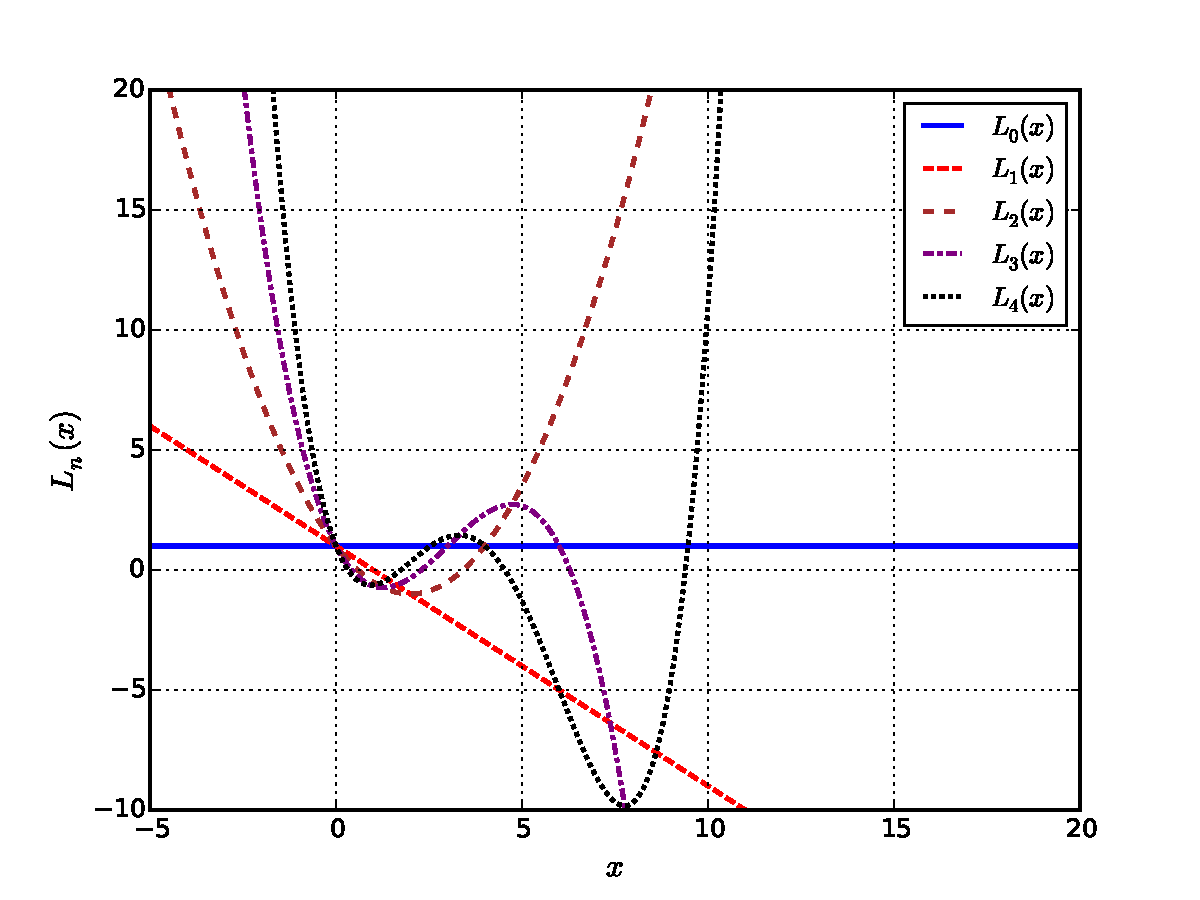
\includegraphics[height=7cm,angle=0]{figs/fig-Laguerre.pdf}}
\caption{Funciones de Laguerre}
\end{figure}

\subsubsection{Ecuaci'on diferencial}

\begin{equation}
x\frac{d^{2}y}{dx^{2}}+(1-x)\frac{dy}{dx}+ny=0
\end{equation}

\subsubsection{Ecuaci'on diferencial (forma de Sturm-Liouville)}

\begin{equation}
\frac{d}{dx}\left[\left(xe^{-x} \right)\frac{dy}{dx}\right]+ne^{-x}y=0
\end{equation}

\subsubsection{F'ormula de Rodrigues}

\begin{equation}
L_{n}(x)=\frac{e^{x}}{n!}\frac{d^{n}}{dx^{n}}(x^{n}e^{-x})
\end{equation}

\subsubsection{Funci'on generadora}

\begin{equation}
\frac{e^{-\frac{xt}{1-t}}}{(1-t)}=\sum_{n=0}^{\infty}\frac{L_{n}(x)}{n!}t^{n}
\end{equation}

\subsubsection{Relaciones de Recurrencia}

\begin{equation}
(n+1)L_{n+1}(x)=(2n+1-x)L_{n}(x)-n^{2}L_{n-1}(x)
\end{equation}

\subsubsection{Ortogonalidad}

\begin{equation}
\int_{0}^{\infty}L_{m}(x)L_{n}(x)e^{-x}\,dx=\delta_{mn}
\end{equation}

\newpage
\section{Funciones de Laguerre asociadas}

\subsubsection{Ecuaci'on diferencial}

\begin{equation}
x\frac{d^{2}y}{dx^{2}}+(k+1-x)\frac{dy}{dx}+ny=0
\end{equation}

\subsubsection{Ecuaci'on diferencial (forma de Sturm-Liouville)}

\begin{equation}
\frac{d}{dx}\left[\left(x^{k+1}e^{-x} \right)\frac{dy}{dx}\right]+ne^{-x}x^{k}y=0
\end{equation}

\subsubsection{F'ormula de Rodrigues}

\begin{equation}
L_{n}^{k}(x)=\frac{e^{x}x^{-k}}{n!}\frac{d^{n}}{dx^{n}}(x^{n+k}e^{-x})
\end{equation}

\subsubsection{Funci'on generadora}

\begin{equation}
(-1)^{k}\, t^{k} \frac{e^{-\frac{xt}{1-t}}}{(1-t)^{k+1}}=\sum_{n=0}^{\infty}\frac{L^{k}_{n}(x)}{n!}t^{n}
\end{equation}

\subsubsection{Relaciones de Recurrencia}

\begin{equation}
\frac{n-k+1}{n+1} L_{n+1}^{k}(x) + \Big(x+m-2n-1\Big) L_n^m(x) + n^2 L^m_{n-1}(x) = 0
\end{equation}


\subsubsection{Ortogonalidad}

\begin{equation}
\int_{0}^{\infty}L^k_{m}(x)L^k_{n}(x)e^{-x}x^{k}\,dx=\frac{\Gamma(n+k+1)!}{n!}\delta_{mn}
\end{equation}

\subsubsection{Aplicaci'on en F'isica}
\begin{itemize}
\item Soluci'on radial de ecuaci'on de Schr\"odinger en potencial de Coulomb ('atomo hidrogenoide).
\end{itemize}


\newpage
\section{Funciones de Hermite}

\subsubsection{Gr'aficos}
\begin{figure}[!h]
\centerline{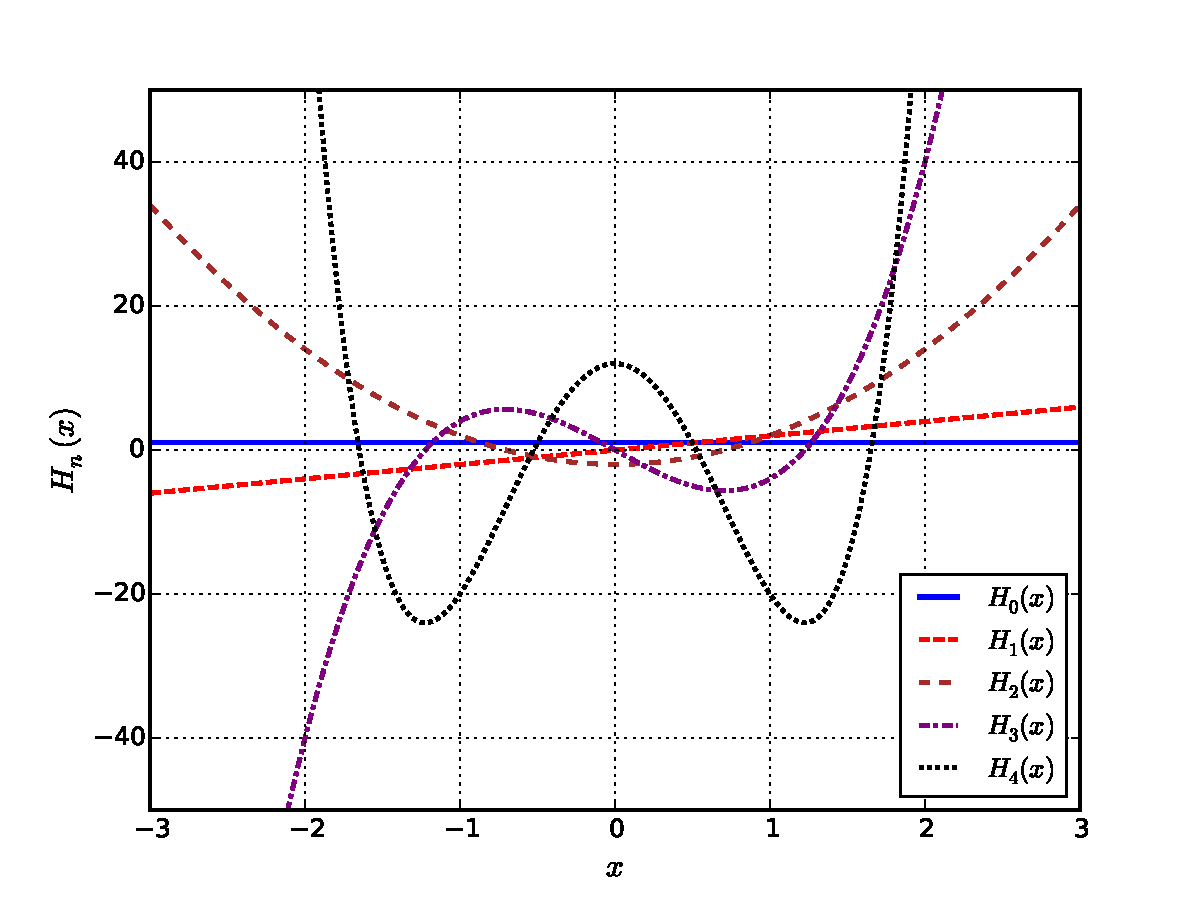
\includegraphics[height=7cm]{figs/fig-Hermite.pdf}}
\caption{Funciones de Hermite}
\end{figure}

\subsubsection{Ecuaci'on diferencial}

\begin{equation}
\frac{d^{2}y}{dx^{2}}-2x\frac{dy}{dx}+2ny=0
\end{equation}

\subsubsection{Ecuaci'on diferencial (forma de Sturm-Liouville)}

\begin{equation}
\frac{d}{dx}\left[\left( e^{-x^{2}}\right)\frac{dy}{dx}\right]+2ne^{-x^{2}}y=0
\end{equation}

\subsubsection{F'ormula de Rodrigues}

\begin{equation}
H_{n}(x)=(-1)^{n}e^{x^{2}}\frac{d^{n}}{dx^{n}}e^{-x^{2}}
\end{equation}

\subsubsection{Funci'on generadora}

\begin{equation}
e^{2tx-t^{2}}=\sum_{n=0}^{\infty}\frac{H_{n}(x)}{n!}t^{n}
\end{equation}

\subsubsection{Relaciones de Recurrencia}

\begin{equation}
H_{n+1}(x)=2xH_{n}(x)-2nH_{n-1}(x)
\end{equation}

\subsubsection{Ortogonalidad}
\begin{equation}
\int_{-\infty}^{\infty}H_{m}(x)H_{n}(x)e^{-x^{2}}\,dx=2^{n}n!\sqrt{\pi}\delta_{mn}
\end{equation}

\subsubsection{Aplicaci'on en F'isica}
\begin{itemize}
\item Oscilador arm'onico cu'antico
\end{itemize}

\newpage
\section{Polinomios de Chebyshev}
\subsubsection{Gr'aficos}
\begin{figure}[!h]
\centerline{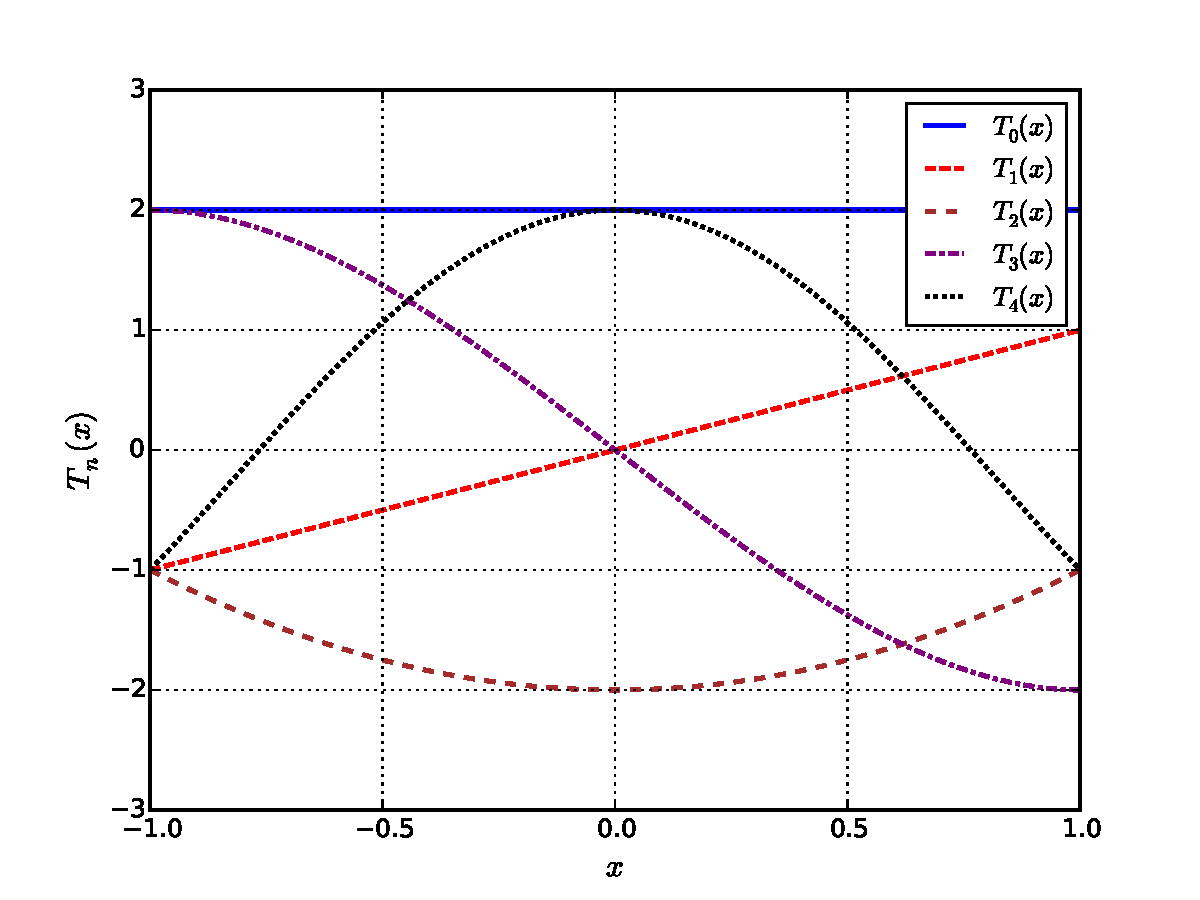
\includegraphics[height=7cm]{figs/fig-Chebyshev.pdf}}
\caption{Polinomios de Chebyshev}
\end{figure}
\url{http://en.wikipedia.org/wiki/File:Chebyshev_Polynomials_of_the_1st_Kind_(n\%3D0-5,_x\%3D(-1,1)).svg}


\subsubsection{Ecuaci'on diferencial}

\begin{equation}
(1-x^{2})\frac{d^{2}y}{dx^{2}}-x\frac{dy}{dx}+n^{2}y=0
\end{equation}

\subsubsection{Ecuaci'on diferencial (forma de Sturm-Liouville)}

\begin{equation}
\frac{d}{dx}\left[\left(\sqrt{1-x^{2}} \right)\frac{dy}{dx}\right]+\frac{n^{2}}{\sqrt{1-x^{2}}}y=0
\end{equation}

\subsubsection{F'ormula de Rodrigues}

\begin{equation}
T_{n}(x)=\frac{(-1)^{n}\sqrt{1-x^{2}}}{(2n-1)(2n-3)\cdots 1} \frac{d^{n}}{dx^{n}}(1-x^{2})^{n-\frac{1}{2}}
\end{equation}

\subsubsection{Funci'on generadora}

\begin{equation}
\frac{1-tx}{1-2tx+t^{2}}=\sum_{n=0}^{\infty}T_{n}(x)t^{n}
\end{equation}

\subsubsection{Relaciones de Recurrencia}

\begin{equation}
T_{n+1}(x)=2xT_{n}(x)-T_{n-1}(x)
\end{equation}

\subsubsection{Ortogonalidad}

\begin{equation}
\int_{-1}^{1}\frac{T_{m}(x)T_{n}(x)}{\sqrt{1-x^{2}}}\,dx= \left\{\begin{array}{ll}\pi & m=n=0\\ \frac{\pi}{2}\delta_{mn} & m=n=N \in \mathbb{N} \end{array}\right.
\end{equation}

\subsubsection{Aplicaci'on en F'isica}
\begin{itemize}
\item Soluci'on num'erica de ecuaciones de fluidos.
\end{itemize}
\chapter{La Delta de Dirac}\label{app:Dirac}
\section{La funci'on $\delta$}
Decimos que $\delta(x)$ es una \textit{delta de Dirac}, si
\begin{equation}
\delta (x-a) = 0\quad \forall x\not = a,
\end{equation}
donde $a\in {\bf R}$, pero
\begin{equation}
\int_b^cf(x)\delta(x-a) d x = \left\{\begin{array}{ccl}
 0 & \text{si} & x\notin (b,c) ,\\
f(a)& \text{si} & x\in (b,c) ,
\end{array}\right.
\end{equation}
para toda funci'on $f$ de clase $C^1$.

 La noci'on general de una delta de Dirac es que 'esta se anula para todo punto,
excepto en $x=a$, y que all'i ``asume un valor divergente'', pero tal que
\begin{equation}
  \int_{-\infty}^{\infty}\delta(x-a)d x = 1.
 \end{equation}
 La delta de Dirac, que en realidad no es una funci'on en sentido estricto,
puede ser entendida como el \textit{l'imite de una sucesi'on de funciones}.
Por ejemplo, si definimos
\begin{equation}
  D_n(x-a) := \sqrt\frac n\pi\cdot e^{-n(x-a)^2}, \qquad n=1,2,3,\dots,
\end{equation}
entonces es posible probar que
\begin{equation}
\int_{-\infty}^{\infty}D_n(x) d x =  1,
\end{equation}
y adem'as
\begin{equation}
\lim_{n\to\infty} D_n(x) =  \left\{\begin{array}{l}0 \quad \forall x\neq
a,\\\infty \quad \text{para }      x=a.\end{array}\right.
\end{equation}
\begin{equation}
\lim_{n\to\infty}\int_b^cD_n(x)f(x)d x = \left\{\begin{array}{ccl}
 0 & \text{si} & x\notin (b,c) ,\\
f(a)& \text{si} & x\in (b,c) .
\end{array}\right.
\end{equation}
Por lo tanto, escribimos
\begin{equation}
  \lim_{n\to\infty}D_n(x)=\delta(x-a).
 \end{equation}
 Una descripci'on matem'aticamente consistente de la delta de Dirac puede ser
dada en el marco de la teor'ia de distribuciones.

Otros ejemplos de sucesiones de funciones que convergen a una Delta de Dirac $\delta(x)$ son:
\begin{equation}
D_n(x)=\frac{n}{\pi}\frac{1}{1+n^2x^2},
\end{equation}
\begin{equation}
D_n(x)=\frac{1}{n\pi}\frac{\sen^2(nx)}{x^2}.
\end{equation}


\subsection{Derivada de la delta de Dirac}

Considerando la funci'on $\delta$ como si fuese una funci'on normal,
encontramos, integrando por partes, que
\begin{equation}
  \int_{-\infty}^{\infty}\underbrace{\delta'(x-a)}_{:=\frac{d}{dx}
   \delta(x-a)} f(x)d x =\underbrace{[\delta(x-a)
   f(x)]_{-\infty}^{\infty}}_{=0}
  -\int_{-\infty}^{\infty}\delta(x-a)f'(x)d x = -f'(a),
 \end{equation}
es decir,
\begin{equation}
  \int_{-\infty}^{\infty}\delta'(x-a) f(x) d x = -f'(a).
 \end{equation}

\section{Delta de Dirac evaluada en una funci'on y cambios de variable}
Por otro lado, de las reglas de cambio de variables, obtenemos
\begin{equation}
\boxed{  \delta(g(x)) = \sum_i\frac{\delta(x-x_i)}{\left|g'(x)\right|},}
 \end{equation}
 donde $x_i$ son las soluciones nulas (simples!) de $g$, e.d., que satisfacen
$g(x)=0$.

Por ejemplo,
\begin{equation}
\boxed{\delta(a x) = \frac{1}{\mid a \mid} \delta(x).}\label{deltaax}
\end{equation}
Esto puede probarse de la forma siguiente: Si $a > 0$ el cambio de variable de
integraci'on $y = a x$ conduce a
\begin{equation}
\int_{- \infty}^{\infty} \delta(a x) f(x)\,d x =
\int_{- \infty}^{\infty} \delta(y) f(\frac{y}{a})\,dy = \frac{1}{a} f(0) =
\int_{- \infty}^{\infty} \frac{1}{a} \delta(x) f(x) \,dx.
\end{equation}
Si $a < 0$, entonces el mismo cambio de variable conduce a
\begin{equation}
\int_{- \infty}^{\infty} \delta(a x) f(x)\,dx =
\int_{\infty}^{- \infty} \delta(y) f(\frac{y}{a})\,dy = - \frac{1}{a} f(0) =
- \int_{- \infty}^{\infty} \frac{1}{a} \delta(x) f(x)\,dx.
\end{equation}
Estos dos resultados son equivalentes a la identidad (\ref{deltaax}).

Como caso particular, si $a=-1$ (\ref{deltaax}), encontramos
\begin{equation}
\boxed{\delta(-x) = \delta(x),}
\end{equation}
e.d., la funci'on $\delta$ es una funci'on par.

\subsection{Otras identidades}
La identidad
\begin{equation}
\boxed{s(x + a) \delta(x) = s(a) \delta(x),}\label{sdelta}
\end{equation}
donde $s(x)$ es una funci'on continua y $a$ una constante, se sigue de
\begin{equation}
\int_{- \infty}^{\infty} s(x + a) \delta(x) f(x)\,dx = s(a) f(0) =
\int_{- \infty}^{\infty} s(a) \delta(x) f(x)\,dx .
\end{equation}
Un caso particular de (\ref{sdelta}) es
\begin{equation}
\boxed{x \delta(x) = 0 .}
\end{equation}

\subsection{Representaci'on integral}\label{sec:DiracFourier}
La expresi'on
\begin{equation}
\boxed{\delta(x) = \frac{1}{2 \pi} \int_{-\infty}^{\infty} e^{i k x}\,d k}
\label{DiracFourier}
\end{equation}
puede ser derivada de la siguiente forma: La transformada de Fourier
$\tilde{f}(k)$ de una funci'on $f(x)$ es definida por
\begin{equation}
f(x) = \frac{1}{2 \pi} \int_{- \infty}^{\infty} e^{i k x } \tilde{f}(k)\,dk ,
\label{Fourier1}
\end{equation}
donde
\begin{equation}
 \tilde{f}(k) := \int_{- \infty}^{\infty} e^{- i k x } f(x)\,dx.
\end{equation}
Para $f(x)=\delta(x)$ obtenemos
\begin{equation}
 \tilde{f}(k) := \int_{- \infty}^{\infty} e^{- i k x } \delta(x)\,dx=\left.e^{-
i k x}\right|_{x=0}=1,
\end{equation}
de modo que (\ref{Fourier1}) se reduce a (\ref{DiracFourier}).

\subsection{La delta de Dirac tridimensional}
 La definici'on de la delta de Dirac tridimensional $\delta^{(3)}(\vec x-\vec
a)$ es an'aloga a aquella de la versi'on unidimensional:
\begin{equation}
  \delta^{(3)}(\vec x-\vec a) = 0,\qquad \forall\  \vec x\not=\vec a ,
\end{equation}
pero
\begin{equation}
  \int_V \delta^{(3)}(\vec x-\vec a) f(\vec x)\,dV = \left\{\begin{array}{ccl}
 0 & \text{si} & \vec{a}\notin V ,\\
f(\vec{a})& \text{si} & \vec{a}\in V .
\end{array}\right.
\end{equation}
 Esta definici'on puede ser usada, por ejemplo, para describir la densidad
de carga de una carga puntual situada en $\vec{x}'$:
\begin{equation}
  \rho(\vec{x}) = q\,\delta^{(3)}(\vec x-\vec{x}'),
 \end{equation}
de modo que
\begin{equation}
 \int_{R^3}\rho(\vec x)\, dV= q.
\end{equation}
 Adem'as, la siguiente identidad es de mucha utilidad:
\begin{equation}
  \boxed{\nabla^2\frac 1{|\vec x-\vec x'|} = -4\pi\,\delta^3(\vec x-\vec x').}
\label{dreid1}
\end{equation}
Para probar esta identidad, debe mostrarse que: a) $\nabla^2\frac 1{|\vec x-\vec
x'|}=0$, $\forall\ \vec x\not= \vec x'$, lo que puede ser directamente
comprobado calculando las derivadas respectivas, y b)  $\int_V
f(\vec x)\nabla^2\frac 1{|\vec x-\vec x'|}\, dV=-4\pi f(\vec x')$  para
cualquier funci'on de clase $C^1$ en el volumen $V$, que contiene el punto $\vec
x'$. Para probar esto 'ultimo, es conveniente usar coordenadas esf'ericas
centradas en el punto $\vec x'$, de modo que $\frac 1{|\vec x-\vec
x'|}=\frac{1}{r}$. Adem'as, como la propiedad a) es v'alida es posible
reemplazar el dominio de integraci'on $V$ (que incluye el punto $\vec x'$) por
una esfera $E$ de radio $R$, centrada en $\vec x'$, de modo que
\begin{eqnarray}
  \int_V f(\vec{x})\nabla^2\frac 1r\, dV &=&
  \int_E f(\vec{x})\nabla^2\frac 1r\, dV \\
&=&\int_E f(\vec
x)\vec\nabla\cdot\left(\vec\nabla\frac {1}{r}\right) \, dV\\
&=&
\int_E\left[\vec\nabla\cdot\left(f\vec\nabla\frac{1}{r}\right)-\vec\nabla
f\cdot \vec\nabla\frac{1}{r}\right]\,
dV\\
&=& \oint_{\partial E}\left(f\vec\nabla\frac{1}{r}\right)\cdot
d\vec{S}
-\int_E \vec\nabla f\cdot \vec\nabla\frac{1}{r}\, dV\\
&=& -\oint_{\partial E}f\frac{1}{r^2}\, (\hat{r}\cdot d\vec{S})
+\int_E (\vec\nabla f\cdot\hat{r})\frac{1}{r^2}\, dV\\
&=& -\oint_{\partial E}f\frac{1}{r^2}\, dS
+\int_E \frac{\partial f}{\partial r}\frac{1}{r^2}\, dV \\
&=& -\oint_{\partial E}f\, d\Omega
+\int_E \frac{\partial f}{\partial r}\, drd\Omega .
\end{eqnarray}
Si $f$ es una funci'on de clase $C^1$, ambos t'erminos son finitos y su suma es
independiente de $R$. En el l'imite $R\rightarrow 0$, el primer t'ermino tiende
a $-f|_{r=0}\oint d\Omega=-4\pi f(\vec x')$, mientras que el segundo tiende a
cero debido a la integral sobre la variable $r$, desde $r=0$ hasta $r=R$. De
este modo, obtenemos
\begin{eqnarray}
  \int_V f(\vec{x})\nabla^2\frac 1r\, dV &=& \lim_{R\rightarrow
0}\left[-\oint_{\partial E}f\, d\Omega+\int_E \frac{\partial f}{\partial r}\,
drd\Omega \right]\\
&=& -4\pi f(\vec x')+0.
\end{eqnarray}

\chapter{Coordenadas curvilineas}

\section{Coordenadas Cartesianas}
\noindent Vector
\begin{eqnarray}
\vec{A}
&=& A_x{\hat x} + A_y {\hat y} + A_z {\hat z}
\end{eqnarray}
Gradiente:
\begin{eqnarray}
 \vec\nabla\Psi&=&{\partial\Psi\over \partial x} {\hat x} + {\partial\Psi\over
\partial y} {\hat y}   + {\partial\Psi\over \partial z} {\hat z}
\end{eqnarray}
Divergencia
\begin{eqnarray}
 \vec\nabla \cdot \vec{A}
&=& \frac{\partial  A_x}{\partial x}+\frac{\partial  A_y}{\partial y}+\frac{\partial  A_z}{\partial z}
\end{eqnarray}
Rotor:
\begin{eqnarray}
\vec\nabla \times  \vec{A}
&=&   \left({\partial A_z \over \partial y} - {\partial A_y \over
\partial z}\right)  {\hat x}  +
   \left({\partial A_x \over \partial z} - {\partial A_z \over
\partial x}\right)  {\hat y}  +
   \left({\partial A_y \over \partial x} - {\partial A_x \over
\partial y}\right)  {\hat z}
\end{eqnarray}
Laplaciano
\begin{eqnarray}
 \nabla^2 \Psi
&=& {\partial^2\Psi\over \partial x^2} + {\partial^2\Psi\over \partial y^2} +
{\partial^2\Psi\over \partial z^2}
\end{eqnarray}
Desplazamiento:
\begin{eqnarray}
 d \vec{x} &=& dx {\hat x} + dy {\hat y} + dz {\hat z}
\end{eqnarray}
Elemento de superficie:
\begin{eqnarray}
 d \vec{S} &=& dy\,dz\, {\hat x} + dx\,dz\, {\hat y} +
dx\,dy\, {\hat z}
\end{eqnarray}
Elemento de volumen:
\begin{eqnarray}
 dV &=& dx\,dy\,dz
\end{eqnarray}

\section{Coordenadas Cil'indricas}
Definici'on:
\begin{equation}
    x  =  \rho\cos\varphi , \qquad
    y  =  \rho\sen\varphi , \qquad
    z =  z
\end{equation}
\begin{equation}
    \rho  =  \sqrt{x^2 + y^2} , \qquad
    \varphi  = \arctan{(y/x)}, \qquad
     z=  z
\end{equation}
Vector
\begin{equation}
\vec{A} =A_\rho {\hat \rho} + A_\varphi {\hat \varphi} +
A_z {\hat z}
\end{equation}
Gradiente:
\begin{eqnarray}
 \vec\nabla\Psi&=&{\partial\Psi\over \partial \rho} {\hat \rho}
  + {1 \over \rho}{\partial\Psi\over \partial \varphi} {\hat \varphi}
  + {\partial\Psi\over \partial z} {\hat z}
\end{eqnarray}
Divergencia
\begin{eqnarray}
 \vec\nabla \cdot \vec{A}
&=&  {1 \over \rho}{\partial \left( \rho A_\rho  \right) \over \partial
\rho}  + {1 \over \rho}{\partial A_\varphi \over \partial \varphi}
  + {\partial A_z \over \partial z}
\end{eqnarray}
Rotor:
\begin{eqnarray}
\vec\nabla \times  \vec{A}
&=&   \left({1 \over \rho}{\partial A_z \over \partial \varphi}
    - {\partial A_\varphi \over \partial z}\right)  {\hat \rho} +
\left({\partial A_\rho \over \partial z} - {\partial A_z \over
\partial \rho}\right)  {\hat \varphi} \nonumber\\
&&+  {1 \over \rho}\left({\partial \left( \rho A_\varphi \right) \over
\partial \rho}     - {\partial A_\rho \over \partial \varphi}\right) {\hat z}
\end{eqnarray}
Laplaciano
\begin{eqnarray}
 \nabla^2 \Psi
&=& {1 \over \rho}{\partial \over \partial \rho}\left(\rho {\partial\Psi\over
\partial \rho}\right)
  + {1 \over \rho^2}{\partial^2\Psi\over \partial \varphi^2}
  + {\partial^2\Psi\over \partial z^2} \\
\end{eqnarray}
Desplazamiento:
\begin{eqnarray}
 d \vec{x}
 &=& d\rho {\hat \rho} + \rho d\varphi {\hat \varphi} +dz {\hat z}
\end{eqnarray}
Elemento de superficie:
\begin{eqnarray}
 d \vec{S}
&=& \rho\, d\varphi\, dz\, {\hat \rho} + d\rho
\,dz\, {\hat \varphi} +  \rho \,d\rho\, d\varphi \, {\hat z}
\end{eqnarray}
Elemento de volumen:
\begin{eqnarray}
 dV
 &=& \rho\, d\rho\, d\varphi\, dz
\end{eqnarray}

\section{Coordenadas Esf'ericas}
Definici'on:
\begin{equation}
    x  =  r\sen\theta\cos\varphi, \qquad
    y  =  r\sen\theta\sen\varphi , \qquad
    z  =  r\cos\theta
\end{equation}
\begin{equation}
    r  =  \sqrt{x^2 + y^2 + z^2} , \quad
    \theta  =  \arccos(\frac{z}{r}) = \arctan{\frac{\sqrt{x^2+y^2}}{z}}, \quad
    \varphi  =  \arctan{(y/x)}
\end{equation}
Vector
\begin{eqnarray}
\vec{A}
&=& A_r {\hat r} + A_\theta {\hat \theta} +
A_\varphi {\hat \varphi}
\end{eqnarray}
Gradiente:
\begin{eqnarray}
 \vec\nabla\Psi
 &=& {\partial\Psi\over \partial r} {\hat r}
  + {1 \over r}{\partial\Psi\over \partial \theta} {\hat \theta}
  + {1 \over r\sen\theta}{\partial\Psi\over \partial \varphi} {\hat \varphi}
\end{eqnarray}
Divergencia
\begin{eqnarray}
 \vec\nabla \cdot \vec{A}
&=& {1 \over r^2}{\partial \left( r^2 A_r \right) \over \partial r}
  + {1 \over r\sen\theta}{\partial \over \partial \theta} \left(
A_\theta\sen\theta \right)
  + {1 \over r\sen\theta}{\partial A_\varphi \over \partial \varphi}
\end{eqnarray}
Rotor:
\begin{eqnarray}
\vec\nabla \times  \vec{A}
&=&  {1 \over r\sen\theta}\left({\partial \over \partial \theta}
\left( A_\varphi\sen\theta \right)    - {\partial A_\theta \over \partial
\varphi}\right) {\hat r} \nonumber\\
&&+    {1 \over r}\left({1 \over \sen\theta}{\partial A_r \over \partial
\varphi} - {\partial \over \partial r} \left( r A_\varphi \right) \right)
 {\hat \theta}  +   {1 \over r}\left({\partial \over \partial r} \left( r
A_\theta
\right)  - {\partial A_r \over \partial \theta}\right)  {\hat \varphi}
\end{eqnarray}
Laplaciano
\begin{eqnarray}
 \nabla^2 \Psi
&=&  {1 \over r^2}{\partial \over \partial r}\left(r^2 {\partial\Psi\over
\partial r}\right)   + {1 \over r^2\sen\theta}{\partial \over \partial
\theta}\left(\sen\theta {\partial\Psi\over \partial \theta}\right)
  + {1 \over r^2\sen^2\theta}{\partial^2\Psi\over \partial \varphi^2}
\end{eqnarray}
Desplazamiento:
\begin{eqnarray}
 d \vec{x}
&= & dr {\hat r} + rd\theta {\hat \theta} +r\sen\theta d\varphi {\hat \varphi}
\end{eqnarray}
Elemento de superficie:
\begin{eqnarray}
 d \vec{S}
&=& r^2 \sen\theta \,d\theta \,d\varphi \, {\hat r} + r\sen\theta
\,dr\,d\varphi \, {\hat \theta} +  r\,dr\,d\theta\, {\hat \varphi}
\end{eqnarray}
Elemento de volumen:
\begin{eqnarray}
 dV
&=& r^2\sen\theta \,dr\,d\theta\, d\varphi
\end{eqnarray}
Soluci'on general (finita) de la Ecuaci'on de Laplace:
\begin{equation}
\Psi(r,\theta,\varphi) = \sum_{l=0}^\infty\sum_{m=-l}^l\left[
A_{lm}\cdot r^l + B_{lm}\cdot r^{-(l+1)}\right]\cdot Y_{lm}(\theta,\varphi).
\label{est31}
\end{equation}


\begin{thebibliography}{99}
\bibitem{Mauch} Sean Mauch, {\em Introduction to Methods of Applied Mathematics                           or Advanced Mathematical Methods for Scientists and Engineers} (2011), 
\url{http://www.its.caltech.edu/~sean/}. \url{https://bitbucket.org/seanmauch/applied_math}.
\bibitem{Arfken} G. Arfken and H.Weber, {\em Mathematical Methods for Physicists}, Fifth Edition, Academic Press, (2001).
\bibitem{Butkov} E. Butkov, {\em Mathematical Physics}, Addison-Wesley (1968).
\bibitem{Hassani} S. Hassani. {\em Mathematical Physics: A Modern Introduction to Its Foundations}, Springer (1999).
\item L. Santal'o, {\em Vectores y Tensores con sus aplicaciones}, Editorial Universitaria de Buenos Aires, S'eptima Edici'on (1969).
\end{thebibliography}


\end{document}
